
\begin{figure}
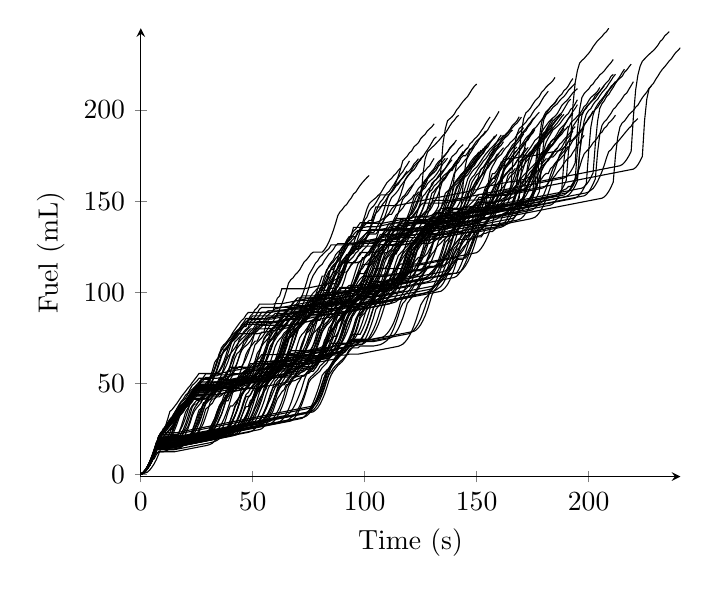
\begin{tikzpicture}
\begin{axis}[
legend style={anchor=west},
axis x line=bottom,
axis y line=left,
ymin=-1,
xlabel=Time (s),
ylabel=Fuel (mL),
]
\addplot[] coordinates {
(0, 0.239885513361)
(1, 1.00158279561)
(2, 2.23953091171)
(3, 3.903534361)
(4, 6.00694100463)
(5, 8.49987930335)
(6, 11.3619771435)
(7, 14.7682910646)
(8, 18.7422527596)
(9, 22.5020939837)
(10, 23.7631839559)
(11, 25.6355657875)
(12, 26.6865086892)
(13, 28.4867889769)
(14, 29.5226751874)
(15, 31.2452994042)
(16, 33.2560150228)
(17, 34.4260663708)
(18, 36.4957196646)
(19, 38.157493437)
(20, 39.5418113984)
(21, 41.5401129326)
(22, 43.0902482159)
(23, 44.7972590926)
(24, 45.9083429747)
(25, 47.7068966186)
(26, 48.8415414835)
(27, 48.8415414835)
(28, 48.8415414835)
(29, 48.8415414835)
(30, 50.551673038)
(31, 52.6081826576)
(32, 55.19645185)
(33, 58.2960753756)
(34, 61.7999585748)
(35, 65.7517822136)
(36, 69.596987394)
(37, 71.2117604695)
(38, 72.3662352324)
(39, 73.8931285837)
(40, 75.555259631)
(41, 77.7666876071)
(42, 79.5543660498)
(43, 81.3156155485)
(44, 82.9853217468)
(45, 84.5937854948)
(46, 85.6222530087)
(47, 87.5689801598)
(48, 88.989140597)
(49, 88.989140597)
(50, 88.989140597)
(51, 88.989140597)
(52, 88.989140597)
(53, 88.989140597)
(54, 88.989140597)
(55, 88.989140597)
(56, 88.989140597)
(57, 88.989140597)
(58, 88.989140597)
(59, 89.2290261103)
(60, 89.4689116237)
(61, 89.7087971371)
(62, 89.9486826504)
(63, 90.1885681638)
(64, 90.4284536772)
(65, 90.6683391905)
(66, 90.9082247039)
(67, 91.1481102172)
(68, 91.3879957306)
(69, 91.627881244)
(70, 91.8677667573)
(71, 92.1076522707)
(72, 92.347537784)
(73, 92.5874232974)
(74, 92.8273088108)
(75, 93.0671943241)
(76, 93.4382717921)
(77, 94.0117854362)
(78, 94.8553739392)
(79, 96.3267010969)
(80, 98.4256667478)
(81, 101.065692166)
(82, 103.216417424)
(83, 106.707412927)
(84, 110.804487183)
(85, 112.56912833)
(86, 112.56912833)
(87, 115.12305612)
(88, 117.435182754)
(89, 119.381113042)
(90, 123.444155171)
(91, 124.896877069)
(92, 127.03960039)
(93, 128.228587696)
(94, 129.546456599)
(95, 131.699021069)
(96, 133.056085465)
(97, 134.024728209)
(98, 134.024728209)
(99, 134.024728209)
(100, 134.024728209)
(101, 134.024728209)
(102, 134.024728209)
(103, 134.024728209)
(104, 134.024728209)
(105, 134.024728209)
(106, 134.264613723)
(107, 134.504499236)
(108, 134.744384749)
(109, 134.984270263)
(110, 135.224155776)
(111, 135.464041289)
(112, 135.703926803)
(113, 135.943812316)
(114, 136.183697829)
(115, 136.423583343)
(116, 136.663468856)
(117, 136.90335437)
(118, 137.143239883)
(119, 137.383125396)
(120, 137.62301091)
(121, 137.862896423)
(122, 138.102781936)
(123, 138.34266745)
(124, 138.582552963)
(125, 138.822438476)
(126, 139.06232399)
(127, 139.302209503)
(128, 139.542095016)
(129, 140.317756321)
(130, 141.48240256)
(131, 143.052877124)
(132, 145.006809188)
(133, 147.40723723)
(134, 166.933639763)
(135, 181.918374676)
(136, 189.659096515)
(137, 194.172292315)
(138, 195.261055371)
(139, 196.322158477)
(140, 197.780045557)
(141, 200.000986586)
(142, 201.471407853)
(143, 203.25357643)
(144, 204.885153303)
(145, 206.220340495)
(146, 207.522294096)
(147, 209.487013249)
(148, 211.463601131)
(149, 213.090100577)
(150, 214.230191817)
};
\addplot[] coordinates {
(0, 0.239885513361)
(1, 0.88832512986)
(2, 1.92149619989)
(3, 3.35706014906)
(4, 5.13319416558)
(5, 7.27564914071)
(6, 9.93924772103)
(7, 13.0406715656)
(8, 16.7629814886)
(9, 16.7629814886)
(10, 16.7629814886)
(11, 16.7629814886)
(12, 16.7629814886)
(13, 16.7629814886)
(14, 16.7629814886)
(15, 17.002867002)
(16, 17.2427525153)
(17, 17.4826380287)
(18, 17.7225235421)
(19, 17.9624090554)
(20, 18.2022945688)
(21, 18.4421800821)
(22, 18.6820655955)
(23, 18.9219511089)
(24, 19.1618366222)
(25, 19.4017221356)
(26, 19.6416076489)
(27, 19.8814931623)
(28, 20.1213786757)
(29, 20.361264189)
(30, 20.6011497024)
(31, 20.8410352158)
(32, 21.0809207291)
(33, 21.3208062425)
(34, 21.5606917558)
(35, 21.8005772692)
(36, 22.0404627826)
(37, 22.2803482959)
(38, 22.5202338093)
(39, 22.7601193226)
(40, 23.0321547206)
(41, 23.6210035067)
(42, 24.1924199077)
(43, 25.3964193971)
(44, 26.8882579951)
(45, 28.7713132548)
(46, 30.3354115562)
(47, 31.6319795075)
(48, 34.8969316013)
(49, 37.9722581202)
(50, 42.1643906364)
(51, 44.122308214)
(52, 46.8127744346)
(53, 47.7996931681)
(54, 49.1913568863)
(55, 51.1224631597)
(56, 51.1224631597)
(57, 53.7722522288)
(58, 55.6728036825)
(59, 56.8511689341)
(60, 56.8511689341)
(61, 56.8511689341)
(62, 56.8511689341)
(63, 56.8511689341)
(64, 56.8511689341)
(65, 56.8511689341)
(66, 56.8511689341)
(67, 56.8511689341)
(68, 56.8511689341)
(69, 57.2217419725)
(70, 58.0810985)
(71, 58.9290173206)
(72, 59.5172641106)
(73, 60.4049497384)
(74, 60.9662521105)
(75, 62.6609164)
(76, 62.6609164)
(77, 64.800376271)
(78, 67.4195874868)
(79, 70.5151319336)
(80, 73.9713090164)
(81, 78.0610736063)
(82, 80.9884284297)
(83, 82.6563511104)
(84, 84.6637660111)
(85, 86.7419308034)
(86, 87.9268139123)
(87, 89.2914955139)
(88, 91.2437969508)
(89, 92.3386885196)
(90, 92.3386885196)
(91, 92.3386885196)
(92, 92.3386885196)
(93, 92.3386885196)
(94, 92.3386885196)
(95, 93.3492255515)
(96, 93.3492255515)
(97, 93.3492255515)
(98, 93.924183123)
(99, 94.5340040676)
(100, 94.5340040676)
(101, 94.9208497943)
(102, 94.9208497943)
(103, 94.9208497943)
(104, 94.9208497943)
(105, 94.9208497943)
(106, 94.9208497943)
(107, 94.9208497943)
(108, 95.1607353077)
(109, 95.4006208211)
(110, 95.6405063344)
(111, 95.8803918478)
(112, 96.1202773612)
(113, 96.3601628745)
(114, 96.6000483879)
(115, 96.8399339012)
(116, 97.0798194146)
(117, 97.319704928)
(118, 97.5595904413)
(119, 97.7994759547)
(120, 98.039361468)
(121, 98.2792469814)
(122, 98.5191324948)
(123, 98.7590180081)
(124, 98.9989035215)
(125, 99.2387890349)
(126, 99.4786745482)
(127, 99.7185600616)
(128, 99.9584455749)
(129, 100.198331088)
(130, 100.438216602)
(131, 100.804139179)
(132, 101.453412511)
(133, 102.31121179)
(134, 103.261958095)
(135, 104.858679082)
(136, 107.08174994)
(137, 109.840023962)
(138, 113.165222358)
(139, 116.832782493)
(140, 121.081948066)
(141, 123.256269826)
(142, 124.316697361)
(143, 125.492372514)
(144, 127.568628997)
(145, 129.092796115)
(146, 130.408308277)
(147, 132.462533102)
(148, 134.592336265)
(149, 136.635220343)
(150, 138.457837802)
(151, 139.613408083)
(152, 140.879925781)
(153, 140.879925781)
(154, 140.879925781)
(155, 140.879925781)
(156, 140.879925781)
(157, 140.879925781)
(158, 140.879925781)
(159, 140.879925781)
(160, 140.879925781)
(161, 140.879925781)
(162, 141.119811294)
(163, 141.359696807)
(164, 141.599582321)
(165, 141.839467834)
(166, 142.079353347)
(167, 142.319238861)
(168, 142.559124374)
(169, 142.799009887)
(170, 143.038895401)
(171, 143.278780914)
(172, 143.518666428)
(173, 143.758551941)
(174, 143.998437454)
(175, 144.238322968)
(176, 144.478208481)
(177, 144.718093994)
(178, 144.957979508)
(179, 145.197865021)
(180, 145.437750534)
(181, 145.677636048)
(182, 145.917521561)
(183, 146.157407075)
(184, 146.397292588)
(185, 146.637178101)
(186, 146.877063615)
(187, 147.116949128)
(188, 147.356834641)
(189, 147.596720155)
(190, 147.836605668)
(191, 148.076491181)
(192, 148.316376695)
(193, 148.556262208)
(194, 148.796147721)
(195, 149.036033235)
(196, 149.275918748)
(197, 149.515804262)
(198, 149.755689775)
(199, 149.995575288)
(200, 150.235460802)
(201, 150.475346315)
(202, 150.715231828)
(203, 150.955117342)
(204, 151.195002855)
(205, 151.434888368)
(206, 151.674773882)
(207, 152.396595089)
(208, 153.674685343)
(209, 155.41046824)
(210, 157.711425045)
(211, 160.471739046)
(212, 175.136338567)
(213, 185.125354365)
(214, 190.708135207)
(215, 192.971270765)
(216, 193.977842055)
(217, 195.681449402)
(218, 197.466508602)
(219, 198.732699495)
(220, 199.722632399)
(221, 201.54518373)
(222, 202.698516268)
(223, 204.779679453)
(224, 206.797388974)
(225, 208.377202828)
(226, 209.861879877)
(227, 211.930543761)
(228, 213.206809826)
};
\addplot[] coordinates {
(0, 0.239885513361)
(1, 1.0262980486)
(2, 2.23162916632)
(3, 3.75951917318)
(4, 5.73297699408)
(5, 8.23602456628)
(6, 11.2357794658)
(7, 14.8019694307)
(8, 18.761057791)
(9, 18.761057791)
(10, 18.761057791)
(11, 18.761057791)
(12, 18.761057791)
(13, 18.761057791)
(14, 18.761057791)
(15, 18.761057791)
(16, 18.761057791)
(17, 18.761057791)
(18, 18.761057791)
(19, 19.0009433044)
(20, 19.2408288177)
(21, 19.4807143311)
(22, 19.7205998445)
(23, 19.9604853578)
(24, 20.2003708712)
(25, 20.4402563846)
(26, 20.6801418979)
(27, 20.9200274113)
(28, 21.1599129246)
(29, 21.399798438)
(30, 21.7968880722)
(31, 22.8498634233)
(32, 24.4116528959)
(33, 25.7914443514)
(34, 27.7133613137)
(35, 30.6131064261)
(36, 33.0315215682)
(37, 36.624466546)
(38, 40.583258291)
(39, 44.4050426053)
(40, 45.4854529388)
(41, 47.345239933)
(42, 49.0657108493)
(43, 50.4336492971)
(44, 52.5787521701)
(45, 54.0647361734)
(46, 55.2782076001)
(47, 57.1630046979)
(48, 58.7635762738)
(49, 60.9237022386)
(50, 60.9237022386)
(51, 60.9237022386)
(52, 60.9237022386)
(53, 60.9237022386)
(54, 60.9237022386)
(55, 60.9237022386)
(56, 60.9237022386)
(57, 60.9237022386)
(58, 60.9237022386)
(59, 61.163587752)
(60, 61.4034732654)
(61, 61.6433587787)
(62, 61.8832442921)
(63, 62.1231298054)
(64, 62.3630153188)
(65, 62.6029008322)
(66, 62.8427863455)
(67, 63.0826718589)
(68, 63.3225573723)
(69, 63.5624428856)
(70, 63.802328399)
(71, 64.0422139123)
(72, 64.2820994257)
(73, 64.5219849391)
(74, 65.0760978208)
(75, 65.7482656284)
(76, 66.7986671981)
(77, 68.4441662647)
(78, 70.6355182279)
(79, 73.3768619751)
(80, 76.6787754995)
(81, 80.3254187319)
(82, 84.4643490576)
(83, 86.7614755712)
(84, 89.1435383775)
(85, 90.6282947832)
(86, 90.6282947832)
(87, 91.9894772928)
(88, 93.0040699521)
(89, 94.8534389728)
(90, 94.8534389728)
(91, 97.7524653462)
(92, 99.4459968996)
(93, 100.652199043)
(94, 100.652199043)
(95, 100.652199043)
(96, 100.652199043)
(97, 100.652199043)
(98, 101.347431355)
(99, 101.347431355)
(100, 103.201291873)
(101, 105.378923415)
(102, 108.028190735)
(103, 111.243769554)
(104, 114.831931463)
(105, 119.026669216)
(106, 121.419834402)
(107, 122.845631472)
(108, 124.061375784)
(109, 126.247472745)
(110, 127.881180574)
(111, 128.938303618)
(112, 131.1247206)
(113, 133.174841672)
(114, 135.106243977)
(115, 136.439182919)
(116, 137.567026616)
(117, 139.392981892)
(118, 139.392981892)
(119, 139.392981892)
(120, 139.392981892)
(121, 139.392981892)
(122, 139.392981892)
(123, 139.392981892)
(124, 139.392981892)
(125, 139.392981892)
(126, 139.392981892)
(127, 139.392981892)
(128, 139.632867406)
(129, 139.872752919)
(130, 140.112638433)
(131, 140.352523946)
(132, 140.592409459)
(133, 140.832294973)
(134, 141.072180486)
(135, 141.312065999)
(136, 141.551951513)
(137, 141.791837026)
(138, 142.031722539)
(139, 142.271608053)
(140, 142.511493566)
(141, 142.75137908)
(142, 142.991264593)
(143, 143.231150106)
(144, 143.47103562)
(145, 143.710921133)
(146, 143.950806646)
(147, 144.19069216)
(148, 144.430577673)
(149, 144.670463186)
(150, 144.9103487)
(151, 145.150234213)
(152, 145.390119727)
(153, 145.63000524)
(154, 145.869890753)
(155, 146.109776267)
(156, 146.34966178)
(157, 146.589547293)
(158, 146.829432807)
(159, 147.06931832)
(160, 147.309203833)
(161, 147.549089347)
(162, 147.78897486)
(163, 148.028860373)
(164, 148.268745887)
(165, 148.5086314)
(166, 148.748516914)
(167, 148.988402427)
(168, 149.22828794)
(169, 149.468173454)
(170, 149.708058967)
(171, 149.94794448)
(172, 150.187829994)
(173, 150.761676482)
(174, 151.782431476)
(175, 153.229308997)
(176, 155.117511273)
(177, 157.608257043)
(178, 177.075043787)
(179, 188.048511796)
(180, 194.771504046)
(181, 197.365719374)
(182, 198.568918468)
(183, 199.670798906)
(184, 201.394808987)
(185, 202.411446944)
(186, 203.433254234)
(187, 205.091545455)
(188, 206.433223416)
(189, 207.478226324)
(190, 209.006105643)
(191, 210.87316518)
(192, 212.081037805)
(193, 213.344785162)
(194, 214.521380464)
};
\addplot[] coordinates {
(0, 0.239885513361)
(1, 0.998781971194)
(2, 2.36229631389)
(3, 4.29140355273)
(4, 6.84820421339)
(5, 9.90979148007)
(6, 13.5108904338)
(7, 17.5205738613)
(8, 21.0080638135)
(9, 22.4015405464)
(10, 24.1282101194)
(11, 25.1964919575)
(12, 26.9129250181)
(13, 27.9249086658)
(14, 29.5387092461)
(15, 30.9783971316)
(16, 32.2624031432)
(17, 33.4049630906)
(18, 35.1881237521)
(19, 36.8653377454)
(20, 38.3656486527)
(21, 39.4003292499)
(22, 40.5030407492)
(23, 41.9544279875)
(24, 43.6448988521)
(25, 43.6448988521)
(26, 43.6448988521)
(27, 43.6448988521)
(28, 43.6448988521)
(29, 43.6448988521)
(30, 43.6448988521)
(31, 43.6448988521)
(32, 43.6448988521)
(33, 43.6448988521)
(34, 43.8847843655)
(35, 44.1246698788)
(36, 44.3645553922)
(37, 44.6044409056)
(38, 44.8443264189)
(39, 45.0842119323)
(40, 45.3240974456)
(41, 45.563982959)
(42, 45.8038684724)
(43, 46.0437539857)
(44, 46.2836394991)
(45, 46.5235250124)
(46, 46.7634105258)
(47, 47.0032960392)
(48, 47.2431815525)
(49, 47.7294161004)
(50, 48.4128364023)
(51, 49.8318913301)
(52, 51.6596106656)
(53, 53.9368395712)
(54, 56.5540405229)
(55, 59.7819671159)
(56, 63.3429458461)
(57, 67.3418449777)
(58, 70.8530583201)
(59, 72.4797161584)
(60, 74.043042446)
(61, 76.1031986425)
(62, 77.5752262882)
(63, 79.1734517308)
(64, 80.3058240655)
(65, 81.857366174)
(66, 84.0686757307)
(67, 85.3701069785)
(68, 86.8541766172)
(69, 88.2202662321)
(70, 88.2202662321)
(71, 88.2202662321)
(72, 89.1630405911)
(73, 89.1630405911)
(74, 89.1630405911)
(75, 90.6710951904)
(76, 92.7608770393)
(77, 95.2518655719)
(78, 98.3001883253)
(79, 101.996424616)
(80, 105.175881658)
(81, 108.908287084)
(82, 108.908287084)
(83, 111.552740639)
(84, 114.517267234)
(85, 116.394564248)
(86, 117.858122015)
(87, 120.531808209)
(88, 122.065958742)
(89, 123.065425018)
(90, 124.963592668)
(91, 126.129575061)
(92, 128.753563901)
(93, 130.500287819)
(94, 130.500287819)
(95, 130.500287819)
(96, 130.500287819)
(97, 132.620251864)
(98, 135.201908358)
(99, 138.124419538)
(100, 141.660149116)
(101, 145.785357419)
(102, 148.593262167)
(103, 149.851325447)
(104, 150.91091053)
(105, 151.91658397)
(106, 153.220456654)
(107, 154.244942081)
(108, 156.252308229)
(109, 158.350131863)
(110, 160.298853415)
(111, 161.523718816)
(112, 162.532367812)
(113, 164.161530148)
(114, 165.254831177)
(115, 166.898730267)
(116, 168.266249567)
};
\addplot[] coordinates {
(0, 0.239885513361)
(1, 0.79435496533)
(2, 1.76292391026)
(3, 3.21471805152)
(4, 5.14538615515)
(5, 7.47214035477)
(6, 10.2746607413)
(7, 13.4768410861)
(8, 17.080039056)
(9, 18.8294278803)
(10, 18.8294278803)
(11, 18.8294278803)
(12, 18.8294278803)
(13, 18.8294278803)
(14, 18.8294278803)
(15, 18.8294278803)
(16, 18.8294278803)
(17, 18.8294278803)
(18, 18.8294278803)
(19, 19.0693133937)
(20, 19.3091989071)
(21, 19.5490844204)
(22, 19.7889699338)
(23, 20.0288554471)
(24, 20.2687409605)
(25, 20.5086264739)
(26, 20.7485119872)
(27, 20.9883975006)
(28, 21.2282830139)
(29, 21.4681685273)
(30, 21.7080540407)
(31, 21.947939554)
(32, 22.1878250674)
(33, 22.4277105808)
(34, 22.6675960941)
(35, 22.9074816075)
(36, 23.1473671208)
(37, 23.3872526342)
(38, 23.6271381476)
(39, 23.8670236609)
(40, 24.1069091743)
(41, 24.3467946876)
(42, 24.586680201)
(43, 24.8265657144)
(44, 25.0664512277)
(45, 25.3063367411)
(46, 25.5462222545)
(47, 25.7861077678)
(48, 26.0259932812)
(49, 26.2658787945)
(50, 26.5057643079)
(51, 26.7456498213)
(52, 26.9855353346)
(53, 27.225420848)
(54, 27.4653063613)
(55, 28.2679770804)
(56, 29.6271900382)
(57, 31.5939336932)
(58, 34.0258113247)
(59, 37.0342846615)
(60, 40.5437046881)
(61, 44.6606932196)
(62, 47.4643429971)
(63, 49.0209331893)
(64, 50.0254435916)
(65, 51.7286013244)
(66, 53.1798530453)
(67, 55.0315216729)
(68, 56.7503659894)
(69, 58.8393892268)
(70, 60.8604992795)
(71, 62.0816425442)
(72, 63.5754683332)
(73, 63.5754683332)
(74, 63.5754683332)
(75, 63.5754683332)
(76, 63.5754683332)
(77, 64.4009715986)
(78, 65.3108589686)
(79, 65.3108589686)
(80, 66.6782026373)
(81, 68.3917406248)
(82, 70.7394806288)
(83, 73.4123217873)
(84, 76.5625349734)
(85, 80.1098803666)
(86, 84.0321114731)
(87, 88.2330400084)
(88, 89.2803970875)
(89, 90.8501284985)
(90, 92.6573596009)
(91, 93.6596360018)
(92, 94.9139150913)
(93, 96.1760897693)
(94, 96.1760897693)
(95, 99.1228852028)
(96, 100.132783465)
(97, 101.690134906)
(98, 102.724093924)
(99, 102.724093924)
(100, 102.724093924)
(101, 102.724093924)
(102, 103.359151855)
(103, 103.359151855)
(104, 103.359151855)
(105, 103.359151855)
(106, 103.359151855)
(107, 103.359151855)
(108, 103.359151855)
(109, 103.359151855)
(110, 103.599037368)
(111, 103.838922882)
(112, 104.078808395)
(113, 104.318693908)
(114, 104.558579422)
(115, 104.798464935)
(116, 105.038350448)
(117, 105.278235962)
(118, 105.518121475)
(119, 105.758006988)
(120, 105.997892502)
(121, 106.237778015)
(122, 106.477663529)
(123, 106.717549042)
(124, 106.957434555)
(125, 107.197320069)
(126, 107.437205582)
(127, 107.677091095)
(128, 107.916976609)
(129, 108.156862122)
(130, 108.396747635)
(131, 108.636633149)
(132, 108.876518662)
(133, 109.116404176)
(134, 109.356289689)
(135, 109.596175202)
(136, 109.836060716)
(137, 110.622820854)
(138, 111.920263661)
(139, 113.645342828)
(140, 115.989120603)
(141, 118.690588549)
(142, 122.008796125)
(143, 125.952159479)
(144, 129.759958227)
(145, 131.794279477)
(146, 133.405904169)
(147, 135.050511975)
(148, 136.032891222)
(149, 138.210722551)
(150, 140.077798965)
(151, 141.873432266)
(152, 143.214058826)
(153, 144.987207676)
(154, 146.813422482)
(155, 148.822725095)
(156, 148.822725095)
(157, 148.822725095)
(158, 148.822725095)
(159, 150.83252335)
(160, 153.321604102)
(161, 156.442421262)
(162, 167.246331619)
(163, 173.321072588)
(164, 177.002941925)
(165, 178.819210379)
(166, 180.909812885)
(167, 181.996847299)
(168, 183.264612455)
(169, 184.625932448)
(170, 185.779725762)
(171, 187.63768572)
(172, 188.704801388)
(173, 190.880550367)
(174, 192.260287753)
(175, 194.424871772)
(176, 196.004171663)
(177, 197.511514018)
(178, 198.795717246)
};
\addplot[] coordinates {
(0, 0.239885513361)
(1, 1.11989861299)
(2, 2.53743052499)
(3, 4.51493788361)
(4, 6.87338816116)
(5, 9.60927420143)
(6, 12.6872326016)
(7, 16.280110826)
(8, 19.1679652416)
(9, 19.1679652416)
(10, 19.1679652416)
(11, 19.1679652416)
(12, 19.4482481093)
(13, 19.719983354)
(14, 19.719983354)
(15, 19.719983354)
(16, 19.719983354)
(17, 19.719983354)
(18, 19.719983354)
(19, 19.9598688673)
(20, 20.1997543807)
(21, 20.439639894)
(22, 20.6795254074)
(23, 20.9194109208)
(24, 21.1592964341)
(25, 21.3991819475)
(26, 21.6390674608)
(27, 21.8789529742)
(28, 22.1188384876)
(29, 22.3587240009)
(30, 22.5986095143)
(31, 22.8384950277)
(32, 23.078380541)
(33, 23.3182660544)
(34, 23.5581515677)
(35, 23.7980370811)
(36, 24.0379225945)
(37, 24.2778081078)
(38, 24.5176936212)
(39, 24.7575791345)
(40, 24.9974646479)
(41, 25.2373501613)
(42, 25.4772356746)
(43, 25.717121188)
(44, 25.9570067014)
(45, 26.1968922147)
(46, 26.4367777281)
(47, 26.6766632414)
(48, 26.9165487548)
(49, 27.1564342682)
(50, 27.3963197815)
(51, 27.8713016007)
(52, 28.6384777601)
(53, 30.0312867078)
(54, 31.963509013)
(55, 34.3919832725)
(56, 37.171637115)
(57, 40.3100062083)
(58, 44.0039430859)
(59, 48.0497075868)
(60, 51.3515699981)
(61, 52.4938416756)
(62, 54.6808985159)
(63, 56.2055056831)
(64, 57.2398108518)
(65, 59.1011645573)
(66, 60.316256279)
(67, 61.7008655352)
(68, 63.4340516495)
(69, 65.2299057805)
(70, 66.4987771072)
(71, 66.4987771072)
(72, 66.4987771072)
(73, 67.1158641409)
(74, 67.1158641409)
(75, 67.1158641409)
(76, 68.8527829253)
(77, 70.9530724202)
(78, 73.5584055191)
(79, 76.6301159071)
(80, 80.0979011455)
(81, 84.2225469073)
(82, 86.9160879205)
(83, 88.9119586549)
(84, 90.0540347156)
(85, 91.2866154661)
(86, 92.8154019702)
(87, 94.6340067036)
(88, 96.0805455143)
(89, 97.7544014103)
(90, 99.374102958)
(91, 100.581715482)
(92, 102.69155139)
(93, 103.841900717)
(94, 103.841900717)
(95, 103.841900717)
(96, 103.841900717)
(97, 103.841900717)
(98, 104.113519663)
(99, 104.381246565)
(100, 104.381246565)
(101, 104.381246565)
(102, 104.381246565)
(103, 104.621132079)
(104, 104.861017592)
(105, 105.100903105)
(106, 105.340788619)
(107, 105.580674132)
(108, 105.820559645)
(109, 106.060445159)
(110, 106.300330672)
(111, 106.540216185)
(112, 106.780101699)
(113, 107.019987212)
(114, 107.259872726)
(115, 107.499758239)
(116, 107.739643752)
(117, 107.979529266)
(118, 108.219414779)
(119, 108.459300292)
(120, 108.699185806)
(121, 108.939071319)
(122, 109.178956832)
(123, 109.542043532)
(124, 109.964699302)
(125, 110.436357684)
(126, 111.705635218)
(127, 112.745009465)
(128, 113.201158425)
(129, 115.15592565)
(130, 117.74836693)
(131, 120.804493406)
(132, 124.339003302)
(133, 128.355109663)
(134, 129.327286455)
(135, 130.800293411)
(136, 134.692652281)
(137, 134.692652281)
(138, 137.440359591)
(139, 137.440359591)
(140, 137.440359591)
(141, 139.136586029)
(142, 142.097264113)
(143, 142.097264113)
(144, 145.48085617)
(145, 149.184783982)
(146, 152.24172111)
(147, 156.227835997)
(148, 156.227835997)
(149, 156.227835997)
(150, 156.227835997)
(151, 156.786616651)
(152, 157.281686742)
(153, 157.632608423)
(154, 157.928375189)
(155, 158.240903954)
(156, 158.496906015)
(157, 158.748088755)
(158, 158.999699079)
(159, 159.244202316)
(160, 159.486353686)
(161, 159.72871092)
(162, 159.97029617)
(163, 160.210659718)
(164, 160.451126171)
(165, 160.69126603)
(166, 160.69126603)
(167, 160.931151543)
(168, 161.171037057)
(169, 161.41092257)
(170, 161.650808083)
(171, 161.942302145)
(172, 162.429911535)
(173, 163.070651903)
(174, 163.558117765)
(175, 164.752774193)
(176, 166.428280973)
(177, 168.514460076)
(178, 171.22381434)
(179, 174.352582257)
(180, 178.017216687)
(181, 182.175399232)
(182, 184.665017544)
(183, 186.704022837)
(184, 189.016218711)
(185, 190.044950682)
(186, 191.070743453)
(187, 192.301715293)
(188, 193.951665462)
(189, 195.672652897)
(190, 197.068977918)
(191, 198.157642345)
(192, 200.427125278)
(193, 201.366982042)
(194, 203.491766744)
(195, 205.671652903)
};
\addplot[] coordinates {
(0, 0.239885513361)
(1, 0.836919799788)
(2, 1.91392655956)
(3, 3.60144925577)
(4, 5.81086431308)
(5, 8.38178389997)
(6, 11.5254846865)
(7, 15.1379002625)
(8, 16.7754937975)
(9, 16.7754937975)
(10, 16.7754937975)
(11, 16.7754937975)
(12, 16.7754937975)
(13, 16.7754937975)
(14, 16.7754937975)
(15, 16.7754937975)
(16, 17.0153793109)
(17, 17.2552648243)
(18, 17.4951503376)
(19, 17.735035851)
(20, 17.9749213643)
(21, 18.2148068777)
(22, 18.4546923911)
(23, 18.6945779044)
(24, 18.9344634178)
(25, 19.1743489311)
(26, 19.4142344445)
(27, 19.6541199579)
(28, 19.8940054712)
(29, 20.1338909846)
(30, 20.373776498)
(31, 20.6136620113)
(32, 20.8535475247)
(33, 21.093433038)
(34, 21.3333185514)
(35, 21.5732040648)
(36, 21.8130895781)
(37, 22.0529750915)
(38, 22.2928606048)
(39, 22.5327461182)
(40, 22.7726316316)
(41, 23.0125171449)
(42, 23.4768293905)
(43, 24.0349746367)
(44, 24.8293865964)
(45, 26.1906369457)
(46, 28.3098227203)
(47, 30.852638381)
(48, 33.9594999601)
(49, 37.6971324232)
(50, 40.0095238632)
(51, 43.0696265504)
(52, 45.9577743996)
(53, 47.2936074221)
(54, 48.4508853939)
(55, 51.1055732766)
(56, 53.6119254853)
(57, 55.0802295159)
(58, 56.0897996739)
(59, 58.1883172428)
(60, 59.6628302752)
(61, 60.7502773071)
(62, 62.44292504)
(63, 62.44292504)
(64, 62.44292504)
(65, 62.44292504)
(66, 62.44292504)
(67, 62.44292504)
(68, 62.44292504)
(69, 62.44292504)
(70, 62.44292504)
(71, 62.44292504)
(72, 62.6828105534)
(73, 62.9226960667)
(74, 63.1625815801)
(75, 63.4024670934)
(76, 63.6423526068)
(77, 63.8822381202)
(78, 64.1221236335)
(79, 64.3620091469)
(80, 64.6018946602)
(81, 64.8417801736)
(82, 65.081665687)
(83, 65.3215512003)
(84, 65.5614367137)
(85, 65.8013222271)
(86, 66.0412077404)
(87, 66.2810932538)
(88, 66.5209787671)
(89, 66.9972887667)
(90, 67.7390977017)
(91, 69.2417096721)
(92, 71.1069670929)
(93, 73.6395427424)
(94, 76.1322112939)
(95, 79.5033919656)
(96, 83.4358145437)
(97, 86.8219425142)
(98, 87.9710623831)
(99, 89.8347116045)
(100, 92.1034646241)
(101, 94.1901715762)
(102, 94.1901715762)
(103, 96.3589399611)
(104, 98.3394379881)
(105, 99.9120648044)
(106, 101.228995977)
(107, 102.286815711)
(108, 104.500011635)
(109, 104.500011635)
(110, 104.500011635)
(111, 104.500011635)
(112, 104.500011635)
(113, 105.375246487)
(114, 105.375246487)
(115, 107.036363629)
(116, 109.170656815)
(117, 111.770647573)
(118, 114.834285864)
(119, 118.40081513)
(120, 122.306186638)
(121, 126.459164317)
(122, 128.144320496)
(123, 129.788853472)
(124, 131.04801179)
(125, 132.844766786)
(126, 135.017504713)
(127, 136.369864578)
(128, 137.957345602)
(129, 139.144111537)
(130, 140.133170422)
(131, 142.399103445)
(132, 143.739843483)
(133, 143.739843483)
(134, 143.739843483)
(135, 143.739843483)
(136, 145.271782457)
(137, 147.372235048)
(138, 149.979777099)
(139, 153.105328963)
(140, 163.707979148)
(141, 170.250933727)
(142, 173.907095391)
(143, 175.032782391)
(144, 176.091855454)
(145, 178.13876692)
(146, 179.157777588)
(147, 181.492058111)
(148, 182.56300947)
(149, 184.146611385)
(150, 185.25168341)
(151, 186.690146933)
(152, 188.495989595)
(153, 190.329057463)
(154, 192.52024275)
(155, 194.49579139)
(156, 196.245267683)
};
\addplot[] coordinates {
(0, 0.239885513361)
(1, 1.03264417222)
(2, 2.20512028422)
(3, 4.00301684661)
(4, 6.35181211876)
(5, 9.16571242648)
(6, 12.4056672391)
(7, 13.9982615017)
(8, 13.9982615017)
(9, 13.9982615017)
(10, 13.9982615017)
(11, 13.9982615017)
(12, 13.9982615017)
(13, 13.9982615017)
(14, 13.9982615017)
(15, 13.9982615017)
(16, 14.2381470151)
(17, 14.5123584413)
(18, 15.0178917181)
(19, 15.9815248373)
(20, 17.3904666562)
(21, 19.1319482797)
(22, 21.4555731186)
(23, 24.2970659112)
(24, 27.7485600404)
(25, 31.5483044954)
(26, 35.4461840526)
(27, 36.4950240069)
(28, 38.4802800109)
(29, 39.9285957271)
(30, 41.0779600273)
(31, 43.8113049619)
(32, 45.2121649214)
(33, 46.3861806994)
(34, 47.4500719639)
(35, 48.8100930109)
(36, 50.1457774619)
(37, 50.1457774619)
(38, 50.1457774619)
(39, 50.1457774619)
(40, 50.1457774619)
(41, 50.1457774619)
(42, 50.6373054816)
(43, 51.2763204039)
(44, 52.5764149877)
(45, 52.5764149877)
(46, 54.4550796454)
(47, 56.8312890124)
(48, 59.6446704754)
(49, 62.9856460273)
(50, 66.7828940946)
(51, 71.2426419074)
(52, 72.514026062)
(53, 73.8465937844)
(54, 75.1044324214)
(55, 76.8550760993)
(56, 78.705402442)
(57, 80.4185808941)
(58, 82.5883491702)
(59, 83.9581435988)
(60, 85.903966917)
(61, 87.596275688)
(62, 89.75217541)
(63, 89.75217541)
(64, 89.75217541)
(65, 89.75217541)
(66, 89.75217541)
(67, 89.75217541)
(68, 89.75217541)
(69, 89.75217541)
(70, 89.75217541)
(71, 89.75217541)
(72, 89.75217541)
(73, 89.9920609234)
(74, 90.2319464368)
(75, 90.4718319501)
(76, 90.7117174635)
(77, 90.9516029768)
(78, 91.1914884902)
(79, 91.4313740036)
(80, 91.6712595169)
(81, 91.9111450303)
(82, 92.1510305436)
(83, 92.390916057)
(84, 92.6308015704)
(85, 92.8706870837)
(86, 93.1105725971)
(87, 93.3504581105)
(88, 93.5903436238)
(89, 93.8302291372)
(90, 94.0701146505)
(91, 94.3100001639)
(92, 94.5498856773)
(93, 94.7897711906)
(94, 95.029656704)
(95, 95.3109678498)
(96, 95.8317438101)
(97, 96.7080267914)
(98, 97.2258866478)
(99, 98.5216140252)
(100, 98.5216140252)
(101, 100.218474265)
(102, 102.262017654)
(103, 104.706020441)
(104, 107.495718957)
(105, 110.615136699)
(106, 114.157949756)
(107, 118.090529026)
(108, 122.17737242)
(109, 123.322292822)
(110, 125.3463582)
(111, 126.318913631)
(112, 128.210827695)
(113, 129.549111771)
(114, 131.00721003)
(115, 132.370206294)
(116, 133.610628388)
(117, 135.061743627)
(118, 135.061743627)
(119, 135.061743627)
(120, 135.061743627)
(121, 135.061743627)
(122, 135.061743627)
(123, 135.061743627)
(124, 135.061743627)
(125, 135.061743627)
(126, 135.30162914)
(127, 135.541514654)
(128, 135.781400167)
(129, 136.02128568)
(130, 136.261171194)
(131, 136.501056707)
(132, 136.74094222)
(133, 136.980827734)
(134, 137.220713247)
(135, 137.460598761)
(136, 137.700484274)
(137, 138.066209509)
(138, 138.377188717)
(139, 139.069102351)
(140, 140.052814742)
(141, 141.648616524)
(142, 142.183871312)
(143, 144.120534565)
(144, 146.659445422)
(145, 149.657402731)
(146, 153.009074118)
(147, 156.985847114)
(148, 160.575563575)
(149, 162.532290565)
(150, 164.488571726)
(151, 165.429282233)
(152, 167.729328134)
(153, 168.754915415)
(154, 169.970724874)
(155, 171.424799466)
(156, 172.784491106)
(157, 174.560502136)
(158, 176.380241882)
(159, 178.422508942)
(160, 179.580802746)
(161, 180.804392639)
(162, 182.665546218)
};
\addplot[] coordinates {
(0, 0.239885513361)
(1, 0.961107593223)
(2, 2.30281771712)
(3, 4.21318552712)
(4, 6.55935062144)
(5, 9.44469855741)
(6, 12.6827561757)
(7, 14.7205875523)
(8, 15.6079064914)
(9, 15.6079064914)
(10, 15.6079064914)
(11, 15.6079064914)
(12, 15.6079064914)
(13, 15.6079064914)
(14, 15.6079064914)
(15, 15.6079064914)
(16, 15.8477920047)
(17, 16.0876775181)
(18, 16.3275630315)
(19, 16.5674485448)
(20, 16.8073340582)
(21, 17.0472195715)
(22, 17.2871050849)
(23, 17.5269905983)
(24, 17.7668761116)
(25, 18.006761625)
(26, 18.2466471384)
(27, 18.4865326517)
(28, 18.7264181651)
(29, 18.9663036784)
(30, 19.2061891918)
(31, 19.4460747052)
(32, 19.6859602185)
(33, 19.9258457319)
(34, 20.1657312452)
(35, 20.4056167586)
(36, 20.645502272)
(37, 20.8853877853)
(38, 21.1252732987)
(39, 21.3651588121)
(40, 21.6050443254)
(41, 21.8449298388)
(42, 22.2484762143)
(43, 22.9698667246)
(44, 24.1548701059)
(45, 25.9775779194)
(46, 28.2105409268)
(47, 30.8449013134)
(48, 34.0456373213)
(49, 37.8690594935)
(50, 42.087567084)
(51, 44.2887387041)
(52, 45.9142237969)
(53, 45.9142237969)
(54, 48.9892150885)
(55, 50.765870192)
(56, 50.765870192)
(57, 52.3840233479)
(58, 53.8930862865)
(59, 55.9078334594)
(60, 58.0875529654)
(61, 58.0875529654)
(62, 58.0875529654)
(63, 58.0875529654)
(64, 58.0875529654)
(65, 58.0875529654)
(66, 58.0875529654)
(67, 58.0875529654)
(68, 58.0875529654)
(69, 58.0875529654)
(70, 58.0875529654)
(71, 58.0875529654)
(72, 58.0875529654)
(73, 58.3274384788)
(74, 58.5673239922)
(75, 58.8072095055)
(76, 59.2652365296)
(77, 59.8746951759)
(78, 60.5748547141)
(79, 61.3196150821)
(80, 63.291195652)
(81, 65.7884269002)
(82, 68.7833618198)
(83, 72.3881239055)
(84, 76.5143668263)
(85, 78.8178042541)
(86, 80.6094269886)
(87, 81.902825815)
(88, 83.9159244634)
(89, 85.8739851285)
(90, 88.07776874)
(91, 89.2282408136)
(92, 90.3272892228)
(93, 91.8180097526)
(94, 93.9441874322)
(95, 95.6331023985)
(96, 97.0217382639)
(97, 98.4440259411)
(98, 98.4440259411)
(99, 98.4440259411)
(100, 98.4440259411)
(101, 99.2432564553)
(102, 99.2432564553)
(103, 100.86471179)
(104, 102.827951187)
(105, 105.414740344)
(106, 108.396896682)
(107, 111.741076767)
(108, 115.426109097)
(109, 119.725922405)
(110, 121.647738507)
(111, 122.802029369)
(112, 123.861761485)
(113, 125.965670225)
(114, 127.024741829)
(115, 129.028707555)
(116, 131.214297927)
(117, 132.898596996)
(118, 134.169022131)
(119, 136.349757303)
(120, 137.691602373)
(121, 137.691602373)
(122, 137.691602373)
(123, 137.691602373)
(124, 139.86409511)
(125, 142.666253977)
(126, 146.074483039)
(127, 150.072686959)
(128, 153.596176361)
(129, 155.240677089)
(130, 156.29134605)
(131, 158.370486213)
(132, 159.45741199)
(133, 160.90956518)
(134, 161.896849596)
(135, 163.725626339)
(136, 164.796031702)
(137, 165.815061831)
(138, 167.304171879)
(139, 168.348712235)
(140, 170.519829442)
(141, 172.098217946)
(142, 173.435918146)
(143, 175.103872902)
};
\addplot[] coordinates {
(0, 0.239885513361)
(1, 1.0224951132)
(2, 2.35731532476)
(3, 4.19528836874)
(4, 6.42956005538)
(5, 9.10759073285)
(6, 12.2491653893)
(7, 15.9140851081)
(8, 18.9719168118)
(9, 18.9719168118)
(10, 18.9719168118)
(11, 18.9719168118)
(12, 18.9719168118)
(13, 18.9719168118)
(14, 18.9719168118)
(15, 18.9719168118)
(16, 18.9719168118)
(17, 19.2118023251)
(18, 19.4516878385)
(19, 19.6915733519)
(20, 19.9314588652)
(21, 20.1713443786)
(22, 20.411229892)
(23, 20.6511154053)
(24, 20.8910009187)
(25, 21.130886432)
(26, 21.3707719454)
(27, 21.6106574588)
(28, 21.8505429721)
(29, 22.0904284855)
(30, 22.3303139988)
(31, 22.5701995122)
(32, 22.8100850256)
(33, 23.0499705389)
(34, 23.2898560523)
(35, 23.5297415657)
(36, 23.769627079)
(37, 24.0095125924)
(38, 24.2493981057)
(39, 24.4892836191)
(40, 24.7291691325)
(41, 24.9690546458)
(42, 25.2089401592)
(43, 25.4488256725)
(44, 25.6887111859)
(45, 25.9285966993)
(46, 26.1684822126)
(47, 26.5808738335)
(48, 27.3759355639)
(49, 28.1975370584)
(50, 29.7245135891)
(51, 31.8713782135)
(52, 34.5353858287)
(53, 37.6393807052)
(54, 41.0969770714)
(55, 45.0255029428)
(56, 49.1306359365)
(57, 50.3197622114)
(58, 52.2447524363)
(59, 53.3478129124)
(60, 55.1229712678)
(61, 57.1120167697)
(62, 59.1508442596)
(63, 60.4988625846)
(64, 61.8802332262)
(65, 63.2848521978)
(66, 65.3393960399)
(67, 65.3393960399)
(68, 65.3393960399)
(69, 65.3393960399)
(70, 65.3393960399)
(71, 65.3393960399)
(72, 67.2620745493)
(73, 69.5264934896)
(74, 72.3938929911)
(75, 75.7907787737)
(76, 79.5378937066)
(77, 83.7948994075)
(78, 85.7856625258)
(79, 88.0806222256)
(80, 89.3185324779)
(81, 90.408906413)
(82, 92.3512221842)
(83, 94.401504759)
(84, 95.7664359794)
(85, 97.1565334706)
(86, 98.7340180632)
(87, 99.7566956257)
(88, 100.78083138)
(89, 102.741287559)
(90, 102.741287559)
(91, 102.741287559)
(92, 102.741287559)
(93, 102.741287559)
(94, 102.741287559)
(95, 102.741287559)
(96, 102.741287559)
(97, 102.741287559)
(98, 102.741287559)
(99, 102.741287559)
(100, 102.981173073)
(101, 103.221058586)
(102, 103.460944099)
(103, 103.700829613)
(104, 103.940715126)
(105, 104.180600639)
(106, 104.420486153)
(107, 104.660371666)
(108, 104.90025718)
(109, 105.140142693)
(110, 105.380028206)
(111, 105.61991372)
(112, 105.859799233)
(113, 106.099684746)
(114, 106.33957026)
(115, 106.579455773)
(116, 106.819341286)
(117, 107.0592268)
(118, 107.299112313)
(119, 107.538997826)
(120, 107.77888334)
(121, 108.018768853)
(122, 108.258654367)
(123, 108.644584415)
(124, 109.767450753)
(125, 110.874992466)
(126, 112.561446116)
(127, 114.62486353)
(128, 117.260469356)
(129, 120.335631021)
(130, 124.217514305)
(131, 128.448594885)
(132, 130.630695345)
(133, 131.82480536)
(134, 132.862265148)
(135, 134.65685453)
(136, 135.912776373)
(137, 137.531200113)
(138, 138.726046159)
(139, 139.98418393)
(140, 141.774335495)
(141, 143.690437699)
(142, 143.690437699)
(143, 143.690437699)
(144, 143.690437699)
(145, 143.690437699)
(146, 143.690437699)
(147, 143.690437699)
(148, 143.690437699)
(149, 143.690437699)
(150, 143.690437699)
(151, 143.930323213)
(152, 144.170208726)
(153, 144.625993391)
(154, 145.667614857)
(155, 147.331937705)
(156, 148.84470281)
(157, 150.650883751)
(158, 152.987697255)
(159, 156.041300329)
(160, 159.69012915)
(161, 163.838191763)
(162, 166.376217347)
(163, 168.292477506)
(164, 169.913808028)
(165, 171.068848984)
(166, 172.420886029)
(167, 173.941203706)
(168, 175.94787943)
(169, 177.436957308)
(170, 179.108709259)
(171, 180.595272938)
(172, 182.691674333)
(173, 183.728244483)
(174, 185.892243574)
(175, 187.869191575)
};
\addplot[] coordinates {
(0, 0.239885513361)
(1, 0.983445022434)
(2, 2.15684123437)
(3, 3.79628827111)
(4, 5.76490942251)
(5, 8.34331198129)
(6, 11.2957379173)
(7, 14.7146051887)
(8, 18.1781773467)
(9, 18.1781773467)
(10, 18.9185846188)
(11, 18.9185846188)
(12, 18.9185846188)
(13, 18.9185846188)
(14, 18.9185846188)
(15, 18.9185846188)
(16, 18.9185846188)
(17, 18.9185846188)
(18, 18.9185846188)
(19, 19.1584701322)
(20, 19.3983556455)
(21, 19.6382411589)
(22, 19.8781266722)
(23, 20.1180121856)
(24, 20.357897699)
(25, 20.5977832123)
(26, 20.8376687257)
(27, 21.077554239)
(28, 21.3174397524)
(29, 21.8429494519)
(30, 22.6942569494)
(31, 23.6942466152)
(32, 25.4140533348)
(33, 27.5998182988)
(34, 30.1192052978)
(35, 33.1462378725)
(36, 36.6900699719)
(37, 40.811631602)
(38, 43.6861030211)
(39, 43.6861030211)
(40, 46.0729954569)
(41, 47.9330596998)
(42, 49.2493990622)
(43, 50.7358979326)
(44, 51.8282726739)
(45, 52.799230009)
(46, 54.5716955464)
(47, 56.5385734057)
(48, 57.958847249)
(49, 57.958847249)
(50, 57.958847249)
(51, 57.958847249)
(52, 57.958847249)
(53, 57.958847249)
(54, 57.958847249)
(55, 57.958847249)
(56, 57.958847249)
(57, 57.958847249)
(58, 57.958847249)
(59, 58.1987327624)
(60, 58.4386182757)
(61, 58.6785037891)
(62, 58.9183893025)
(63, 59.1582748158)
(64, 59.3981603292)
(65, 59.6380458425)
(66, 59.8779313559)
(67, 60.1178168693)
(68, 60.3577023826)
(69, 60.597587896)
(70, 60.8374734094)
(71, 61.0773589227)
(72, 61.3172444361)
(73, 61.5571299494)
(74, 61.7970154628)
(75, 62.0369009762)
(76, 62.2767864895)
(77, 62.5166720029)
(78, 62.7565575162)
(79, 62.9964430296)
(80, 63.236328543)
(81, 63.4762140563)
(82, 63.7160995697)
(83, 64.1420500118)
(84, 65.0780292536)
(85, 66.3733646942)
(86, 67.9902705517)
(87, 70.0557842051)
(88, 72.706202015)
(89, 75.9161937888)
(90, 79.765709559)
(91, 84.2505018206)
(92, 85.3933517165)
(93, 87.4315540524)
(94, 88.8833962822)
(95, 90.8013687722)
(96, 91.9713307121)
(97, 92.9787324013)
(98, 94.1319410928)
(99, 95.9845877028)
(100, 97.8659668083)
(101, 99.0557610973)
(102, 100.027990254)
(103, 102.050721397)
(104, 102.050721397)
(105, 102.050721397)
(106, 102.050721397)
(107, 102.050721397)
(108, 104.168249898)
(109, 106.642550009)
(110, 109.340624654)
(111, 112.791442444)
(112, 116.794778711)
(113, 120.260308964)
(114, 121.910033616)
(115, 123.367892212)
(116, 125.406099617)
(117, 126.634472326)
(118, 128.297987851)
(119, 129.644040387)
(120, 130.935107153)
(121, 132.057828443)
(122, 133.486725989)
(123, 134.849455905)
(124, 134.849455905)
(125, 134.849455905)
(126, 134.849455905)
(127, 134.849455905)
(128, 134.849455905)
(129, 134.849455905)
(130, 135.118756045)
(131, 135.118756045)
(132, 135.118756045)
(133, 135.118756045)
(134, 135.358641558)
(135, 135.598527071)
(136, 135.838412585)
(137, 136.078298098)
(138, 136.318183612)
(139, 136.558069125)
(140, 136.797954638)
(141, 137.037840152)
(142, 137.277725665)
(143, 137.517611178)
(144, 137.757496692)
(145, 137.997382205)
(146, 138.237267718)
(147, 138.477153232)
(148, 138.717038745)
(149, 138.956924259)
(150, 139.196809772)
(151, 139.436695285)
(152, 139.676580799)
(153, 139.916466312)
(154, 140.156351825)
(155, 140.396237339)
(156, 140.636122852)
(157, 140.876008365)
(158, 141.115893879)
(159, 141.355779392)
(160, 141.595664906)
(161, 141.835550419)
(162, 142.075435932)
(163, 142.315321446)
(164, 142.555206959)
(165, 142.795092472)
(166, 143.034977986)
(167, 143.274863499)
(168, 143.514749012)
(169, 143.754634526)
(170, 143.994520039)
(171, 144.234405553)
(172, 144.474291066)
(173, 144.714176579)
(174, 144.954062093)
(175, 145.332845204)
(176, 146.291726411)
(177, 147.455520174)
(178, 149.416115432)
(179, 151.566797519)
(180, 153.712496539)
(181, 156.865388165)
(182, 160.397103189)
(183, 164.399061025)
(184, 167.784105696)
(185, 169.999494789)
(186, 171.687197203)
(187, 172.730315514)
(188, 174.147583858)
(189, 175.467926383)
(190, 177.648161971)
(191, 179.268141725)
(192, 181.219407509)
(193, 183.391853581)
(194, 184.528233407)
(195, 186.080017964)
(196, 187.480803556)
(197, 188.859334645)
};
\addplot[] coordinates {
(0, 0.239885513361)
(1, 0.824649634999)
(2, 1.87002260253)
(3, 3.46844225424)
(4, 5.60021234871)
(5, 8.34171487269)
(6, 11.4451034856)
(7, 14.9546058838)
(8, 15.9369472086)
(9, 15.9369472086)
(10, 15.9369472086)
(11, 17.122799466)
(12, 18.412829089)
(13, 20.8181071223)
(14, 23.305811934)
(15, 26.8122658343)
(16, 30.7606564584)
(17, 34.5310952795)
(18, 35.8837526078)
(19, 37.9658729115)
(20, 39.6421909276)
(21, 40.946265675)
(22, 42.5125073571)
(23, 44.585068779)
(24, 45.6848660145)
(25, 46.941217652)
(26, 48.6452919159)
(27, 48.6452919159)
(28, 48.6452919159)
(29, 48.6452919159)
(30, 48.6452919159)
(31, 48.6452919159)
(32, 48.6452919159)
(33, 48.9658999498)
(34, 50.2112611484)
(35, 50.2112611484)
(36, 50.6010264029)
(37, 51.2169140643)
(38, 52.2065310525)
(39, 53.759793067)
(40, 54.3295915893)
(41, 56.2073824434)
(42, 58.4844486563)
(43, 61.3353551936)
(44, 64.748844406)
(45, 68.6363872644)
(46, 73.0587007471)
(47, 74.2538367581)
(48, 75.7032951274)
(49, 77.3185689908)
(50, 78.370464263)
(51, 80.1233967371)
(52, 82.2649712741)
(53, 84.5012032967)
(54, 85.884706702)
(55, 87.5018870892)
(56, 88.6005254731)
(57, 89.8845663947)
(58, 89.8845663947)
(59, 89.8845663947)
(60, 91.0336964659)
(61, 91.0336964659)
(62, 91.8712829698)
(63, 91.8712829698)
(64, 91.8712829698)
(65, 91.8712829698)
(66, 91.8712829698)
(67, 91.8712829698)
(68, 91.8712829698)
(69, 91.8712829698)
(70, 92.1111684832)
(71, 92.3510539965)
(72, 92.5909395099)
(73, 92.8308250232)
(74, 93.0707105366)
(75, 93.31059605)
(76, 93.5504815633)
(77, 93.7903670767)
(78, 94.0302525901)
(79, 94.2701381034)
(80, 94.5100236168)
(81, 94.7499091301)
(82, 94.9897946435)
(83, 95.2296801569)
(84, 95.4695656702)
(85, 95.7094511836)
(86, 95.9493366969)
(87, 96.1892222103)
(88, 96.4291077237)
(89, 96.668993237)
(90, 96.9088787504)
(91, 97.1487642638)
(92, 97.3886497771)
(93, 97.6285352905)
(94, 97.8684208038)
(95, 98.1083063172)
(96, 98.7378065808)
(97, 99.9042366179)
(98, 101.671179073)
(99, 103.968187591)
(100, 106.854505535)
(101, 110.27812635)
(102, 114.052115586)
(103, 118.45778284)
(104, 119.895715101)
(105, 121.516993528)
(106, 122.765010132)
(107, 124.376598232)
(108, 125.529312341)
(109, 126.95908645)
(110, 129.188540339)
(111, 130.308078267)
(112, 131.722433767)
(113, 133.699839988)
(114, 134.988184302)
(115, 134.988184302)
(116, 134.988184302)
(117, 134.988184302)
(118, 134.988184302)
(119, 134.988184302)
(120, 134.988184302)
(121, 134.988184302)
(122, 134.988184302)
(123, 135.228069815)
(124, 135.467955328)
(125, 135.707840842)
(126, 135.947726355)
(127, 136.187611869)
(128, 136.427497382)
(129, 136.667382895)
(130, 136.907268409)
(131, 137.147153922)
(132, 137.387039435)
(133, 137.626924949)
(134, 137.866810462)
(135, 138.106695975)
(136, 138.346581489)
(137, 138.586467002)
(138, 138.826352516)
(139, 139.066238029)
(140, 139.306123542)
(141, 139.546009056)
(142, 139.785894569)
(143, 140.025780082)
(144, 140.265665596)
(145, 140.505551109)
(146, 140.745436622)
(147, 140.985322136)
(148, 141.225207649)
(149, 141.465093163)
(150, 141.704978676)
(151, 141.944864189)
(152, 142.184749703)
(153, 142.424635216)
(154, 142.664520729)
(155, 142.904406243)
(156, 143.144291756)
(157, 143.384177269)
(158, 143.624062783)
(159, 143.863948296)
(160, 144.103833809)
(161, 144.343719323)
(162, 144.583604836)
(163, 144.82349035)
(164, 145.063375863)
(165, 145.303261376)
(166, 145.54314689)
(167, 145.783032403)
(168, 146.022917916)
(169, 146.26280343)
(170, 146.502688943)
(171, 146.742574456)
(172, 146.98245997)
(173, 147.222345483)
(174, 147.843029306)
(175, 148.929674303)
(176, 150.513807982)
(177, 152.663376832)
(178, 155.322977222)
(179, 170.849341643)
(180, 183.104592444)
(181, 189.246298708)
(182, 191.369678582)
(183, 193.479410509)
(184, 195.628873067)
(185, 196.634654633)
(186, 198.047463673)
(187, 200.21269765)
(188, 202.501331072)
(189, 203.834301049)
(190, 204.917760949)
(191, 206.219266205)
(192, 207.897576735)
(193, 209.472371971)
(194, 210.638376258)
(195, 211.759997791)
};
\addplot[] coordinates {
(0, 0.239885513361)
(1, 1.04989690673)
(2, 2.212558539)
(3, 3.87587937457)
(4, 6.08698808974)
(5, 8.63862095791)
(6, 11.6235797189)
(7, 14.9513180942)
(8, 15.7317335034)
(9, 15.7317335034)
(10, 15.7317335034)
(11, 15.7317335034)
(12, 15.7317335034)
(13, 15.7317335034)
(14, 15.7317335034)
(15, 15.9716190167)
(16, 16.2115045301)
(17, 16.4513900435)
(18, 16.6912755568)
(19, 16.9311610702)
(20, 17.1710465835)
(21, 17.4109320969)
(22, 17.6508176103)
(23, 17.8907031236)
(24, 18.130588637)
(25, 18.3704741504)
(26, 18.6103596637)
(27, 18.8502451771)
(28, 19.0901306904)
(29, 19.3300162038)
(30, 19.5699017172)
(31, 19.8097872305)
(32, 20.0496727439)
(33, 20.2895582572)
(34, 20.5294437706)
(35, 20.769329284)
(36, 21.0092147973)
(37, 21.2491003107)
(38, 21.4889858241)
(39, 21.7288713374)
(40, 22.0176996973)
(41, 22.4188762639)
(42, 23.3452769908)
(43, 23.9938449705)
(44, 25.0718125819)
(45, 27.1016639195)
(46, 29.7400532852)
(47, 31.8490641353)
(48, 35.2033005633)
(49, 39.1003940177)
(50, 42.2318016362)
(51, 44.8249753041)
(52, 47.1043950016)
(53, 48.0736448634)
(54, 49.7363767938)
(55, 50.8960776598)
(56, 53.0646439927)
(57, 55.509162213)
(58, 57.2706204898)
(59, 59.1395971322)
(60, 59.1395971322)
(61, 59.1395971322)
(62, 59.1395971322)
(63, 59.1395971322)
(64, 59.8801863138)
(65, 59.8801863138)
(66, 60.2753760255)
(67, 60.6523145394)
(68, 61.6665396718)
(69, 63.2284272301)
(70, 63.822892465)
(71, 65.4447523414)
(72, 65.4447523414)
(73, 67.0886478262)
(74, 69.0669479507)
(75, 71.3668793493)
(76, 74.2108783294)
(77, 77.406708512)
(78, 81.1931698806)
(79, 85.6431776386)
(80, 86.898196702)
(81, 88.8774015714)
(82, 90.5716835448)
(83, 92.2486584523)
(84, 93.8850409506)
(85, 95.512156772)
(86, 96.8595033154)
(87, 98.6991763986)
(88, 99.9104166722)
(89, 99.9104166722)
(90, 99.9104166722)
(91, 100.764560834)
(92, 100.764560834)
(93, 100.764560834)
(94, 101.332859432)
(95, 101.332859432)
(96, 101.332859432)
(97, 101.78550231)
(98, 102.146924386)
(99, 102.146924386)
(100, 102.146924386)
(101, 102.146924386)
(102, 102.146924386)
(103, 102.146924386)
(104, 102.386809899)
(105, 102.626695413)
(106, 102.866580926)
(107, 103.106466439)
(108, 103.346351953)
(109, 103.586237466)
(110, 103.826122979)
(111, 104.066008493)
(112, 104.305894006)
(113, 104.54577952)
(114, 104.785665033)
(115, 105.025550546)
(116, 105.26543606)
(117, 105.505321573)
(118, 105.745207086)
(119, 105.9850926)
(120, 106.224978113)
(121, 106.464863626)
(122, 106.70474914)
(123, 106.944634653)
(124, 107.184520166)
(125, 107.42440568)
(126, 107.664291193)
(127, 108.060204993)
(128, 108.658525866)
(129, 109.625927077)
(130, 110.429904582)
(131, 112.361356445)
(132, 114.804525214)
(133, 117.831819345)
(134, 121.389571654)
(135, 125.290724071)
(136, 129.663555616)
(137, 130.677363955)
(138, 132.319064976)
(139, 133.542464416)
(140, 135.08964398)
(141, 136.670866485)
(142, 138.901887008)
(143, 139.900694003)
(144, 141.663802362)
(145, 142.677928265)
(146, 144.954997473)
(147, 146.359936866)
(148, 146.359936866)
(149, 146.359936866)
(150, 146.359936866)
(151, 146.359936866)
(152, 146.359936866)
(153, 146.359936866)
(154, 146.359936866)
(155, 146.359936866)
(156, 146.359936866)
(157, 146.599822379)
(158, 146.839707893)
(159, 147.079593406)
(160, 147.319478919)
(161, 147.559364433)
(162, 147.799249946)
(163, 148.03913546)
(164, 148.279020973)
(165, 148.518906486)
(166, 148.758792)
(167, 148.998677513)
(168, 149.238563026)
(169, 149.47844854)
(170, 149.718334053)
(171, 149.958219566)
(172, 150.19810508)
(173, 150.437990593)
(174, 150.677876107)
(175, 150.91776162)
(176, 151.157647133)
(177, 151.397532647)
(178, 151.63741816)
(179, 151.877303673)
(180, 152.117189187)
(181, 152.3570747)
(182, 152.596960213)
(183, 152.836845727)
(184, 153.07673124)
(185, 153.316616754)
(186, 153.556502267)
(187, 153.79638778)
(188, 154.036273294)
(189, 154.276158807)
(190, 154.51604432)
(191, 155.268806182)
(192, 156.540074088)
(193, 158.393625195)
(194, 160.876529282)
(195, 163.768425545)
(196, 176.602175463)
(197, 185.659128335)
(198, 191.754465963)
(199, 193.687866229)
(200, 195.134808935)
(201, 197.055258784)
(202, 198.933724672)
(203, 200.348440096)
(204, 201.467213617)
(205, 203.551636075)
(206, 205.191533211)
(207, 207.191218689)
(208, 208.58317432)
(209, 210.84016247)
(210, 212.194828184)
(211, 213.936187961)
(212, 215.69156331)
};
\addplot[] coordinates {
(0, 0.239885513361)
(1, 0.964954373701)
(2, 2.33050159116)
(3, 4.04004576965)
(4, 6.23033308809)
(5, 8.99211350441)
(6, 12.1898628561)
(7, 16.024106233)
(8, 20.5114268575)
(9, 20.5114268575)
(10, 20.5114268575)
(11, 20.5114268575)
(12, 20.5114268575)
(13, 20.5114268575)
(14, 20.5114268575)
(15, 20.5114268575)
(16, 20.5114268575)
(17, 20.5114268575)
(18, 20.7513123708)
(19, 20.9911978842)
(20, 21.2310833975)
(21, 21.4709689109)
(22, 21.7108544243)
(23, 21.9507399376)
(24, 22.190625451)
(25, 22.4305109643)
(26, 22.6703964777)
(27, 22.9102819911)
(28, 23.1501675044)
(29, 23.3900530178)
(30, 23.6299385312)
(31, 23.8698240445)
(32, 24.1097095579)
(33, 24.3495950712)
(34, 24.5894805846)
(35, 24.829366098)
(36, 25.0692516113)
(37, 25.3091371247)
(38, 25.549022638)
(39, 25.7889081514)
(40, 26.0287936648)
(41, 26.2686791781)
(42, 26.5085646915)
(43, 26.7484502049)
(44, 26.9883357182)
(45, 27.2282212316)
(46, 27.4681067449)
(47, 27.7079922583)
(48, 28.4089865716)
(49, 29.5666017995)
(50, 31.2632017402)
(51, 33.5572610984)
(52, 36.2809263106)
(53, 39.469544946)
(54, 43.1463342274)
(55, 47.1915094523)
(56, 50.5440285377)
(57, 51.5648851081)
(58, 52.6545557031)
(59, 54.823464521)
(60, 56.094829866)
(61, 58.294928207)
(62, 59.7445978599)
(63, 61.5898775461)
(64, 63.1834146929)
(65, 64.7731732774)
(66, 66.9419474999)
(67, 68.0178214237)
(68, 68.0178214237)
(69, 68.0178214237)
(70, 68.0178214237)
(71, 68.0178214237)
(72, 68.0178214237)
(73, 68.0178214237)
(74, 68.0178214237)
(75, 68.0178214237)
(76, 68.0178214237)
(77, 68.257706937)
(78, 68.4975924504)
(79, 68.7374779637)
(80, 68.9773634771)
(81, 69.2172489905)
(82, 69.4571345038)
(83, 69.6970200172)
(84, 69.9369055306)
(85, 70.1767910439)
(86, 70.4166765573)
(87, 70.6565620706)
(88, 70.896447584)
(89, 71.1363330974)
(90, 71.3762186107)
(91, 71.6161041241)
(92, 71.8559896374)
(93, 72.0958751508)
(94, 72.79767461)
(95, 74.0133439251)
(96, 75.5702732447)
(97, 77.6777959333)
(98, 80.3789076249)
(99, 83.7074284828)
(100, 87.5974183395)
(101, 91.7767533948)
(102, 93.8758148781)
(103, 95.351561979)
(104, 96.840047101)
(105, 97.9059256471)
(106, 99.447325469)
(107, 100.816190206)
(108, 102.499878736)
(109, 103.655274251)
(110, 104.699211899)
(111, 106.402018821)
(112, 107.358392789)
(113, 109.0664147)
(114, 109.0664147)
(115, 109.0664147)
(116, 109.0664147)
(117, 109.0664147)
(118, 110.794543409)
(119, 113.114829248)
(120, 115.871672415)
(121, 119.117412938)
(122, 122.743983259)
(123, 126.752978817)
(124, 130.230412313)
(125, 131.68681512)
(126, 133.435688474)
(127, 134.754019757)
(128, 136.848473908)
(129, 139.049442633)
(130, 140.338965166)
(131, 141.401759038)
(132, 142.525357048)
(133, 144.614905225)
(134, 146.019125546)
(135, 146.019125546)
(136, 146.019125546)
(137, 146.019125546)
(138, 146.019125546)
(139, 146.019125546)
(140, 146.019125546)
(141, 146.019125546)
(142, 146.019125546)
(143, 146.019125546)
(144, 146.259011059)
(145, 146.498896573)
(146, 146.738782086)
(147, 146.978667599)
(148, 147.218553113)
(149, 147.458438626)
(150, 147.698324139)
(151, 147.938209653)
(152, 148.178095166)
(153, 148.417980679)
(154, 148.657866193)
(155, 148.897751706)
(156, 149.13763722)
(157, 149.377522733)
(158, 149.617408246)
(159, 149.85729376)
(160, 150.097179273)
(161, 150.337064786)
(162, 150.5769503)
(163, 150.816835813)
(164, 151.056721326)
(165, 151.495706118)
(166, 152.133481925)
(167, 152.665658246)
(168, 154.127349511)
(169, 155.925615582)
(170, 158.196838156)
(171, 161.00161977)
(172, 164.144936343)
(173, 167.716811553)
(174, 171.715280254)
(175, 175.141682506)
(176, 177.244719788)
(177, 178.873756205)
(178, 180.250623723)
(179, 182.149259111)
(180, 183.769044262)
(181, 185.069826439)
(182, 186.7821057)
(183, 188.07534776)
(184, 189.989756196)
(185, 191.519088318)
(186, 192.901520139)
(187, 194.643965272)
(188, 196.354864607)
(189, 197.638558171)
};
\addplot[] coordinates {
(0, 0.239885513361)
(1, 1.0257688396)
(2, 2.36751700857)
(3, 4.0662580241)
(4, 6.12310164081)
(5, 8.51227469048)
(6, 11.3275884906)
(7, 14.4913393741)
(8, 18.1098438194)
(9, 21.2727056922)
(10, 21.2727056922)
(11, 21.2727056922)
(12, 21.2727056922)
(13, 21.2727056922)
(14, 21.5342929645)
(15, 21.5342929645)
(16, 21.5342929645)
(17, 21.5342929645)
(18, 21.5342929645)
(19, 21.5342929645)
(20, 21.7741784778)
(21, 22.0140639912)
(22, 22.2539495046)
(23, 22.4938350179)
(24, 22.7337205313)
(25, 22.9736060447)
(26, 23.213491558)
(27, 23.4533770714)
(28, 23.6932625847)
(29, 23.9331480981)
(30, 24.1730336115)
(31, 24.4129191248)
(32, 24.6528046382)
(33, 24.8926901515)
(34, 25.1325756649)
(35, 25.3724611783)
(36, 25.6123466916)
(37, 25.852232205)
(38, 26.0921177184)
(39, 26.3320032317)
(40, 26.5718887451)
(41, 26.8117742584)
(42, 27.0516597718)
(43, 27.2915452852)
(44, 27.5314307985)
(45, 27.7713163119)
(46, 28.0112018252)
(47, 28.2510873386)
(48, 28.490972852)
(49, 28.7308583653)
(50, 28.9707438787)
(51, 29.2106293921)
(52, 29.4505149054)
(53, 29.6904004188)
(54, 29.9302859321)
(55, 30.1701714455)
(56, 30.4100569589)
(57, 30.6499424722)
(58, 30.8898279856)
(59, 31.1297134989)
(60, 31.3695990123)
(61, 31.6094845257)
(62, 31.849370039)
(63, 32.0892555524)
(64, 32.3291410658)
(65, 32.5690265791)
(66, 33.2635190308)
(67, 34.5540267271)
(68, 36.3836968726)
(69, 38.5879081989)
(70, 41.2979861822)
(71, 44.3648721367)
(72, 47.859759774)
(73, 51.92740083)
(74, 55.0458177331)
(75, 56.4512705021)
(76, 57.8777504365)
(77, 58.9266428745)
(78, 61.0168290107)
(79, 62.2727302044)
(80, 64.5737432754)
(81, 65.8270454471)
(82, 68.03216824)
(83, 69.087737579)
(84, 70.074542093)
(85, 72.094286971)
(86, 72.094286971)
(87, 72.094286971)
(88, 72.094286971)
(89, 72.094286971)
(90, 72.094286971)
(91, 72.094286971)
(92, 72.094286971)
(93, 72.094286971)
(94, 72.094286971)
(95, 72.094286971)
(96, 72.3341724844)
(97, 72.5740579977)
(98, 72.8139435111)
(99, 73.0538290244)
(100, 73.2937145378)
(101, 73.5336000512)
(102, 74.3803123848)
(103, 75.6408171294)
(104, 77.2809005193)
(105, 79.4935783261)
(106, 82.1993244137)
(107, 85.4437900816)
(108, 89.0805512491)
(109, 93.0956616227)
(110, 96.4414288252)
(111, 98.4027861029)
(112, 99.9256952973)
(113, 101.256007177)
(114, 102.421126343)
(115, 103.524215673)
(116, 105.395257108)
(117, 106.529552617)
(118, 107.537781721)
(119, 109.668951583)
(120, 110.692590913)
(121, 111.880923538)
(122, 111.880923538)
(123, 111.880923538)
(124, 111.880923538)
(125, 111.880923538)
(126, 113.507037219)
(127, 115.765345076)
(128, 118.496474188)
(129, 121.760603983)
(130, 125.521981519)
(131, 129.906859981)
(132, 131.435677868)
(133, 132.84230338)
(134, 134.84068627)
(135, 136.733152308)
(136, 138.559497184)
(137, 139.541474812)
(138, 140.915768569)
(139, 140.915768569)
(140, 140.915768569)
(141, 140.915768569)
(142, 141.58190173)
(143, 141.58190173)
(144, 141.58190173)
(145, 141.58190173)
(146, 141.837756538)
(147, 141.837756538)
(148, 141.837756538)
(149, 141.837756538)
(150, 142.077642051)
(151, 142.317527564)
(152, 142.557413078)
(153, 142.797298591)
(154, 143.037184104)
(155, 143.277069618)
(156, 143.516955131)
(157, 143.756840645)
(158, 143.996726158)
(159, 144.236611671)
(160, 144.476497185)
(161, 144.716382698)
(162, 144.956268211)
(163, 145.196153725)
(164, 145.436039238)
(165, 145.675924751)
(166, 145.915810265)
(167, 146.634915931)
(168, 147.673679086)
(169, 147.673679086)
(170, 147.673679086)
(171, 147.673679086)
(172, 147.673679086)
(173, 147.673679086)
(174, 147.673679086)
(175, 147.913564599)
(176, 148.153450113)
(177, 148.393335626)
(178, 148.633221139)
(179, 149.354432495)
(180, 150.464938358)
(181, 152.122096257)
(182, 152.122096257)
(183, 152.122096257)
(184, 152.435532315)
(185, 152.830089344)
(186, 153.576563893)
(187, 154.642248822)
(188, 155.511976535)
(189, 156.312818446)
(190, 156.798314804)
(191, 158.064892354)
(192, 158.064892354)
(193, 159.9135931)
(194, 162.320763854)
(195, 165.234384963)
(196, 168.782285654)
(197, 172.854580596)
(198, 175.952019602)
(199, 177.326246751)
(200, 178.613770781)
(201, 180.150907538)
(202, 182.03847609)
(203, 183.254926213)
(204, 184.863353119)
(205, 186.959290132)
(206, 187.972813922)
(207, 190.06150834)
(208, 191.014860856)
(209, 192.975149529)
(210, 194.032479652)
(211, 195.492637069)
(212, 197.225039062)
};
\addplot[] coordinates {
(0, 0.239885513361)
(1, 0.825610664895)
(2, 1.91487156742)
(3, 3.59537715548)
(4, 5.67550116171)
(5, 8.38741063457)
(6, 11.4759132079)
(7, 15.1453343087)
(8, 15.1453343087)
(9, 16.3543018419)
(10, 16.3543018419)
(11, 16.3543018419)
(12, 16.3543018419)
(13, 16.6260900151)
(14, 16.6260900151)
(15, 16.6260900151)
(16, 16.6260900151)
(17, 16.6260900151)
(18, 16.8659755285)
(19, 17.1058610419)
(20, 17.3457465552)
(21, 17.5856320686)
(22, 17.825517582)
(23, 18.0654030953)
(24, 18.3052886087)
(25, 18.545174122)
(26, 18.7850596354)
(27, 19.0249451488)
(28, 19.2648306621)
(29, 19.5047161755)
(30, 19.7446016888)
(31, 19.9844872022)
(32, 20.2243727156)
(33, 20.4642582289)
(34, 20.7041437423)
(35, 20.9440292557)
(36, 21.183914769)
(37, 21.4238002824)
(38, 21.6636857957)
(39, 21.9035713091)
(40, 22.4570270787)
(41, 23.5039589338)
(42, 24.7651704546)
(43, 26.4921098689)
(44, 28.9316744691)
(45, 31.7793341467)
(46, 34.8301617794)
(47, 37.3644844273)
(48, 37.3644844273)
(49, 40.8258655653)
(50, 40.8258655653)
(51, 43.8109469169)
(52, 47.3852707375)
(53, 50.6608228857)
(54, 53.6149452765)
(55, 55.0979512744)
(56, 56.7795610963)
(57, 58.6883344499)
(58, 59.998628408)
(59, 61.5126749667)
(60, 62.7022744221)
(61, 64.275105395)
(62, 64.275105395)
(63, 64.275105395)
(64, 64.275105395)
(65, 64.275105395)
(66, 64.275105395)
(67, 64.275105395)
(68, 64.5149909084)
(69, 64.7548764218)
(70, 64.9947619351)
(71, 65.2346474485)
(72, 65.4745329619)
(73, 65.7144184752)
(74, 65.9543039886)
(75, 66.1941895019)
(76, 66.4340750153)
(77, 66.6739605287)
(78, 66.913846042)
(79, 67.1537315554)
(80, 67.3936170687)
(81, 67.6335025821)
(82, 67.8733880955)
(83, 68.1132736088)
(84, 68.3531591222)
(85, 68.5930446356)
(86, 68.8329301489)
(87, 69.0728156623)
(88, 69.3127011756)
(89, 69.552586689)
(90, 69.7924722024)
(91, 70.0323577157)
(92, 70.2722432291)
(93, 70.5121287424)
(94, 70.7520142558)
(95, 70.9918997692)
(96, 71.2317852825)
(97, 72.0210045843)
(98, 73.2739572588)
(99, 75.1008216538)
(100, 77.5291018772)
(101, 80.303218395)
(102, 83.6825817351)
(103, 87.5619421116)
(104, 91.9069813386)
(105, 93.6300675291)
(106, 94.7294326384)
(107, 96.7753275243)
(108, 98.28256394)
(109, 100.27259478)
(110, 101.464119266)
(111, 102.862284868)
(112, 104.397461145)
(113, 106.131796092)
(114, 107.375637024)
(115, 108.936159902)
(116, 109.979046099)
(117, 109.979046099)
(118, 109.979046099)
(119, 109.979046099)
(120, 112.161189295)
(121, 114.950411477)
(122, 118.230560206)
(123, 121.998452014)
(124, 126.432509482)
(125, 127.750713032)
(126, 129.583717474)
(127, 131.227085764)
(128, 133.262767567)
(129, 135.212086872)
(130, 136.248601044)
(131, 138.473123647)
(132, 139.988865577)
(133, 141.773048205)
(134, 142.837393038)
(135, 144.764577776)
(136, 146.429766382)
(137, 146.429766382)
(138, 146.429766382)
(139, 146.429766382)
(140, 148.225165526)
(141, 150.548878522)
(142, 153.462006059)
(143, 156.993424126)
(144, 160.883654626)
(145, 165.332145454)
(146, 166.342587764)
(147, 168.620906187)
(148, 169.58353813)
(149, 171.462941781)
(150, 173.582776944)
(151, 174.990194021)
(152, 176.876004811)
(153, 178.536106574)
(154, 179.926785254)
(155, 181.275310317)
(156, 182.603017946)
(157, 183.754123053)
(158, 184.816828405)
(159, 186.620954721)
};
\addplot[] coordinates {
(0, 0.239885513361)
(1, 0.882342917102)
(2, 2.01917031074)
(3, 3.77988049169)
(4, 6.13643197983)
(5, 9.05168377521)
(6, 12.3447499787)
(7, 16.0808062395)
(8, 20.1607162738)
(9, 23.2196927402)
(10, 24.5027866814)
(11, 26.4460698811)
(12, 27.9798539811)
(13, 29.9294220424)
(14, 31.3682118228)
(15, 32.3839558776)
(16, 33.7708372063)
(17, 35.3064200374)
(18, 36.6283969757)
(19, 38.4957709702)
(20, 40.6312580785)
(21, 41.982487283)
(22, 44.1840401812)
(23, 46.1507974249)
(24, 47.8852618315)
(25, 47.8852618315)
(26, 47.8852618315)
(27, 47.8852618315)
(28, 47.8852618315)
(29, 47.8852618315)
(30, 47.8852618315)
(31, 47.8852618315)
(32, 48.1251473449)
(33, 48.3650328582)
(34, 48.6049183716)
(35, 48.844803885)
(36, 49.0846893983)
(37, 49.3245749117)
(38, 49.564460425)
(39, 49.8043459384)
(40, 50.0442314518)
(41, 50.2841169651)
(42, 50.5240024785)
(43, 50.7638879918)
(44, 51.4600837014)
(45, 52.669553412)
(46, 53.2254162035)
(47, 54.1176574358)
(48, 55.4292531477)
(49, 55.4292531477)
(50, 57.4349369924)
(51, 60.059370641)
(52, 63.1774992097)
(53, 66.6707798054)
(54, 70.5177544944)
(55, 74.8554693997)
(56, 76.5495318203)
(57, 78.2490230178)
(58, 79.6736492701)
(59, 80.6794259791)
(60, 81.7831067573)
(61, 83.7647168671)
(62, 84.8612147651)
(63, 86.1280174382)
(64, 87.1691144129)
(65, 88.5341753912)
(66, 90.6069046299)
(67, 92.7766038567)
(68, 92.7766038567)
(69, 92.7766038567)
(70, 92.7766038567)
(71, 92.7766038567)
(72, 92.7766038567)
(73, 92.7766038567)
(74, 92.7766038567)
(75, 92.7766038567)
(76, 92.7766038567)
(77, 92.7766038567)
(78, 92.7766038567)
(79, 93.0164893701)
(80, 93.2563748835)
(81, 93.4962603968)
(82, 93.7361459102)
(83, 93.9760314235)
(84, 94.2159169369)
(85, 94.4558024503)
(86, 94.6956879636)
(87, 94.935573477)
(88, 95.1754589903)
(89, 95.4153445037)
(90, 95.6552300171)
(91, 95.8951155304)
(92, 96.1350010438)
(93, 96.3748865572)
(94, 96.6147720705)
(95, 96.8546575839)
(96, 97.0945430972)
(97, 97.3344286106)
(98, 97.574314124)
(99, 97.8141996373)
(100, 98.0540851507)
(101, 98.293970664)
(102, 98.5338561774)
(103, 98.7737416908)
(104, 99.0136272041)
(105, 99.8909448357)
(106, 101.109766005)
(107, 102.955867492)
(108, 105.30189464)
(109, 108.164331791)
(110, 111.397175605)
(111, 115.253490331)
(112, 119.735188726)
(113, 120.877192836)
(114, 123.08051737)
(115, 124.705926717)
(116, 126.970169548)
(117, 128.195218094)
(118, 130.18130054)
(119, 131.145466674)
(120, 132.953391265)
(121, 135.104295008)
(122, 136.200714914)
(123, 138.233000657)
(124, 138.233000657)
(125, 138.233000657)
(126, 138.233000657)
(127, 140.252942803)
(128, 142.710725063)
(129, 145.763830063)
(130, 149.442168364)
(131, 153.553327344)
(132, 156.331318928)
(133, 158.194740168)
(134, 159.950277149)
(135, 161.075817188)
(136, 162.430880878)
(137, 164.480401712)
(138, 166.68933623)
(139, 167.820965419)
(140, 169.980162135)
(141, 171.715185739)
(142, 173.229648907)
(143, 175.230114664)
(144, 176.508753801)
(145, 178.310098974)
(146, 179.391464626)
};
\addplot[] coordinates {
(0, 0.239885513361)
(1, 0.860721265104)
(2, 1.99051064283)
(3, 3.49401732024)
(4, 5.59231496801)
(5, 8.31198211613)
(6, 11.5940683681)
(7, 14.2640798112)
(8, 14.2640798112)
(9, 14.2640798112)
(10, 14.2640798112)
(11, 14.2640798112)
(12, 14.2640798112)
(13, 14.5166972905)
(14, 14.8409394141)
(15, 15.3299629974)
(16, 16.1095059039)
(17, 16.8608316341)
(18, 18.4561195386)
(19, 20.1586697069)
(20, 22.2353910716)
(21, 25.0060378317)
(22, 28.3745059546)
(23, 32.3531183609)
(24, 35.0215330754)
(25, 36.7018761881)
(26, 38.2042288942)
(27, 39.6318945966)
(28, 42.1173309136)
(29, 44.30568191)
(30, 46.0506627769)
(31, 47.4211385554)
(32, 47.4211385554)
(33, 49.1233639888)
(34, 49.1233639888)
(35, 49.1233639888)
(36, 49.1233639888)
(37, 49.1233639888)
(38, 49.1233639888)
(39, 49.1233639888)
(40, 49.6517041839)
(41, 49.6517041839)
(42, 50.7796064609)
(43, 51.4237900817)
(44, 51.4237900817)
(45, 51.4237900817)
(46, 51.4237900817)
(47, 51.4237900817)
(48, 51.4237900817)
(49, 51.663675595)
(50, 51.9035611084)
(51, 52.1434466217)
(52, 52.3833321351)
(53, 52.6232176485)
(54, 52.8631031618)
(55, 53.1029886752)
(56, 53.3428741885)
(57, 53.5827597019)
(58, 53.8226452153)
(59, 54.0625307286)
(60, 54.302416242)
(61, 54.5423017554)
(62, 54.7821872687)
(63, 55.0220727821)
(64, 55.2619582954)
(65, 55.5018438088)
(66, 55.7417293222)
(67, 55.9816148355)
(68, 56.2215003489)
(69, 56.4613858622)
(70, 56.7012713756)
(71, 56.941156889)
(72, 57.1810424023)
(73, 57.4209279157)
(74, 57.6608134291)
(75, 57.9006989424)
(76, 58.1405844558)
(77, 58.7382620929)
(78, 59.9422609176)
(79, 61.5616319634)
(80, 63.8105704168)
(81, 66.5281278965)
(82, 69.6205567069)
(83, 73.1275816384)
(84, 76.9749084682)
(85, 81.1948433105)
(86, 83.3684314171)
(87, 85.4940243515)
(88, 87.2729871378)
(89, 88.6285754901)
(90, 90.6016063277)
(91, 91.6027128469)
(92, 93.943065694)
(93, 95.0087624484)
(94, 96.4248147555)
(95, 97.7226808648)
(96, 99.0266579113)
(97, 100.343326237)
(98, 100.343326237)
(99, 100.343326237)
(100, 100.343326237)
(101, 101.981248706)
(102, 104.094861601)
(103, 106.676002235)
(104, 109.675901219)
(105, 113.057919656)
(106, 116.985738097)
(107, 121.136933055)
(108, 122.218672384)
(109, 123.604473468)
(110, 125.707853389)
(111, 127.396192407)
(112, 128.480372465)
(113, 130.578043981)
(114, 131.743437778)
(115, 133.862040497)
(116, 135.062790643)
(117, 136.642237629)
(118, 138.41751135)
(119, 138.41751135)
(120, 138.41751135)
(121, 138.41751135)
(122, 138.41751135)
(123, 138.41751135)
(124, 138.673458533)
(125, 138.673458533)
(126, 138.673458533)
(127, 138.673458533)
(128, 138.913344046)
(129, 139.153229559)
(130, 139.393115073)
(131, 139.633000586)
(132, 139.872886099)
(133, 140.112771613)
(134, 140.352657126)
(135, 140.59254264)
(136, 140.832428153)
(137, 141.072313666)
(138, 141.31219918)
(139, 141.552084693)
(140, 141.791970206)
(141, 142.03185572)
(142, 142.271741233)
(143, 142.511626746)
(144, 142.75151226)
(145, 142.991397773)
(146, 143.231283286)
(147, 143.4711688)
(148, 143.711054313)
(149, 143.950939827)
(150, 144.19082534)
(151, 144.430710853)
(152, 144.670596367)
(153, 144.91048188)
(154, 145.150367393)
(155, 145.390252907)
(156, 145.63013842)
(157, 145.870023933)
(158, 146.109909447)
(159, 146.34979496)
(160, 146.589680474)
(161, 146.829565987)
(162, 147.0694515)
(163, 147.309337014)
(164, 147.549222527)
(165, 147.78910804)
(166, 148.028993554)
(167, 148.268879067)
(168, 148.50876458)
(169, 148.748650094)
(170, 148.988535607)
(171, 149.228421121)
(172, 149.468306634)
(173, 150.345047896)
(174, 151.835715588)
(175, 153.934444385)
(176, 156.528568693)
(177, 173.223042373)
(178, 184.69818433)
(179, 193.252738244)
(180, 196.819117136)
(181, 199.107389789)
(182, 200.2051848)
(183, 201.596014705)
(184, 202.827607031)
(185, 204.210873961)
(186, 206.058484222)
(187, 207.607944322)
(188, 208.669265134)
(189, 210.717884875)
(190, 211.678688883)
(191, 213.382230784)
(192, 215.615120873)
(193, 217.286164069)
};
\addplot[] coordinates {
(0, 0.239885513361)
(1, 0.885146898717)
(2, 1.90290014179)
(3, 3.34817501965)
(4, 5.355016762)
(5, 7.8066246901)
(6, 10.5934138327)
(7, 13.9252479486)
(8, 17.8308855897)
(9, 22.1740739952)
(10, 23.1795394526)
(11, 24.7405703446)
(12, 25.7406672585)
(13, 27.1686773042)
(14, 28.5704781123)
(15, 29.5965447053)
(16, 31.6846333504)
(17, 33.9394955881)
(18, 35.2675499706)
(19, 37.2451622184)
(20, 38.5139390759)
(21, 40.0492398692)
(22, 41.3416615459)
(23, 42.6918906081)
(24, 43.6425550355)
(25, 45.6611089505)
(26, 46.977507611)
(27, 46.977507611)
(28, 46.977507611)
(29, 46.977507611)
(30, 46.977507611)
(31, 46.977507611)
(32, 46.977507611)
(33, 47.2284595675)
(34, 47.2284595675)
(35, 47.2284595675)
(36, 47.4683450808)
(37, 47.7082305942)
(38, 47.9481161076)
(39, 48.1880016209)
(40, 48.4278871343)
(41, 48.6677726476)
(42, 48.907658161)
(43, 49.1475436744)
(44, 49.3874291877)
(45, 49.6273147011)
(46, 49.8672002144)
(47, 50.1070857278)
(48, 50.3469712412)
(49, 50.5868567545)
(50, 50.8267422679)
(51, 51.0666277812)
(52, 51.3065132946)
(53, 51.546398808)
(54, 51.7862843213)
(55, 52.0261698347)
(56, 52.2660553481)
(57, 52.5059408614)
(58, 52.7458263748)
(59, 52.9857118881)
(60, 53.2255974015)
(61, 53.4654829149)
(62, 53.7053684282)
(63, 54.4251922481)
(64, 55.4889824411)
(65, 57.0138557647)
(66, 58.9309926732)
(67, 61.3019718138)
(68, 64.0110967396)
(69, 67.3582243338)
(70, 71.3123427358)
(71, 75.0793981626)
(72, 76.9828634414)
(73, 78.2281264156)
(74, 79.939777526)
(75, 81.687328178)
(76, 83.8405335965)
(77, 84.9123210375)
(78, 85.9972308914)
(79, 86.9929929746)
(80, 88.6799986766)
(81, 90.7436165479)
(82, 92.8069859871)
(83, 93.9089137792)
(84, 93.9089137792)
(85, 93.9089137792)
(86, 93.9089137792)
(87, 95.7409191559)
(88, 97.9844706429)
(89, 100.659169054)
(90, 103.660649287)
(91, 107.005843675)
(92, 111.293241632)
(93, 113.193677396)
(94, 114.997052412)
(95, 116.293287793)
(96, 117.293502509)
(97, 119.503179537)
(98, 120.735614309)
(99, 122.817357077)
(100, 124.140628735)
(101, 125.292929589)
(102, 127.128892339)
(103, 128.827722328)
(104, 128.827722328)
(105, 128.827722328)
(106, 128.827722328)
(107, 128.827722328)
(108, 128.827722328)
(109, 128.827722328)
(110, 128.827722328)
(111, 128.827722328)
(112, 129.067607842)
(113, 129.307493355)
(114, 129.547378869)
(115, 129.787264382)
(116, 130.027149895)
(117, 130.267035409)
(118, 130.506920922)
(119, 130.746806435)
(120, 130.986691949)
(121, 131.226577462)
(122, 131.466462975)
(123, 131.706348489)
(124, 131.946234002)
(125, 132.186119515)
(126, 132.426005029)
(127, 132.665890542)
(128, 132.905776056)
(129, 133.145661569)
(130, 133.385547082)
(131, 133.625432596)
(132, 133.865318109)
(133, 134.105203622)
(134, 134.345089136)
(135, 134.584974649)
(136, 134.824860162)
(137, 135.064745676)
(138, 135.304631189)
(139, 135.544516703)
(140, 135.784402216)
(141, 136.024287729)
(142, 136.264173243)
(143, 136.504058756)
(144, 136.743944269)
(145, 136.983829783)
(146, 137.223715296)
(147, 137.463600809)
(148, 137.703486323)
(149, 137.943371836)
(150, 138.757629164)
(151, 140.149682053)
(152, 142.025732878)
(153, 144.502766349)
(154, 147.594225569)
(155, 158.29434585)
(156, 166.184811841)
(157, 168.953235179)
(158, 171.082882556)
(159, 173.336545419)
(160, 174.713304036)
(161, 175.668925924)
(162, 177.705996533)
(163, 179.324672961)
(164, 180.424685428)
(165, 182.148927902)
(166, 183.182966349)
(167, 184.411051469)
(168, 186.476328904)
(169, 187.749397897)
(170, 188.974383923)
(171, 190.346129472)
};
\addplot[] coordinates {
(0, 0.239885513361)
(1, 1.06285074687)
(2, 2.49947379868)
(3, 4.32486235933)
(4, 6.72554297971)
(5, 9.69301761873)
(6, 13.057753957)
(7, 14.0387340732)
(8, 14.8927851168)
(9, 14.8927851168)
(10, 14.8927851168)
(11, 14.8927851168)
(12, 14.8927851168)
(13, 14.8927851168)
(14, 14.8927851168)
(15, 15.1326706302)
(16, 15.3725561435)
(17, 15.6124416569)
(18, 15.8523271702)
(19, 16.0922126836)
(20, 16.332098197)
(21, 16.5719837103)
(22, 16.8118692237)
(23, 17.051754737)
(24, 17.2916402504)
(25, 17.5315257638)
(26, 17.7714112771)
(27, 18.0112967905)
(28, 18.2511823039)
(29, 18.4910678172)
(30, 18.7309533306)
(31, 18.9708388439)
(32, 19.2107243573)
(33, 19.4506098707)
(34, 19.690495384)
(35, 19.9303808974)
(36, 20.1702664107)
(37, 20.4101519241)
(38, 20.6500374375)
(39, 21.0180442086)
(40, 21.5111136587)
(41, 22.5691424479)
(42, 23.7130677177)
(43, 25.8996861145)
(44, 28.6247144225)
(45, 31.7893141381)
(46, 35.3306324387)
(47, 39.3905006662)
(48, 42.2924388962)
(49, 43.8025557109)
(50, 46.3140007898)
(51, 48.3650669881)
(52, 50.0595685088)
(53, 51.4839555576)
(54, 53.2473135487)
(55, 54.5055455966)
(56, 56.7124833623)
(57, 58.2231532799)
(58, 59.4646741574)
(59, 59.4646741574)
(60, 59.4646741574)
(61, 59.4646741574)
(62, 59.4646741574)
(63, 59.4646741574)
(64, 59.4646741574)
(65, 59.4646741574)
(66, 59.4646741574)
(67, 59.4646741574)
(68, 59.4646741574)
(69, 59.4646741574)
(70, 59.4646741574)
(71, 59.7045596708)
(72, 59.9444451842)
(73, 60.1843306975)
(74, 60.4242162109)
(75, 60.6641017242)
(76, 60.9039872376)
(77, 61.143872751)
(78, 61.3837582643)
(79, 61.6236437777)
(80, 61.863529291)
(81, 62.1034148044)
(82, 62.3433003178)
(83, 62.5831858311)
(84, 62.8230713445)
(85, 63.0629568579)
(86, 63.3028423712)
(87, 63.6286159284)
(88, 64.4331622027)
(89, 65.3578092803)
(90, 66.1225519889)
(91, 67.9038693271)
(92, 70.1276755233)
(93, 72.718530337)
(94, 75.6539292732)
(95, 79.0162702582)
(96, 82.9165047088)
(97, 87.1691111637)
(98, 88.667740342)
(99, 89.6796799272)
(100, 90.9175478116)
(101, 92.1475612212)
(102, 94.0114936634)
(103, 94.9689240659)
(104, 96.6658185619)
(105, 98.2629492746)
(106, 99.6924139017)
(107, 101.209650246)
(108, 102.273731905)
(109, 102.273731905)
(110, 102.273731905)
(111, 102.273731905)
(112, 103.592720465)
(113, 103.592720465)
(114, 105.365161173)
(115, 107.635407422)
(116, 110.440340895)
(117, 113.825458839)
(118, 117.668276323)
(119, 122.032776036)
(120, 123.650068766)
(121, 125.045581671)
(122, 126.172819611)
(123, 127.525400105)
(124, 128.755945212)
(125, 130.029331518)
(126, 131.606850327)
(127, 133.557218432)
(128, 134.726205511)
(129, 135.739703311)
(130, 137.068687448)
(131, 137.068687448)
(132, 137.068687448)
(133, 137.068687448)
(134, 137.068687448)
(135, 138.3889271)
(136, 140.253538947)
(137, 142.619770865)
(138, 145.368678971)
(139, 148.612862472)
(140, 152.361971766)
(141, 156.528537571)
(142, 158.958402408)
(143, 161.135937695)
(144, 163.340641878)
(145, 164.484652256)
(146, 166.406173235)
(147, 167.689087615)
(148, 169.548710242)
(149, 170.529846977)
(150, 172.810429953)
(151, 173.935327047)
(152, 175.143699667)
(153, 176.490657583)
(154, 178.725258028)
(155, 179.904515887)
};
\addplot[] coordinates {
(0, 0.239885513361)
(1, 0.978815695963)
(2, 2.21151124071)
(3, 3.96203046813)
(4, 6.29852780163)
(5, 9.05535603443)
(6, 12.2296721325)
(7, 15.9650680577)
(8, 20.0832329822)
(9, 20.0832329822)
(10, 20.0832329822)
(11, 20.0832329822)
(12, 20.0832329822)
(13, 20.0832329822)
(14, 20.0832329822)
(15, 20.0832329822)
(16, 20.0832329822)
(17, 20.0832329822)
(18, 20.3231184956)
(19, 20.5630040089)
(20, 20.8028895223)
(21, 21.0427750356)
(22, 21.282660549)
(23, 21.5225460624)
(24, 21.7624315757)
(25, 22.0023170891)
(26, 22.2422026024)
(27, 22.4820881158)
(28, 22.7219736292)
(29, 22.9618591425)
(30, 23.2017446559)
(31, 23.4416301693)
(32, 23.6815156826)
(33, 23.921401196)
(34, 24.1612867093)
(35, 24.4011722227)
(36, 24.6410577361)
(37, 24.8809432494)
(38, 25.1208287628)
(39, 25.3607142761)
(40, 25.6005997895)
(41, 25.8404853029)
(42, 26.0803708162)
(43, 26.3202563296)
(44, 26.560141843)
(45, 26.8000273563)
(46, 27.0399128697)
(47, 27.279798383)
(48, 27.5196838964)
(49, 27.7595694098)
(50, 27.9994549231)
(51, 28.2393404365)
(52, 28.4792259498)
(53, 28.7191114632)
(54, 28.9589969766)
(55, 29.1988824899)
(56, 29.4387680033)
(57, 29.6786535167)
(58, 29.91853903)
(59, 30.1584245434)
(60, 30.3983100567)
(61, 30.6381955701)
(62, 30.8780810835)
(63, 31.1179665968)
(64, 31.3578521102)
(65, 31.5977376235)
(66, 31.8376231369)
(67, 32.0775086503)
(68, 32.3173941636)
(69, 32.557279677)
(70, 32.7971651904)
(71, 33.0370507037)
(72, 33.2769362171)
(73, 33.5168217304)
(74, 33.7567072438)
(75, 33.9965927572)
(76, 34.2364782705)
(77, 34.4763637839)
(78, 35.3535855618)
(79, 36.6545928037)
(80, 38.5202783248)
(81, 41.0136905064)
(82, 43.9468169038)
(83, 47.4850734422)
(84, 51.5319846059)
(85, 54.6485664187)
(86, 56.7957383484)
(87, 58.3514629553)
(88, 59.8537545979)
(89, 61.0173408969)
(90, 62.0993497156)
(91, 63.7771806007)
(92, 65.5640143641)
(93, 67.4661150242)
(94, 68.9858751201)
(95, 70.2040212494)
(96, 71.6143963904)
(97, 71.6143963904)
(98, 71.6143963904)
(99, 71.6143963904)
(100, 73.7194266125)
(101, 76.1693646928)
(102, 79.1138068626)
(103, 82.4963370069)
(104, 86.3136491632)
(105, 90.7172108885)
(106, 92.1683246051)
(107, 93.6661966457)
(108, 95.5000173629)
(109, 97.7226246695)
(110, 98.7424302641)
(111, 100.616585696)
(112, 101.722912502)
(113, 102.856554417)
(114, 104.988824043)
(115, 106.247500365)
(116, 107.983623821)
(117, 109.913217995)
(118, 110.925269701)
(119, 110.925269701)
(120, 110.925269701)
(121, 110.925269701)
(122, 112.557263966)
(123, 114.542588312)
(124, 117.146360417)
(125, 120.299789202)
(126, 124.037999814)
(127, 128.324181477)
(128, 130.254306714)
(129, 131.783238079)
(130, 133.582543218)
(131, 134.574663929)
(132, 135.718602313)
(133, 137.279398229)
(134, 138.612102427)
(135, 139.868168538)
(136, 140.988408039)
(137, 142.217002281)
(138, 143.849590459)
(139, 145.403034165)
(140, 145.403034165)
(141, 145.403034165)
(142, 145.403034165)
(143, 145.403034165)
(144, 145.403034165)
(145, 145.659953213)
(146, 145.659953213)
(147, 145.659953213)
(148, 145.659953213)
(149, 145.659953213)
(150, 145.899838726)
(151, 146.139724239)
(152, 146.379609753)
(153, 146.619495266)
(154, 146.85938078)
(155, 147.099266293)
(156, 147.339151806)
(157, 147.57903732)
(158, 147.818922833)
(159, 148.058808346)
(160, 148.29869386)
(161, 148.538579373)
(162, 148.778464886)
(163, 149.0183504)
(164, 149.258235913)
(165, 149.498121427)
(166, 149.73800694)
(167, 149.977892453)
(168, 150.217777967)
(169, 150.45766348)
(170, 150.697548993)
(171, 150.937434507)
(172, 151.17732002)
(173, 151.417205533)
(174, 151.657091047)
(175, 151.89697656)
(176, 152.136862074)
(177, 152.376747587)
(178, 152.6166331)
(179, 152.856518614)
(180, 153.096404127)
(181, 153.33628964)
(182, 153.576175154)
(183, 153.816060667)
(184, 154.05594618)
(185, 154.295831694)
(186, 154.535717207)
(187, 154.77560272)
(188, 155.015488234)
(189, 155.255373747)
(190, 155.495259261)
(191, 155.735144774)
(192, 155.975030287)
(193, 156.214915801)
(194, 156.454801314)
(195, 156.694686827)
(196, 156.934572341)
(197, 157.174457854)
(198, 157.929856076)
(199, 159.15644078)
(200, 160.85769555)
(201, 162.939033566)
(202, 165.573080872)
(203, 181.344713639)
(204, 193.766667682)
(205, 201.004205515)
(206, 203.564129033)
(207, 205.133042341)
(208, 207.418227291)
(209, 208.542171298)
(210, 210.657686672)
(211, 212.445178723)
(212, 214.633524622)
(213, 216.331078043)
(214, 217.476709611)
(215, 218.552583115)
(216, 220.731594776)
(217, 221.947326965)
(218, 223.618787314)
(219, 225.196261386)
};
\addplot[] coordinates {
(0, 0.239885513361)
(1, 0.877518613184)
(2, 2.02947904795)
(3, 3.59467998904)
(4, 5.60852450659)
(5, 8.01688389821)
(6, 10.8931661059)
(7, 14.1067107679)
(8, 17.9741733986)
(9, 22.2086529764)
(10, 22.2086529764)
(11, 22.2086529764)
(12, 22.2086529764)
(13, 22.2086529764)
(14, 22.2086529764)
(15, 22.2086529764)
(16, 22.2086529764)
(17, 22.4485384898)
(18, 22.6884240032)
(19, 22.9283095165)
(20, 23.1681950299)
(21, 23.4080805432)
(22, 23.6479660566)
(23, 23.88785157)
(24, 24.1277370833)
(25, 24.3676225967)
(26, 24.60750811)
(27, 24.8473936234)
(28, 25.0872791368)
(29, 25.3271646501)
(30, 25.5670501635)
(31, 25.8069356769)
(32, 26.0468211902)
(33, 26.2867067036)
(34, 26.5265922169)
(35, 26.7664777303)
(36, 27.0063632437)
(37, 27.246248757)
(38, 27.4861342704)
(39, 27.7260197837)
(40, 27.9659052971)
(41, 28.2057908105)
(42, 28.4456763238)
(43, 28.6855618372)
(44, 28.9254473506)
(45, 29.1653328639)
(46, 29.4052183773)
(47, 29.6451038906)
(48, 29.884989404)
(49, 30.1248749174)
(50, 30.3647604307)
(51, 30.6046459441)
(52, 30.8445314574)
(53, 31.0844169708)
(54, 31.3243024842)
(55, 31.5641879975)
(56, 31.8040735109)
(57, 32.0439590243)
(58, 32.2838445376)
(59, 32.523730051)
(60, 32.7636155643)
(61, 33.0035010777)
(62, 33.2433865911)
(63, 33.4832721044)
(64, 33.7231576178)
(65, 33.9630431311)
(66, 34.2029286445)
(67, 34.4428141579)
(68, 34.6826996712)
(69, 34.9225851846)
(70, 35.1624706979)
(71, 35.4023562113)
(72, 35.6422417247)
(73, 35.882127238)
(74, 36.1220127514)
(75, 36.3618982648)
(76, 36.6017837781)
(77, 37.3287482792)
(78, 38.6331158457)
(79, 40.442275726)
(80, 42.583405703)
(81, 45.1106103599)
(82, 48.1834291212)
(83, 51.7761193991)
(84, 55.7976480018)
(85, 59.0726907312)
(86, 61.2595781094)
(87, 62.4591021839)
(88, 63.9384071013)
(89, 65.0308247962)
(90, 66.4242277232)
(91, 67.4378197102)
(92, 68.5961896609)
(93, 69.9983364857)
(94, 71.0649324978)
(95, 72.1383465446)
(96, 73.3374560286)
(97, 73.3374560286)
(98, 73.3374560286)
(99, 73.3374560286)
(100, 73.3374560286)
(101, 73.3374560286)
(102, 73.3374560286)
(103, 73.3374560286)
(104, 73.5773415419)
(105, 73.8172270553)
(106, 74.0571125687)
(107, 74.296998082)
(108, 74.5368835954)
(109, 74.7767691087)
(110, 75.0166546221)
(111, 75.2565401355)
(112, 75.4964256488)
(113, 75.7363111622)
(114, 75.9761966755)
(115, 76.2160821889)
(116, 76.4559677023)
(117, 76.6958532156)
(118, 76.935738729)
(119, 77.1756242424)
(120, 77.4155097557)
(121, 78.2225571823)
(122, 79.3953920893)
(123, 81.0215029254)
(124, 82.9890549548)
(125, 85.5645097137)
(126, 88.6097523703)
(127, 92.1978052882)
(128, 96.2020161123)
(129, 99.7137844183)
(130, 101.136167846)
(131, 103.195203585)
(132, 104.479174109)
(133, 106.321885987)
(134, 108.109860933)
(135, 109.661395568)
(136, 110.928595589)
(137, 111.947648361)
(138, 114.203342804)
(139, 115.685255446)
(140, 117.163815779)
(141, 118.19024524)
(142, 118.19024524)
(143, 118.19024524)
(144, 118.19024524)
(145, 119.954972872)
(146, 122.202251293)
(147, 124.805695494)
(148, 127.969391146)
(149, 131.729737054)
(150, 135.826174135)
(151, 138.655427976)
(152, 140.701616748)
(153, 142.892033118)
(154, 144.128110368)
(155, 145.284777351)
(156, 146.591244368)
(157, 147.686377964)
(158, 149.549558988)
(159, 151.742063065)
(160, 153.071965651)
(161, 154.397505976)
(162, 155.621390672)
(163, 155.621390672)
(164, 155.621390672)
(165, 155.621390672)
(166, 155.621390672)
(167, 155.621390672)
(168, 155.621390672)
(169, 155.621390672)
(170, 155.621390672)
(171, 155.861276185)
(172, 156.101161698)
(173, 156.341047212)
(174, 156.580932725)
(175, 156.820818239)
(176, 157.060703752)
(177, 157.300589265)
(178, 157.540474779)
(179, 157.780360292)
(180, 158.020245805)
(181, 158.260131319)
(182, 158.500016832)
(183, 158.739902345)
(184, 158.979787859)
(185, 159.219673372)
(186, 159.459558886)
(187, 159.699444399)
(188, 159.939329912)
(189, 160.179215426)
(190, 160.419100939)
(191, 160.658986452)
(192, 160.898871966)
(193, 161.138757479)
(194, 161.378642992)
(195, 161.618528506)
(196, 161.858414019)
(197, 162.098299533)
(198, 162.338185046)
(199, 162.578070559)
(200, 162.817956073)
(201, 163.057841586)
(202, 163.297727099)
(203, 163.537612613)
(204, 163.777498126)
(205, 164.017383639)
(206, 164.257269153)
(207, 164.497154666)
(208, 164.737040179)
(209, 164.976925693)
(210, 165.216811206)
(211, 165.45669672)
(212, 165.696582233)
(213, 165.936467746)
(214, 166.17635326)
(215, 166.416238773)
(216, 166.656124286)
(217, 166.8960098)
(218, 167.135895313)
(219, 167.375780826)
(220, 167.61566634)
(221, 168.481008471)
(222, 169.966583518)
(223, 172.083836522)
(224, 174.553302529)
(225, 194.38589632)
(226, 206.131196765)
(227, 211.716627374)
(228, 213.374245259)
(229, 214.719320975)
(230, 216.904982432)
(231, 218.721144216)
(232, 220.781450769)
(233, 222.446667768)
(234, 223.80869688)
(235, 225.347962406)
(236, 226.95889393)
(237, 228.223553933)
(238, 230.083494494)
(239, 231.680395501)
(240, 232.787258625)
(241, 234.231768031)
};
\addplot[] coordinates {
(0, 0.239885513361)
(1, 1.03590744734)
(2, 2.17384733644)
(3, 3.84877479291)
(4, 6.09699451632)
(5, 8.92298530319)
(6, 12.1616068362)
(7, 15.9487375296)
(8, 15.9487375296)
(9, 19.837556847)
(10, 20.789982357)
(11, 22.2812416673)
(12, 23.2637237911)
(13, 24.9627745356)
(14, 24.9627745356)
(15, 27.8670705995)
(16, 31.6934595286)
(17, 33.062669726)
(18, 33.062669726)
(19, 34.6759464144)
(20, 36.7120198037)
(21, 37.9592552853)
(22, 39.1774989093)
(23, 41.4841748863)
(24, 42.7244985225)
(25, 42.7244985225)
(26, 42.7244985225)
(27, 42.7244985225)
(28, 42.7244985225)
(29, 42.7244985225)
(30, 42.7244985225)
(31, 42.7244985225)
(32, 42.7244985225)
(33, 42.7244985225)
(34, 42.7244985225)
(35, 42.7244985225)
(36, 43.5120383249)
(37, 44.7742685122)
(38, 45.3068189646)
(39, 46.0137175372)
(40, 47.2293458339)
(41, 47.6886624525)
(42, 49.6209026343)
(43, 52.1484464285)
(44, 55.0009694955)
(45, 58.1792573068)
(46, 61.8510689885)
(47, 66.0362897312)
(48, 68.4239375594)
(49, 70.1726800214)
(50, 71.655684328)
(51, 73.2393966315)
(52, 73.2393966315)
(53, 76.0746141946)
(54, 78.1933230429)
(55, 78.1933230429)
(56, 82.3638403256)
(57, 84.9282219929)
(58, 86.108618393)
(59, 87.2635785997)
(60, 88.4389195819)
(61, 88.4389195819)
(62, 88.4389195819)
(63, 88.4389195819)
(64, 88.4389195819)
(65, 88.4389195819)
(66, 88.4389195819)
(67, 88.4389195819)
(68, 88.4389195819)
(69, 88.4389195819)
(70, 88.6788050952)
(71, 88.9186906086)
(72, 89.158576122)
(73, 89.3984616353)
(74, 89.6383471487)
(75, 89.878232662)
(76, 90.1181181754)
(77, 90.3580036888)
(78, 90.5978892021)
(79, 90.8377747155)
(80, 91.0776602289)
(81, 91.3175457422)
(82, 91.5574312556)
(83, 91.7973167689)
(84, 92.0372022823)
(85, 92.2770877957)
(86, 92.516973309)
(87, 92.7568588224)
(88, 92.9967443357)
(89, 93.2366298491)
(90, 93.4765153625)
(91, 93.7164008758)
(92, 93.9562863892)
(93, 94.1961719026)
(94, 94.4360574159)
(95, 94.6759429293)
(96, 94.9158284426)
(97, 95.5272627303)
(98, 96.5655300582)
(99, 98.1144897318)
(100, 100.198481109)
(101, 102.680499466)
(102, 105.614374105)
(103, 108.964859144)
(104, 112.895144739)
(105, 115.919564477)
(106, 119.646925897)
(107, 122.892827422)
(108, 122.892827422)
(109, 125.765874679)
(110, 128.363359733)
(111, 130.244258099)
(112, 132.236599721)
(113, 133.707388188)
(114, 135.527579865)
(115, 136.728355895)
(116, 139.438559159)
(117, 140.592402813)
(118, 140.592402813)
(119, 140.592402813)
(120, 140.592402813)
(121, 140.592402813)
(122, 142.063465314)
(123, 143.962800599)
(124, 146.257995057)
(125, 149.014803769)
(126, 164.547268898)
(127, 173.137339685)
(128, 176.959362344)
(129, 178.242050435)
(130, 179.491168385)
(131, 180.555595184)
(132, 181.855196395)
(133, 183.149743863)
(134, 184.619007815)
(135, 186.178673876)
(136, 187.388224105)
(137, 189.213259562)
(138, 191.288363925)
(139, 193.117177408)
(140, 194.375395573)
(141, 196.111700188)
(142, 197.122138487)
};
\addplot[] coordinates {
(0, 0.239885513361)
(1, 0.940759444504)
(2, 2.23987250979)
(3, 4.02223252662)
(4, 6.15146334893)
(5, 8.86713491503)
(6, 11.9606929059)
(7, 15.6806732058)
(8, 20.0711457923)
(9, 21.5334525406)
(10, 23.5403265755)
(11, 25.0434571721)
(12, 26.4481908485)
(13, 27.829498632)
(14, 28.8404150096)
(15, 30.1574641326)
(16, 31.1795429795)
(17, 32.8676620791)
(18, 34.9527286304)
(19, 36.9249870042)
(20, 38.5814189492)
(21, 39.6066064834)
(22, 41.0909387228)
(23, 42.3109735734)
(24, 43.7066247758)
(25, 45.880023236)
(26, 47.6511086226)
(27, 47.6511086226)
(28, 47.6511086226)
(29, 47.6511086226)
(30, 49.5082608576)
(31, 51.9630451436)
(32, 54.8808835086)
(33, 58.2056472305)
(34, 62.0553928002)
(35, 66.2999109837)
(36, 68.4258037428)
(37, 69.9886784268)
(38, 71.193048815)
(39, 72.9064829912)
(40, 74.0911492904)
(41, 75.5845796268)
(42, 76.8933788571)
(43, 78.3840345511)
(44, 79.9318688298)
(45, 81.4475525433)
(46, 82.5045852739)
(47, 82.5045852739)
(48, 82.5045852739)
(49, 82.5045852739)
(50, 82.5045852739)
(51, 82.5045852739)
(52, 82.5045852739)
(53, 82.5045852739)
(54, 82.5045852739)
(55, 82.5045852739)
(56, 82.5045852739)
(57, 82.7444707872)
(58, 82.9843563006)
(59, 83.2242418139)
(60, 83.4641273273)
(61, 83.7040128407)
(62, 83.943898354)
(63, 84.1837838674)
(64, 84.4236693807)
(65, 84.6635548941)
(66, 84.9034404075)
(67, 85.1433259208)
(68, 85.3832114342)
(69, 85.6230969476)
(70, 85.8629824609)
(71, 86.1028679743)
(72, 86.3427534876)
(73, 86.582639001)
(74, 86.8225245144)
(75, 87.1197595875)
(76, 87.5586166832)
(77, 88.407025808)
(78, 89.2655892911)
(79, 90.2967728138)
(80, 91.0448351935)
(81, 92.9410868146)
(82, 95.2063239983)
(83, 97.9914568865)
(84, 101.247236833)
(85, 104.834278029)
(86, 108.941585948)
(87, 111.787043805)
(88, 113.355207182)
(89, 115.064950748)
(90, 117.132907013)
(91, 118.800877684)
(92, 120.151234114)
(93, 121.904336394)
(94, 123.814613717)
(95, 125.084731303)
(96, 126.532452018)
(97, 127.709984807)
(98, 127.709984807)
(99, 127.709984807)
(100, 127.709984807)
(101, 127.709984807)
(102, 127.709984807)
(103, 127.709984807)
(104, 127.709984807)
(105, 127.709984807)
(106, 127.709984807)
(107, 127.94987032)
(108, 128.189755833)
(109, 128.429641347)
(110, 128.66952686)
(111, 128.909412374)
(112, 129.149297887)
(113, 129.3891834)
(114, 129.629068914)
(115, 129.868954427)
(116, 130.10883994)
(117, 130.348725454)
(118, 130.588610967)
(119, 130.82849648)
(120, 131.068381994)
(121, 131.308267507)
(122, 131.548153021)
(123, 131.788038534)
(124, 132.027924047)
(125, 132.267809561)
(126, 132.507695074)
(127, 132.747580587)
(128, 132.987466101)
(129, 133.227351614)
(130, 133.467237127)
(131, 133.707122641)
(132, 133.947008154)
(133, 134.186893668)
(134, 134.426779181)
(135, 134.666664694)
(136, 134.906550208)
(137, 135.146435721)
(138, 135.386321234)
(139, 135.626206748)
(140, 135.866092261)
(141, 136.105977774)
(142, 136.345863288)
(143, 136.585748801)
(144, 136.825634315)
(145, 137.065519828)
(146, 137.305405341)
(147, 137.545290855)
(148, 137.785176368)
(149, 138.025061881)
(150, 138.264947395)
(151, 138.735245979)
(152, 139.444094001)
(153, 140.766267058)
(154, 142.688486712)
(155, 145.226183226)
(156, 148.383844137)
(157, 151.44442094)
(158, 155.320346391)
(159, 158.948136836)
(160, 160.824030921)
(161, 160.824030921)
(162, 163.574128156)
(163, 165.078075819)
(164, 166.351058038)
(165, 167.912403362)
(166, 168.899701779)
(167, 170.10570212)
(168, 172.064398945)
(169, 173.792046661)
(170, 174.758446986)
(171, 176.49947758)
(172, 177.957813303)
(173, 179.575863617)
};
\addplot[] coordinates {
(0, 0.239885513361)
(1, 1.08115833005)
(2, 2.42691655249)
(3, 4.28012435247)
(4, 6.71904406406)
(5, 9.58678133223)
(6, 12.8205335034)
(7, 16.4355796514)
(8, 16.4355796514)
(9, 16.4355796514)
(10, 16.4355796514)
(11, 16.4355796514)
(12, 16.4355796514)
(13, 16.4355796514)
(14, 16.4355796514)
(15, 16.4355796514)
(16, 16.4355796514)
(17, 16.4355796514)
(18, 16.6754651648)
(19, 16.9153506782)
(20, 17.1552361915)
(21, 17.3951217049)
(22, 17.6350072182)
(23, 17.8748927316)
(24, 18.114778245)
(25, 18.3546637583)
(26, 18.5945492717)
(27, 18.834434785)
(28, 19.0743202984)
(29, 19.3142058118)
(30, 19.5540913251)
(31, 19.7939768385)
(32, 20.0338623519)
(33, 20.2737478652)
(34, 20.5136333786)
(35, 20.7535188919)
(36, 21.3033487321)
(37, 22.0369406351)
(38, 23.0046882161)
(39, 24.6442212248)
(40, 26.7721252265)
(41, 29.2279285653)
(42, 32.227264281)
(43, 35.566136784)
(44, 39.4448730861)
(45, 43.7139442751)
(46, 45.802839651)
(47, 46.797598665)
(48, 47.9172425289)
(49, 49.9479109013)
(50, 52.082170648)
(51, 53.8441723031)
(52, 55.2418873679)
(53, 56.6343156362)
(54, 58.520327098)
(55, 60.6954351743)
(56, 60.6954351743)
(57, 60.6954351743)
(58, 60.6954351743)
(59, 60.6954351743)
(60, 60.6954351743)
(61, 60.6954351743)
(62, 60.6954351743)
(63, 60.6954351743)
(64, 60.6954351743)
(65, 60.6954351743)
(66, 60.9353206876)
(67, 61.175206201)
(68, 61.4150917144)
(69, 61.6549772277)
(70, 61.8948627411)
(71, 62.1347482545)
(72, 62.3746337678)
(73, 62.6145192812)
(74, 62.8544047945)
(75, 63.0942903079)
(76, 63.3341758213)
(77, 63.5740613346)
(78, 63.813946848)
(79, 64.0538323613)
(80, 64.2937178747)
(81, 64.5336033881)
(82, 64.9406554253)
(83, 66.0294340978)
(84, 67.0104108057)
(85, 68.8668304982)
(86, 71.2567566142)
(87, 73.6890589331)
(88, 76.7903956635)
(89, 80.5067286596)
(90, 84.5895590074)
(91, 87.637023039)
(92, 88.9158841455)
(93, 90.4605180188)
(94, 92.0447797823)
(95, 93.24361282)
(96, 94.3689210137)
(97, 96.3334703616)
(98, 97.8043976084)
(99, 99.3504671857)
(100, 100.895836623)
(101, 102.353258253)
(102, 103.899168395)
(103, 103.899168395)
(104, 103.899168395)
(105, 103.899168395)
(106, 103.899168395)
(107, 103.899168395)
(108, 105.666578521)
(109, 107.924481869)
(110, 110.748621282)
(111, 114.08194393)
(112, 117.781930152)
(113, 121.976130808)
(114, 124.411383668)
(115, 125.581594133)
(116, 126.908276346)
(117, 128.999683787)
(118, 130.107957634)
(119, 132.291702462)
(120, 133.815750608)
(121, 134.846815464)
(122, 137.019004974)
(123, 138.615187293)
(124, 138.615187293)
(125, 138.615187293)
(126, 138.615187293)
(127, 138.615187293)
(128, 138.615187293)
(129, 138.615187293)
(130, 138.615187293)
(131, 138.615187293)
(132, 138.615187293)
(133, 138.615187293)
(134, 138.855072806)
(135, 139.09495832)
(136, 139.334843833)
(137, 139.574729346)
(138, 139.81461486)
(139, 140.054500373)
(140, 140.294385886)
(141, 140.5342714)
(142, 140.774156913)
(143, 141.014042426)
(144, 141.25392794)
(145, 141.493813453)
(146, 141.733698967)
(147, 141.97358448)
(148, 142.213469993)
(149, 142.453355507)
(150, 142.69324102)
(151, 142.933126533)
(152, 143.212907973)
(153, 143.894665387)
(154, 144.751053624)
(155, 145.770368315)
(156, 147.697170266)
(157, 150.015912323)
(158, 152.721373406)
(159, 155.786590312)
(160, 159.20527387)
(161, 163.092465694)
(162, 167.473272291)
(163, 168.855645747)
(164, 169.882422773)
(165, 171.80941787)
(166, 173.020708449)
(167, 174.21874131)
(168, 175.700528371)
(169, 177.395332393)
(170, 179.578690178)
(171, 181.535855492)
(172, 182.719976748)
(173, 184.383976546)
(174, 186.150849702)
(175, 187.210613997)
(176, 189.335571784)
};
\addplot[] coordinates {
(0, 0.239885513361)
(1, 0.811755405038)
(2, 1.85286810696)
(3, 3.21679240821)
(4, 5.09962247266)
(5, 7.48611603898)
(6, 10.3392210636)
(7, 13.8330273088)
(8, 17.7380650878)
(9, 21.8750742699)
(10, 23.6936712361)
(11, 24.8490443241)
(12, 26.284297933)
(13, 28.2290763002)
(14, 30.2067868238)
(15, 32.5201349106)
(16, 33.7166674475)
(17, 35.2953161923)
(18, 36.7749948571)
(19, 38.778312798)
(20, 40.4276123837)
(21, 41.9708622915)
(22, 43.856955776)
(23, 45.4155955908)
(24, 45.4155955908)
(25, 45.4155955908)
(26, 45.4155955908)
(27, 45.4155955908)
(28, 45.4155955908)
(29, 45.4155955908)
(30, 45.4155955908)
(31, 45.4155955908)
(32, 45.4155955908)
(33, 45.4155955908)
(34, 45.4155955908)
(35, 45.6554811042)
(36, 45.8953666175)
(37, 46.1352521309)
(38, 46.3751376442)
(39, 46.6906010254)
(40, 47.2446464523)
(41, 47.7203839636)
(42, 48.7616744233)
(43, 49.7701668575)
(44, 50.6481173882)
(45, 51.3961297689)
(46, 51.8884318504)
(47, 53.2465047646)
(48, 53.2465047646)
(49, 55.0537021938)
(50, 57.4084576139)
(51, 60.236292899)
(52, 63.4589349297)
(53, 67.1268853324)
(54, 71.2270930345)
(55, 74.0763392671)
(56, 75.9678904027)
(57, 76.9943409442)
(58, 78.1666078074)
(59, 80.1085391355)
(60, 81.3188056791)
(61, 83.2926103451)
(62, 85.3353063051)
(63, 87.4449613811)
(64, 88.8492776945)
(65, 89.8088093347)
(66, 90.9762221291)
(67, 90.9762221291)
(68, 90.9762221291)
(69, 90.9762221291)
(70, 90.9762221291)
(71, 90.9762221291)
(72, 90.9762221291)
(73, 90.9762221291)
(74, 90.9762221291)
(75, 91.2161076425)
(76, 91.4559931558)
(77, 91.6958786692)
(78, 91.9357641826)
(79, 92.1756496959)
(80, 92.4155352093)
(81, 92.6554207226)
(82, 92.895306236)
(83, 93.1351917494)
(84, 93.3750772627)
(85, 93.6149627761)
(86, 93.8548482895)
(87, 94.0947338028)
(88, 94.3346193162)
(89, 94.5745048295)
(90, 94.8143903429)
(91, 95.0542758563)
(92, 95.2941613696)
(93, 95.534046883)
(94, 95.7739323963)
(95, 96.0138179097)
(96, 96.2537034231)
(97, 96.4935889364)
(98, 96.7334744498)
(99, 96.9733599632)
(100, 97.4432329712)
(101, 98.2417814971)
(102, 98.9358979525)
(103, 99.4957127594)
(104, 101.069868738)
(105, 103.23132519)
(106, 105.862454141)
(107, 108.974401723)
(108, 112.50247168)
(109, 116.679232597)
(110, 119.200305336)
(111, 120.38195827)
(112, 122.239467419)
(113, 123.702151678)
(114, 124.732560774)
(115, 126.762526405)
(116, 128.105165544)
(117, 129.101259001)
(118, 130.692497029)
(119, 132.063996334)
(120, 133.083273734)
(121, 134.785276222)
(122, 134.785276222)
(123, 134.785276222)
(124, 134.785276222)
(125, 134.785276222)
(126, 134.785276222)
(127, 134.785276222)
(128, 134.785276222)
(129, 134.785276222)
(130, 135.025161735)
(131, 135.265047248)
(132, 135.504932762)
(133, 135.744818275)
(134, 135.984703788)
(135, 136.224589302)
(136, 136.464474815)
(137, 136.704360329)
(138, 136.944245842)
(139, 137.184131355)
(140, 137.424016869)
(141, 137.663902382)
(142, 137.903787895)
(143, 138.143673409)
(144, 138.383558922)
(145, 138.623444435)
(146, 138.863329949)
(147, 139.103215462)
(148, 139.343100976)
(149, 139.582986489)
(150, 139.822872002)
(151, 140.062757516)
(152, 140.302643029)
(153, 140.542528542)
(154, 140.782414056)
(155, 141.022299569)
(156, 141.262185082)
(157, 141.502070596)
(158, 141.741956109)
(159, 141.981841623)
(160, 142.221727136)
(161, 142.461612649)
(162, 142.701498163)
(163, 142.941383676)
(164, 143.181269189)
(165, 143.421154703)
(166, 143.661040216)
(167, 143.900925729)
(168, 144.140811243)
(169, 144.380696756)
(170, 144.965683222)
(171, 145.942270434)
(172, 147.249189093)
(173, 149.072756083)
(174, 151.297451914)
(175, 154.145684027)
(176, 167.23800548)
(177, 177.440423659)
(178, 183.470336169)
(179, 186.162643993)
(180, 187.597394491)
(181, 188.629478917)
(182, 190.578802643)
(183, 191.805768141)
(184, 194.064367344)
(185, 195.164787141)
(186, 196.32710787)
(187, 197.499812535)
(188, 198.519457163)
(189, 200.525148542)
(190, 202.686409219)
(191, 204.783046964)
(192, 205.978241843)
};
\addplot[] coordinates {
(0, 0.239885513361)
(1, 1.0028012346)
(2, 2.29579925098)
(3, 4.14332648392)
(4, 6.53252133837)
(5, 9.54421985205)
(6, 13.1009810354)
(7, 15.0598702878)
(8, 15.0598702878)
(9, 15.0598702878)
(10, 15.0598702878)
(11, 15.0598702878)
(12, 15.0598702878)
(13, 15.0598702878)
(14, 15.0598702878)
(15, 15.0598702878)
(16, 15.2997558011)
(17, 15.5396413145)
(18, 15.7795268279)
(19, 16.0194123412)
(20, 16.2592978546)
(21, 16.499183368)
(22, 16.7390688813)
(23, 16.9789543947)
(24, 17.218839908)
(25, 17.4587254214)
(26, 17.6986109348)
(27, 17.9384964481)
(28, 18.1783819615)
(29, 18.4182674748)
(30, 18.6581529882)
(31, 18.8980385016)
(32, 19.1379240149)
(33, 19.3778095283)
(34, 19.6176950417)
(35, 19.857580555)
(36, 20.0974660684)
(37, 20.3373515817)
(38, 20.5772370951)
(39, 20.8171226085)
(40, 21.0570081218)
(41, 21.2968936352)
(42, 21.6447707972)
(43, 22.0112331574)
(44, 22.9574167271)
(45, 24.4797755482)
(46, 26.4044990092)
(47, 28.8094794348)
(48, 31.2479772678)
(49, 34.3622770845)
(50, 37.9419665707)
(51, 41.9034505349)
(52, 44.5767262944)
(53, 46.5675201416)
(54, 47.9191103251)
(55, 48.9228685371)
(56, 48.9228685371)
(57, 51.802866833)
(58, 51.802866833)
(59, 53.6247685541)
(60, 54.5971491531)
(61, 56.3216523513)
(62, 57.4420115365)
(63, 57.4420115365)
(64, 57.4420115365)
(65, 57.4420115365)
(66, 57.4420115365)
(67, 57.4420115365)
(68, 57.9541213335)
(69, 58.5541432914)
(70, 58.5541432914)
(71, 60.5918505487)
(72, 63.1328243638)
(73, 66.1407925415)
(74, 69.7765829229)
(75, 74.0020585858)
(76, 76.2550268505)
(77, 77.5828601814)
(78, 78.6547480089)
(79, 80.0372153287)
(80, 81.4959406233)
(81, 83.3259398229)
(82, 84.8454291445)
(83, 86.683559923)
(84, 87.7303468256)
(85, 88.9454405526)
(86, 90.4649829467)
(87, 91.4832491957)
(88, 91.4832491957)
(89, 91.4832491957)
(90, 91.4832491957)
(91, 91.4832491957)
(92, 91.4832491957)
(93, 91.4832491957)
(94, 91.7538398934)
(95, 91.7538398934)
(96, 91.7538398934)
(97, 91.7538398934)
(98, 91.9937254068)
(99, 92.2336109202)
(100, 92.4734964335)
(101, 92.7133819469)
(102, 92.9532674603)
(103, 93.1931529736)
(104, 93.433038487)
(105, 93.6729240003)
(106, 93.9128095137)
(107, 94.1526950271)
(108, 94.3925805404)
(109, 94.6324660538)
(110, 94.8723515671)
(111, 95.1122370805)
(112, 95.3521225939)
(113, 95.5920081072)
(114, 95.8318936206)
(115, 96.071779134)
(116, 96.3116646473)
(117, 96.5515501607)
(118, 96.791435674)
(119, 97.167168988)
(120, 97.662671745)
(121, 98.6490559573)
(122, 99.5371337138)
(123, 101.219861548)
(124, 103.455099009)
(125, 106.223008695)
(126, 109.410755276)
(127, 113.209032654)
(128, 117.608847685)
(129, 119.031728747)
(130, 121.129529382)
(131, 122.460548468)
(132, 124.696732755)
(133, 125.984287959)
(134, 127.044074002)
(135, 128.488221895)
(136, 129.470581404)
(137, 130.818871797)
(138, 132.8402911)
(139, 132.8402911)
(140, 132.8402911)
(141, 132.8402911)
(142, 132.8402911)
(143, 132.8402911)
(144, 132.8402911)
(145, 132.8402911)
(146, 132.8402911)
(147, 132.8402911)
(148, 132.8402911)
(149, 132.8402911)
(150, 133.080176613)
(151, 133.320062127)
(152, 133.55994764)
(153, 133.799833153)
(154, 134.039718667)
(155, 134.27960418)
(156, 134.519489693)
(157, 134.759375207)
(158, 134.99926072)
(159, 135.239146233)
(160, 135.479031747)
(161, 135.807683417)
(162, 136.2946646)
(163, 137.257979036)
(164, 138.822528818)
(165, 140.805219416)
(166, 143.193457853)
(167, 146.075275933)
(168, 149.426844853)
(169, 153.227840852)
(170, 157.658730301)
(171, 159.026831467)
(172, 160.152508901)
(173, 162.027162825)
(174, 163.637248687)
(175, 165.722242198)
(176, 167.225527623)
(177, 169.409920115)
(178, 170.499011416)
(179, 170.499011416)
(180, 171.812344011)
(181, 173.270520874)
(182, 173.270520874)
(183, 174.575326872)
(184, 176.94465154)
};
\addplot[] coordinates {
(0, 0.239885513361)
(1, 1.02221341838)
(2, 2.34412515209)
(3, 4.26166758701)
(4, 6.53510437185)
(5, 9.39937368862)
(6, 12.7600334185)
(7, 16.7430536862)
(8, 19.775581771)
(9, 19.775581771)
(10, 19.775581771)
(11, 19.775581771)
(12, 19.775581771)
(13, 19.775581771)
(14, 19.775581771)
(15, 19.775581771)
(16, 19.775581771)
(17, 20.0154672844)
(18, 20.2553527978)
(19, 20.4952383111)
(20, 20.7351238245)
(21, 20.9750093378)
(22, 21.2148948512)
(23, 21.4547803646)
(24, 21.6946658779)
(25, 21.9345513913)
(26, 22.1744369046)
(27, 22.414322418)
(28, 22.6542079314)
(29, 22.8940934447)
(30, 23.1339789581)
(31, 23.3738644715)
(32, 23.6137499848)
(33, 23.8536354982)
(34, 24.0935210115)
(35, 24.3334065249)
(36, 24.5732920383)
(37, 24.8131775516)
(38, 25.053063065)
(39, 25.2929485783)
(40, 25.5328340917)
(41, 25.7727196051)
(42, 26.0126051184)
(43, 26.2524906318)
(44, 26.4923761451)
(45, 26.7322616585)
(46, 26.9721471719)
(47, 27.2120326852)
(48, 27.4519181986)
(49, 27.691803712)
(50, 27.9316892253)
(51, 28.1715747387)
(52, 28.411460252)
(53, 28.6513457654)
(54, 28.8912312788)
(55, 29.1311167921)
(56, 29.3710023055)
(57, 29.6108878188)
(58, 29.8507733322)
(59, 30.0906588456)
(60, 30.3305443589)
(61, 30.5704298723)
(62, 30.8103153857)
(63, 31.050200899)
(64, 31.2900864124)
(65, 31.5299719257)
(66, 31.7698574391)
(67, 32.0097429525)
(68, 32.2496284658)
(69, 32.4895139792)
(70, 32.7293994925)
(71, 32.9692850059)
(72, 33.2091705193)
(73, 33.4490560326)
(74, 33.688941546)
(75, 34.484401982)
(76, 35.6524886952)
(77, 37.2759856479)
(78, 39.2643680612)
(79, 41.6190272706)
(80, 44.4739635441)
(81, 47.691311159)
(82, 51.3175029387)
(83, 55.5362286732)
(84, 57.7519948783)
(85, 59.5365857927)
(86, 61.4080471607)
(87, 63.6117736961)
(88, 65.385194781)
(89, 67.4820335823)
(90, 69.00691126)
(91, 69.9656295011)
(92, 71.7312470256)
(93, 73.006388415)
(94, 74.2756446464)
(95, 74.2756446464)
(96, 74.2756446464)
(97, 74.2756446464)
(98, 74.2756446464)
(99, 74.2756446464)
(100, 74.2756446464)
(101, 74.2756446464)
(102, 74.2756446464)
(103, 74.2756446464)
(104, 74.5155301598)
(105, 74.7554156732)
(106, 74.9953011865)
(107, 75.2351866999)
(108, 75.4750722132)
(109, 76.18479142)
(110, 77.3918235356)
(111, 79.0077924494)
(112, 81.0448208639)
(113, 83.5370872712)
(114, 86.6614897573)
(115, 90.3844357212)
(116, 94.5971123867)
(117, 96.8149895053)
(118, 98.9486697796)
(119, 100.024199413)
(120, 101.409862891)
(121, 103.241856559)
(122, 104.613772884)
(123, 105.84050133)
(124, 107.020014622)
(125, 108.433884903)
(126, 109.841996977)
(127, 111.399373228)
(128, 113.152716945)
(129, 114.240319106)
(130, 114.240319106)
(131, 114.240319106)
(132, 114.240319106)
(133, 115.2971803)
(134, 115.754096418)
(135, 117.519306549)
(136, 119.782642914)
(137, 122.52469129)
(138, 125.687425681)
(139, 129.274406043)
(140, 133.214116144)
(141, 137.179072433)
(142, 138.635649959)
(143, 139.950986735)
(144, 140.95960947)
(145, 142.847168734)
(146, 144.594042071)
(147, 145.616170736)
(148, 146.704741615)
(149, 148.242213845)
(150, 149.822372684)
(151, 152.158922923)
(152, 152.158922923)
(153, 152.158922923)
(154, 152.158922923)
(155, 152.158922923)
(156, 153.90615373)
(157, 156.057427838)
(158, 158.715511402)
(159, 161.745051862)
(160, 165.138613481)
(161, 168.935799031)
(162, 173.371065078)
(163, 174.686144018)
(164, 176.582435058)
(165, 177.610950156)
(166, 179.33677231)
(167, 181.22388089)
(168, 183.309041988)
(169, 185.549491982)
(170, 186.992523466)
(171, 188.399966399)
(172, 189.724892701)
(173, 191.664818211)
(174, 193.133907129)
(175, 194.94176368)
(176, 196.057655697)
};
\addplot[] coordinates {
(0, 0.239885513361)
(1, 0.831446711541)
(2, 1.94047539296)
(3, 3.62954992456)
(4, 5.75463193385)
(5, 8.46969846687)
(6, 11.7379658501)
(7, 15.3544931594)
(8, 17.2301020528)
(9, 17.2301020528)
(10, 17.2301020528)
(11, 17.2301020528)
(12, 17.2301020528)
(13, 17.2301020528)
(14, 17.2301020528)
(15, 17.2301020528)
(16, 17.4699875662)
(17, 17.7098730795)
(18, 17.9497585929)
(19, 18.1896441062)
(20, 18.4295296196)
(21, 18.669415133)
(22, 18.9093006463)
(23, 19.1491861597)
(24, 19.389071673)
(25, 19.6289571864)
(26, 19.8688426998)
(27, 20.1087282131)
(28, 20.3486137265)
(29, 20.5884992399)
(30, 20.8283847532)
(31, 21.0682702666)
(32, 21.3081557799)
(33, 21.5480412933)
(34, 21.7879268067)
(35, 22.02781232)
(36, 22.2676978334)
(37, 22.5075833467)
(38, 22.7474688601)
(39, 22.9873543735)
(40, 23.2272398868)
(41, 23.4671254002)
(42, 23.7070109136)
(43, 23.9468964269)
(44, 24.1867819403)
(45, 24.4266674536)
(46, 24.666552967)
(47, 24.9064384804)
(48, 25.1463239937)
(49, 25.3862095071)
(50, 25.6260950204)
(51, 25.8659805338)
(52, 26.1058660472)
(53, 26.3457515605)
(54, 26.5856370739)
(55, 26.8255225873)
(56, 27.0654081006)
(57, 27.305293614)
(58, 27.5451791273)
(59, 27.7850646407)
(60, 28.0249501541)
(61, 28.2648356674)
(62, 28.5047211808)
(63, 28.7446066941)
(64, 28.9844922075)
(65, 29.2243777209)
(66, 29.4642632342)
(67, 29.7041487476)
(68, 29.9440342609)
(69, 30.1839197743)
(70, 30.4238052877)
(71, 30.663690801)
(72, 30.9035763144)
(73, 31.7762710967)
(74, 33.1704301628)
(75, 34.9093339924)
(76, 37.093254491)
(77, 39.6565090948)
(78, 42.7777429943)
(79, 46.2525312857)
(80, 50.1013351209)
(81, 54.4821381383)
(82, 56.0616436166)
(83, 57.1877387997)
(84, 58.4454871675)
(85, 60.6139494294)
(86, 62.6673809508)
(87, 64.6896688899)
(88, 65.8814237106)
(89, 67.6837858184)
(90, 68.8487632151)
(91, 69.840625512)
(92, 71.0109137108)
(93, 71.0109137108)
(94, 71.0109137108)
(95, 71.0109137108)
(96, 71.0109137108)
(97, 72.0740231133)
(98, 73.7100679832)
(99, 75.6668489615)
(100, 78.0413462846)
(101, 80.8568566804)
(102, 84.302246723)
(103, 88.3265994445)
(104, 91.6454376348)
(105, 93.3684958872)
(106, 95.5276208643)
(107, 96.5944490899)
(108, 97.5792626306)
(109, 99.8000811832)
(110, 101.489684693)
(111, 102.490831975)
(112, 103.764737045)
(113, 105.051537378)
(114, 107.134171531)
(115, 108.176478602)
(116, 109.347465985)
(117, 109.347465985)
(118, 109.347465985)
(119, 109.347465985)
(120, 111.421181112)
(121, 114.002719653)
(122, 117.207895771)
(123, 120.943262753)
(124, 125.26499529)
(125, 127.084112332)
(126, 128.286863592)
(127, 129.274154748)
(128, 130.83107599)
(129, 133.026481543)
(130, 134.987320304)
(131, 137.051928588)
(132, 138.107506394)
(133, 139.934056877)
(134, 141.961399869)
(135, 142.932946247)
(136, 142.932946247)
(137, 142.932946247)
(138, 142.932946247)
(139, 142.932946247)
(140, 143.253276493)
(141, 143.774152602)
(142, 144.418914315)
(143, 145.346499105)
(144, 146.974501598)
(145, 146.974501598)
(146, 148.754422117)
(147, 151.094969863)
(148, 153.809030217)
(149, 156.859287746)
(150, 160.326004481)
(151, 164.410900604)
(152, 167.458902207)
(153, 168.636568584)
(154, 170.747813171)
(155, 172.7824503)
(156, 174.223397946)
(157, 175.446321031)
(158, 177.612600963)
(159, 178.574200508)
(160, 180.794170974)
(161, 182.533722021)
(162, 183.986591196)
(163, 185.129526854)
(164, 186.276207405)
(165, 187.882838209)
(166, 189.041494761)
};
\addplot[] coordinates {
(0, 0.239885513361)
(1, 0.968590476495)
(2, 2.1225103967)
(3, 3.61959172224)
(4, 5.58919823773)
(5, 7.99043100824)
(6, 10.8314925136)
(7, 14.3137296256)
(8, 16.2379337505)
(9, 16.2379337505)
(10, 16.2379337505)
(11, 16.2379337505)
(12, 17.8909754358)
(13, 20.5843468877)
(14, 23.6456725276)
(15, 27.1331855703)
(16, 31.2644706106)
(17, 33.7496395993)
(18, 34.6854014908)
(19, 37.5710384493)
(20, 38.9482949415)
(21, 41.0194301161)
(22, 42.8266502635)
(23, 43.9938291768)
(24, 45.1174300374)
(25, 46.2707981289)
(26, 47.2487838589)
(27, 47.2487838589)
(28, 48.0511387147)
(29, 48.0511387147)
(30, 48.0511387147)
(31, 48.0511387147)
(32, 48.0511387147)
(33, 48.0511387147)
(34, 48.0511387147)
(35, 48.0511387147)
(36, 48.0511387147)
(37, 48.0511387147)
(38, 48.291024228)
(39, 48.5309097414)
(40, 48.7707952548)
(41, 49.0106807681)
(42, 49.2505662815)
(43, 49.4904517949)
(44, 49.7303373082)
(45, 49.9702228216)
(46, 50.2101083349)
(47, 50.4499938483)
(48, 50.6898793617)
(49, 50.929764875)
(50, 51.1696503884)
(51, 51.4095359017)
(52, 51.6494214151)
(53, 52.3697892215)
(54, 53.4845904313)
(55, 54.6352642248)
(56, 54.6352642248)
(57, 56.4735662718)
(58, 56.4735662718)
(59, 57.9386754534)
(60, 59.8083746631)
(61, 61.9975611162)
(62, 64.5174439831)
(63, 67.6677709991)
(64, 71.2379835211)
(65, 75.2449333565)
(66, 78.6894969478)
(67, 80.3467735139)
(68, 82.3615976576)
(69, 84.1082681525)
(70, 85.9917303493)
(71, 88.0290785549)
(72, 90.1552266571)
(73, 91.2655466111)
(74, 92.6114553163)
(75, 94.3959607956)
(76, 95.8868680599)
(77, 95.8868680599)
(78, 95.8868680599)
(79, 95.8868680599)
(80, 95.8868680599)
(81, 96.8895708377)
(82, 96.8895708377)
(83, 96.8895708377)
(84, 96.8895708377)
(85, 96.8895708377)
(86, 96.8895708377)
(87, 96.8895708377)
(88, 96.8895708377)
(89, 96.8895708377)
(90, 97.1294563511)
(91, 97.3693418645)
(92, 97.6092273778)
(93, 97.8491128912)
(94, 98.0889984045)
(95, 98.3288839179)
(96, 98.5687694313)
(97, 98.8086549446)
(98, 99.048540458)
(99, 99.2884259714)
(100, 99.5283114847)
(101, 99.7681969981)
(102, 100.008082511)
(103, 100.247968025)
(104, 100.487853538)
(105, 100.727739052)
(106, 100.967624565)
(107, 101.207510078)
(108, 101.447395592)
(109, 101.687281105)
(110, 101.927166618)
(111, 102.167052132)
(112, 102.406937645)
(113, 102.646823158)
(114, 103.398687813)
(115, 104.576786782)
(116, 106.147882281)
(117, 108.316810522)
(118, 111.057164054)
(119, 114.379509275)
(120, 118.225259574)
(121, 122.606613412)
(122, 124.132621456)
(123, 125.749955375)
(124, 127.37025883)
(125, 129.096805425)
(126, 130.825534061)
(127, 131.945915371)
(128, 134.044134615)
(129, 135.381313026)
(130, 136.418099621)
(131, 137.999496998)
(132, 139.193689967)
(133, 139.193689967)
(134, 139.193689967)
(135, 139.193689967)
(136, 141.08237847)
(137, 143.459342523)
(138, 146.410590017)
(139, 149.720412837)
(140, 153.469929609)
(141, 157.847644144)
(142, 159.339114726)
(143, 161.580577933)
(144, 163.230646738)
(145, 164.887655516)
(146, 166.698939615)
(147, 167.764995466)
(148, 169.437375915)
(149, 171.148965713)
(150, 172.282639906)
(151, 173.284843493)
(152, 175.122362025)
(153, 177.270303013)
(154, 179.371015289)
(155, 181.568544883)
};
\addplot[] coordinates {
(0, 0.239885513361)
(1, 0.895841305153)
(2, 2.16435500976)
(3, 4.05918270524)
(4, 6.32506743401)
(5, 9.14612573531)
(6, 12.5141707136)
(7, 16.3058990189)
(8, 20.4934966081)
(9, 22.9440054537)
(10, 24.1757747677)
(11, 26.2978734713)
(12, 28.5584504127)
(13, 30.1488705429)
(14, 31.5285187081)
(15, 33.7481235059)
(16, 35.1876907883)
(17, 36.735996855)
(18, 38.4361286223)
(19, 39.4778733547)
(20, 40.5877254478)
(21, 42.3938568353)
(22, 44.4980764928)
(23, 45.6715706313)
(24, 47.7745923541)
(25, 48.9387532651)
(26, 48.9387532651)
(27, 48.9387532651)
(28, 48.9387532651)
(29, 48.9387532651)
(30, 48.9387532651)
(31, 48.9387532651)
(32, 48.9387532651)
(33, 48.9387532651)
(34, 49.1786387785)
(35, 49.4185242919)
(36, 49.6584098052)
(37, 49.8982953186)
(38, 50.1381808319)
(39, 50.3780663453)
(40, 50.6179518587)
(41, 50.857837372)
(42, 51.0977228854)
(43, 51.3376083988)
(44, 51.5774939121)
(45, 51.8173794255)
(46, 52.0572649388)
(47, 52.2971504522)
(48, 52.5370359656)
(49, 52.7769214789)
(50, 53.0168069923)
(51, 53.2566925056)
(52, 53.496578019)
(53, 53.7364635324)
(54, 53.9763490457)
(55, 54.2162345591)
(56, 54.868868718)
(57, 56.0919281147)
(58, 57.7905840472)
(59, 60.0718476481)
(60, 62.841965344)
(61, 66.2262112923)
(62, 70.0419805093)
(63, 74.2969803628)
(64, 76.3772982944)
(65, 77.8781677027)
(66, 79.3227604715)
(67, 81.1947529098)
(68, 83.1523972631)
(69, 84.404523711)
(70, 85.3967940271)
(71, 87.032965945)
(72, 88.0848346811)
(73, 90.2550613973)
(74, 91.7590428129)
(75, 93.4148837991)
(76, 93.4148837991)
(77, 93.4148837991)
(78, 93.4148837991)
(79, 95.7531877131)
(80, 98.7030556734)
(81, 102.212106079)
(82, 106.296886199)
(83, 109.179298061)
(84, 111.47096261)
(85, 112.485195284)
(86, 114.259452054)
(87, 115.560397574)
(88, 116.985649165)
(89, 118.149173123)
(90, 120.271963755)
(91, 122.365035043)
(92, 124.561505391)
(93, 126.600044246)
(94, 126.600044246)
(95, 126.600044246)
(96, 126.600044246)
(97, 126.600044246)
(98, 126.600044246)
(99, 126.854159411)
(100, 126.854159411)
(101, 126.854159411)
(102, 126.854159411)
(103, 127.094044924)
(104, 127.333930438)
(105, 127.573815951)
(106, 127.813701465)
(107, 128.053586978)
(108, 128.293472491)
(109, 128.71247958)
(110, 129.072432355)
(111, 129.355801567)
(112, 129.640300209)
(113, 129.910856677)
(114, 130.473121311)
(115, 130.813461549)
(116, 131.175823557)
(117, 131.545902687)
(118, 131.545902687)
(119, 131.545902687)
(120, 131.545902687)
(121, 131.545902687)
(122, 131.545902687)
(123, 131.7857882)
(124, 132.025673714)
(125, 132.265559227)
(126, 132.50544474)
(127, 132.745330254)
(128, 133.579414156)
(129, 134.884629375)
(130, 136.51700033)
(131, 137.275597684)
(132, 139.687077092)
(133, 142.6370143)
(134, 145.955642039)
(135, 149.809570886)
(136, 154.302747587)
(137, 155.493528941)
(138, 156.475416463)
(139, 158.098613431)
(140, 159.578193964)
(141, 161.180577952)
(142, 162.843260426)
(143, 164.241411561)
(144, 165.813103022)
(145, 166.887362375)
(146, 168.916544748)
(147, 171.000142347)
(148, 172.741969357)
(149, 174.290950229)
(150, 175.389258887)
(151, 177.05665706)
};
\addplot[] coordinates {
(0, 0.239885513361)
(1, 0.813907233899)
(2, 2.00516422892)
(3, 3.79355509757)
(4, 6.02818448151)
(5, 8.61379546753)
(6, 11.7231437393)
(7, 15.4390776093)
(8, 19.0501777665)
(9, 19.0501777665)
(10, 19.0501777665)
(11, 19.0501777665)
(12, 19.0501777665)
(13, 19.0501777665)
(14, 19.0501777665)
(15, 19.0501777665)
(16, 19.0501777665)
(17, 19.0501777665)
(18, 19.2900632799)
(19, 19.5299487933)
(20, 19.7698343066)
(21, 20.00971982)
(22, 20.2496053333)
(23, 20.4894908467)
(24, 20.7293763601)
(25, 20.9692618734)
(26, 21.2091473868)
(27, 21.4490329002)
(28, 21.6889184135)
(29, 21.9288039269)
(30, 22.1686894402)
(31, 22.4085749536)
(32, 22.648460467)
(33, 22.8883459803)
(34, 23.1282314937)
(35, 23.368117007)
(36, 23.6080025204)
(37, 23.8478880338)
(38, 24.6724010085)
(39, 25.8291694686)
(40, 27.5823578957)
(41, 29.6817096473)
(42, 32.218992621)
(43, 35.1821201708)
(44, 38.7027778919)
(45, 42.8534993807)
(46, 45.4050800423)
(47, 47.3422148311)
(48, 48.8237156344)
(49, 51.1561852169)
(50, 52.1755891406)
(51, 54.2259159667)
(52, 55.2908610082)
(53, 56.4387345537)
(54, 57.5638911213)
(55, 59.5535253067)
(56, 60.6847290519)
(57, 62.1243748046)
(58, 62.1243748046)
(59, 62.1243748046)
(60, 62.1243748046)
(61, 62.1243748046)
(62, 62.1243748046)
(63, 62.1243748046)
(64, 62.1243748046)
(65, 62.1243748046)
(66, 62.1243748046)
(67, 62.364260318)
(68, 62.6041458313)
(69, 62.8440313447)
(70, 63.0839168581)
(71, 63.3238023714)
(72, 63.5636878848)
(73, 63.8035733982)
(74, 64.0434589115)
(75, 64.2833444249)
(76, 64.5232299382)
(77, 64.7631154516)
(78, 65.003000965)
(79, 65.2428864783)
(80, 65.4827719917)
(81, 65.722657505)
(82, 65.9625430184)
(83, 66.2024285318)
(84, 66.4423140451)
(85, 66.6821995585)
(86, 66.9220850719)
(87, 67.1619705852)
(88, 67.4018560986)
(89, 67.6417416119)
(90, 67.8816271253)
(91, 68.1215126387)
(92, 68.8857758438)
(93, 70.2140659473)
(94, 72.133508421)
(95, 74.6901861959)
(96, 77.8005109692)
(97, 81.5170534406)
(98, 85.8627267017)
(99, 87.6013713161)
(100, 88.5748104812)
(101, 90.4714793068)
(102, 91.9657334958)
(103, 93.2154757853)
(104, 94.2205172119)
(105, 95.484022263)
(106, 96.5623516284)
(107, 97.6731647802)
(108, 99.3777014712)
(109, 100.864869853)
(110, 102.043141292)
(111, 103.054166236)
(112, 103.054166236)
(113, 103.054166236)
(114, 103.054166236)
(115, 104.474771957)
(116, 106.292346452)
(117, 108.601305147)
(118, 111.404559746)
(119, 114.599242501)
(120, 118.446389347)
(121, 122.75122101)
(122, 124.66684074)
(123, 125.665006201)
(124, 127.375866466)
(125, 128.955180662)
(126, 130.252157275)
(127, 131.333572998)
(128, 133.219518614)
(129, 134.255479885)
(130, 135.356648343)
(131, 136.642010149)
(132, 138.056604697)
(133, 138.056604697)
(134, 138.056604697)
(135, 138.056604697)
(136, 138.056604697)
(137, 138.056604697)
(138, 138.056604697)
(139, 138.056604697)
(140, 138.056604697)
(141, 138.056604697)
(142, 138.056604697)
(143, 138.29649021)
(144, 138.536375724)
(145, 138.776261237)
(146, 139.016146751)
(147, 139.256032264)
(148, 139.495917777)
(149, 139.735803291)
(150, 139.975688804)
(151, 140.215574317)
(152, 140.455459831)
(153, 140.695345344)
(154, 140.935230857)
(155, 141.175116371)
(156, 141.415001884)
(157, 141.654887398)
(158, 141.894772911)
(159, 142.134658424)
(160, 142.374543938)
(161, 142.614429451)
(162, 142.854314964)
(163, 143.094200478)
(164, 143.334085991)
(165, 143.573971504)
(166, 143.813857018)
(167, 144.053742531)
(168, 144.293628045)
(169, 144.533513558)
(170, 144.773399071)
(171, 145.013284585)
(172, 145.253170098)
(173, 145.493055611)
(174, 145.732941125)
(175, 145.972826638)
(176, 146.212712151)
(177, 146.452597665)
(178, 146.692483178)
(179, 146.932368691)
(180, 147.172254205)
(181, 147.412139718)
(182, 147.652025232)
(183, 147.891910745)
(184, 148.577100297)
(185, 149.74376963)
(186, 151.318123247)
(187, 153.440566716)
(188, 156.080899863)
(189, 172.371689999)
(190, 183.331858649)
(191, 190.056335341)
(192, 192.857512058)
(193, 194.19245399)
(194, 195.218403239)
(195, 196.703653473)
(196, 197.820303563)
(197, 199.659825203)
(198, 201.95917146)
(199, 202.916715783)
(200, 205.072646998)
(201, 206.925554259)
(202, 207.984789898)
(203, 209.040333802)
(204, 210.348385788)
(205, 212.365781551)
};
\addplot[] coordinates {
(0, 0.239885513361)
(1, 0.815040627147)
(2, 1.87537036269)
(3, 3.33372345963)
(4, 5.37126955741)
(5, 7.77603569187)
(6, 10.7943505419)
(7, 14.2009169332)
(8, 14.2009169332)
(9, 14.2009169332)
(10, 14.2009169332)
(11, 14.2009169332)
(12, 14.2009169332)
(13, 14.2009169332)
(14, 14.2009169332)
(15, 14.2009169332)
(16, 14.4621177211)
(17, 14.8333635544)
(18, 15.5316887863)
(19, 16.2662923172)
(20, 17.5951673361)
(21, 18.890201117)
(22, 21.1464977272)
(23, 23.7984585524)
(24, 26.9737291064)
(25, 30.6785147645)
(26, 33.4236713759)
(27, 35.955230294)
(28, 39.5546561909)
(29, 39.5546561909)
(30, 41.1397116036)
(31, 41.1397116036)
(32, 42.7012053583)
(33, 44.374823347)
(34, 46.7474880542)
(35, 48.004136073)
(36, 48.004136073)
(37, 48.004136073)
(38, 48.004136073)
(39, 48.004136073)
(40, 48.004136073)
(41, 48.004136073)
(42, 48.004136073)
(43, 48.004136073)
(44, 48.004136073)
(45, 48.9702862382)
(46, 50.0425220484)
(47, 50.626147142)
(48, 52.682874205)
(49, 55.3423682873)
(50, 58.5788520914)
(51, 62.2367768304)
(52, 66.5325210119)
(53, 68.3552557152)
(54, 70.5450195954)
(55, 72.3150996752)
(56, 73.5506896805)
(57, 74.8434754565)
(58, 75.8342549622)
(59, 78.0200903193)
(60, 79.2646818191)
(61, 80.8563786273)
(62, 82.4250322333)
(63, 83.7709000083)
(64, 85.2833467719)
(65, 85.2833467719)
(66, 85.2833467719)
(67, 85.2833467719)
(68, 85.2833467719)
(69, 85.2833467719)
(70, 85.2833467719)
(71, 85.2833467719)
(72, 85.5505991117)
(73, 85.5505991117)
(74, 85.5505991117)
(75, 85.790484625)
(76, 86.0303701384)
(77, 86.2702556517)
(78, 86.5101411651)
(79, 86.7500266785)
(80, 86.9899121918)
(81, 87.2297977052)
(82, 87.4696832186)
(83, 87.7095687319)
(84, 87.9494542453)
(85, 88.1893397586)
(86, 88.429225272)
(87, 88.6691107854)
(88, 88.9089962987)
(89, 89.1488818121)
(90, 89.3887673254)
(91, 89.6286528388)
(92, 89.8685383522)
(93, 90.1084238655)
(94, 90.3483093789)
(95, 90.5881948923)
(96, 90.8280804056)
(97, 91.067965919)
(98, 91.3078514323)
(99, 91.5477369457)
(100, 91.7876224591)
(101, 92.2074500368)
(102, 93.1141076531)
(103, 94.4214214673)
(104, 96.2601084693)
(105, 98.491451502)
(106, 101.185055062)
(107, 104.306040443)
(108, 107.833304134)
(109, 110.673605099)
(110, 114.36696569)
(111, 118.421923023)
(112, 120.960085791)
(113, 120.960085791)
(114, 120.960085791)
(115, 123.67944521)
(116, 126.288663418)
(117, 128.990298316)
(118, 130.788399321)
(119, 133.606249369)
(120, 133.606249369)
(121, 136.469324317)
(122, 137.706823606)
(123, 137.706823606)
(124, 137.706823606)
(125, 137.706823606)
(126, 137.706823606)
(127, 137.706823606)
(128, 137.706823606)
(129, 137.706823606)
(130, 137.706823606)
(131, 137.706823606)
(132, 137.946709119)
(133, 138.186594633)
(134, 138.426480146)
(135, 138.666365659)
(136, 138.906251173)
(137, 139.146136686)
(138, 139.3860222)
(139, 139.625907713)
(140, 139.865793226)
(141, 140.10567874)
(142, 140.345564253)
(143, 140.585449766)
(144, 140.82533528)
(145, 141.065220793)
(146, 141.305106306)
(147, 141.54499182)
(148, 141.784877333)
(149, 142.024762846)
(150, 142.26464836)
(151, 142.504533873)
(152, 142.744419387)
(153, 142.9843049)
(154, 143.224190413)
(155, 143.464075927)
(156, 143.70396144)
(157, 143.943846953)
(158, 144.183732467)
(159, 144.42361798)
(160, 144.663503493)
(161, 144.903389007)
(162, 145.14327452)
(163, 145.383160034)
(164, 145.623045547)
(165, 145.86293106)
(166, 146.102816574)
(167, 146.54444368)
(168, 147.650979862)
(169, 148.437843235)
(170, 150.235761116)
(171, 152.530990636)
(172, 155.238617715)
(173, 158.387681258)
(174, 162.05188179)
(175, 166.3436107)
(176, 168.193647886)
(177, 170.253777547)
(178, 172.150752468)
(179, 173.635408764)
(180, 174.683498626)
(181, 176.748077491)
(182, 177.945278132)
(183, 179.948929295)
(184, 181.580783259)
(185, 182.790021132)
(186, 184.703363551)
(187, 185.955867831)
(188, 188.092995359)
(189, 190.114221956)
};
\addplot[] coordinates {
(0, 0.239885513361)
(1, 0.919876755823)
(2, 2.13914351629)
(3, 3.81808604738)
(4, 5.86627243839)
(5, 8.23905912851)
(6, 11.1651024747)
(7, 14.6548817829)
(8, 16.1284981067)
(9, 16.1284981067)
(10, 16.1284981067)
(11, 16.1284981067)
(12, 16.1284981067)
(13, 16.1284981067)
(14, 16.1284981067)
(15, 16.1284981067)
(16, 16.1284981067)
(17, 16.1284981067)
(18, 16.3683836201)
(19, 16.6082691335)
(20, 16.8481546468)
(21, 17.0880401602)
(22, 17.3279256735)
(23, 17.5678111869)
(24, 17.8076967003)
(25, 18.0475822136)
(26, 18.287467727)
(27, 18.5273532403)
(28, 18.7672387537)
(29, 19.0071242671)
(30, 19.2470097804)
(31, 19.4868952938)
(32, 19.7267808072)
(33, 19.9666663205)
(34, 20.2065518339)
(35, 20.4464373472)
(36, 20.6863228606)
(37, 20.926208374)
(38, 21.1660938873)
(39, 21.4059794007)
(40, 21.645864914)
(41, 21.8857504274)
(42, 22.1256359408)
(43, 22.3655214541)
(44, 22.6054069675)
(45, 22.8452924809)
(46, 23.0851779942)
(47, 23.3250635076)
(48, 23.5649490209)
(49, 23.8048345343)
(50, 24.0447200477)
(51, 24.284605561)
(52, 24.5244910744)
(53, 24.7643765877)
(54, 25.2242136227)
(55, 26.3165081705)
(56, 27.8638824966)
(57, 29.8265292125)
(58, 32.4850610248)
(59, 34.7478168303)
(60, 38.3918507052)
(61, 41.5948630944)
(62, 43.4041552792)
(63, 45.4091823891)
(64, 46.6232562362)
(65, 49.4067373015)
(66, 49.4067373015)
(67, 50.9680734574)
(68, 52.9678892515)
(69, 54.3920438208)
(70, 54.3920438208)
(71, 55.4544849598)
(72, 56.5502551447)
(73, 58.4789460055)
(74, 58.4789460055)
(75, 58.4789460055)
(76, 58.4789460055)
(77, 58.4789460055)
(78, 58.4789460055)
(79, 60.2468740976)
(80, 62.3574828697)
(81, 64.9284789253)
(82, 67.9711922513)
(83, 71.4735103351)
(84, 75.5413126126)
(85, 78.644564733)
(86, 80.1303722728)
(87, 81.4199679664)
(88, 83.3084898733)
(89, 85.4814889651)
(90, 86.5991720428)
(91, 88.1645831389)
(92, 90.335793152)
(93, 92.1263733709)
(94, 93.8956359416)
(95, 95.2899349715)
(96, 96.6154442815)
(97, 97.8020697477)
(98, 97.8020697477)
(99, 97.8020697477)
(100, 97.8020697477)
(101, 97.8020697477)
(102, 97.8020697477)
(103, 97.8020697477)
(104, 97.8020697477)
(105, 97.8020697477)
(106, 97.8020697477)
(107, 97.8020697477)
(108, 98.0419552611)
(109, 98.2818407744)
(110, 98.5217262878)
(111, 98.7616118011)
(112, 99.0014973145)
(113, 99.2413828279)
(114, 99.4812683412)
(115, 99.7211538546)
(116, 99.961039368)
(117, 100.200924881)
(118, 100.440810395)
(119, 100.680695908)
(120, 100.920581421)
(121, 101.160466935)
(122, 101.400352448)
(123, 101.640237961)
(124, 101.880123475)
(125, 102.120008988)
(126, 102.359894502)
(127, 102.599780015)
(128, 102.839665528)
(129, 103.079551042)
(130, 103.319436555)
(131, 103.559322068)
(132, 104.011194222)
(133, 104.99532345)
(134, 106.371321951)
(135, 108.17825846)
(136, 110.471042048)
(137, 113.377087905)
(138, 116.741110528)
(139, 120.742500093)
(140, 124.348265648)
(141, 125.495943231)
(142, 127.010976907)
(143, 127.010976907)
(144, 129.677248573)
(145, 131.111100834)
(146, 131.111100834)
(147, 131.111100834)
(148, 133.514796696)
(149, 134.606524152)
(150, 136.738878989)
(151, 136.738878989)
(152, 136.738878989)
(153, 136.738878989)
(154, 136.738878989)
(155, 136.738878989)
(156, 136.738878989)
(157, 136.738878989)
(158, 136.738878989)
(159, 136.738878989)
(160, 136.978764502)
(161, 137.218650016)
(162, 137.458535529)
(163, 137.698421042)
(164, 137.938306556)
(165, 138.178192069)
(166, 138.418077582)
(167, 138.657963096)
(168, 138.897848609)
(169, 139.137734123)
(170, 139.377619636)
(171, 139.617505149)
(172, 139.857390663)
(173, 140.097276176)
(174, 140.337161689)
(175, 140.730585579)
(176, 141.187626682)
(177, 142.197821452)
(178, 143.702385849)
(179, 145.663979245)
(180, 148.16151676)
(181, 151.011561631)
(182, 154.328243644)
(183, 158.156081537)
(184, 162.585838783)
(185, 163.923203774)
(186, 165.708135747)
(187, 167.260615404)
(188, 168.725851613)
(189, 170.825358135)
(190, 172.493895578)
(191, 173.674278388)
(192, 174.659679328)
(193, 176.82959326)
(194, 178.603389491)
(195, 180.712766907)
(196, 182.268446896)
(197, 184.47505394)
(198, 186.134672251)
};
\addplot[] coordinates {
(0, 0.239885513361)
(1, 0.884522864262)
(2, 2.00791079451)
(3, 3.50264170638)
(4, 5.37892657529)
(5, 7.66986361211)
(6, 10.5209997271)
(7, 13.8011744207)
(8, 17.6916491759)
(9, 17.6916491759)
(10, 17.6916491759)
(11, 17.6916491759)
(12, 17.6916491759)
(13, 17.6916491759)
(14, 17.6916491759)
(15, 17.6916491759)
(16, 17.6916491759)
(17, 17.6916491759)
(18, 17.9315346892)
(19, 18.1714202026)
(20, 18.411305716)
(21, 18.6511912293)
(22, 18.8910767427)
(23, 19.130962256)
(24, 19.3708477694)
(25, 19.6107332828)
(26, 19.8506187961)
(27, 20.0905043095)
(28, 20.3303898228)
(29, 20.5702753362)
(30, 20.8101608496)
(31, 21.0500463629)
(32, 21.2899318763)
(33, 21.5298173897)
(34, 21.769702903)
(35, 22.0095884164)
(36, 22.2494739297)
(37, 22.4893594431)
(38, 22.7292449565)
(39, 22.9691304698)
(40, 23.2090159832)
(41, 23.4489014965)
(42, 23.6887870099)
(43, 23.9286725233)
(44, 24.1685580366)
(45, 24.40844355)
(46, 24.6483290634)
(47, 24.8882145767)
(48, 25.1281000901)
(49, 25.3679856034)
(50, 25.6078711168)
(51, 25.8477566302)
(52, 26.2748179491)
(53, 26.8311663553)
(54, 27.5557223237)
(55, 29.0706317611)
(56, 30.9210020984)
(57, 33.1141147465)
(58, 35.8337157594)
(59, 39.1767262074)
(60, 43.1474598343)
(61, 46.7999492564)
(62, 48.6416739885)
(63, 50.4573424341)
(64, 52.452865542)
(65, 54.6670249772)
(66, 56.079464461)
(67, 57.7540526064)
(68, 59.4145751709)
(69, 61.2285226537)
(70, 62.5318161954)
(71, 63.7864264516)
(72, 65.2356712926)
(73, 65.2356712926)
(74, 65.2356712926)
(75, 65.2356712926)
(76, 65.2356712926)
(77, 65.2356712926)
(78, 65.2356712926)
(79, 65.2356712926)
(80, 65.2356712926)
(81, 65.2356712926)
(82, 65.2356712926)
(83, 65.475556806)
(84, 65.7154423194)
(85, 65.9553278327)
(86, 66.1952133461)
(87, 66.4350988594)
(88, 66.8002903307)
(89, 67.6121591147)
(90, 68.9239501659)
(91, 70.1870337767)
(92, 72.2422492737)
(93, 74.6982192221)
(94, 77.6467870655)
(95, 81.1784124489)
(96, 85.342319602)
(97, 87.7933725639)
(98, 90.0132400738)
(99, 91.3390733631)
(100, 92.4149000322)
(101, 94.4717979051)
(102, 95.770627775)
(103, 97.7364751732)
(104, 98.7390042997)
(105, 100.808553241)
(106, 100.808553241)
(107, 103.886393841)
(108, 103.886393841)
(109, 105.271835601)
(110, 106.622126075)
(111, 106.622126075)
(112, 106.622126075)
(113, 107.470901705)
(114, 107.470901705)
(115, 109.402503115)
(116, 111.816728685)
(117, 114.791898486)
(118, 118.362616719)
(119, 122.49574459)
(120, 125.205431455)
(121, 126.7449326)
(122, 127.9940649)
(123, 129.92692916)
(124, 131.395139391)
(125, 132.35228666)
(126, 134.218187305)
(127, 136.039215529)
(128, 136.039215529)
(129, 136.039215529)
(130, 136.039215529)
(131, 139.21655415)
(132, 139.21655415)
(133, 139.21655415)
(134, 139.21655415)
(135, 139.21655415)
(136, 139.21655415)
(137, 139.21655415)
(138, 139.21655415)
(139, 139.21655415)
(140, 139.456439664)
(141, 139.696325177)
(142, 139.93621069)
(143, 140.176096204)
(144, 140.415981717)
(145, 140.65586723)
(146, 140.895752744)
(147, 141.135638257)
(148, 141.37552377)
(149, 141.615409284)
(150, 141.855294797)
(151, 142.09518031)
(152, 142.335065824)
(153, 142.574951337)
(154, 142.814836851)
(155, 143.054722364)
(156, 143.294607877)
(157, 143.534493391)
(158, 143.774378904)
(159, 144.014264417)
(160, 144.254149931)
(161, 144.494035444)
(162, 144.733920957)
(163, 144.973806471)
(164, 145.213691984)
(165, 145.453577498)
(166, 145.693463011)
(167, 145.97976455)
(168, 146.33167232)
(169, 147.030607714)
(170, 147.652272002)
(171, 149.028966909)
(172, 149.53054293)
(173, 150.698191834)
(174, 151.179952241)
(175, 153.254058592)
(176, 155.88383763)
(177, 159.032504145)
(178, 162.621092802)
(179, 166.807059033)
(180, 169.172771472)
(181, 171.066207779)
(182, 173.125573103)
(183, 174.503926257)
(184, 175.758395497)
(185, 177.953371203)
(186, 178.926772049)
(187, 181.170099815)
(188, 182.246619995)
(189, 183.774797312)
(190, 185.168903401)
(191, 186.51550479)
(192, 187.973627511)
(193, 189.619675076)
(194, 190.941632211)
};
\addplot[] coordinates {
(0, 0.239885513361)
(1, 0.943313393269)
(2, 2.05539681872)
(3, 3.49191598115)
(4, 5.48334056332)
(5, 7.84362907792)
(6, 10.8373450238)
(7, 14.29727862)
(8, 18.3357477919)
(9, 18.3357477919)
(10, 18.3357477919)
(11, 18.3357477919)
(12, 18.6508270791)
(13, 18.6508270791)
(14, 18.6508270791)
(15, 18.6508270791)
(16, 18.6508270791)
(17, 18.8907125925)
(18, 19.1305981059)
(19, 19.3704836192)
(20, 19.6103691326)
(21, 19.850254646)
(22, 20.0901401593)
(23, 20.3300256727)
(24, 20.569911186)
(25, 20.8097966994)
(26, 21.0496822128)
(27, 21.2895677261)
(28, 21.5294532395)
(29, 21.7693387528)
(30, 22.0092242662)
(31, 22.2491097796)
(32, 22.4889952929)
(33, 22.7288808063)
(34, 22.9687663197)
(35, 23.208651833)
(36, 23.4485373464)
(37, 23.6884228597)
(38, 23.9283083731)
(39, 24.1681938865)
(40, 24.4080793998)
(41, 24.6479649132)
(42, 24.8878504265)
(43, 25.1277359399)
(44, 25.3676214533)
(45, 25.7661945524)
(46, 26.1561887762)
(47, 27.1435284984)
(48, 28.6814459613)
(49, 30.5968292083)
(50, 33.0732776288)
(51, 36.1180895119)
(52, 38.5367964491)
(53, 41.5251596346)
(54, 43.6660634023)
(55, 45.4924187628)
(56, 47.2633425876)
(57, 51.5523558277)
(58, 52.6829716306)
(59, 53.9498995991)
(60, 56.3241322101)
(61, 58.4499951623)
(62, 58.4499951623)
(63, 59.6899986019)
(64, 59.6899986019)
(65, 61.1613854227)
(66, 61.1613854227)
(67, 61.1613854227)
(68, 61.1613854227)
(69, 61.1613854227)
(70, 61.1613854227)
(71, 61.1613854227)
(72, 61.1613854227)
(73, 61.1613854227)
(74, 61.1613854227)
(75, 61.1613854227)
(76, 61.4012709361)
(77, 61.6411564494)
(78, 61.8810419628)
(79, 62.2423000743)
(80, 62.7557392961)
(81, 63.7130067035)
(82, 65.1367378768)
(83, 66.9713684798)
(84, 69.3631055857)
(85, 72.0921720746)
(86, 75.2347861597)
(87, 78.88300067)
(88, 83.1986263862)
(89, 85.0265351983)
(90, 86.3189664227)
(91, 87.9564432468)
(92, 89.790544479)
(93, 91.4820649408)
(94, 92.6533160778)
(95, 93.773708633)
(96, 95.0336029292)
(97, 97.1175142014)
(98, 97.1175142014)
(99, 98.2950546808)
(100, 98.2950546808)
(101, 98.2950546808)
(102, 98.9208259792)
(103, 98.9208259792)
(104, 99.5338098564)
(105, 100.276000675)
(106, 100.276000675)
(107, 101.631848158)
(108, 101.631848158)
(109, 101.631848158)
(110, 101.934347125)
(111, 101.934347125)
(112, 101.934347125)
(113, 101.934347125)
(114, 101.934347125)
(115, 102.174232638)
(116, 102.414118151)
(117, 102.654003665)
(118, 102.893889178)
(119, 103.133774691)
(120, 103.373660205)
(121, 103.613545718)
(122, 103.853431231)
(123, 104.093316745)
(124, 104.333202258)
(125, 104.573087772)
(126, 104.812973285)
(127, 105.052858798)
(128, 105.292744312)
(129, 105.532629825)
(130, 105.772515338)
(131, 106.012400852)
(132, 106.252286365)
(133, 106.492171878)
(134, 106.732057392)
(135, 106.971942905)
(136, 107.211828419)
(137, 107.451713932)
(138, 107.691599445)
(139, 107.931484959)
(140, 108.171370472)
(141, 108.827924742)
(142, 110.095030214)
(143, 111.712677811)
(144, 113.751511053)
(145, 116.294992054)
(146, 119.192820353)
(147, 122.490508259)
(148, 126.446789174)
(149, 130.232148036)
(150, 131.970752493)
(151, 133.23685581)
(152, 134.520296092)
(153, 136.71856915)
(154, 138.162055055)
(155, 139.71804617)
(156, 141.803445203)
(157, 143.530169205)
(158, 144.562497707)
(159, 145.777189813)
(160, 145.777189813)
(161, 145.777189813)
(162, 145.777189813)
(163, 145.777189813)
(164, 145.777189813)
(165, 145.777189813)
(166, 145.777189813)
(167, 145.777189813)
(168, 145.777189813)
(169, 146.017075326)
(170, 146.25696084)
(171, 146.496846353)
(172, 146.736731867)
(173, 146.97661738)
(174, 147.216502893)
(175, 147.456388407)
(176, 147.69627392)
(177, 147.936159433)
(178, 148.176044947)
(179, 148.41593046)
(180, 148.655815973)
(181, 148.895701487)
(182, 149.135587)
(183, 149.375472514)
(184, 149.615358027)
(185, 149.85524354)
(186, 150.095129054)
(187, 150.335014567)
(188, 150.57490008)
(189, 150.814785594)
(190, 151.054671107)
(191, 151.29455662)
(192, 151.534442134)
(193, 151.774327647)
(194, 152.014213161)
(195, 152.254098674)
(196, 152.493984187)
(197, 152.733869701)
(198, 152.973755214)
(199, 153.694898633)
(200, 155.053384723)
(201, 157.008394519)
(202, 159.443714822)
(203, 162.219346953)
(204, 176.701438351)
(205, 186.700508684)
(206, 191.678136526)
(207, 193.59833426)
(208, 194.693883007)
(209, 196.497697619)
(210, 198.179971707)
(211, 200.392085056)
(212, 201.468563897)
(213, 203.276740298)
(214, 204.628089061)
(215, 206.3909669)
(216, 208.302275875)
(217, 209.309895045)
(218, 211.413874442)
(219, 213.46599883)
(220, 215.559689968)
};
\addplot[] coordinates {
(0, 0.239885513361)
(1, 1.04926867548)
(2, 2.36496617555)
(3, 4.19594267208)
(4, 6.44163661562)
(5, 9.07367927775)
(6, 12.2543006702)
(7, 15.9319214017)
(8, 18.8787574772)
(9, 18.8787574772)
(10, 18.8787574772)
(11, 18.8787574772)
(12, 18.8787574772)
(13, 18.8787574772)
(14, 18.8787574772)
(15, 18.8787574772)
(16, 18.8787574772)
(17, 18.8787574772)
(18, 19.1186429906)
(19, 19.3585285039)
(20, 19.5984140173)
(21, 19.8382995307)
(22, 20.078185044)
(23, 20.3180705574)
(24, 20.5579560707)
(25, 20.7978415841)
(26, 21.0377270975)
(27, 21.2776126108)
(28, 21.5174981242)
(29, 21.7573836376)
(30, 21.9972691509)
(31, 22.2371546643)
(32, 22.4770401776)
(33, 23.0448463255)
(34, 24.1789436701)
(35, 25.7150503956)
(36, 27.7655779085)
(37, 30.1828171676)
(38, 33.2065084959)
(39, 36.61203862)
(40, 40.5042269537)
(41, 44.8777151784)
(42, 46.144314525)
(43, 47.2491408682)
(44, 48.8333459584)
(45, 49.9537445913)
(46, 51.1012797175)
(47, 52.778750038)
(48, 54.9317042759)
(49, 56.7805584698)
(50, 57.9649763041)
(51, 59.7961501441)
(52, 61.0892156903)
(53, 61.0892156903)
(54, 61.0892156903)
(55, 61.0892156903)
(56, 62.9508597904)
(57, 65.3731194471)
(58, 68.1196652763)
(59, 71.502951664)
(60, 75.2741318536)
(61, 79.4850353816)
(62, 81.7569962947)
(63, 83.4881578091)
(64, 84.5702149883)
(65, 86.3312076362)
(66, 87.7967840334)
(67, 88.8529660609)
(68, 90.8686581185)
(69, 92.6636360075)
(70, 94.4443281392)
(71, 96.585741796)
(72, 98.1023800537)
(73, 98.1023800537)
(74, 98.1023800537)
(75, 98.1023800537)
(76, 98.1023800537)
(77, 98.1023800537)
(78, 98.1023800537)
(79, 98.1023800537)
(80, 98.1023800537)
(81, 98.1023800537)
(82, 98.1023800537)
(83, 98.3422655671)
(84, 98.5821510804)
(85, 98.8220365938)
(86, 99.0619221071)
(87, 99.3018076205)
(88, 99.5416931339)
(89, 99.7815786472)
(90, 100.021464161)
(91, 100.261349674)
(92, 100.501235187)
(93, 100.741120701)
(94, 100.981006214)
(95, 101.220891727)
(96, 101.460777241)
(97, 101.755088237)
(98, 102.278970885)
(99, 103.275088184)
(100, 103.792608249)
(101, 105.361198171)
(102, 105.361198171)
(103, 107.140122284)
(104, 109.34654483)
(105, 112.100725468)
(106, 115.280243406)
(107, 118.934508802)
(108, 122.977914717)
(109, 126.174823853)
(110, 127.931534589)
(111, 129.693422759)
(112, 131.739271818)
(113, 133.930045746)
(114, 135.457426076)
(115, 137.311291864)
(116, 137.311291864)
(117, 139.263296353)
(118, 139.263296353)
(119, 139.263296353)
(120, 139.263296353)
(121, 139.263296353)
(122, 139.263296353)
(123, 140.035137546)
(124, 140.035137546)
(125, 140.035137546)
(126, 140.035137546)
(127, 140.035137546)
(128, 140.035137546)
(129, 140.415170031)
(130, 141.270040559)
(131, 141.270040559)
(132, 141.270040559)
(133, 141.672135883)
(134, 142.023774782)
(135, 142.023774782)
(136, 142.023774782)
(137, 142.023774782)
(138, 142.913339823)
(139, 144.326081085)
(140, 146.201790605)
(141, 146.201790605)
(142, 148.224042497)
(143, 150.858100517)
(144, 154.090458889)
(145, 157.941904115)
(146, 162.155075619)
(147, 164.390642987)
(148, 166.30106684)
(149, 167.706736911)
(150, 168.685752836)
(151, 170.25753706)
(152, 172.152584313)
(153, 174.088182793)
(154, 175.777733353)
(155, 177.260266777)
(156, 178.721638918)
(157, 179.796764346)
(158, 181.172948445)
(159, 182.460968023)
(160, 184.595811474)
(161, 186.345552356)
};
\addplot[] coordinates {
(0, 0.239885513361)
(1, 0.95562075682)
(2, 2.06209158996)
(3, 3.79488109129)
(4, 6.06033614379)
(5, 8.71583663498)
(6, 8.71583663498)
(7, 11.1683812878)
(8, 12.5241722187)
(9, 12.5241722187)
(10, 12.5241722187)
(11, 13.0614539672)
(12, 13.4544838045)
(13, 14.917522928)
(14, 17.0004558446)
(15, 18.3137966287)
(16, 20.1769498209)
(17, 23.0034352131)
(18, 26.2166748165)
(19, 30.0813052621)
(20, 34.3106211251)
(21, 36.4279079839)
(22, 38.540771767)
(23, 39.9272223584)
(24, 42.0624227993)
(25, 43.0776776013)
(26, 45.2859726096)
(27, 46.896797269)
(28, 48.0869004795)
(29, 48.0869004795)
(30, 48.0869004795)
(31, 48.0869004795)
(32, 48.0869004795)
(33, 48.0869004795)
(34, 48.0869004795)
(35, 48.0869004795)
(36, 48.0869004795)
(37, 48.6894780862)
(38, 49.3267570531)
(39, 49.3267570531)
(40, 49.3267570531)
(41, 49.3267570531)
(42, 49.6082716005)
(43, 49.6082716005)
(44, 49.6082716005)
(45, 49.6082716005)
(46, 49.8481571139)
(47, 50.0880426272)
(48, 50.3279281406)
(49, 50.567813654)
(50, 50.8076991673)
(51, 51.0475846807)
(52, 51.287470194)
(53, 51.5273557074)
(54, 51.7672412208)
(55, 52.0071267341)
(56, 52.2470122475)
(57, 52.4868977609)
(58, 52.7267832742)
(59, 52.9666687876)
(60, 53.2065543009)
(61, 53.4464398143)
(62, 53.6863253277)
(63, 53.926210841)
(64, 54.1660963544)
(65, 54.4059818677)
(66, 54.6458673811)
(67, 54.8857528945)
(68, 55.1256384078)
(69, 55.3655239212)
(70, 55.6054094346)
(71, 55.8452949479)
(72, 56.2436498566)
(73, 56.8370974274)
(74, 58.1759556653)
(75, 60.0195360825)
(76, 62.262640023)
(77, 65.0445598261)
(78, 68.3417669771)
(79, 71.9820413504)
(80, 76.0675402541)
(81, 78.4019220544)
(82, 80.1606782706)
(83, 81.9312460465)
(84, 83.2084040528)
(85, 84.7339367414)
(86, 86.524362996)
(87, 88.5463859765)
(88, 90.4476351395)
(89, 91.7096879466)
(90, 92.9361831946)
(91, 94.2794203147)
(92, 95.3755188621)
(93, 95.3755188621)
(94, 95.3755188621)
(95, 95.3755188621)
(96, 96.1248315196)
(97, 96.1248315196)
(98, 98.1113231589)
(99, 100.539367028)
(100, 103.510992314)
(101, 107.042064741)
(102, 111.135245798)
(103, 114.015555858)
(104, 115.971868045)
(105, 117.001134817)
(106, 118.33320767)
(107, 119.919466779)
(108, 120.992604302)
(109, 123.065915832)
(110, 124.753270855)
(111, 126.099951387)
(112, 127.826567686)
(113, 130.063498279)
(114, 130.063498279)
(115, 130.063498279)
(116, 130.063498279)
(117, 130.063498279)
(118, 130.063498279)
(119, 130.063498279)
(120, 130.063498279)
(121, 130.063498279)
(122, 130.063498279)
(123, 130.063498279)
(124, 130.303383793)
(125, 131.098400437)
(126, 131.870181291)
(127, 131.870181291)
(128, 132.148739816)
(129, 132.148739816)
(130, 132.148739816)
(131, 132.148739816)
(132, 132.38862533)
(133, 132.628510843)
(134, 132.868396356)
(135, 133.10828187)
(136, 133.348167383)
(137, 133.588052896)
(138, 133.82793841)
(139, 134.067823923)
(140, 134.307709436)
(141, 134.54759495)
(142, 134.787480463)
(143, 135.027365977)
(144, 135.26725149)
(145, 135.507137003)
(146, 135.747022517)
(147, 135.98690803)
(148, 136.226793543)
(149, 136.466679057)
(150, 136.70656457)
(151, 136.946450083)
(152, 137.186335597)
(153, 137.42622111)
(154, 137.666106623)
(155, 137.905992137)
(156, 138.14587765)
(157, 138.385763164)
(158, 138.625648677)
(159, 138.86553419)
(160, 139.105419704)
(161, 139.345305217)
(162, 139.58519073)
(163, 139.825076244)
(164, 140.064961757)
(165, 140.30484727)
(166, 140.544732784)
(167, 141.373053819)
(168, 142.843146143)
(169, 144.846708427)
(170, 147.44172776)
(171, 150.372528695)
(172, 163.22568719)
(173, 170.99575157)
(174, 175.684055727)
(175, 176.941327945)
(176, 178.955097071)
(177, 180.121609994)
(178, 181.424084108)
(179, 183.571477261)
(180, 185.566535195)
(181, 186.909142523)
(182, 188.617657304)
(183, 189.717397462)
(184, 191.846651381)
(185, 193.456157476)
(186, 195.094205647)
(187, 196.519045272)
(188, 197.742044223)
};
\addplot[] coordinates {
(0, 0.239885513361)
(1, 0.750473498747)
(2, 1.97086064701)
(3, 3.70902131185)
(4, 6.04386702474)
(5, 8.90868152452)
(6, 12.4137078759)
(7, 15.5386979221)
(8, 15.5386979221)
(9, 15.5386979221)
(10, 15.5386979221)
(11, 15.5386979221)
(12, 15.5386979221)
(13, 15.5386979221)
(14, 15.5386979221)
(15, 15.5386979221)
(16, 15.5386979221)
(17, 15.7785834355)
(18, 16.0184689489)
(19, 16.2583544622)
(20, 16.4982399756)
(21, 16.738125489)
(22, 16.9780110023)
(23, 17.2178965157)
(24, 17.457782029)
(25, 17.6976675424)
(26, 17.9375530558)
(27, 18.1774385691)
(28, 18.4173240825)
(29, 18.6572095958)
(30, 18.8970951092)
(31, 19.1369806226)
(32, 19.3768661359)
(33, 19.6167516493)
(34, 19.9246896979)
(35, 20.3205215803)
(36, 21.2797665973)
(37, 22.5496555004)
(38, 24.4553771675)
(39, 26.7729737019)
(40, 29.642753377)
(41, 32.9508944493)
(42, 36.6838338994)
(43, 40.481164993)
(44, 42.3436194114)
(45, 44.6170199512)
(46, 45.8465104202)
(47, 47.8615838599)
(48, 48.8114950492)
(49, 51.2193011608)
(50, 53.0401070822)
(51, 55.2570377897)
(52, 57.2318916197)
(53, 59.0404111123)
(54, 59.0404111123)
(55, 59.0404111123)
(56, 59.0404111123)
(57, 59.0404111123)
(58, 59.0404111123)
(59, 59.0404111123)
(60, 59.3490760069)
(61, 59.3490760069)
(62, 59.3490760069)
(63, 59.3490760069)
(64, 59.3490760069)
(65, 59.5889615203)
(66, 59.8288470336)
(67, 60.068732547)
(68, 60.3086180603)
(69, 60.5485035737)
(70, 60.7883890871)
(71, 61.0282746004)
(72, 61.2681601138)
(73, 61.5080456271)
(74, 61.7479311405)
(75, 61.9878166539)
(76, 62.2277021672)
(77, 62.4675876806)
(78, 62.707473194)
(79, 62.9473587073)
(80, 63.1872442207)
(81, 63.427129734)
(82, 64.0066226375)
(83, 64.9899569585)
(84, 66.5827299364)
(85, 66.5827299364)
(86, 67.8653906028)
(87, 68.3755193246)
(88, 70.5156486134)
(89, 73.2275217656)
(90, 76.4829698682)
(91, 80.2161324014)
(92, 84.2865251666)
(93, 87.3149129701)
(94, 89.0910953868)
(95, 90.9559527242)
(96, 92.1176437888)
(97, 93.1134742769)
(98, 95.0371145901)
(99, 96.1861541346)
(100, 98.1480567728)
(101, 99.3399261262)
(102, 101.378601785)
(103, 103.118033596)
(104, 103.118033596)
(105, 103.118033596)
(106, 103.118033596)
(107, 104.134725564)
(108, 104.134725564)
(109, 104.647862267)
(110, 104.647862267)
(111, 104.647862267)
(112, 104.647862267)
(113, 104.647862267)
(114, 104.647862267)
(115, 104.889444483)
(116, 104.889444483)
(117, 104.889444483)
(118, 105.129329996)
(119, 105.36921551)
(120, 105.609101023)
(121, 105.848986537)
(122, 106.08887205)
(123, 106.328757563)
(124, 106.568643077)
(125, 106.80852859)
(126, 107.048414103)
(127, 107.288299617)
(128, 107.52818513)
(129, 107.768070643)
(130, 108.007956157)
(131, 108.24784167)
(132, 108.487727184)
(133, 108.727612697)
(134, 108.96749821)
(135, 109.207383724)
(136, 109.447269237)
(137, 109.68715475)
(138, 109.927040264)
(139, 110.166925777)
(140, 110.40681129)
(141, 110.646696804)
(142, 110.886582317)
(143, 111.651501654)
(144, 112.90755171)
(145, 114.583739564)
(146, 116.670928446)
(147, 119.259123478)
(148, 122.214795687)
(149, 125.772367015)
(150, 129.749258975)
(151, 133.441700303)
(152, 134.930570484)
(153, 136.368541261)
(154, 137.810384124)
(155, 139.23499374)
(156, 140.783064981)
(157, 141.797702051)
(158, 143.887073534)
(159, 145.335810454)
(160, 146.869836357)
(161, 148.074198123)
(162, 148.074198123)
(163, 148.074198123)
(164, 148.074198123)
(165, 148.074198123)
(166, 148.074198123)
(167, 148.074198123)
(168, 148.074198123)
(169, 148.074198123)
(170, 148.074198123)
(171, 148.074198123)
(172, 148.314083636)
(173, 148.553969149)
(174, 148.793854663)
(175, 149.033740176)
(176, 149.273625689)
(177, 149.513511203)
(178, 149.753396716)
(179, 149.993282229)
(180, 150.233167743)
(181, 150.473053256)
(182, 150.71293877)
(183, 150.952824283)
(184, 151.192709796)
(185, 151.43259531)
(186, 151.672480823)
(187, 151.912366336)
(188, 152.15225185)
(189, 152.392137363)
(190, 152.632022876)
(191, 153.351419545)
(192, 154.617641127)
(193, 156.240654065)
(194, 158.420869949)
(195, 161.105735759)
(196, 176.669989852)
(197, 187.28414506)
(198, 193.981239853)
(199, 197.795634115)
(200, 199.766005037)
(201, 200.826129304)
(202, 202.998615389)
(203, 204.727531939)
(204, 205.844439178)
(205, 207.889053216)
(206, 209.621521365)
(207, 211.027458928)
(208, 212.414640648)
(209, 214.390644463)
(210, 216.148379142)
(211, 218.196165294)
(212, 219.658024156)
};
\addplot[] coordinates {
(0, 0.239885513361)
(1, 0.818821959093)
(2, 1.84355369156)
(3, 3.40995784751)
(4, 5.3006374806)
(5, 7.75993675779)
(6, 10.5417329175)
(7, 13.7786189814)
(8, 16.4229441457)
(9, 16.4229441457)
(10, 16.4229441457)
(11, 16.4229441457)
(12, 16.7024571384)
(13, 16.7024571384)
(14, 16.7024571384)
(15, 16.7024571384)
(16, 16.7024571384)
(17, 16.9423426518)
(18, 17.1822281651)
(19, 17.4221136785)
(20, 17.6619991919)
(21, 17.9018847052)
(22, 18.1417702186)
(23, 18.381655732)
(24, 18.6215412453)
(25, 18.8614267587)
(26, 19.101312272)
(27, 19.3411977854)
(28, 19.5810832988)
(29, 19.8209688121)
(30, 20.0608543255)
(31, 20.3007398388)
(32, 20.5406253522)
(33, 20.7805108656)
(34, 21.0203963789)
(35, 21.2602818923)
(36, 21.5001674057)
(37, 21.8739785365)
(38, 22.3231767841)
(39, 22.9548286783)
(40, 24.1037432168)
(41, 25.6403045502)
(42, 27.7014782207)
(43, 30.1872375692)
(44, 33.1313883017)
(45, 36.5591687056)
(46, 40.6031839961)
(47, 43.9008329745)
(48, 45.1078678555)
(49, 47.2630768506)
(50, 49.1345500722)
(51, 50.2621872906)
(52, 52.1433127347)
(53, 53.3368620378)
(54, 55.1147385268)
(55, 56.741574461)
(56, 58.3678922358)
(57, 60.1279690202)
(58, 60.1279690202)
(59, 60.1279690202)
(60, 60.1279690202)
(61, 60.1279690202)
(62, 60.1279690202)
(63, 60.1279690202)
(64, 60.1279690202)
(65, 60.1279690202)
(66, 60.1279690202)
(67, 60.1279690202)
(68, 60.1279690202)
(69, 60.3678545336)
(70, 60.6077400469)
(71, 60.8476255603)
(72, 61.0875110737)
(73, 61.327396587)
(74, 61.5672821004)
(75, 61.8071676137)
(76, 62.0470531271)
(77, 62.2869386405)
(78, 62.5268241538)
(79, 62.7667096672)
(80, 63.0065951806)
(81, 63.2464806939)
(82, 63.4863662073)
(83, 63.7262517206)
(84, 64.0757731336)
(85, 64.6599626849)
(86, 66.0074602982)
(87, 66.5804849679)
(88, 68.3479065737)
(89, 70.6855429159)
(90, 73.6095122479)
(91, 77.0716985413)
(92, 81.1577985511)
(93, 84.0563913923)
(94, 86.1257209699)
(95, 87.4335904112)
(96, 89.4413746356)
(97, 91.0414076443)
(98, 92.8766802279)
(99, 94.1245212862)
(100, 96.2748800525)
(101, 97.6313451037)
(102, 99.1312163886)
(103, 100.527467074)
(104, 102.176505937)
(105, 102.176505937)
(106, 102.176505937)
(107, 102.176505937)
(108, 102.176505937)
(109, 102.176505937)
(110, 102.689938959)
(111, 103.244068671)
(112, 105.044521831)
(113, 107.43880938)
(114, 110.405605157)
(115, 113.894276275)
(116, 117.981544277)
(117, 120.953112037)
(118, 122.513206641)
(119, 123.852576715)
(120, 125.294666888)
(121, 126.964644106)
(122, 128.375587236)
(123, 129.598896483)
(124, 131.60196491)
(125, 133.610595168)
(126, 134.847072384)
(127, 137.097451196)
(128, 137.097451196)
(129, 137.097451196)
(130, 137.097451196)
(131, 137.805514603)
(132, 137.805514603)
(133, 139.93381505)
(134, 142.523296518)
(135, 145.602165686)
(136, 149.247287178)
(137, 153.297491904)
(138, 156.557843259)
(139, 157.757998444)
(140, 159.882494937)
(141, 161.464912713)
(142, 163.005758203)
(143, 164.759213571)
(144, 165.755928426)
(145, 167.553184352)
(146, 169.007515094)
(147, 170.028992897)
(148, 171.133411005)
(149, 173.086776051)
(150, 174.650326247)
(151, 176.274566332)
(152, 177.978409168)
};
\addplot[] coordinates {
(0, 0.239885513361)
(1, 1.07806966044)
(2, 2.33490770471)
(3, 4.22877978109)
(4, 6.59022699303)
(5, 9.37891889247)
(6, 12.6055615897)
(7, 13.7253908948)
(8, 13.7253908948)
(9, 13.7253908948)
(10, 13.7253908948)
(11, 13.7253908948)
(12, 13.7253908948)
(13, 13.7253908948)
(14, 13.7253908948)
(15, 13.7253908948)
(16, 13.9652764082)
(17, 14.2051619215)
(18, 14.4450474349)
(19, 14.6849329483)
(20, 14.9248184616)
(21, 15.164703975)
(22, 15.4045894884)
(23, 15.6444750017)
(24, 15.8843605151)
(25, 16.1242460284)
(26, 16.3641315418)
(27, 16.6040170552)
(28, 16.8439025685)
(29, 17.0837880819)
(30, 17.3236735952)
(31, 17.5635591086)
(32, 17.8642702829)
(33, 18.2495493961)
(34, 18.7803311883)
(35, 19.6242486692)
(36, 20.2975128313)
(37, 21.8970757821)
(38, 24.1243239213)
(39, 26.7071205609)
(40, 29.8010811897)
(41, 33.3717635104)
(42, 37.5710870986)
(43, 38.9795991871)
(44, 42.7925251629)
(45, 47.0124165502)
(46, 48.8105533798)
(47, 48.8105533798)
(48, 50.2278201979)
(49, 53.0864678731)
(50, 54.9708154798)
(51, 58.9055983109)
(52, 63.0299872301)
(53, 64.0111185456)
(54, 65.8610534077)
(55, 65.8610534077)
(56, 65.8610534077)
(57, 65.8610534077)
(58, 65.8610534077)
(59, 65.8610534077)
(60, 65.8610534077)
(61, 66.1127143435)
(62, 66.1127143435)
(63, 66.1127143435)
(64, 66.1127143435)
(65, 66.1127143435)
(66, 66.1127143435)
(67, 66.3525998569)
(68, 66.5924853702)
(69, 66.8323708836)
(70, 67.0722563969)
(71, 67.3121419103)
(72, 67.5520274237)
(73, 67.791912937)
(74, 68.0317984504)
(75, 68.2716839638)
(76, 68.5115694771)
(77, 68.7514549905)
(78, 68.9913405038)
(79, 69.2312260172)
(80, 69.6008634727)
(81, 70.1575302327)
(82, 71.2920403524)
(83, 72.0985812859)
(84, 73.1680317215)
(85, 74.0727293286)
(86, 75.8930954279)
(87, 75.8930954279)
(88, 77.8791084465)
(89, 80.21996956)
(90, 83.0263725357)
(91, 86.281394734)
(92, 90.0653868311)
(93, 94.3457734836)
(94, 96.3531586566)
(95, 97.5201596814)
(96, 98.7617358216)
(97, 100.64172148)
(98, 102.20759993)
(99, 104.427138732)
(100, 106.040038941)
(101, 107.139986952)
(102, 109.209060249)
(103, 111.347379369)
(104, 113.002055254)
(105, 113.002055254)
(106, 113.002055254)
(107, 113.002055254)
(108, 113.002055254)
(109, 113.002055254)
(110, 113.002055254)
(111, 113.002055254)
(112, 113.002055254)
(113, 113.002055254)
(114, 113.002055254)
(115, 113.002055254)
(116, 113.002055254)
(117, 113.241940767)
(118, 113.481826281)
(119, 113.721711794)
(120, 113.961597307)
(121, 114.201482821)
(122, 114.441368334)
(123, 114.681253848)
(124, 114.921139361)
(125, 115.161024874)
(126, 115.400910388)
(127, 115.640795901)
(128, 115.880681414)
(129, 116.120566928)
(130, 116.360452441)
(131, 116.600337954)
(132, 116.840223468)
(133, 117.080108981)
(134, 117.319994494)
(135, 117.559880008)
(136, 117.799765521)
(137, 118.039651035)
(138, 118.279536548)
(139, 118.519422061)
(140, 118.759307575)
(141, 119.20844469)
(142, 120.162695439)
(143, 121.589432342)
(144, 123.202609041)
(145, 125.467224552)
(146, 128.316391808)
(147, 131.651869683)
(148, 135.464360665)
(149, 138.137971027)
(150, 140.269853437)
(151, 141.399786904)
(152, 145.302231391)
(153, 148.589182091)
(154, 152.366762654)
(155, 156.643525831)
(156, 158.661786889)
(157, 159.876666434)
(158, 160.892231989)
(159, 164.001102488)
(160, 167.556843195)
(161, 171.620614952)
(162, 171.620614952)
(163, 172.237707489)
(164, 173.288178472)
(165, 173.288178472)
(166, 173.288178472)
(167, 173.641601401)
(168, 173.901449519)
(169, 174.20772951)
(170, 174.20772951)
(171, 174.20772951)
(172, 174.20772951)
(173, 174.447615023)
(174, 174.687500536)
(175, 174.92738605)
(176, 175.167271563)
(177, 175.407157077)
(178, 175.64704259)
(179, 175.886928103)
(180, 176.126813617)
(181, 176.36669913)
(182, 176.606584643)
(183, 176.846470157)
(184, 177.08635567)
(185, 177.326241183)
(186, 177.566126697)
(187, 177.80601221)
(188, 178.383222917)
(189, 179.434765335)
(190, 180.865142905)
(191, 182.843051922)
(192, 185.404407097)
(193, 202.628028041)
(194, 215.000089308)
(195, 221.718833284)
(196, 225.793613108)
(197, 227.202611097)
(198, 228.27225063)
(199, 229.71063336)
(200, 231.104743454)
(201, 232.704997523)
(202, 234.753983308)
(203, 236.398922217)
(204, 238.041179777)
(205, 239.223961625)
(206, 240.402014645)
(207, 242.013161947)
(208, 243.05423283)
(209, 244.895743589)
};
\addplot[] coordinates {
(0, 0.239885513361)
(1, 0.967563368267)
(2, 2.0507924306)
(3, 3.49918495898)
(4, 5.37994033634)
(5, 7.68893024671)
(6, 10.458562962)
(7, 13.8187963999)
(8, 15.9111820116)
(9, 15.9111820116)
(10, 16.7672675687)
(11, 16.7672675687)
(12, 16.7672675687)
(13, 16.7672675687)
(14, 16.7672675687)
(15, 16.7672675687)
(16, 16.7672675687)
(17, 17.0071530821)
(18, 17.2470385954)
(19, 17.4869241088)
(20, 17.7268096221)
(21, 17.9666951355)
(22, 18.2065806489)
(23, 18.4464661622)
(24, 18.6863516756)
(25, 18.926237189)
(26, 19.1661227023)
(27, 19.4813458918)
(28, 19.9512009511)
(29, 21.1610108541)
(30, 21.9182402245)
(31, 23.8725667222)
(32, 26.249381023)
(33, 29.1402761243)
(34, 32.6420153267)
(35, 36.3470301323)
(36, 37.5363533416)
(37, 39.1349202024)
(38, 42.2551671617)
(39, 45.2569259841)
(40, 46.6401986068)
(41, 46.6401986068)
(42, 48.9954567805)
(43, 48.9954567805)
(44, 49.9254540516)
(45, 51.5931208766)
(46, 52.920893281)
(47, 52.920893281)
(48, 52.920893281)
(49, 52.920893281)
(50, 52.920893281)
(51, 52.920893281)
(52, 52.920893281)
(53, 52.920893281)
(54, 52.920893281)
(55, 52.920893281)
(56, 53.1607787944)
(57, 53.4006643078)
(58, 53.6405498211)
(59, 53.8804353345)
(60, 54.1203208479)
(61, 54.3602063612)
(62, 54.6000918746)
(63, 54.8399773879)
(64, 55.0798629013)
(65, 55.3197484147)
(66, 55.559633928)
(67, 55.7995194414)
(68, 56.4480881753)
(69, 57.5769219558)
(70, 58.743575454)
(71, 59.5469324728)
(72, 60.6624464762)
(73, 60.6624464762)
(74, 62.4899501547)
(75, 64.8729271869)
(76, 67.805021566)
(77, 71.0801216618)
(78, 74.8841633792)
(79, 79.2087842948)
(80, 80.9201333188)
(81, 82.9739307204)
(82, 84.9538603736)
(83, 86.1215958314)
(84, 87.0900420012)
(85, 88.659672279)
(86, 90.505026364)
(87, 92.5373126269)
(88, 94.4900153553)
(89, 95.949219417)
(90, 97.5821135628)
(91, 99.2341669228)
(92, 100.584068837)
(93, 100.584068837)
(94, 100.584068837)
(95, 100.584068837)
(96, 100.584068837)
(97, 100.584068837)
(98, 100.584068837)
(99, 100.584068837)
(100, 100.584068837)
(101, 100.82395435)
(102, 101.063839863)
(103, 101.303725377)
(104, 101.54361089)
(105, 101.783496403)
(106, 102.023381917)
(107, 102.26326743)
(108, 102.503152944)
(109, 102.743038457)
(110, 102.98292397)
(111, 103.222809484)
(112, 103.462694997)
(113, 103.70258051)
(114, 103.942466024)
(115, 104.182351537)
(116, 104.42223705)
(117, 104.662122564)
(118, 104.902008077)
(119, 105.141893591)
(120, 105.381779104)
(121, 105.621664617)
(122, 105.861550131)
(123, 106.101435644)
(124, 106.341321157)
(125, 106.581206671)
(126, 106.821092184)
(127, 107.060977697)
(128, 107.300863211)
(129, 108.042681913)
(130, 109.253130476)
(131, 111.017905123)
(132, 113.296635453)
(133, 115.977639714)
(134, 119.247614324)
(135, 123.053268131)
(136, 127.501073719)
(137, 128.784347551)
(138, 130.405725975)
(139, 132.615212996)
(140, 134.283626883)
(141, 136.385100536)
(142, 138.05625696)
(143, 139.83177217)
(144, 140.845694473)
(145, 143.053243209)
(146, 144.264387304)
(147, 146.569378779)
(148, 146.569378779)
(149, 146.569378779)
(150, 146.569378779)
(151, 146.569378779)
(152, 146.569378779)
(153, 146.569378779)
(154, 146.986397746)
(155, 147.741852783)
(156, 148.688655492)
(157, 150.313142219)
(158, 152.369463225)
(159, 155.025958759)
(160, 158.175979165)
(161, 161.745462727)
(162, 165.701202826)
(163, 169.496840591)
(164, 171.140506818)
(165, 172.998710013)
(166, 174.982478621)
(167, 176.290302185)
(168, 177.823129472)
(169, 179.571878365)
(170, 180.871637444)
(171, 182.666030112)
(172, 184.612410198)
(173, 185.89292053)
(174, 186.916152783)
(175, 189.13985577)
(176, 190.153876411)
};
\addplot[] coordinates {
(0, 0.239885513361)
(1, 0.86144064754)
(2, 2.07368858183)
(3, 3.90170271166)
(4, 6.21946455998)
(5, 8.93913054998)
(6, 12.1286989604)
(7, 15.7767989799)
(8, 19.3615037003)
(9, 19.3615037003)
(10, 19.3615037003)
(11, 19.3615037003)
(12, 19.3615037003)
(13, 19.3615037003)
(14, 19.3615037003)
(15, 19.3615037003)
(16, 19.3615037003)
(17, 19.3615037003)
(18, 19.6013892136)
(19, 19.841274727)
(20, 20.0811602404)
(21, 20.3210457537)
(22, 20.5609312671)
(23, 20.8008167804)
(24, 21.0407022938)
(25, 21.2805878072)
(26, 21.5204733205)
(27, 21.7603588339)
(28, 22.0002443472)
(29, 22.2401298606)
(30, 22.480015374)
(31, 22.7199008873)
(32, 22.9597864007)
(33, 23.199671914)
(34, 23.4395574274)
(35, 23.6794429408)
(36, 23.9193284541)
(37, 24.1592139675)
(38, 24.3990994809)
(39, 24.6389849942)
(40, 24.8788705076)
(41, 25.1187560209)
(42, 25.3586415343)
(43, 25.5985270477)
(44, 25.838412561)
(45, 26.0782980744)
(46, 26.3181835877)
(47, 26.5580691011)
(48, 26.7979546145)
(49, 27.0378401278)
(50, 27.2777256412)
(51, 27.793990105)
(52, 28.458711949)
(53, 29.6687184833)
(54, 31.5046341771)
(55, 33.5718421617)
(56, 36.1177535712)
(57, 39.2613997555)
(58, 41.8249061099)
(59, 44.9196001299)
(60, 47.8868638257)
(61, 49.2518729181)
(62, 51.0117382483)
(63, 53.6772099556)
(64, 53.6772099556)
(65, 54.8915329706)
(66, 57.2061436561)
(67, 58.4769588223)
(68, 59.8402989004)
(69, 61.8103319345)
(70, 62.8693788991)
(71, 63.9648203701)
(72, 63.9648203701)
(73, 63.9648203701)
(74, 63.9648203701)
(75, 63.9648203701)
(76, 63.9648203701)
(77, 63.9648203701)
(78, 63.9648203701)
(79, 63.9648203701)
(80, 63.9648203701)
(81, 64.2047058835)
(82, 64.4445913969)
(83, 64.6844769102)
(84, 64.9243624236)
(85, 65.3607674131)
(86, 66.260936817)
(87, 67.1430176199)
(88, 68.8637317541)
(89, 71.1793991958)
(90, 73.8462638088)
(91, 77.1462236538)
(92, 81.0413723267)
(93, 84.1901478021)
(94, 86.9495580198)
(95, 88.898252877)
(96, 90.3074049734)
(97, 91.4624240682)
(98, 92.4957665196)
(99, 94.3156385948)
(100, 95.8116997532)
(101, 97.0889087481)
(102, 98.9042122908)
(103, 98.9042122908)
(104, 98.9042122908)
(105, 100.596601982)
(106, 100.596601982)
(107, 100.596601982)
(108, 100.596601982)
(109, 100.596601982)
(110, 100.596601982)
(111, 101.18765373)
(112, 101.18765373)
(113, 103.004833011)
(114, 105.246152692)
(115, 108.115398087)
(116, 111.394220143)
(117, 115.232430024)
(118, 119.406446652)
(119, 121.851878454)
(120, 123.643376815)
(121, 125.280639351)
(122, 126.928357841)
(123, 128.550831858)
(124, 130.244548537)
(125, 132.208620657)
(126, 133.621673474)
(127, 135.025230372)
(128, 137.012114252)
(129, 138.747352251)
(130, 138.747352251)
(131, 138.747352251)
(132, 138.747352251)
(133, 138.747352251)
(134, 141.084401135)
(135, 143.826256409)
(136, 146.898716076)
(137, 150.359202548)
(138, 154.342955754)
(139, 157.996865008)
(140, 159.470327806)
(141, 160.709849183)
(142, 161.673634172)
(143, 163.445880128)
(144, 165.115531771)
(145, 166.356969355)
(146, 167.504283475)
(147, 169.349842029)
(148, 171.263563118)
(149, 173.30415552)
(150, 174.994088172)
(151, 176.074314922)
(152, 177.034840574)
(153, 178.994088323)
};
\addplot[] coordinates {
(0, 0.239885513361)
(1, 0.810548576261)
(2, 1.76254940082)
(3, 3.34855614609)
(4, 5.42375638828)
(5, 8.12109456966)
(6, 11.4113005379)
(7, 15.1135548701)
(8, 19.2345694362)
(9, 22.0702705993)
(10, 23.2249417093)
(11, 25.5337189889)
(12, 26.7469975943)
(13, 28.1306837642)
(14, 30.0610651007)
(15, 32.1200144944)
(16, 33.6014203721)
(17, 35.2990115167)
(18, 36.4672608104)
(19, 38.1978031704)
(20, 39.363182459)
(21, 41.4673257741)
(22, 42.737157403)
(23, 44.1295600869)
(24, 45.1480631672)
(25, 46.9037364487)
(26, 46.9037364487)
(27, 46.9037364487)
(28, 46.9037364487)
(29, 46.9037364487)
(30, 46.9037364487)
(31, 46.9037364487)
(32, 46.9037364487)
(33, 46.9037364487)
(34, 46.9037364487)
(35, 46.9037364487)
(36, 47.143621962)
(37, 47.3835074754)
(38, 47.6233929888)
(39, 47.8632785021)
(40, 48.1031640155)
(41, 48.3430495288)
(42, 48.5829350422)
(43, 48.8228205556)
(44, 49.0627060689)
(45, 49.3025915823)
(46, 49.5424770956)
(47, 49.782362609)
(48, 50.0222481224)
(49, 50.2621336357)
(50, 50.5020191491)
(51, 50.7419046625)
(52, 50.9817901758)
(53, 51.6595643838)
(54, 52.7540268989)
(55, 54.3350480475)
(56, 56.510995715)
(57, 59.2238218743)
(58, 62.412373928)
(59, 66.0772717329)
(60, 70.2368756061)
(61, 72.7945087731)
(62, 74.3608940914)
(63, 75.7002777803)
(64, 77.7421787931)
(65, 78.7220348797)
(66, 80.3261820257)
(67, 82.3145479973)
(68, 83.4774367155)
(69, 85.7571652207)
(70, 87.165693433)
(71, 89.1577877513)
(72, 91.4411050197)
(73, 92.6377994915)
(74, 92.6377994915)
(75, 92.6377994915)
(76, 92.6377994915)
(77, 94.0574723738)
(78, 95.9352637432)
(79, 98.3855435154)
(80, 101.276613292)
(81, 104.652144454)
(82, 108.617731162)
(83, 112.415817853)
(84, 113.762882372)
(85, 115.549176175)
(86, 116.722749975)
(87, 118.544860433)
(88, 119.720843713)
(89, 121.235091237)
(90, 123.419681849)
(91, 124.95874565)
(92, 126.05421181)
(93, 126.990972683)
(94, 126.990972683)
(95, 126.990972683)
(96, 126.990972683)
(97, 127.527373625)
(98, 127.527373625)
(99, 128.548971907)
(100, 129.1521124)
(101, 131.148237315)
(102, 133.519657856)
(103, 136.383502091)
(104, 139.701721776)
(105, 143.649939056)
(106, 147.392338375)
(107, 149.63881552)
(108, 150.933986347)
(109, 152.900848035)
(110, 154.45180783)
(111, 155.472765527)
(112, 157.384565661)
(113, 159.045882281)
(114, 161.211723911)
(115, 162.84338531)
(116, 164.786885187)
(117, 166.166201089)
(118, 168.346157471)
(119, 170.054171402)
(120, 172.13097628)
};
\addplot[] coordinates {
(0, 0.239885513361)
(1, 0.911429796966)
(2, 1.92717416985)
(3, 3.35936213952)
(4, 5.41494148253)
(5, 7.79895461594)
(6, 10.8082616146)
(7, 14.1566442445)
(8, 17.8876711764)
(9, 22.0423933433)
(10, 24.5594748243)
(11, 26.6565892813)
(12, 27.7520438902)
(13, 29.5915026055)
(14, 30.9969267742)
(15, 32.9547972955)
(16, 34.5526202686)
(17, 36.5084059959)
(18, 37.8041946809)
(19, 39.0711855226)
(20, 40.2173715784)
(21, 41.6384226756)
(22, 43.8113595582)
(23, 45.3396398736)
(24, 47.405819623)
(25, 47.405819623)
(26, 47.405819623)
(27, 47.405819623)
(28, 47.405819623)
(29, 47.405819623)
(30, 47.405819623)
(31, 47.405819623)
(32, 47.405819623)
(33, 47.405819623)
(34, 47.405819623)
(35, 47.6457051363)
(36, 47.8855906497)
(37, 48.125476163)
(38, 48.3653616764)
(39, 48.6052471898)
(40, 48.8451327031)
(41, 49.0850182165)
(42, 49.3249037299)
(43, 49.5647892432)
(44, 49.8046747566)
(45, 50.0445602699)
(46, 50.7587473261)
(47, 51.9976174749)
(48, 52.6057429004)
(49, 52.6057429004)
(50, 53.8243114583)
(51, 53.8243114583)
(52, 55.6249768266)
(53, 58.0141684872)
(54, 61.0004826674)
(55, 64.3957665683)
(56, 68.3739125392)
(57, 71.9208782354)
(58, 74.1450868003)
(59, 75.3565583915)
(60, 77.5646852405)
(61, 79.4718701638)
(62, 80.4367554366)
(63, 82.5568230968)
(64, 84.2467696586)
(65, 85.5449979535)
(66, 86.859806331)
(67, 86.859806331)
(68, 86.859806331)
(69, 86.859806331)
(70, 86.859806331)
(71, 86.859806331)
(72, 88.2456512787)
(73, 88.2456512787)
(74, 88.9326845565)
(75, 88.9326845565)
(76, 88.9326845565)
(77, 88.9326845565)
(78, 88.9326845565)
(79, 88.9326845565)
(80, 88.9326845565)
(81, 88.9326845565)
(82, 89.1725700699)
(83, 89.4124555833)
(84, 89.6523410966)
(85, 89.89222661)
(86, 90.1321121234)
(87, 90.3719976367)
(88, 90.6118831501)
(89, 90.8517686634)
(90, 91.0916541768)
(91, 91.3315396902)
(92, 91.5714252035)
(93, 91.8113107169)
(94, 92.0511962302)
(95, 92.2910817436)
(96, 92.530967257)
(97, 92.7708527703)
(98, 93.0107382837)
(99, 93.2506237971)
(100, 93.4905093104)
(101, 93.7303948238)
(102, 93.9702803371)
(103, 94.2101658505)
(104, 94.4500513639)
(105, 94.6899368772)
(106, 94.9298223906)
(107, 95.5616069863)
(108, 96.5278335627)
(109, 98.0863238968)
(110, 100.112469377)
(111, 102.502093027)
(112, 105.430969279)
(113, 108.985563663)
(114, 113.160872858)
(115, 115.685740157)
(116, 116.872591562)
(117, 118.99396394)
(118, 120.682314911)
(119, 122.653805183)
(120, 124.48286415)
(121, 126.604652753)
(122, 127.793527881)
(123, 128.825319788)
(124, 130.115920811)
(125, 131.487144696)
(126, 131.487144696)
(127, 131.487144696)
(128, 131.487144696)
(129, 131.487144696)
(130, 131.487144696)
(131, 131.487144696)
(132, 131.487144696)
(133, 131.72703021)
(134, 131.966915723)
(135, 132.206801237)
(136, 132.44668675)
(137, 132.862819394)
(138, 133.384533648)
(139, 134.063630063)
(140, 135.384175944)
(141, 137.159715913)
(142, 139.499638917)
(143, 142.477399366)
(144, 145.875686412)
(145, 149.734802373)
(146, 154.217001909)
(147, 155.373384915)
(148, 157.255020406)
(149, 159.259769206)
(150, 161.085928869)
(151, 162.477743965)
(152, 163.981100052)
(153, 165.294369046)
(154, 166.933037054)
(155, 168.165699648)
(156, 170.090293602)
(157, 171.674653117)
(158, 172.674883567)
(159, 174.611371513)
(160, 176.261021043)
};
\addplot[] coordinates {
(0, 0.239885513361)
(1, 0.871083366686)
(2, 2.01238896764)
(3, 3.5852589354)
(4, 5.62421177126)
(5, 8.22396207204)
(6, 11.2539542369)
(7, 14.801092586)
(8, 14.801092586)
(9, 14.801092586)
(10, 14.801092586)
(11, 14.801092586)
(12, 14.801092586)
(13, 14.801092586)
(14, 14.801092586)
(15, 15.0409780993)
(16, 15.2808636127)
(17, 15.520749126)
(18, 15.7606346394)
(19, 16.0285128428)
(20, 16.4777502676)
(21, 16.8378769177)
(22, 17.6304711154)
(23, 19.0015932677)
(24, 19.9338790752)
(25, 22.0481335261)
(26, 24.7059273154)
(27, 27.8864315465)
(28, 31.6113593687)
(29, 35.994028546)
(30, 37.041575332)
(31, 38.1285028572)
(32, 39.2643190763)
(33, 41.6101090455)
(34, 42.8343353796)
(35, 43.8963771971)
(36, 46.2064122669)
(37, 47.3141628705)
(38, 47.3141628705)
(39, 47.3141628705)
(40, 47.3141628705)
(41, 47.3141628705)
(42, 47.3141628705)
(43, 47.3141628705)
(44, 47.3141628705)
(45, 47.3141628705)
(46, 47.3141628705)
(47, 47.3141628705)
(48, 47.3141628705)
(49, 47.3141628705)
(50, 47.3141628705)
(51, 47.3141628705)
(52, 47.5540483839)
(53, 47.7939338972)
(54, 48.0338194106)
(55, 48.273704924)
(56, 48.5135904373)
(57, 48.7534759507)
(58, 48.993361464)
(59, 49.2332469774)
(60, 49.4731324908)
(61, 49.7130180041)
(62, 49.9529035175)
(63, 50.1927890309)
(64, 50.4326745442)
(65, 50.6725600576)
(66, 50.9124455709)
(67, 51.1523310843)
(68, 51.3922165977)
(69, 51.7351628641)
(70, 52.3973994747)
(71, 53.0396050445)
(72, 53.8945152665)
(73, 54.4109322081)
(74, 55.552499436)
(75, 55.552499436)
(76, 56.765963366)
(77, 56.765963366)
(78, 58.4330094163)
(79, 60.6489806496)
(80, 63.400526112)
(81, 66.497862883)
(82, 70.0944437042)
(83, 74.2043988584)
(84, 77.0918284076)
(85, 78.37401392)
(86, 79.7109130299)
(87, 81.0639873137)
(88, 83.2264021751)
(89, 84.4879626631)
(90, 85.5123842209)
(91, 87.3382350942)
(92, 88.5244853012)
(93, 90.2896348142)
(94, 92.4766626112)
(95, 94.4678784961)
(96, 95.9139433626)
(97, 95.9139433626)
(98, 95.9139433626)
(99, 95.9139433626)
(100, 95.9139433626)
(101, 95.9139433626)
(102, 95.9139433626)
(103, 95.9139433626)
(104, 95.9139433626)
(105, 95.9139433626)
(106, 96.1538288759)
(107, 96.3937143893)
(108, 96.6335999026)
(109, 96.873485416)
(110, 97.1133709294)
(111, 97.3532564427)
(112, 97.5931419561)
(113, 97.8330274695)
(114, 98.0729129828)
(115, 98.3127984962)
(116, 98.5526840095)
(117, 98.7925695229)
(118, 99.0324550363)
(119, 99.2723405496)
(120, 99.512226063)
(121, 99.7521115763)
(122, 99.9919970897)
(123, 100.231882603)
(124, 100.471768116)
(125, 100.71165363)
(126, 100.951539143)
(127, 101.191424657)
(128, 101.43131017)
(129, 101.671195683)
(130, 102.083330819)
(131, 102.94857882)
(132, 104.326756392)
(133, 106.261113891)
(134, 108.604508085)
(135, 111.335362104)
(136, 114.547811305)
(137, 118.349761907)
(138, 122.670847127)
(139, 124.463077307)
(140, 125.876968768)
(141, 127.295336546)
(142, 129.184038046)
(143, 130.178072471)
(144, 131.846778871)
(145, 133.408464348)
(146, 134.918935108)
(147, 136.561076616)
(148, 138.343728211)
(149, 139.292693071)
(150, 139.292693071)
(151, 139.292693071)
(152, 139.292693071)
(153, 141.450645109)
(154, 144.1887525)
(155, 147.255778298)
(156, 150.762739538)
(157, 154.886789302)
(158, 157.637164472)
(159, 159.259835421)
(160, 160.420673359)
(161, 161.655150943)
(162, 162.871372819)
(163, 164.49589084)
(164, 165.962534762)
(165, 167.065762056)
(166, 168.716471088)
(167, 170.065932212)
(168, 172.147345631)
(169, 174.040804449)
(170, 175.43782913)
(171, 177.478288818)
(172, 179.281421321)
};
\addplot[] coordinates {
(0, 0.239885513361)
(1, 1.12653268026)
(2, 2.48200325323)
(3, 4.44898504898)
(4, 6.75514095221)
(5, 9.45725634436)
(6, 12.6353903367)
(7, 16.4062916531)
(8, 20.7834832848)
(9, 22.3074152156)
(10, 24.1995870761)
(11, 25.3193372176)
(12, 27.2261004144)
(13, 28.4391029514)
(14, 29.6267551311)
(15, 31.0491237907)
(16, 32.2934234838)
(17, 33.8738875394)
(18, 35.8429217948)
(19, 36.9107324528)
(20, 38.0623835621)
(21, 40.0202238789)
(22, 41.9297719976)
(23, 43.4307412119)
(24, 45.3870599258)
(25, 47.0750712621)
(26, 47.0750712621)
(27, 47.0750712621)
(28, 47.0750712621)
(29, 47.0750712621)
(30, 47.0750712621)
(31, 47.0750712621)
(32, 47.0750712621)
(33, 47.0750712621)
(34, 47.0750712621)
(35, 47.0750712621)
(36, 47.0750712621)
(37, 47.7635708378)
(38, 48.7922543537)
(39, 50.3004588041)
(40, 52.2238010365)
(41, 54.5966889346)
(42, 57.5373058646)
(43, 61.0603582127)
(44, 65.1595877806)
(45, 68.0440738023)
(46, 69.7442214739)
(47, 70.7498232048)
(48, 71.9103460165)
(49, 73.4501160771)
(50, 75.5346228318)
(51, 77.7846085426)
(52, 78.8083311031)
(53, 80.0773485073)
(54, 81.1199025334)
(55, 82.8149427902)
(56, 84.8093539462)
(57, 86.3780739617)
(58, 86.3780739617)
(59, 86.3780739617)
(60, 86.3780739617)
(61, 88.311658131)
(62, 90.7752586715)
(63, 93.6786048594)
(64, 97.0027983607)
(65, 100.79050128)
(66, 105.106503133)
(67, 106.97184143)
(68, 107.969960868)
(69, 109.731998151)
(70, 110.89663866)
(71, 112.441373636)
(72, 114.623439402)
(73, 116.770314144)
(74, 117.886274523)
(75, 119.410546038)
(76, 121.102395833)
(77, 122.056043083)
(78, 122.056043083)
(79, 122.056043083)
(80, 122.056043083)
(81, 122.056043083)
(82, 123.356329023)
(83, 125.255306892)
(84, 127.652767371)
(85, 130.62952757)
(86, 134.049343708)
(87, 137.876922386)
(88, 142.141529475)
(89, 144.203189642)
(90, 145.482039374)
(91, 147.207343268)
(92, 148.29842455)
(93, 150.257617963)
(94, 151.783176704)
(95, 154.008019071)
(96, 154.972328796)
(97, 156.954573315)
(98, 158.730693972)
(99, 160.2836555)
(100, 161.651732488)
(101, 163.000086518)
(102, 164.109062804)
};
\addplot[] coordinates {
(0, 0.239885513361)
(1, 0.912713636744)
(2, 1.9342513387)
(3, 3.39403253807)
(4, 5.25583176572)
(5, 7.4852592384)
(6, 10.0605120122)
(7, 12.9692721132)
(8, 16.3421027774)
(9, 20.268076158)
(10, 24.2108807198)
(11, 26.1754432787)
(12, 27.8424763081)
(13, 29.1356724886)
(14, 30.9416783335)
(15, 32.199315176)
(16, 34.1144948487)
(17, 36.1768093587)
(18, 37.6152532563)
(19, 38.7007668473)
(20, 40.0931852564)
(21, 42.0319439788)
(22, 43.5948649242)
(23, 45.0362940562)
(24, 46.8083753391)
(25, 47.7876642506)
(26, 49.1177578397)
(27, 50.8343973473)
(28, 50.8343973473)
(29, 50.8343973473)
(30, 50.8343973473)
(31, 50.8343973473)
(32, 50.8343973473)
(33, 50.8343973473)
(34, 50.8343973473)
(35, 51.0742828606)
(36, 51.314168374)
(37, 51.5540538874)
(38, 51.7939394007)
(39, 52.0338249141)
(40, 52.2737104274)
(41, 52.5135959408)
(42, 52.7534814542)
(43, 52.9933669675)
(44, 53.2332524809)
(45, 53.4731379943)
(46, 53.7130235076)
(47, 53.952909021)
(48, 54.1927945343)
(49, 54.4326800477)
(50, 54.6725655611)
(51, 54.9124510744)
(52, 55.1523365878)
(53, 55.3922221011)
(54, 55.6321076145)
(55, 55.8719931279)
(56, 56.1118786412)
(57, 56.3517641546)
(58, 56.5916496679)
(59, 56.8315351813)
(60, 57.5027327377)
(61, 58.8018953669)
(62, 60.6937767968)
(63, 63.0210573706)
(64, 65.934789131)
(65, 69.4806327365)
(66, 73.4862424713)
(67, 77.0627027248)
(68, 78.2373778216)
(69, 79.3715159497)
(70, 80.9090314197)
(71, 83.0529060751)
(72, 84.9018354697)
(73, 86.0633796102)
(74, 88.1584220307)
(75, 90.1213891829)
(76, 92.0362070139)
(77, 93.5015981372)
(78, 94.992954679)
(79, 96.1807561078)
(80, 96.1807561078)
(81, 96.1807561078)
(82, 96.1807561078)
(83, 96.1807561078)
(84, 97.7085012707)
(85, 99.6533975646)
(86, 102.162149271)
(87, 105.310991578)
(88, 108.911927235)
(89, 112.915399582)
(90, 116.509085636)
(91, 117.608832145)
(92, 119.714971166)
(93, 121.459502724)
(94, 123.268390281)
(95, 125.257114375)
(96, 126.297085467)
(97, 127.809875303)
(98, 129.285967105)
(99, 130.411911042)
(100, 131.632637656)
(101, 132.850278321)
(102, 132.850278321)
(103, 132.850278321)
(104, 132.850278321)
(105, 134.717124906)
(106, 137.064064861)
(107, 139.851659986)
(108, 143.13411505)
(109, 146.846720944)
(110, 150.949908556)
(111, 153.938850187)
(112, 154.906223267)
(113, 156.691394352)
(114, 158.926899846)
(115, 160.148073571)
(116, 161.621740936)
(117, 162.711573793)
(118, 164.386596871)
(119, 165.514911323)
(120, 166.74823362)
(121, 168.271667338)
(122, 170.41962494)
(123, 171.666185945)
(124, 173.335552341)
};
\addplot[] coordinates {
(0, 0.239885513361)
(1, 0.852287983825)
(2, 1.89617187539)
(3, 3.542428037)
(4, 5.54735956206)
(5, 7.95796066779)
(6, 10.7483508753)
(7, 13.937766844)
(8, 17.7034228956)
(9, 21.9844218425)
(10, 23.895954816)
(11, 25.882054293)
(12, 27.0641794395)
(13, 29.0275429712)
(14, 31.2330320712)
(15, 32.4607951081)
(16, 34.070912849)
(17, 35.5129261998)
(18, 36.9182854796)
(19, 38.3665025564)
(20, 40.0441845812)
(21, 41.4557883112)
(22, 43.0035241545)
(23, 44.5278344778)
(24, 45.7246498186)
(25, 47.3306146081)
(26, 48.5199099323)
(27, 48.5199099323)
(28, 48.5199099323)
(29, 48.5199099323)
(30, 48.5199099323)
(31, 49.9524268425)
(32, 51.861503703)
(33, 54.1939033066)
(34, 57.0934947716)
(35, 60.6056751418)
(36, 64.5858021485)
(37, 68.3231428156)
(38, 69.5257431418)
(39, 71.0028143235)
(40, 72.8598739262)
(41, 74.6989674354)
(42, 76.1298013706)
(43, 77.923132979)
(44, 79.0468609016)
(45, 80.0592326716)
(46, 81.1569004642)
(47, 82.5011366194)
(48, 83.6363632827)
(49, 83.6363632827)
(50, 83.6363632827)
(51, 83.6363632827)
(52, 83.6363632827)
(53, 83.6363632827)
(54, 83.6363632827)
(55, 83.6363632827)
(56, 83.6363632827)
(57, 83.6363632827)
(58, 83.6363632827)
(59, 83.8762487961)
(60, 84.1161343095)
(61, 84.3560198228)
(62, 84.5959053362)
(63, 84.8357908496)
(64, 85.0756763629)
(65, 85.3155618763)
(66, 85.5554473896)
(67, 85.9953479336)
(68, 86.3954731236)
(69, 87.5291771776)
(70, 88.5974670088)
(71, 90.3113030861)
(72, 92.485267081)
(73, 95.2310702285)
(74, 98.5985674481)
(75, 102.338485483)
(76, 106.432719529)
(77, 109.301992687)
(78, 111.183262214)
(79, 113.145977976)
(80, 114.441488354)
(81, 115.388558738)
(82, 117.539405496)
(83, 119.237049458)
(84, 121.034528101)
(85, 122.10104795)
(86, 123.539153686)
(87, 125.626020786)
(88, 126.766224034)
(89, 126.766224034)
(90, 126.766224034)
(91, 126.766224034)
(92, 126.766224034)
(93, 126.766224034)
(94, 127.011429792)
(95, 127.011429792)
(96, 127.251315306)
(97, 127.491200819)
(98, 127.731086332)
(99, 127.970971846)
(100, 128.210857359)
(101, 128.450742872)
(102, 128.690628386)
(103, 128.930513899)
(104, 129.170399412)
(105, 129.410284926)
(106, 129.650170439)
(107, 129.890055953)
(108, 130.129941466)
(109, 130.369826979)
(110, 130.609712493)
(111, 130.849598006)
(112, 131.089483519)
(113, 131.329369033)
(114, 131.569254546)
(115, 131.809140059)
(116, 132.049025573)
(117, 132.288911086)
(118, 132.528796599)
(119, 132.768682113)
(120, 133.008567626)
(121, 133.24845314)
(122, 133.488338653)
(123, 133.728224166)
(124, 133.96810968)
(125, 134.207995193)
(126, 134.447880706)
(127, 134.68776622)
(128, 134.927651733)
(129, 135.167537246)
(130, 135.40742276)
(131, 135.647308273)
(132, 135.887193787)
(133, 136.1270793)
(134, 136.366964813)
(135, 136.606850327)
(136, 136.84673584)
(137, 137.086621353)
(138, 137.326506867)
(139, 137.966308747)
(140, 139.22778856)
(141, 140.966946115)
(142, 143.259732543)
(143, 146.087158677)
(144, 159.585030218)
(145, 169.719119152)
(146, 175.212705696)
(147, 177.945613292)
(148, 179.485941551)
(149, 181.375100665)
(150, 183.077659126)
(151, 184.094322321)
(152, 185.218644379)
(153, 186.369667737)
(154, 187.722497332)
(155, 189.253996118)
(156, 191.450824597)
(157, 193.455436524)
(158, 195.143568028)
(159, 197.177022117)
(160, 199.269963364)
};
\addplot[] coordinates {
(0, 0.239885513361)
(1, 0.924233829696)
(2, 2.08440979828)
(3, 3.78823121547)
(4, 6.01288877915)
(5, 8.76020844454)
(6, 12.1276844831)
(7, 16.0536666365)
(8, 16.0536666365)
(9, 16.0536666365)
(10, 16.0536666365)
(11, 16.0536666365)
(12, 16.3434966049)
(13, 16.3434966049)
(14, 16.3434966049)
(15, 16.3434966049)
(16, 16.5833821183)
(17, 16.8232676316)
(18, 17.063153145)
(19, 17.3030386584)
(20, 17.6010938201)
(21, 18.428836563)
(22, 19.5215076819)
(23, 21.0541960284)
(24, 22.9050206879)
(25, 25.2844532468)
(26, 28.0309884349)
(27, 31.4022038623)
(28, 35.4264119355)
(29, 38.7494313122)
(30, 40.2353181838)
(31, 41.6799298222)
(32, 43.0486085229)
(33, 44.210243884)
(34, 46.2431939023)
(35, 47.7119196581)
(36, 49.4666342946)
(37, 50.4958224504)
(38, 50.4958224504)
(39, 51.835446938)
(40, 51.835446938)
(41, 51.835446938)
(42, 51.835446938)
(43, 51.835446938)
(44, 51.835446938)
(45, 51.835446938)
(46, 51.835446938)
(47, 51.835446938)
(48, 51.835446938)
(49, 51.835446938)
(50, 51.835446938)
(51, 52.0753324513)
(52, 52.3152179647)
(53, 52.555103478)
(54, 52.7949889914)
(55, 53.0348745048)
(56, 53.2747600181)
(57, 53.5146455315)
(58, 53.7545310449)
(59, 53.9944165582)
(60, 54.2343020716)
(61, 54.4741875849)
(62, 54.7140730983)
(63, 54.9539586117)
(64, 55.3279789791)
(65, 55.9771470459)
(66, 56.9333832758)
(67, 57.5493061384)
(68, 59.390754596)
(69, 61.8195011459)
(70, 64.7621374028)
(71, 68.2423345846)
(72, 72.094651948)
(73, 74.9772703161)
(74, 77.5465272991)
(75, 78.6485536158)
(76, 80.2939870448)
(77, 81.9031023331)
(78, 83.3326394439)
(79, 84.6302563762)
(80, 84.6302563762)
(81, 87.6131887415)
(82, 88.7994625725)
(83, 91.0832931126)
(84, 91.0832931126)
(85, 91.0832931126)
(86, 91.0832931126)
(87, 91.0832931126)
(88, 91.7243498538)
(89, 91.7243498538)
(90, 92.490829755)
(91, 92.490829755)
(92, 94.577591686)
(93, 97.0644160501)
(94, 100.16374142)
(95, 103.694817497)
(96, 107.80409783)
(97, 110.66830783)
(98, 112.135533406)
(99, 113.081901591)
(100, 115.153875799)
(101, 116.462510702)
(102, 118.148536097)
(103, 119.216711963)
(104, 120.560064075)
(105, 122.755403441)
(106, 124.056553023)
(107, 126.213634532)
(108, 126.213634532)
(109, 126.213634532)
(110, 126.213634532)
(111, 126.213634532)
(112, 126.213634532)
(113, 126.213634532)
(114, 126.213634532)
(115, 126.213634532)
(116, 126.213634532)
(117, 126.213634532)
(118, 126.213634532)
(119, 126.453520045)
(120, 126.693405558)
(121, 126.933291072)
(122, 127.173176585)
(123, 127.413062098)
(124, 127.652947612)
(125, 127.892833125)
(126, 128.132718638)
(127, 128.372604152)
(128, 128.612489665)
(129, 128.852375179)
(130, 129.092260692)
(131, 129.332146205)
(132, 129.572031719)
(133, 129.811917232)
(134, 130.051802745)
(135, 130.291688259)
(136, 130.531573772)
(137, 130.771459285)
(138, 131.011344799)
(139, 131.251230312)
(140, 131.491115825)
(141, 131.731001339)
(142, 131.970886852)
(143, 132.210772366)
(144, 132.450657879)
(145, 132.690543392)
(146, 132.930428906)
(147, 133.170314419)
(148, 133.410199932)
(149, 133.650085446)
(150, 133.889970959)
(151, 134.129856472)
(152, 134.369741986)
(153, 134.609627499)
(154, 134.849513013)
(155, 135.089398526)
(156, 135.329284039)
(157, 135.569169553)
(158, 135.809055066)
(159, 136.048940579)
(160, 136.288826093)
(161, 136.528711606)
(162, 136.768597119)
(163, 137.126624806)
(164, 137.687037266)
(165, 138.277190204)
(166, 139.59013414)
(167, 141.230227512)
(168, 143.413066999)
(169, 146.076177944)
(170, 149.236037598)
(171, 152.900766429)
(172, 157.064147712)
(173, 159.554599691)
(174, 161.381650567)
(175, 163.544001707)
(176, 165.077425385)
(177, 166.390320812)
(178, 167.369713737)
(179, 169.022280309)
(180, 170.085543148)
(181, 171.398385324)
(182, 172.849099538)
(183, 174.046310674)
(184, 176.041857785)
(185, 178.011966114)
(186, 179.272533462)
};
\addplot[] coordinates {
(0, 0.239885513361)
(1, 0.938187880028)
(2, 1.97675394962)
(3, 3.45264594726)
(4, 5.52184176522)
(5, 7.94559556051)
(6, 10.7530900777)
(7, 14.0015789087)
(8, 17.8673064315)
(9, 22.1275603494)
(10, 24.2093698508)
(11, 25.5078498775)
(12, 26.9392622252)
(13, 28.9519460659)
(14, 30.2361008361)
(15, 32.1541188114)
(16, 33.2231062114)
(17, 35.1121771538)
(18, 36.6984296679)
(19, 38.324177575)
(20, 40.1752949252)
(21, 42.3787222587)
(22, 43.5933421402)
(23, 44.7621926977)
(24, 46.4270525403)
(25, 48.3352242179)
(26, 49.6014340538)
(27, 49.6014340538)
(28, 49.6014340538)
(29, 49.6014340538)
(30, 49.6014340538)
(31, 49.6014340538)
(32, 49.6014340538)
(33, 49.6014340538)
(34, 49.6014340538)
(35, 49.8413195671)
(36, 50.0812050805)
(37, 50.3210905939)
(38, 50.5609761072)
(39, 50.8008616206)
(40, 51.0407471339)
(41, 51.2806326473)
(42, 51.5205181607)
(43, 51.760403674)
(44, 52.0002891874)
(45, 52.2401747008)
(46, 52.4800602141)
(47, 52.7199457275)
(48, 52.9598312408)
(49, 53.1997167542)
(50, 53.4396022676)
(51, 53.6794877809)
(52, 53.9193732943)
(53, 54.1592588076)
(54, 54.399144321)
(55, 54.6390298344)
(56, 54.8789153477)
(57, 55.1188008611)
(58, 55.3586863744)
(59, 55.5985718878)
(60, 55.8384574012)
(61, 56.0783429145)
(62, 56.7948920621)
(63, 58.1118038976)
(64, 59.9279092717)
(65, 62.2403067006)
(66, 64.8789623328)
(67, 67.9244727297)
(68, 71.3582246037)
(69, 75.2732024891)
(70, 79.3693340206)
(71, 81.0205464137)
(72, 82.3631961366)
(73, 84.189978797)
(74, 86.2418383183)
(75, 88.125121048)
(76, 89.4927101901)
(77, 90.9603892926)
(78, 91.972020493)
(79, 93.0536191076)
(80, 94.5582013623)
(81, 96.7618069728)
(82, 98.3474041019)
(83, 98.3474041019)
(84, 98.3474041019)
(85, 98.3474041019)
(86, 99.8037404777)
(87, 101.865386171)
(88, 104.476635762)
(89, 107.620765203)
(90, 111.288026651)
(91, 115.383054617)
(92, 118.423837174)
(93, 119.402604224)
(94, 120.846777929)
(95, 122.900474905)
(96, 124.911340648)
(97, 126.506921483)
(98, 128.256467533)
(99, 129.410846824)
(100, 131.387936993)
(101, 132.662585921)
(102, 134.604587582)
(103, 134.604587582)
(104, 134.604587582)
(105, 134.604587582)
(106, 134.604587582)
(107, 134.604587582)
(108, 134.604587582)
(109, 134.604587582)
(110, 134.604587582)
(111, 134.604587582)
(112, 134.844473095)
(113, 135.084358609)
(114, 135.324244122)
(115, 135.564129636)
(116, 135.804015149)
(117, 136.043900662)
(118, 136.283786176)
(119, 136.523671689)
(120, 136.763557202)
(121, 137.003442716)
(122, 137.243328229)
(123, 137.483213742)
(124, 137.723099256)
(125, 137.962984769)
(126, 138.202870282)
(127, 138.442755796)
(128, 138.682641309)
(129, 138.922526823)
(130, 139.162412336)
(131, 139.402297849)
(132, 139.642183363)
(133, 139.882068876)
(134, 140.121954389)
(135, 140.361839903)
(136, 140.601725416)
(137, 140.841610929)
(138, 141.181530058)
(139, 142.063293575)
(140, 143.191825264)
(141, 143.642568673)
(142, 145.220197496)
(143, 147.382373412)
(144, 149.980032287)
(145, 153.177572974)
(146, 156.964648233)
(147, 161.268133096)
(148, 163.148705732)
(149, 164.419205203)
(150, 166.466298862)
(151, 168.482256981)
(152, 170.120705028)
(153, 172.034083905)
(154, 173.263371619)
(155, 175.001317323)
(156, 177.079485953)
(157, 178.477419724)
(158, 180.23431525)
(159, 182.344451066)
(160, 183.532514268)
(161, 184.564691502)
(162, 186.320326208)
};
\addplot[] coordinates {
(0, 0.239885513361)
(1, 1.1105763562)
(2, 2.43478148664)
(3, 4.27458683249)
(4, 6.60941515726)
(5, 9.31520563305)
(6, 12.5693439752)
(7, 16.2792257609)
(8, 18.403692583)
(9, 18.403692583)
(10, 18.403692583)
(11, 18.403692583)
(12, 18.403692583)
(13, 18.403692583)
(14, 18.403692583)
(15, 18.403692583)
(16, 18.403692583)
(17, 18.403692583)
(18, 18.403692583)
(19, 18.6435780963)
(20, 18.8834636097)
(21, 19.1233491231)
(22, 19.3632346364)
(23, 19.6031201498)
(24, 19.8430056632)
(25, 20.0828911765)
(26, 20.3227766899)
(27, 20.5626622032)
(28, 20.8025477166)
(29, 21.04243323)
(30, 21.2823187433)
(31, 21.5222042567)
(32, 21.76208977)
(33, 22.0019752834)
(34, 22.2418607968)
(35, 22.4817463101)
(36, 22.7216318235)
(37, 22.9615173369)
(38, 23.2014028502)
(39, 23.4412883636)
(40, 23.6811738769)
(41, 23.9210593903)
(42, 24.1609449037)
(43, 24.400830417)
(44, 24.6407159304)
(45, 24.8806014437)
(46, 25.1204869571)
(47, 25.3603724705)
(48, 25.6002579838)
(49, 25.8401434972)
(50, 26.0800290106)
(51, 26.3199145239)
(52, 26.5598000373)
(53, 26.7996855506)
(54, 27.039571064)
(55, 27.2794565774)
(56, 27.5193420907)
(57, 27.7592276041)
(58, 27.9991131174)
(59, 28.8564392335)
(60, 30.0906062588)
(61, 31.9547907664)
(62, 34.187247717)
(63, 37.0157464429)
(64, 40.302893523)
(65, 44.0868442881)
(66, 48.3589306262)
(67, 50.2907166751)
(68, 52.5052575135)
(69, 53.5673104728)
(70, 55.7033892966)
(71, 56.9709838309)
(72, 58.6108953509)
(73, 60.5664904014)
(74, 61.8070576634)
(75, 63.345644405)
(76, 65.0739373225)
(77, 66.8053491263)
(78, 68.2694397066)
(79, 68.2694397066)
(80, 68.2694397066)
(81, 68.2694397066)
(82, 69.7903200107)
(83, 71.6700672538)
(84, 74.0507095382)
(85, 76.7597732886)
(86, 79.9987687928)
(87, 83.582216878)
(88, 87.5774759226)
(89, 91.1536616878)
(90, 92.5506638037)
(91, 94.7335774188)
(92, 95.8036222189)
(93, 96.975940727)
(94, 98.1163379904)
(95, 99.1044416425)
(96, 100.517362826)
(97, 102.335360934)
(98, 104.445793717)
(99, 106.221098223)
(100, 107.574070742)
(101, 108.937477682)
(102, 108.937477682)
(103, 108.937477682)
(104, 108.937477682)
(105, 108.937477682)
(106, 108.937477682)
(107, 108.937477682)
(108, 108.937477682)
(109, 108.937477682)
(110, 108.937477682)
(111, 109.177363196)
(112, 109.417248709)
(113, 109.657134222)
(114, 109.897019736)
(115, 110.136905249)
(116, 110.376790762)
(117, 110.616676276)
(118, 110.856561789)
(119, 111.096447303)
(120, 111.336332816)
(121, 111.576218329)
(122, 111.816103843)
(123, 112.055989356)
(124, 112.295874869)
(125, 112.535760383)
(126, 112.775645896)
(127, 113.015531409)
(128, 113.255416923)
(129, 113.495302436)
(130, 113.73518795)
(131, 113.975073463)
(132, 114.214958976)
(133, 114.45484449)
(134, 114.694730003)
(135, 114.934615516)
(136, 115.17450103)
(137, 115.988833078)
(138, 117.384346168)
(139, 119.328079711)
(140, 121.653317576)
(141, 124.339536757)
(142, 127.478929053)
(143, 130.94802937)
(144, 134.991359113)
(145, 138.336756905)
(146, 139.39616282)
(147, 141.089445877)
(148, 142.299337834)
(149, 144.559739156)
(150, 145.89410107)
(151, 147.421605623)
(152, 149.008585167)
(153, 150.696421626)
(154, 151.915074412)
(155, 153.199503342)
(156, 153.199503342)
(157, 153.199503342)
(158, 153.199503342)
(159, 153.199503342)
(160, 153.199503342)
(161, 153.199503342)
(162, 153.199503342)
(163, 153.199503342)
(164, 153.439388855)
(165, 153.679274368)
(166, 153.919159882)
(167, 154.159045395)
(168, 154.398930908)
(169, 154.638816422)
(170, 154.878701935)
(171, 155.118587448)
(172, 155.358472962)
(173, 155.598358475)
(174, 155.838243989)
(175, 156.078129502)
(176, 156.318015015)
(177, 156.557900529)
(178, 156.797786042)
(179, 157.037671555)
(180, 157.517549933)
(181, 158.545559326)
(182, 160.022592889)
(183, 161.977340443)
(184, 164.568036092)
(185, 167.665369289)
(186, 171.290746882)
(187, 175.205305088)
(188, 177.284762114)
(189, 179.412010003)
(190, 180.46962109)
(191, 182.895476582)
(192, 182.895476582)
(193, 183.91539782)
(194, 185.301509795)
(195, 186.758901305)
(196, 188.382057733)
(197, 189.640308344)
(198, 191.740443413)
(199, 193.405195593)
(200, 195.822102251)
(201, 197.280222213)
(202, 199.511152187)
};
\addplot[] coordinates {
(0, 0.239885513361)
(1, 1.05532027953)
(2, 2.464107155)
(3, 4.48346412488)
(4, 6.96389563075)
(5, 9.77804830458)
(6, 13.0153700197)
(7, 16.7978036264)
(8, 21.0426970469)
(9, 23.2183061966)
(10, 24.3542954673)
(11, 26.2265637801)
(12, 28.3334301056)
(13, 30.4411679441)
(14, 31.8579338067)
(15, 33.9391694636)
(16, 36.0409549055)
(17, 38.2011288696)
(18, 40.1169687327)
(19, 41.5709053524)
(20, 43.6171207502)
(21, 44.7446947429)
(22, 46.8770271251)
(23, 49.0436722461)
(24, 50.0601451325)
(25, 51.3332862126)
(26, 52.8868255037)
(27, 52.8868255037)
(28, 52.8868255037)
(29, 52.8868255037)
(30, 52.8868255037)
(31, 52.8868255037)
(32, 52.8868255037)
(33, 52.8868255037)
(34, 52.8868255037)
(35, 53.1267110171)
(36, 53.3665965304)
(37, 53.6064820438)
(38, 53.8463675572)
(39, 54.0862530705)
(40, 54.3261385839)
(41, 54.5660240973)
(42, 54.8059096106)
(43, 55.045795124)
(44, 55.2856806373)
(45, 55.5255661507)
(46, 55.7654516641)
(47, 56.0053371774)
(48, 56.2452226908)
(49, 56.4851082041)
(50, 56.7249937175)
(51, 56.9648792309)
(52, 57.2047647442)
(53, 57.4446502576)
(54, 57.6845357709)
(55, 57.9244212843)
(56, 58.1643067977)
(57, 58.404192311)
(58, 58.6440778244)
(59, 58.8839633378)
(60, 59.5784077447)
(61, 60.6074981941)
(62, 62.27610426)
(63, 64.5392096414)
(64, 67.356252946)
(65, 70.7357418798)
(66, 74.6045773226)
(67, 78.9266213839)
(68, 80.7261894324)
(69, 82.024514089)
(70, 83.6309289667)
(71, 85.5158449267)
(72, 87.2388837687)
(73, 89.4752463897)
(74, 90.4774302632)
(75, 92.3925403387)
(76, 94.5064863095)
(77, 96.2187150025)
(78, 97.7145485764)
(79, 99.8858542898)
(80, 101.151374146)
(81, 101.151374146)
(82, 101.151374146)
(83, 101.151374146)
(84, 102.804501793)
(85, 104.827978794)
(86, 107.238285757)
(87, 110.105424024)
(88, 113.501656047)
(89, 117.235236988)
(90, 121.458528038)
(91, 123.727855325)
(92, 124.958820427)
(93, 126.838051878)
(94, 128.029712386)
(95, 129.394822413)
(96, 130.662240481)
(97, 132.867682726)
(98, 134.04794502)
(99, 136.029673051)
(100, 137.941150134)
(101, 137.941150134)
(102, 137.941150134)
(103, 137.941150134)
(104, 137.941150134)
(105, 137.941150134)
(106, 137.941150134)
(107, 137.941150134)
(108, 137.941150134)
(109, 138.181035647)
(110, 138.420921161)
(111, 138.660806674)
(112, 138.900692188)
(113, 139.140577701)
(114, 139.380463214)
(115, 139.620348728)
(116, 139.860234241)
(117, 140.100119754)
(118, 140.340005268)
(119, 140.579890781)
(120, 140.819776294)
(121, 141.059661808)
(122, 141.299547321)
(123, 141.539432835)
(124, 141.779318348)
(125, 142.019203861)
(126, 142.349495486)
(127, 143.19904891)
(128, 144.12214117)
(129, 144.932740766)
(130, 146.841989621)
(131, 149.322300799)
(132, 151.445449507)
(133, 154.313486557)
(134, 158.039629697)
(135, 162.413092014)
(136, 163.349157264)
(137, 165.33783303)
(138, 166.831525923)
(139, 166.831525923)
(140, 168.873006024)
(141, 170.294108188)
(142, 171.523307704)
(143, 173.856011446)
(144, 174.956583633)
(145, 174.956583633)
(146, 176.496637967)
(147, 178.672351136)
(148, 178.672351136)
(149, 180.054770511)
};
\addplot[] coordinates {
(0, 0.239885513361)
(1, 1.07418811796)
(2, 2.49846986726)
(3, 4.47760669906)
(4, 7.02446641399)
(5, 10.0905493194)
(6, 13.6097603707)
(7, 14.8863752338)
(8, 14.8863752338)
(9, 14.8863752338)
(10, 14.8863752338)
(11, 14.8863752338)
(12, 14.8863752338)
(13, 14.8863752338)
(14, 14.8863752338)
(15, 15.1262607472)
(16, 15.3661462605)
(17, 15.6060317739)
(18, 15.8459172872)
(19, 16.0858028006)
(20, 16.325688314)
(21, 16.5655738273)
(22, 16.8054593407)
(23, 17.0453448541)
(24, 17.340730885)
(25, 17.6195040194)
(26, 18.626754963)
(27, 19.1036945118)
(28, 20.1581949221)
(29, 21.3259155558)
(30, 23.2615448478)
(31, 25.8337435524)
(32, 28.4177003226)
(33, 30.7109256268)
(34, 34.6286818317)
(35, 37.3657213958)
(36, 39.1177201349)
(37, 40.0768785387)
(38, 41.4050356322)
(39, 42.7292118191)
(40, 44.1983492185)
(41, 46.0270876251)
(42, 47.578466608)
(43, 48.5671442703)
(44, 50.0507912955)
(45, 50.0507912955)
(46, 53.5763449304)
(47, 53.5763449304)
(48, 53.5763449304)
(49, 53.5763449304)
(50, 53.5763449304)
(51, 53.5763449304)
(52, 55.4127613168)
(53, 57.6384898121)
(54, 60.3007338515)
(55, 63.5217727873)
(56, 67.3489410767)
(57, 71.7211392758)
(58, 73.3169199488)
(59, 74.5833852111)
(60, 76.1852773593)
(61, 77.5820706849)
(62, 78.6467420733)
(63, 79.9788446239)
(64, 81.279992991)
(65, 82.8135986086)
(66, 84.7786383804)
(67, 86.2362977834)
(68, 87.3931817575)
(69, 89.1224347258)
(70, 89.1224347258)
(71, 89.1224347258)
(72, 89.1224347258)
(73, 89.1224347258)
(74, 89.1224347258)
(75, 89.1224347258)
(76, 89.1224347258)
(77, 89.1224347258)
(78, 89.1224347258)
(79, 89.3623202392)
(80, 89.6022057526)
(81, 89.8420912659)
(82, 90.0819767793)
(83, 90.3218622926)
(84, 90.561747806)
(85, 90.8016333194)
(86, 91.0415188327)
(87, 91.2814043461)
(88, 91.5212898595)
(89, 91.7611753728)
(90, 92.0010608862)
(91, 92.3292636155)
(92, 92.867441339)
(93, 93.46503934)
(94, 94.9474121827)
(95, 94.9474121827)
(96, 96.4853745417)
(97, 98.5350706781)
(98, 100.997024674)
(99, 103.912348201)
(100, 107.38131063)
(101, 111.232976676)
(102, 115.656275865)
(103, 117.067679888)
(104, 118.236190654)
(105, 119.848434363)
(106, 121.25486251)
(107, 122.478724684)
(108, 124.026354555)
(109, 125.432566411)
(110, 127.249396661)
(111, 128.323567966)
(112, 129.897756035)
(113, 131.831013651)
(114, 131.831013651)
(115, 131.831013651)
(116, 131.831013651)
(117, 133.562956391)
(118, 135.768100197)
(119, 138.351258214)
(120, 141.450256583)
(121, 144.98850114)
(122, 149.055219529)
(123, 152.14970625)
(124, 153.753168332)
(125, 154.775590345)
(126, 156.377426941)
(127, 157.379780803)
(128, 159.53517238)
(129, 160.899895253)
(130, 161.97882502)
(131, 163.161519966)
(132, 164.661554382)
(133, 166.479915668)
(134, 168.523265404)
(135, 170.698555889)
(136, 171.914970368)
(137, 173.725494605)
};
\addplot[] coordinates {
(0, 0.239885513361)
(1, 1.06116358674)
(2, 2.47534986898)
(3, 4.4284906303)
(4, 6.92720540617)
(5, 9.88807430328)
(6, 13.3546160438)
(7, 17.4153771424)
(8, 19.0762610612)
(9, 19.0762610612)
(10, 19.0762610612)
(11, 19.0762610612)
(12, 19.0762610612)
(13, 19.0762610612)
(14, 19.0762610612)
(15, 19.0762610612)
(16, 19.0762610612)
(17, 19.3161465745)
(18, 19.5560320879)
(19, 19.7959176012)
(20, 20.0358031146)
(21, 20.275688628)
(22, 20.5155741413)
(23, 20.7554596547)
(24, 20.9953451681)
(25, 21.2352306814)
(26, 21.4751161948)
(27, 21.7150017081)
(28, 21.9548872215)
(29, 22.1947727349)
(30, 22.4346582482)
(31, 22.6745437616)
(32, 22.9144292749)
(33, 23.1543147883)
(34, 23.3942003017)
(35, 23.634085815)
(36, 23.8739713284)
(37, 24.1138568418)
(38, 24.3537423551)
(39, 24.5936278685)
(40, 24.8335133818)
(41, 25.0733988952)
(42, 25.3132844086)
(43, 25.5531699219)
(44, 25.7930554353)
(45, 26.0329409486)
(46, 26.272826462)
(47, 26.5127119754)
(48, 26.7525974887)
(49, 26.9924830021)
(50, 27.2323685155)
(51, 27.4722540288)
(52, 27.7121395422)
(53, 27.9520250555)
(54, 28.1919105689)
(55, 28.4317960823)
(56, 28.6716815956)
(57, 28.911567109)
(58, 29.5438694112)
(59, 30.7286258015)
(60, 32.4044852395)
(61, 34.4607756426)
(62, 36.956051402)
(63, 40.0863810966)
(64, 43.7604122123)
(65, 48.0257474513)
(66, 49.9777669013)
(67, 52.3130867365)
(68, 53.348163641)
(69, 54.9820421855)
(70, 57.0321990704)
(71, 58.6607598418)
(72, 60.0784203373)
(73, 61.4457604764)
(74, 63.1731733607)
(75, 64.5513922156)
(76, 65.9345152332)
(77, 67.0313058023)
(78, 67.0313058023)
(79, 67.0313058023)
(80, 67.0313058023)
(81, 68.9456818106)
(82, 71.1851338415)
(83, 73.9370816293)
(84, 77.2497429939)
(85, 80.9382423174)
(86, 84.9660754539)
(87, 88.204069261)
(88, 90.2815971955)
(89, 92.2494987973)
(90, 93.5262205566)
(91, 95.5487370631)
(92, 97.5681573604)
(93, 98.797819887)
(94, 100.75224932)
(95, 102.548058062)
(96, 103.491521139)
(97, 105.723686026)
(98, 107.412282786)
(99, 108.639213984)
(100, 108.639213984)
(101, 108.639213984)
(102, 108.639213984)
(103, 108.639213984)
(104, 108.639213984)
(105, 108.639213984)
(106, 108.639213984)
(107, 108.639213984)
(108, 108.639213984)
(109, 108.879099497)
(110, 109.118985011)
(111, 109.358870524)
(112, 109.598756037)
(113, 109.838641551)
(114, 110.078527064)
(115, 110.318412577)
(116, 110.558298091)
(117, 110.798183604)
(118, 111.038069117)
(119, 111.277954631)
(120, 111.517840144)
(121, 111.757725658)
(122, 111.997611171)
(123, 112.237496684)
(124, 112.477382198)
(125, 112.717267711)
(126, 112.957153224)
(127, 113.197038738)
(128, 113.436924251)
(129, 113.676809764)
(130, 113.916695278)
(131, 114.156580791)
(132, 114.396466304)
(133, 114.636351818)
(134, 115.302189344)
(135, 116.589302394)
(136, 118.458890696)
(137, 120.96394673)
(138, 124.109938747)
(139, 127.787070074)
(140, 131.985658692)
(141, 134.295663142)
(142, 136.111808094)
(143, 138.215406384)
(144, 140.076733111)
(145, 141.630271798)
(146, 143.098203619)
(147, 144.300728459)
(148, 146.042127497)
(149, 147.556218541)
(150, 148.812004256)
(151, 150.095975812)
(152, 150.095975812)
(153, 150.095975812)
(154, 150.095975812)
(155, 150.095975812)
(156, 150.095975812)
(157, 150.095975812)
(158, 150.095975812)
(159, 150.095975812)
(160, 150.095975812)
(161, 150.095975812)
(162, 150.335861325)
(163, 150.575746839)
(164, 151.379360661)
(165, 152.663058637)
(166, 154.484866369)
(167, 156.693980701)
(168, 159.271811649)
(169, 176.486984747)
(170, 187.915241269)
(171, 195.391692028)
(172, 198.511649463)
(173, 199.572453543)
(174, 200.997636531)
(175, 203.066848938)
(176, 204.929554791)
(177, 206.195767147)
(178, 207.48021843)
(179, 209.772967299)
(180, 210.945111996)
(181, 212.569002007)
(182, 213.801561552)
(183, 214.827628571)
(184, 216.084639742)
(185, 217.907833299)
};
\addplot[] coordinates {
(0, 0.239885513361)
(1, 0.895391345653)
(2, 2.02065414238)
(3, 3.76481741587)
(4, 6.06244857897)
(5, 8.89100908523)
(6, 12.1024129268)
(7, 15.8130247433)
(8, 16.8865645296)
(9, 17.9476700783)
(10, 17.9476700783)
(11, 17.9476700783)
(12, 17.9476700783)
(13, 17.9476700783)
(14, 17.9476700783)
(15, 17.9476700783)
(16, 17.9476700783)
(17, 18.1875555916)
(18, 18.427441105)
(19, 18.6673266184)
(20, 18.9072121317)
(21, 19.1470976451)
(22, 19.3869831585)
(23, 19.6268686718)
(24, 19.8667541852)
(25, 20.1066396985)
(26, 20.3465252119)
(27, 20.5864107253)
(28, 20.8262962386)
(29, 21.066181752)
(30, 21.3060672653)
(31, 21.5459527787)
(32, 21.7858382921)
(33, 22.0257238054)
(34, 22.2656093188)
(35, 22.5054948322)
(36, 22.7453803455)
(37, 22.9852658589)
(38, 23.2251513722)
(39, 23.4650368856)
(40, 23.704922399)
(41, 23.9448079123)
(42, 24.1846934257)
(43, 24.424578939)
(44, 24.6644644524)
(45, 24.9043499658)
(46, 25.1442354791)
(47, 25.3841209925)
(48, 25.6240065059)
(49, 25.8638920192)
(50, 26.1037775326)
(51, 26.3436630459)
(52, 26.5835485593)
(53, 26.8234340727)
(54, 27.063319586)
(55, 27.3032050994)
(56, 27.5430906127)
(57, 27.7829761261)
(58, 28.0228616395)
(59, 28.2627471528)
(60, 28.5026326662)
(61, 28.7425181796)
(62, 28.9824036929)
(63, 29.2222892063)
(64, 29.4621747196)
(65, 29.702060233)
(66, 29.9419457464)
(67, 30.1818312597)
(68, 30.4217167731)
(69, 30.6616022864)
(70, 30.9014877998)
(71, 31.1413733132)
(72, 31.3812588265)
(73, 31.6211443399)
(74, 32.2276758025)
(75, 33.2825171046)
(76, 34.8529021139)
(77, 37.0154039427)
(78, 39.5591642282)
(79, 42.6666235215)
(80, 46.2180711281)
(81, 50.2258034767)
(82, 53.6078395882)
(83, 55.5889010076)
(84, 57.4968278435)
(85, 59.0047224034)
(86, 60.7628755922)
(87, 62.5650962064)
(88, 63.7126855903)
(89, 65.8079855229)
(90, 67.9394610744)
(91, 69.1996083732)
(92, 70.8969312132)
(93, 73.0429548253)
(94, 73.0429548253)
(95, 73.0429548253)
(96, 73.0429548253)
(97, 73.0429548253)
(98, 73.0429548253)
(99, 73.0429548253)
(100, 73.0429548253)
(101, 73.0429548253)
(102, 73.0429548253)
(103, 73.0429548253)
(104, 73.0429548253)
(105, 73.2828403386)
(106, 73.522725852)
(107, 73.7626113653)
(108, 74.0024968787)
(109, 74.2423823921)
(110, 74.4822679054)
(111, 74.7221534188)
(112, 75.3982781557)
(113, 76.4239319875)
(114, 78.0050421236)
(115, 80.1240093144)
(116, 82.790052213)
(117, 85.9328545061)
(118, 89.6114941009)
(119, 93.9548588989)
(120, 95.6330814705)
(121, 97.2673179065)
(122, 98.4799597009)
(123, 100.61208032)
(124, 102.113634807)
(125, 104.310145591)
(126, 106.222825654)
(127, 107.52392606)
(128, 108.683042622)
(129, 110.161956605)
(130, 111.421274907)
(131, 112.777198003)
(132, 113.945383935)
(133, 113.945383935)
(134, 113.945383935)
(135, 113.945383935)
(136, 115.578766882)
(137, 117.727069001)
(138, 120.242819231)
(139, 123.383504974)
(140, 126.942919431)
(141, 130.836412167)
(142, 135.097272863)
(143, 136.695211655)
(144, 138.346533128)
(145, 140.217290832)
(146, 141.858815818)
(147, 144.122525646)
(148, 145.309786448)
(149, 146.786870307)
(150, 148.00542278)
(151, 149.38610187)
(152, 149.38610187)
(153, 149.38610187)
(154, 149.38610187)
(155, 149.38610187)
(156, 149.38610187)
(157, 149.38610187)
(158, 149.38610187)
(159, 149.686846412)
(160, 150.080150255)
(161, 150.834826483)
(162, 151.632845716)
(163, 152.650079418)
(164, 153.633168644)
(165, 155.64212113)
(166, 158.250745209)
(167, 161.209315739)
(168, 164.720925977)
(169, 168.650618528)
(170, 172.560025491)
(171, 174.586126659)
(172, 175.996163829)
(173, 177.692609048)
(174, 179.358216213)
(175, 181.277856237)
(176, 183.299739454)
(177, 184.412307685)
(178, 185.552360486)
(179, 187.62559999)
(180, 189.866294057)
(181, 191.458199758)
(182, 193.201646312)
(183, 194.431934847)
(184, 195.681544775)
};
\addplot[] coordinates {
(0, 0.239885513361)
(1, 1.00625462822)
(2, 2.38391496846)
(3, 4.14252461259)
(4, 6.48304275124)
(5, 9.36730030168)
(6, 12.6457120776)
(7, 16.3646866973)
(8, 20.7357823031)
(9, 21.9571803142)
(10, 22.9212452251)
(11, 25.1588151404)
(12, 26.7598913)
(13, 28.878086115)
(14, 30.8535114267)
(15, 32.122775572)
(16, 33.5821745705)
(17, 34.8891437632)
(18, 35.9156694203)
(19, 37.7265632128)
(20, 39.3894647703)
(21, 40.5019128012)
(22, 41.6348952831)
(23, 41.6348952831)
(24, 43.4232652088)
(25, 43.4232652088)
(26, 43.4232652088)
(27, 43.4232652088)
(28, 43.4232652088)
(29, 44.0623044835)
(30, 44.0623044835)
(31, 44.0623044835)
(32, 44.6285146278)
(33, 45.1097932153)
(34, 46.158784161)
(35, 46.6113526177)
(36, 47.6507556587)
(37, 48.2068289488)
(38, 50.1562829502)
(39, 52.7304999412)
(40, 55.9074296075)
(41, 59.686701672)
(42, 63.854962086)
(43, 66.4606626269)
(44, 67.4396352948)
(45, 69.4461876442)
(46, 70.8820850166)
(47, 72.7378095134)
(48, 74.8774897574)
(49, 75.9635035629)
(50, 77.6872795377)
(51, 79.0270551715)
(52, 81.0254933285)
(53, 81.9770673289)
(54, 81.9770673289)
(55, 81.9770673289)
(56, 81.9770673289)
(57, 81.9770673289)
(58, 81.9770673289)
(59, 81.9770673289)
(60, 81.9770673289)
(61, 81.9770673289)
(62, 81.9770673289)
(63, 81.9770673289)
(64, 81.9770673289)
(65, 81.9770673289)
(66, 81.9770673289)
(67, 82.2169528423)
(68, 82.4568383557)
(69, 82.696723869)
(70, 82.9366093824)
(71, 83.1764948957)
(72, 83.4163804091)
(73, 83.6562659225)
(74, 83.8961514358)
(75, 84.1360369492)
(76, 84.3759224626)
(77, 84.6158079759)
(78, 84.8556934893)
(79, 85.0955790026)
(80, 85.335464516)
(81, 85.5753500294)
(82, 85.8152355427)
(83, 86.0551210561)
(84, 86.2950065694)
(85, 86.5348920828)
(86, 86.7747775962)
(87, 87.0146631095)
(88, 87.2545486229)
(89, 87.4944341363)
(90, 87.7343196496)
(91, 88.089875351)
(92, 88.9765429383)
(93, 90.3039601333)
(94, 91.9682392353)
(95, 94.1235226142)
(96, 96.6273372041)
(97, 99.550343639)
(98, 102.925893924)
(99, 106.828743013)
(100, 111.031566516)
(101, 112.602900486)
(102, 114.071388066)
(103, 115.363530896)
(104, 116.942570126)
(105, 118.527652754)
(106, 120.763527962)
(107, 122.325331116)
(108, 124.390154582)
(109, 126.351977542)
(110, 127.873804832)
(111, 127.873804832)
(112, 127.873804832)
(113, 127.873804832)
(114, 127.873804832)
(115, 127.873804832)
(116, 127.873804832)
(117, 127.873804832)
(118, 127.873804832)
(119, 127.873804832)
(120, 128.113690345)
(121, 128.353575858)
(122, 128.593461372)
(123, 128.833346885)
(124, 129.073232398)
(125, 129.313117912)
(126, 129.553003425)
(127, 129.792888939)
(128, 130.032774452)
(129, 130.272659965)
(130, 130.512545479)
(131, 130.752430992)
(132, 130.992316505)
(133, 131.232202019)
(134, 131.472087532)
(135, 131.711973045)
(136, 131.951858559)
(137, 132.191744072)
(138, 132.431629586)
(139, 132.671515099)
(140, 132.911400612)
(141, 133.151286126)
(142, 133.391171639)
(143, 133.631057152)
(144, 133.870942666)
(145, 134.110828179)
(146, 134.350713692)
(147, 134.590599206)
(148, 134.830484719)
(149, 135.070370233)
(150, 135.310255746)
(151, 135.550141259)
(152, 135.790026773)
(153, 136.029912286)
(154, 136.269797799)
(155, 136.509683313)
(156, 136.749568826)
(157, 136.989454339)
(158, 137.229339853)
(159, 137.469225366)
(160, 137.709110879)
(161, 137.948996393)
(162, 138.188881906)
(163, 138.42876742)
(164, 138.668652933)
(165, 138.908538446)
(166, 139.14842396)
(167, 139.388309473)
(168, 139.628194986)
(169, 140.001516242)
(170, 140.65711824)
(171, 141.872939703)
(172, 143.574790373)
(173, 145.735642806)
(174, 148.423793728)
(175, 151.669746533)
(176, 155.532051157)
(177, 159.94731389)
(178, 161.22181353)
(179, 162.332730153)
(180, 164.118708844)
(181, 165.213187384)
(182, 165.213187384)
(183, 167.949881)
(184, 168.993983753)
(185, 170.799087851)
(186, 172.322535657)
(187, 174.313053442)
(188, 176.040502576)
(189, 177.355634243)
(190, 178.969838736)
(191, 180.106105029)
};
\addplot[] coordinates {
(0, 0.239885513361)
(1, 1.10997096903)
(2, 2.60034315637)
(3, 4.61727142304)
(4, 7.27090522097)
(5, 10.3989329926)
(6, 13.9650512285)
(7, 17.5949512688)
(8, 17.5949512688)
(9, 17.5949512688)
(10, 17.5949512688)
(11, 17.5949512688)
(12, 17.5949512688)
(13, 17.9387980797)
(14, 18.527743417)
(15, 19.3828186864)
(16, 20.9961101586)
(17, 22.9839378895)
(18, 25.2998871731)
(19, 27.9492706962)
(20, 31.2104032099)
(21, 34.9090054278)
(22, 39.2470464267)
(23, 40.9186177982)
(24, 42.8306752813)
(25, 44.4819237794)
(26, 45.5599824925)
(27, 47.1961083979)
(28, 48.5032486589)
(29, 50.0527706566)
(30, 51.4960810603)
(31, 53.6919706737)
(32, 54.7404528104)
(33, 54.7404528104)
(34, 54.7404528104)
(35, 54.7404528104)
(36, 54.7404528104)
(37, 54.7404528104)
(38, 54.7404528104)
(39, 55.0668106451)
(40, 55.0668106451)
(41, 55.0668106451)
(42, 55.0668106451)
(43, 55.3066961584)
(44, 55.5465816718)
(45, 55.7864671851)
(46, 56.0263526985)
(47, 56.2662382119)
(48, 56.5061237252)
(49, 56.7460092386)
(50, 56.9858947519)
(51, 57.2257802653)
(52, 57.4656657787)
(53, 57.705551292)
(54, 57.9454368054)
(55, 58.1853223188)
(56, 58.4252078321)
(57, 58.6650933455)
(58, 58.9049788588)
(59, 59.1448643722)
(60, 59.3847498856)
(61, 59.6246353989)
(62, 59.8645209123)
(63, 60.1044064256)
(64, 60.344291939)
(65, 60.5841774524)
(66, 60.8240629657)
(67, 61.131611862)
(68, 61.638761372)
(69, 62.7054987458)
(70, 63.9739177664)
(71, 63.9739177664)
(72, 65.5271084354)
(73, 67.5138223123)
(74, 69.9882963673)
(75, 73.0314897526)
(76, 76.4566347701)
(77, 80.4110219861)
(78, 84.1990815774)
(79, 85.9129109706)
(80, 87.8642651769)
(81, 89.8456958511)
(82, 92.0409511474)
(83, 93.6563460482)
(84, 94.653958849)
(85, 95.7894291122)
(86, 97.3210652427)
(87, 98.3979274514)
(88, 100.270114453)
(89, 102.268087028)
(90, 102.268087028)
(91, 102.268087028)
(92, 102.268087028)
(93, 102.268087028)
(94, 102.268087028)
(95, 103.698650585)
(96, 105.651670757)
(97, 108.113275451)
(98, 111.190993705)
(99, 114.80940047)
(100, 119.058054956)
(101, 121.245007307)
(102, 122.205554702)
(103, 124.192325491)
(104, 125.243053701)
(105, 126.801118118)
(106, 128.329719421)
(107, 130.034974394)
(108, 132.25560358)
(109, 133.88989968)
(110, 135.874339551)
(111, 137.956484941)
(112, 137.956484941)
(113, 137.956484941)
(114, 137.956484941)
(115, 137.956484941)
(116, 137.956484941)
(117, 137.956484941)
(118, 137.956484941)
(119, 137.956484941)
(120, 137.956484941)
(121, 138.196370455)
(122, 138.436255968)
(123, 138.676141482)
(124, 138.916026995)
(125, 139.155912508)
(126, 139.395798022)
(127, 139.635683535)
(128, 139.875569048)
(129, 140.115454562)
(130, 140.355340075)
(131, 140.595225588)
(132, 140.835111102)
(133, 141.074996615)
(134, 141.314882129)
(135, 141.554767642)
(136, 141.794653155)
(137, 142.034538669)
(138, 142.274424182)
(139, 142.514309695)
(140, 142.754195209)
(141, 142.994080722)
(142, 143.233966235)
(143, 143.473851749)
(144, 143.713737262)
(145, 143.953622776)
(146, 144.193508289)
(147, 144.433393802)
(148, 144.673279316)
(149, 144.913164829)
(150, 145.153050342)
(151, 145.392935856)
(152, 145.632821369)
(153, 145.872706882)
(154, 146.112592396)
(155, 146.352477909)
(156, 146.592363422)
(157, 146.832248936)
(158, 147.072134449)
(159, 147.367481379)
(160, 147.913485687)
(161, 149.114590172)
(162, 150.395037713)
(163, 152.396500388)
(164, 154.783771584)
(165, 157.591594356)
(166, 160.75288762)
(167, 164.266998032)
(168, 168.322455764)
(169, 171.557582826)
(170, 172.785913491)
(171, 173.999664408)
(172, 175.208115685)
(173, 175.208115685)
(174, 176.498039796)
(175, 177.547789195)
(176, 179.639930735)
(177, 180.813380079)
(178, 182.831378449)
(179, 184.977567545)
(180, 187.199501111)
(181, 188.17448464)
(182, 190.022055209)
};
\addplot[] coordinates {
(0, 0.239885513361)
(1, 0.884448813658)
(2, 1.95817491907)
(3, 3.51947292992)
(4, 5.53197975774)
(5, 8.04584313078)
(6, 11.1497156871)
(7, 14.7584034169)
(8, 18.8110234264)
(9, 22.0300196509)
(10, 23.3710801424)
(11, 25.1558823563)
(12, 26.6007472767)
(13, 28.71056664)
(14, 29.6635221373)
(15, 31.4584809502)
(16, 32.9387695027)
(17, 34.0745710492)
(18, 35.8895281934)
(19, 37.7011563061)
(20, 39.1487441923)
(21, 40.3892518446)
(22, 41.4380829093)
(23, 43.6617222357)
(24, 44.9868304066)
(25, 46.3751243723)
(26, 47.9274939295)
(27, 47.9274939295)
(28, 47.9274939295)
(29, 47.9274939295)
(30, 49.760288751)
(31, 51.938438488)
(32, 54.4462005273)
(33, 57.5903857708)
(34, 61.1996622206)
(35, 65.3174497384)
(36, 68.0603332997)
(37, 69.889188762)
(38, 71.7310529435)
(39, 73.7519065143)
(40, 75.4218521364)
(41, 76.8239441223)
(42, 77.881650571)
(43, 78.8967070818)
(44, 79.9566786071)
(45, 82.1266936841)
(46, 83.6752293408)
(47, 85.7123005593)
(48, 85.7123005593)
(49, 85.7123005593)
(50, 85.7123005593)
(51, 85.7123005593)
(52, 85.7123005593)
(53, 85.7123005593)
(54, 85.7123005593)
(55, 85.7123005593)
(56, 85.7123005593)
(57, 85.9521860727)
(58, 86.192071586)
(59, 86.4319570994)
(60, 86.6718426127)
(61, 86.9117281261)
(62, 87.1516136395)
(63, 87.3914991528)
(64, 87.6313846662)
(65, 87.8712701796)
(66, 88.1111556929)
(67, 88.3510412063)
(68, 88.5909267196)
(69, 88.830812233)
(70, 89.0706977464)
(71, 89.3105832597)
(72, 89.5504687731)
(73, 89.7903542864)
(74, 90.1125781933)
(75, 90.5954956303)
(76, 91.2598208635)
(77, 91.7629517533)
(78, 93.1442905485)
(79, 93.7298344923)
(80, 95.810874165)
(81, 98.499927938)
(82, 101.696360667)
(83, 105.244553754)
(84, 109.133004069)
(85, 113.456867316)
(86, 115.008353448)
(87, 116.122866559)
(88, 118.196197762)
(89, 119.299287234)
(90, 120.310537227)
(91, 124.40504643)
(92, 127.316813906)
(93, 128.656209669)
(94, 131.408721027)
(95, 135.674816271)
(96, 135.674816271)
(97, 135.674816271)
(98, 135.674816271)
(99, 135.674816271)
(100, 135.674816271)
(101, 136.009271353)
(102, 136.009271353)
(103, 136.009271353)
(104, 136.009271353)
(105, 136.009271353)
(106, 136.249156866)
(107, 136.48904238)
(108, 136.728927893)
(109, 136.968813406)
(110, 137.20869892)
(111, 137.448584433)
(112, 137.688469946)
(113, 137.92835546)
(114, 138.168240973)
(115, 138.408126486)
(116, 138.691130632)
(117, 139.105570515)
(118, 139.555508921)
(119, 140.775558094)
(120, 142.39956584)
(121, 142.925362843)
(122, 144.805727729)
(123, 147.148974771)
(124, 150.075205803)
(125, 153.527299254)
(126, 157.549528978)
(127, 160.977938772)
(128, 162.258435804)
(129, 164.044729399)
(130, 165.428772582)
(131, 167.148681054)
(132, 168.429749898)
(133, 170.542998726)
(134, 172.388313587)
(135, 173.878898023)
(136, 175.306208046)
(137, 177.040844861)
(138, 179.306668297)
(139, 180.498086321)
(140, 181.878582089)
(141, 183.550160258)
};
\addplot[] coordinates {
(0, 0.239885513361)
(1, 0.952998390425)
(2, 2.18727342385)
(3, 3.77579905698)
(4, 5.7081732746)
(5, 7.99995484528)
(6, 10.7974236684)
(7, 14.0920499358)
(8, 17.5158777943)
(9, 17.5158777943)
(10, 17.5158777943)
(11, 17.5158777943)
(12, 17.5158777943)
(13, 17.5158777943)
(14, 17.5158777943)
(15, 17.5158777943)
(16, 17.5158777943)
(17, 17.7557633077)
(18, 17.995648821)
(19, 18.2355343344)
(20, 18.4754198478)
(21, 18.7153053611)
(22, 18.9551908745)
(23, 19.1950763879)
(24, 19.4349619012)
(25, 19.6748474146)
(26, 19.9147329279)
(27, 20.1546184413)
(28, 20.3945039547)
(29, 20.634389468)
(30, 20.8742749814)
(31, 21.1141604947)
(32, 21.3540460081)
(33, 21.5939315215)
(34, 21.8338170348)
(35, 22.0737025482)
(36, 22.3135880616)
(37, 22.5534735749)
(38, 22.7933590883)
(39, 23.0332446016)
(40, 23.273130115)
(41, 23.5130156284)
(42, 23.7529011417)
(43, 23.9927866551)
(44, 24.2326721684)
(45, 24.4725576818)
(46, 24.7124431952)
(47, 24.9523287085)
(48, 25.4089950065)
(49, 26.3181876006)
(50, 27.5404221408)
(51, 29.0241560097)
(52, 31.2379990724)
(53, 33.7791399148)
(54, 36.6898087183)
(55, 40.0267739736)
(56, 44.0054475864)
(57, 47.5576885959)
(58, 49.6615547152)
(59, 51.4265724722)
(60, 53.2553537007)
(61, 54.6913032178)
(62, 56.6351589076)
(63, 58.1869501615)
(64, 59.626819399)
(65, 61.4073503986)
(66, 63.1443166255)
(67, 64.5612712136)
(68, 64.5612712136)
(69, 64.5612712136)
(70, 64.5612712136)
(71, 64.5612712136)
(72, 64.5612712136)
(73, 64.5612712136)
(74, 64.5612712136)
(75, 64.5612712136)
(76, 64.5612712136)
(77, 64.5612712136)
(78, 64.5612712136)
(79, 64.8011567269)
(80, 65.0410422403)
(81, 65.2809277536)
(82, 65.520813267)
(83, 65.7606987804)
(84, 66.2875461972)
(85, 67.3495557566)
(86, 68.1556417693)
(87, 70.075639012)
(88, 72.4427786804)
(89, 75.1722344845)
(90, 78.4716763013)
(91, 82.1099499034)
(92, 86.2415501484)
(93, 88.880303237)
(94, 90.9442526183)
(95, 92.4428125246)
(96, 94.4804854521)
(97, 96.2246661622)
(98, 98.3210532197)
(99, 100.109233675)
(100, 101.194662653)
(101, 102.679379275)
(102, 104.28703905)
(103, 105.40597699)
(104, 109.634792954)
(105, 109.634792954)
(106, 109.634792954)
(107, 109.634792954)
(108, 109.634792954)
(109, 109.634792954)
(110, 111.367187675)
(111, 113.490856279)
(112, 116.223082789)
(113, 119.372639154)
(114, 123.068891913)
(115, 123.068891913)
(116, 125.596624221)
(117, 127.551834339)
(118, 128.955053016)
(119, 131.268038131)
(120, 131.268038131)
(121, 132.824567536)
(122, 134.994287803)
(123, 134.994287803)
(124, 134.994287803)
(125, 134.994287803)
(126, 134.994287803)
(127, 134.994287803)
(128, 134.994287803)
(129, 134.994287803)
(130, 134.994287803)
(131, 134.994287803)
(132, 134.994287803)
(133, 134.994287803)
(134, 135.234173316)
(135, 135.47405883)
(136, 135.713944343)
(137, 135.953829856)
(138, 136.19371537)
(139, 136.433600883)
(140, 136.673486396)
(141, 136.91337191)
(142, 137.153257423)
(143, 137.97516998)
(144, 139.266741146)
(145, 141.102516752)
(146, 143.502360655)
(147, 144.245083297)
(148, 144.245083297)
(149, 144.245083297)
(150, 144.53057838)
(151, 144.53057838)
(152, 144.53057838)
(153, 144.53057838)
(154, 144.53057838)
(155, 144.53057838)
(156, 144.770463894)
(157, 145.010349407)
(158, 145.25023492)
(159, 145.490120434)
(160, 146.153092358)
(161, 146.588144367)
(162, 146.939288558)
(163, 146.939288558)
(164, 147.466159219)
(165, 148.111465101)
(166, 148.61112185)
(167, 148.61112185)
(168, 149.249728823)
(169, 149.712940987)
(170, 151.329338333)
(171, 151.329338333)
(172, 153.037321086)
(173, 155.260802475)
(174, 158.000818814)
(175, 161.303691617)
(176, 164.996864794)
(177, 169.164974135)
(178, 171.759055117)
(179, 172.807204916)
(180, 174.661255584)
(181, 175.841959815)
(182, 178.118102147)
(183, 179.577126025)
(184, 180.835659084)
(185, 182.527385517)
(186, 184.251252649)
(187, 185.567834678)
(188, 186.771532409)
(189, 188.667176615)
(190, 189.850981788)
(191, 191.278456925)
};
\addplot[] coordinates {
(0, 0.239885513361)
(1, 1.07650319216)
(2, 2.45321561436)
(3, 4.44609930262)
(4, 7.02011998281)
(5, 10.2011136462)
(6, 13.8216501218)
(7, 17.8139850243)
(8, 17.8139850243)
(9, 17.8139850243)
(10, 17.8139850243)
(11, 17.8139850243)
(12, 18.4096514523)
(13, 20.3264046912)
(14, 22.7954998522)
(15, 25.7925226819)
(16, 28.9402759692)
(17, 32.8952481271)
(18, 35.0320905863)
(19, 36.8601402535)
(20, 39.4156715921)
(21, 40.3755043284)
(22, 41.9563773985)
(23, 44.5758485114)
(24, 46.5535713825)
(25, 48.363696691)
(26, 50.0841443631)
(27, 51.6720609591)
(28, 53.4742686017)
(29, 55.2966431805)
(30, 55.2966431805)
(31, 55.2966431805)
(32, 55.2966431805)
(33, 55.2966431805)
(34, 55.2966431805)
(35, 56.9943078829)
(36, 59.2256635032)
(37, 62.031040819)
(38, 65.4818763993)
(39, 69.4817606849)
(40, 73.0990121119)
(41, 74.2406685438)
(42, 75.7260546172)
(43, 77.1775782018)
(44, 79.3716183663)
(45, 80.468868945)
(46, 81.5797196888)
(47, 82.6537705234)
(48, 84.2462531887)
(49, 85.8842784533)
(50, 87.1469594372)
(51, 87.1469594372)
(52, 87.1469594372)
(53, 87.1469594372)
(54, 87.1469594372)
(55, 87.1469594372)
(56, 87.1469594372)
(57, 87.1469594372)
(58, 87.1469594372)
(59, 87.1469594372)
(60, 87.1469594372)
(61, 87.3868449505)
(62, 87.6267304639)
(63, 87.8666159773)
(64, 88.1065014906)
(65, 88.346387004)
(66, 88.5862725173)
(67, 88.8261580307)
(68, 89.0660435441)
(69, 89.3059290574)
(70, 89.5458145708)
(71, 89.7857000842)
(72, 90.0255855975)
(73, 90.2654711109)
(74, 90.5299047526)
(75, 90.9370747691)
(76, 92.0198232487)
(77, 92.0198232487)
(78, 92.8590020152)
(79, 93.4022877451)
(80, 94.1601373497)
(81, 94.1601373497)
(82, 96.0802174437)
(83, 98.4020579052)
(84, 101.315554719)
(85, 104.73764817)
(86, 104.73764817)
(87, 104.73764817)
(88, 108.045840684)
(89, 110.691387436)
(90, 112.15283016)
(91, 115.285247102)
(92, 117.198209687)
(93, 121.30937669)
(94, 121.30937669)
(95, 124.052391283)
(96, 124.052391283)
(97, 124.052391283)
(98, 124.052391283)
(99, 125.408151)
(100, 125.408151)
(101, 125.408151)
(102, 125.408151)
(103, 125.408151)
(104, 125.408151)
(105, 125.408151)
(106, 126.120032478)
(107, 127.234379222)
(108, 128.849884475)
(109, 128.849884475)
(110, 128.849884475)
(111, 128.849884475)
(112, 129.234985198)
(113, 129.514418826)
(114, 130.548294259)
(115, 131.086465373)
(116, 131.086465373)
(117, 131.086465373)
(118, 131.086465373)
(119, 131.555379433)
(120, 131.897002001)
(121, 132.595394207)
(122, 133.51886339)
(123, 134.132090252)
(124, 135.024109601)
(125, 136.983421604)
(126, 139.527707668)
(127, 142.640113661)
(128, 146.104873629)
(129, 150.002722149)
(130, 154.343252347)
(131, 155.52889279)
(132, 157.259985636)
(133, 158.487962723)
(134, 160.187228739)
(135, 161.930843362)
(136, 162.908471331)
(137, 164.800013622)
(138, 166.185447693)
(139, 168.237745694)
(140, 169.743344131)
(141, 171.476041389)
(142, 173.573487307)
(143, 175.547675602)
(144, 177.278077238)
};
\addplot[] coordinates {
(0, 0.239885513361)
(1, 1.06756042872)
(2, 2.48242268333)
(3, 4.36894557903)
(4, 6.75510942447)
(5, 9.61320112419)
(6, 12.8673302011)
(7, 16.7167450394)
(8, 20.9510688506)
(9, 23.2002936479)
(10, 23.2002936479)
(11, 26.5476523541)
(12, 30.4681990193)
(13, 34.6746613805)
(14, 35.7430068461)
(15, 37.3438152005)
(16, 38.9347571074)
(17, 40.7204587697)
(18, 42.6154706078)
(19, 44.2271023082)
(20, 45.7430750484)
(21, 47.4354451925)
(22, 48.7677871172)
(23, 50.5979076408)
(24, 52.1890381656)
(25, 53.7917605056)
(26, 55.5293110653)
(27, 55.5293110653)
(28, 55.5293110653)
(29, 55.5293110653)
(30, 55.5293110653)
(31, 55.5293110653)
(32, 55.5293110653)
(33, 55.5293110653)
(34, 55.5293110653)
(35, 55.5293110653)
(36, 55.7691965787)
(37, 56.0090820921)
(38, 56.2489676054)
(39, 56.4888531188)
(40, 56.7287386321)
(41, 56.9686241455)
(42, 57.2085096589)
(43, 57.4483951722)
(44, 57.6882806856)
(45, 57.9281661989)
(46, 58.1680517123)
(47, 58.4079372257)
(48, 58.647822739)
(49, 58.8877082524)
(50, 59.1275937658)
(51, 59.3674792791)
(52, 59.6073647925)
(53, 59.8472503058)
(54, 60.0871358192)
(55, 60.3270213326)
(56, 60.5669068459)
(57, 60.8067923593)
(58, 61.0466778726)
(59, 61.6774970768)
(60, 62.927772973)
(61, 64.7084767514)
(62, 67.0191229252)
(63, 69.7417807153)
(64, 72.881188737)
(65, 76.5298787857)
(66, 80.72916716)
(67, 83.084107452)
(68, 84.5789940003)
(69, 86.1400585576)
(70, 88.382257889)
(71, 89.7588394371)
(72, 91.4777355886)
(73, 92.4527805249)
(74, 93.9365450142)
(75, 95.9923047342)
(76, 98.0301409523)
(77, 99.6819540735)
(78, 100.958915998)
(79, 102.348102554)
(80, 102.348102554)
(81, 102.348102554)
(82, 102.348102554)
(83, 104.04367602)
(84, 106.070814521)
(85, 108.624972137)
(86, 111.55676263)
(87, 114.949910821)
(88, 118.673811624)
(89, 123.05528804)
(90, 124.565761256)
(91, 126.370428287)
(92, 127.933501404)
(93, 129.577987689)
(94, 131.657754226)
(95, 133.675297368)
(96, 134.732415928)
(97, 136.454178701)
(98, 138.19016494)
(99, 138.19016494)
(100, 138.19016494)
(101, 138.19016494)
(102, 138.19016494)
(103, 138.19016494)
(104, 138.19016494)
(105, 138.448608025)
(106, 138.782587036)
(107, 139.23062724)
(108, 140.296958591)
(109, 141.019030202)
(110, 141.754139207)
(111, 142.823698139)
(112, 142.823698139)
(113, 144.883378077)
(114, 147.322990016)
(115, 150.241053787)
(116, 153.494578772)
(117, 157.350626475)
(118, 161.589391337)
(119, 163.758499284)
(120, 165.13116966)
(121, 167.173170574)
(122, 169.193217913)
(123, 170.451310846)
(124, 171.621161999)
(125, 173.491919705)
(126, 174.437659866)
(127, 176.412785389)
(128, 178.183841772)
(129, 180.11057448)
(130, 182.212289727)
(131, 184.318879259)
(132, 185.318376309)
};
\addplot[] coordinates {
(0, 0.239885513361)
(1, 1.03062200319)
(2, 2.19406042145)
(3, 3.72646910107)
(4, 5.75655049775)
(5, 8.25254937131)
(6, 11.3598145394)
(7, 15.0434772057)
(8, 15.0434772057)
(9, 15.0434772057)
(10, 15.0434772057)
(11, 15.0434772057)
(12, 15.0434772057)
(13, 15.0434772057)
(14, 15.0434772057)
(15, 15.283362719)
(16, 15.550603095)
(17, 15.8294085721)
(18, 16.407677531)
(19, 17.0877868806)
(20, 18.2618746242)
(21, 18.9345213188)
(22, 20.0172671607)
(23, 22.3194356358)
(24, 24.4832486041)
(25, 27.0836398899)
(26, 30.3672123825)
(27, 34.1509341215)
(28, 38.2976162828)
(29, 40.8625062467)
(30, 42.5618354981)
(31, 44.4328080332)
(32, 46.1920800876)
(33, 48.3685582089)
(34, 49.7146341066)
(35, 50.9352786231)
(36, 52.8691814128)
(37, 52.8691814128)
(38, 55.4266602273)
(39, 57.3278487078)
(40, 57.3278487078)
(41, 58.1129584617)
(42, 58.1129584617)
(43, 58.1129584617)
(44, 59.2690602054)
(45, 59.2690602054)
(46, 61.279204477)
(47, 63.7368865885)
(48, 66.7441964852)
(49, 70.1655539338)
(50, 73.9255949118)
(51, 78.2772112591)
(52, 79.9687268569)
(53, 81.1123759903)
(54, 82.9355242592)
(55, 84.557164)
(56, 86.6480827616)
(57, 87.6906356674)
(58, 88.7284282817)
(59, 89.6530571174)
(60, 93.7242575954)
(61, 96.8068028006)
(62, 98.0130290134)
(63, 102.023628262)
(64, 102.023628262)
(65, 102.023628262)
(66, 102.023628262)
(67, 102.023628262)
(68, 102.023628262)
(69, 102.023628262)
(70, 102.023628262)
(71, 102.023628262)
(72, 102.023628262)
(73, 102.023628262)
(74, 102.263513775)
(75, 102.503399289)
(76, 102.743284802)
(77, 102.983170315)
(78, 103.223055829)
(79, 103.462941342)
(80, 103.702826855)
(81, 103.942712369)
(82, 104.182597882)
(83, 104.493959553)
(84, 104.874157169)
(85, 105.351378756)
(86, 106.561725952)
(87, 106.97662865)
(88, 107.819468596)
(89, 108.596414761)
(90, 110.654203368)
(91, 113.177160727)
(92, 116.302893617)
(93, 119.925281742)
(94, 123.963301705)
(95, 126.464316311)
(96, 130.370471872)
(97, 133.622078041)
(98, 133.622078041)
(99, 136.737724218)
(100, 139.735301882)
(101, 141.292407324)
(102, 144.599959612)
(103, 146.276409585)
(104, 147.437811888)
(105, 149.14486052)
(106, 151.268619037)
(107, 153.516936615)
(108, 153.516936615)
(109, 153.516936615)
(110, 153.516936615)
(111, 153.516936615)
(112, 155.430154248)
(113, 157.695067368)
(114, 160.432772076)
(115, 163.799333075)
(116, 167.680897739)
(117, 172.102284973)
(118, 173.470745836)
(119, 174.742073135)
(120, 176.61688428)
(121, 177.589980573)
(122, 179.840672708)
(123, 180.916999365)
(124, 182.055950816)
(125, 184.338131828)
(126, 185.629687923)
(127, 186.757541299)
(128, 188.590147481)
(129, 189.75991967)
(130, 190.822569539)
(131, 192.46037592)
};
\addplot[] coordinates {
(0, 0.239885513361)
(1, 1.04696284828)
(2, 2.42420683843)
(3, 4.13757967097)
(4, 6.31353980398)
(5, 8.8643637059)
(6, 11.8594419408)
(7, 15.2451189415)
(8, 17.650724512)
(9, 17.650724512)
(10, 17.650724512)
(11, 17.650724512)
(12, 17.650724512)
(13, 17.650724512)
(14, 17.650724512)
(15, 17.650724512)
(16, 17.8906100253)
(17, 18.1304955387)
(18, 18.3703810521)
(19, 18.6102665654)
(20, 18.8501520788)
(21, 19.0900375922)
(22, 19.3299231055)
(23, 19.5698086189)
(24, 19.8096941322)
(25, 20.0495796456)
(26, 20.289465159)
(27, 20.5293506723)
(28, 20.7692361857)
(29, 21.009121699)
(30, 21.2490072124)
(31, 21.4888927258)
(32, 21.7287782391)
(33, 21.9686637525)
(34, 22.2085492659)
(35, 22.4484347792)
(36, 22.6883202926)
(37, 22.9282058059)
(38, 23.1680913193)
(39, 23.4079768327)
(40, 23.647862346)
(41, 23.8877478594)
(42, 24.1276333727)
(43, 24.3675188861)
(44, 24.6074043995)
(45, 24.8472899128)
(46, 25.0871754262)
(47, 25.3270609395)
(48, 25.5669464529)
(49, 25.8068319663)
(50, 26.0467174796)
(51, 26.286602993)
(52, 26.7125465569)
(53, 27.3962317808)
(54, 28.5641426875)
(55, 30.3944811306)
(56, 31.7555610957)
(57, 33.9775893576)
(58, 36.7785294646)
(59, 39.8101498478)
(60, 43.3591968402)
(61, 46.2886277834)
(62, 47.4403378397)
(63, 49.302766096)
(64, 49.302766096)
(65, 50.7382323454)
(66, 52.140741615)
(67, 54.3128832648)
(68, 55.3633467655)
(69, 57.8169445941)
(70, 59.2016826289)
(71, 61.3392572002)
(72, 61.3392572002)
(73, 61.3392572002)
(74, 63.0021721822)
(75, 63.0021721822)
(76, 63.0021721822)
(77, 63.0021721822)
(78, 63.0021721822)
(79, 64.6328223621)
(80, 66.6438905732)
(81, 69.2466844568)
(82, 72.4111098197)
(83, 76.0811975482)
(84, 80.3972190607)
(85, 82.140629624)
(86, 84.2091082396)
(87, 86.3535478191)
(88, 88.2018052208)
(89, 89.9970937798)
(90, 91.8545107209)
(91, 93.1141384437)
(92, 95.1656152254)
(93, 96.404541441)
(94, 97.7917576574)
(95, 99.1952614278)
(96, 100.543662837)
(97, 100.543662837)
(98, 100.543662837)
(99, 100.543662837)
(100, 100.543662837)
(101, 100.543662837)
(102, 100.543662837)
(103, 100.543662837)
(104, 100.790188811)
(105, 100.790188811)
(106, 100.790188811)
(107, 100.790188811)
(108, 101.030074324)
(109, 101.269959837)
(110, 101.509845351)
(111, 101.749730864)
(112, 101.989616377)
(113, 102.229501891)
(114, 102.469387404)
(115, 102.709272918)
(116, 102.949158431)
(117, 103.189043944)
(118, 103.428929458)
(119, 103.668814971)
(120, 103.908700484)
(121, 104.148585998)
(122, 104.388471511)
(123, 104.628357024)
(124, 104.868242538)
(125, 105.108128051)
(126, 105.348013564)
(127, 105.587899078)
(128, 105.827784591)
(129, 106.300390604)
(130, 107.19710781)
(131, 108.544475003)
(132, 110.392001582)
(133, 112.601330317)
(134, 115.212284272)
(135, 118.338621742)
(136, 122.07068525)
(137, 126.410996198)
(138, 128.118799628)
(139, 129.510944262)
(140, 131.580575966)
(141, 133.606255693)
(142, 134.809907053)
(143, 136.259668247)
(144, 138.355974206)
(145, 140.062565217)
(146, 141.376940105)
(147, 142.814267086)
(148, 144.421523457)
(149, 144.421523457)
(150, 144.421523457)
(151, 144.421523457)
(152, 144.421523457)
(153, 144.702035633)
(154, 144.702035633)
(155, 144.702035633)
(156, 144.702035633)
(157, 144.702035633)
(158, 144.702035633)
(159, 144.941921147)
(160, 145.18180666)
(161, 145.421692173)
(162, 145.661577687)
(163, 145.9014632)
(164, 146.141348713)
(165, 146.381234227)
(166, 146.62111974)
(167, 146.861005253)
(168, 147.100890767)
(169, 147.34077628)
(170, 147.580661794)
(171, 148.005630494)
(172, 148.950594583)
(173, 150.365658038)
(174, 152.339173344)
(175, 154.804566695)
(176, 156.404175681)
(177, 159.572048478)
(178, 163.074714363)
(179, 167.122235687)
(180, 169.912115286)
(181, 171.349434184)
(182, 172.305831034)
(183, 174.250486399)
(184, 174.250486399)
(185, 175.418751116)
(186, 177.097745317)
(187, 178.25107796)
(188, 179.53635453)
(189, 181.835014429)
(190, 184.054138027)
(191, 185.119752793)
(192, 186.467125518)
(193, 188.59163175)
};
\addplot[] coordinates {
(0, 0.239885513361)
(1, 0.972194812104)
(2, 2.12580607548)
(3, 3.71862722914)
(4, 5.89846305515)
(5, 8.56506097542)
(6, 11.8737163567)
(7, 15.8288627806)
(8, 17.6512009059)
(9, 17.6512009059)
(10, 17.6512009059)
(11, 17.6512009059)
(12, 17.6512009059)
(13, 17.6512009059)
(14, 17.6512009059)
(15, 17.6512009059)
(16, 17.6512009059)
(17, 17.8910864193)
(18, 18.1309719327)
(19, 18.370857446)
(20, 18.6107429594)
(21, 18.8506284727)
(22, 19.0905139861)
(23, 19.3303994995)
(24, 19.5702850128)
(25, 19.8101705262)
(26, 20.0500560396)
(27, 20.2899415529)
(28, 20.5298270663)
(29, 20.7697125796)
(30, 21.009598093)
(31, 21.2494836064)
(32, 21.4893691197)
(33, 21.7292546331)
(34, 21.9691401464)
(35, 22.2090256598)
(36, 22.4489111732)
(37, 22.6887966865)
(38, 22.9286821999)
(39, 23.1685677133)
(40, 23.4084532266)
(41, 23.64833874)
(42, 23.8882242533)
(43, 24.1281097667)
(44, 24.4894920485)
(45, 25.0194326466)
(46, 26.2291564637)
(47, 27.4416631917)
(48, 29.2192982919)
(49, 31.3312671701)
(50, 34.0646298689)
(51, 37.3612701858)
(52, 41.0160597935)
(53, 45.1915341314)
(54, 47.7218792778)
(55, 48.9386498134)
(56, 50.1353320524)
(57, 51.3670119648)
(58, 52.6395373062)
(59, 54.5261883843)
(60, 56.5769018981)
(61, 57.7074479476)
(62, 59.3691762283)
(63, 61.4135838004)
(64, 62.613082716)
(65, 62.613082716)
(66, 62.613082716)
(67, 62.613082716)
(68, 63.1645691574)
(69, 63.1645691574)
(70, 65.1196937772)
(71, 67.7009113575)
(72, 70.7367764)
(73, 74.3240408112)
(74, 78.2972980391)
(75, 82.0161972342)
(76, 83.5348223819)
(77, 84.6449536131)
(78, 85.685386039)
(79, 87.3673525327)
(80, 89.1968542648)
(81, 90.4469273782)
(82, 91.683593234)
(83, 93.2829012604)
(84, 94.3701032947)
(85, 95.3987616203)
(86, 96.5184127791)
(87, 100.782031188)
(88, 100.782031188)
(89, 100.782031188)
(90, 100.782031188)
(91, 100.782031188)
(92, 100.782031188)
(93, 100.782031188)
(94, 100.782031188)
(95, 100.782031188)
(96, 100.782031188)
(97, 101.021916701)
(98, 101.261802214)
(99, 101.501687728)
(100, 101.741573241)
(101, 101.981458754)
(102, 102.221344268)
(103, 102.461229781)
(104, 102.701115294)
(105, 102.941000808)
(106, 103.180886321)
(107, 103.420771834)
(108, 103.660657348)
(109, 103.900542861)
(110, 104.140428375)
(111, 104.380313888)
(112, 104.812279272)
(113, 105.725376855)
(114, 106.964467265)
(115, 108.831687699)
(116, 111.283483809)
(117, 114.348626889)
(118, 116.843758345)
(119, 120.841257972)
(120, 124.510033005)
(121, 125.560545366)
(122, 126.534127052)
(123, 128.108210056)
(124, 129.427580137)
(125, 131.350615428)
(126, 132.726374119)
(127, 133.781701068)
(128, 135.683881439)
(129, 136.808652995)
(130, 138.152816161)
(131, 139.373973859)
(132, 139.373973859)
(133, 139.373973859)
(134, 139.373973859)
(135, 141.280298537)
(136, 143.744847858)
(137, 146.72207565)
(138, 150.060807835)
(139, 153.958318694)
(140, 158.371333737)
(141, 159.377820949)
(142, 160.558564567)
(143, 162.125476749)
(144, 164.07941909)
(145, 165.102312112)
(146, 166.759024788)
(147, 168.240308109)
(148, 169.565895167)
(149, 171.687920692)
(150, 173.318898297)
(151, 175.385398373)
(152, 177.204601572)
(153, 178.153333407)
(154, 180.382160243)
};
\addplot[] coordinates {
(0, 0.239885513361)
(1, 1.04319308309)
(2, 2.36197805757)
(3, 4.18296005503)
(4, 6.45450157281)
(5, 9.18118284234)
(6, 12.4001867966)
(7, 16.2710498957)
(8, 17.7767804648)
(9, 17.7767804648)
(10, 17.7767804648)
(11, 17.7767804648)
(12, 17.7767804648)
(13, 17.7767804648)
(14, 17.7767804648)
(15, 17.7767804648)
(16, 18.0166659782)
(17, 18.2565514915)
(18, 18.4964370049)
(19, 18.7363225183)
(20, 18.9762080316)
(21, 19.216093545)
(22, 19.4559790583)
(23, 19.6958645717)
(24, 19.9357500851)
(25, 20.1756355984)
(26, 20.4155211118)
(27, 20.6554066252)
(28, 20.8952921385)
(29, 21.1351776519)
(30, 21.3750631652)
(31, 21.6149486786)
(32, 21.854834192)
(33, 22.0947197053)
(34, 22.3346052187)
(35, 22.574490732)
(36, 22.8143762454)
(37, 23.0542617588)
(38, 23.2941472721)
(39, 23.5340327855)
(40, 23.7739182989)
(41, 24.0138038122)
(42, 24.2536893256)
(43, 24.4935748389)
(44, 24.7334603523)
(45, 24.9733458657)
(46, 25.213231379)
(47, 25.4531168924)
(48, 25.6930024057)
(49, 25.9328879191)
(50, 26.1727734325)
(51, 26.4126589458)
(52, 26.6525444592)
(53, 26.8924299726)
(54, 27.1323154859)
(55, 27.3722009993)
(56, 27.6120865126)
(57, 27.851972026)
(58, 28.0918575394)
(59, 28.3317430527)
(60, 28.5716285661)
(61, 28.8115140794)
(62, 29.0513995928)
(63, 29.2912851062)
(64, 29.5311706195)
(65, 29.7710561329)
(66, 30.2024915105)
(67, 31.2820886865)
(68, 32.1418064502)
(69, 33.3683065481)
(70, 35.3028108612)
(71, 37.7520365715)
(72, 40.7059551223)
(73, 44.0424103987)
(74, 47.8634284844)
(75, 52.2667374738)
(76, 53.7723446837)
(77, 54.783885565)
(78, 56.0753835833)
(79, 57.307192675)
(80, 59.5421797143)
(81, 60.6420300363)
(82, 61.8024928963)
(83, 62.971076443)
(84, 64.0549536805)
(85, 65.5868378199)
(86, 65.5868378199)
(87, 65.5868378199)
(88, 65.5868378199)
(89, 65.5868378199)
(90, 65.5868378199)
(91, 65.5868378199)
(92, 65.8538067306)
(93, 66.1115002344)
(94, 66.1115002344)
(95, 66.1115002344)
(96, 66.1115002344)
(97, 66.1115002344)
(98, 66.3513857478)
(99, 66.5912712612)
(100, 66.8311567745)
(101, 67.0710422879)
(102, 67.3109278012)
(103, 67.5508133146)
(104, 67.790698828)
(105, 68.0305843413)
(106, 68.2704698547)
(107, 68.510355368)
(108, 68.7502408814)
(109, 68.9901263948)
(110, 69.2300119081)
(111, 69.4698974215)
(112, 69.7097829349)
(113, 69.9496684482)
(114, 70.1895539616)
(115, 70.4294394749)
(116, 70.9360404158)
(117, 71.5784357216)
(118, 72.7632183859)
(119, 74.3088918675)
(120, 76.2385191476)
(121, 78.736837597)
(122, 81.6999675414)
(123, 85.0927616914)
(124, 89.0010225883)
(125, 93.0439704807)
(126, 95.1215997189)
(127, 96.9903742848)
(128, 97.9540866711)
(129, 99.7548404907)
(130, 101.4635467)
(131, 102.810705639)
(132, 104.522550355)
(133, 105.837236066)
(134, 107.930931762)
(135, 109.355251893)
(136, 110.446759018)
(137, 110.446759018)
(138, 110.446759018)
(139, 110.446759018)
(140, 110.446759018)
(141, 110.446759018)
(142, 112.522658237)
(143, 115.092468572)
(144, 118.24668572)
(145, 121.761874283)
(146, 125.764943155)
(147, 129.317071036)
(148, 130.594306516)
(149, 132.744161101)
(150, 133.781506001)
(151, 135.013948158)
(152, 136.042613676)
(153, 137.021579218)
(154, 138.851471047)
(155, 140.412134067)
(156, 141.911634684)
(157, 143.260442822)
(158, 145.194524315)
(159, 145.194524315)
(160, 145.194524315)
(161, 145.194524315)
(162, 145.194524315)
(163, 145.194524315)
(164, 145.194524315)
(165, 145.194524315)
(166, 145.194524315)
(167, 145.194524315)
(168, 145.434409829)
(169, 145.674295342)
(170, 145.914180855)
(171, 146.154066369)
(172, 146.393951882)
(173, 146.633837395)
(174, 146.873722909)
(175, 147.113608422)
(176, 147.353493936)
(177, 147.593379449)
(178, 147.833264962)
(179, 148.073150476)
(180, 148.313035989)
(181, 148.552921502)
(182, 148.792807016)
(183, 149.032692529)
(184, 149.272578042)
(185, 149.512463556)
(186, 149.752349069)
(187, 149.992234583)
(188, 150.232120096)
(189, 150.472005609)
(190, 150.711891123)
(191, 150.951776636)
(192, 151.191662149)
(193, 151.431547663)
(194, 151.671433176)
(195, 152.420204865)
(196, 153.670750445)
(197, 155.260960602)
(198, 157.43933082)
(199, 159.989943196)
(200, 176.93229853)
(201, 190.635813308)
(202, 197.218215201)
(203, 200.899508589)
(204, 203.003682588)
(205, 204.778318457)
(206, 206.113360991)
(207, 207.734009717)
(208, 209.634163562)
(209, 210.962408519)
(210, 212.920594894)
(211, 214.131916599)
(212, 215.134693502)
(213, 216.716059055)
(214, 218.477907625)
(215, 220.617803702)
(216, 222.447477252)
};
\addplot[] coordinates {
(0, 0.239885513361)
(1, 0.864415466314)
(2, 1.91475494129)
(3, 3.5732956889)
(4, 5.66627411001)
(5, 8.26323771613)
(6, 11.322026704)
(7, 14.8296811308)
(8, 18.965895901)
(9, 21.7013942522)
(10, 22.9580376705)
(11, 24.6364512116)
(12, 25.7055837975)
(13, 27.0935056059)
(14, 28.701057153)
(15, 30.4353616494)
(16, 31.6584858673)
(17, 33.8689702507)
(18, 35.3094185062)
(19, 36.3021905821)
(20, 37.8656585589)
(21, 38.9972644577)
(22, 41.0571817634)
(23, 43.0191600504)
(24, 44.6967852012)
(25, 46.1027150901)
(26, 47.5569514414)
(27, 47.5569514414)
(28, 47.5569514414)
(29, 47.5569514414)
(30, 47.5569514414)
(31, 47.5569514414)
(32, 47.5569514414)
(33, 47.5569514414)
(34, 47.5569514414)
(35, 47.5569514414)
(36, 47.5569514414)
(37, 47.7968369548)
(38, 48.0367224681)
(39, 48.2766079815)
(40, 48.5164934948)
(41, 48.7563790082)
(42, 48.9962645216)
(43, 49.2361500349)
(44, 49.4760355483)
(45, 49.7159210616)
(46, 49.955806575)
(47, 50.1956920884)
(48, 50.4355776017)
(49, 50.6754631151)
(50, 50.9153486285)
(51, 51.1552341418)
(52, 51.3951196552)
(53, 51.6350051685)
(54, 51.8748906819)
(55, 52.1147761953)
(56, 52.3546617086)
(57, 53.1030232853)
(58, 54.4877949736)
(59, 56.3576678259)
(60, 58.8626945037)
(61, 61.8106221121)
(62, 65.3279404175)
(63, 69.414430769)
(64, 72.5078701195)
(65, 73.4769211078)
(66, 75.1316161183)
(67, 76.8961132928)
(68, 78.2782692282)
(69, 80.105366539)
(70, 81.123525655)
(71, 82.5181743737)
(72, 83.7339591403)
(73, 85.2300469681)
(74, 86.3073321903)
(75, 87.5675313657)
(76, 89.3611927405)
(77, 89.3611927405)
(78, 89.3611927405)
(79, 89.3611927405)
(80, 91.2036351585)
(81, 93.642574178)
(82, 96.6935803956)
(83, 100.234573843)
(84, 104.423652336)
(85, 106.856952374)
(86, 108.220296666)
(87, 109.382388964)
(88, 111.235460432)
(89, 113.387673425)
(90, 115.477665303)
(91, 116.918021705)
(92, 118.589608619)
(93, 120.13326283)
(94, 121.835482608)
(95, 123.043310784)
(96, 125.171707246)
(97, 125.171707246)
(98, 125.171707246)
(99, 125.171707246)
(100, 127.522014625)
(101, 130.474318384)
(102, 133.846182244)
(103, 137.836666985)
(104, 141.308123697)
(105, 143.521076446)
(106, 144.625949646)
(107, 146.327563761)
(108, 148.357030673)
(109, 149.749627586)
(110, 151.794238481)
(111, 153.804127897)
(112, 155.116015528)
(113, 156.548587998)
(114, 158.326943632)
(115, 159.336107641)
(116, 161.360041988)
(117, 163.02959134)
(118, 164.850447701)
(119, 166.621748365)
};
\addplot[] coordinates {
(0, 0.239885513361)
(1, 1.10036319358)
(2, 2.54018270062)
(3, 4.44612713119)
(4, 6.7647031609)
(5, 9.64971151016)
(6, 12.8754860598)
(7, 16.5780720765)
(8, 16.5780720765)
(9, 16.5780720765)
(10, 16.5780720765)
(11, 16.5780720765)
(12, 17.3727733017)
(13, 19.1674858687)
(14, 21.4696351909)
(15, 24.1236495278)
(16, 27.209596829)
(17, 30.7722411146)
(18, 34.8309378718)
(19, 37.6618262393)
(20, 39.7242922116)
(21, 42.0217167799)
(22, 43.009306085)
(23, 43.9705239344)
(24, 46.1107569874)
(25, 47.4726255513)
(26, 49.2520805284)
(27, 50.6524289366)
(28, 51.8478311323)
(29, 53.4312896386)
(30, 53.4312896386)
(31, 53.4312896386)
(32, 54.3073332505)
(33, 54.3073332505)
(34, 56.2980524948)
(35, 56.2980524948)
(36, 58.2502973604)
(37, 60.5961658115)
(38, 63.4678727641)
(39, 66.7665429899)
(40, 70.3974988575)
(41, 74.5104542004)
(42, 77.3039603066)
(43, 79.0773173474)
(44, 80.0838849818)
(45, 81.4861658611)
(46, 82.6709751875)
(47, 83.8963875849)
(48, 85.0334781418)
(49, 87.1087080088)
(50, 88.3287192948)
(51, 90.5012724897)
(52, 91.5834675389)
(53, 93.552324295)
(54, 93.552324295)
(55, 93.552324295)
(56, 93.552324295)
(57, 93.552324295)
(58, 93.552324295)
(59, 93.552324295)
(60, 93.8153815056)
(61, 93.8153815056)
(62, 93.8153815056)
(63, 93.8153815056)
(64, 94.0552670189)
(65, 94.2951525323)
(66, 94.5350380457)
(67, 94.774923559)
(68, 95.0148090724)
(69, 95.2546945857)
(70, 95.4945800991)
(71, 95.7344656125)
(72, 95.9743511258)
(73, 96.2142366392)
(74, 96.4541221526)
(75, 96.6940076659)
(76, 96.9338931793)
(77, 97.1737786926)
(78, 97.413664206)
(79, 97.6535497194)
(80, 97.8934352327)
(81, 98.1333207461)
(82, 98.3732062594)
(83, 98.6130917728)
(84, 98.9382334492)
(85, 99.8164905171)
(86, 100.720759295)
(87, 101.714973697)
(88, 103.723344644)
(89, 106.118231404)
(90, 108.903785878)
(91, 112.03086529)
(92, 115.658090769)
(93, 119.691764436)
(94, 123.025750976)
(95, 124.405879405)
(96, 125.764180693)
(97, 129.757240348)
(98, 133.266381923)
(99, 135.086820577)
(100, 136.894998777)
(101, 138.078497814)
(102, 139.523165276)
(103, 139.523165276)
(104, 143.136509901)
(105, 146.837529034)
(106, 146.837529034)
(107, 146.837529034)
(108, 147.595153975)
(109, 147.595153975)
(110, 147.595153975)
(111, 147.595153975)
(112, 147.595153975)
(113, 147.595153975)
(114, 147.595153975)
(115, 147.835039489)
(116, 148.074925002)
(117, 148.314810515)
(118, 148.554696029)
(119, 148.794581542)
(120, 149.034467055)
(121, 149.274352569)
(122, 149.514238082)
(123, 149.754123596)
(124, 149.994009109)
(125, 150.233894622)
(126, 150.473780136)
(127, 150.713665649)
(128, 150.953551162)
(129, 151.193436676)
(130, 151.433322189)
(131, 151.673207702)
(132, 151.913093216)
(133, 152.152978729)
(134, 152.392864242)
(135, 152.632749756)
(136, 152.872635269)
(137, 153.112520783)
(138, 153.352406296)
(139, 153.592291809)
(140, 153.832177323)
(141, 154.072062836)
(142, 154.311948349)
(143, 154.551833863)
(144, 154.791719376)
(145, 155.031604889)
(146, 155.271490403)
(147, 155.635759293)
(148, 156.477667454)
(149, 157.973781172)
(150, 159.183664899)
(151, 161.442592921)
(152, 163.767138986)
(153, 166.857705923)
(154, 169.573325179)
(155, 172.405444301)
(156, 175.296698756)
(157, 177.05348506)
(158, 179.388163846)
(159, 180.698851193)
(160, 181.829009155)
(161, 183.679022815)
(162, 185.215062269)
(163, 186.831560956)
(164, 188.041192006)
(165, 189.648989026)
(166, 191.653542955)
(167, 192.72129468)
(168, 194.153365901)
(169, 196.337017118)
};
\addplot[] coordinates {
(0, 0.239885513361)
(1, 0.86417747703)
(2, 2.11141252981)
(3, 3.74707081447)
(4, 5.73922222584)
(5, 8.32229288602)
(6, 11.3555277942)
(7, 14.7847447824)
(8, 18.7912199651)
(9, 18.7912199651)
(10, 18.7912199651)
(11, 18.7912199651)
(12, 20.7907894241)
(13, 23.2232083206)
(14, 26.0791644753)
(15, 29.5515535197)
(16, 33.3630479488)
(17, 37.6404282764)
(18, 39.6844277267)
(19, 40.6999311673)
(20, 41.9710396582)
(21, 44.071681154)
(22, 45.7476389892)
(23, 46.8926326993)
(24, 47.9605664833)
(25, 49.413602934)
(26, 50.7630796138)
(27, 52.2651795818)
(28, 52.2651795818)
(29, 52.2651795818)
(30, 52.2651795818)
(31, 52.7829273593)
(32, 53.4726011543)
(33, 54.1773071439)
(34, 54.1773071439)
(35, 55.0962269485)
(36, 55.0962269485)
(37, 56.8673239862)
(38, 59.2395835206)
(39, 62.2421450396)
(40, 65.8498133218)
(41, 69.9630438579)
(42, 72.870100203)
(43, 73.9565648286)
(44, 75.3834461454)
(45, 76.4202242906)
(46, 78.5389238139)
(47, 79.7854447371)
(48, 80.8079801239)
(49, 84.0067155855)
(50, 85.0155833267)
(51, 86.6561750157)
(52, 88.5574170025)
(53, 90.765914229)
(54, 91.7341802641)
(55, 91.7341802641)
(56, 91.7341802641)
(57, 91.7341802641)
(58, 91.7341802641)
(59, 91.7341802641)
(60, 91.7341802641)
(61, 91.7341802641)
(62, 91.7341802641)
(63, 91.7341802641)
(64, 91.9740657774)
(65, 92.2139512908)
(66, 92.4538368042)
(67, 92.6937223175)
(68, 92.9336078309)
(69, 93.1734933442)
(70, 93.4133788576)
(71, 93.653264371)
(72, 93.8931498843)
(73, 94.1330353977)
(74, 94.3729209111)
(75, 94.6128064244)
(76, 94.8526919378)
(77, 95.0925774511)
(78, 95.3324629645)
(79, 95.5723484779)
(80, 95.8122339912)
(81, 96.0521195046)
(82, 96.2920050179)
(83, 96.5318905313)
(84, 96.7717760447)
(85, 97.011661558)
(86, 97.2515470714)
(87, 97.4914325848)
(88, 97.7313180981)
(89, 97.9712036115)
(90, 98.3139870739)
(91, 99.0449039903)
(92, 99.527897492)
(93, 100.870444377)
(94, 102.625800875)
(95, 104.896267257)
(96, 107.78703188)
(97, 111.046870454)
(98, 114.754218501)
(99, 119.059316848)
(100, 119.059316848)
(101, 119.956327567)
(102, 121.153176448)
(103, 123.023559731)
(104, 124.437853528)
(105, 126.021831645)
(106, 127.154559641)
(107, 130.243716961)
(108, 131.498451812)
(109, 133.831703076)
(110, 133.831703076)
(111, 133.831703076)
(112, 133.831703076)
(113, 133.831703076)
(114, 133.831703076)
(115, 133.831703076)
(116, 134.384106947)
(117, 136.213704712)
(118, 138.384070129)
(119, 141.158619784)
(120, 144.335997742)
(121, 147.912324075)
(122, 151.991989711)
(123, 154.930893231)
(124, 157.007582834)
(125, 158.186309627)
(126, 159.446228513)
(127, 160.693130151)
(128, 162.276989881)
(129, 163.559626789)
(130, 164.801724353)
(131, 165.81121214)
(132, 167.166165881)
(133, 169.392735792)
(134, 170.475880584)
(135, 172.160756493)
(136, 173.525621537)
};
\addplot[] coordinates {
(0, 0.239885513361)
(1, 0.891517162035)
(2, 2.09301190721)
(3, 3.82440144808)
(4, 6.0620608116)
(5, 8.6804768892)
(6, 11.9165799926)
(7, 11.9165799926)
(8, 12.5846197293)
(9, 12.5846197293)
(10, 12.5846197293)
(11, 12.5846197293)
(12, 12.5846197293)
(13, 12.5846197293)
(14, 12.5846197293)
(15, 12.5846197293)
(16, 12.8245052427)
(17, 13.064390756)
(18, 13.3042762694)
(19, 13.5441617827)
(20, 13.7840472961)
(21, 14.0239328095)
(22, 14.2638183228)
(23, 14.5037038362)
(24, 14.7435893495)
(25, 14.9834748629)
(26, 15.2233603763)
(27, 15.4632458896)
(28, 15.703131403)
(29, 15.9430169164)
(30, 16.2375788724)
(31, 16.6246217435)
(32, 17.2957448441)
(33, 18.5506841559)
(34, 20.0267538651)
(35, 22.25928914)
(36, 24.6469765875)
(37, 26.9363261354)
(38, 30.5067888938)
(39, 34.5490686337)
(40, 37.6800344075)
(41, 37.6800344075)
(42, 39.2569897621)
(43, 40.8177453091)
(44, 42.5559855634)
(45, 43.5319536126)
(46, 46.0293593619)
(47, 47.2192128924)
(48, 48.9644440691)
(49, 50.3636686966)
(50, 50.3636686966)
(51, 50.3636686966)
(52, 50.3636686966)
(53, 50.3636686966)
(54, 50.3636686966)
(55, 50.3636686966)
(56, 51.7907589066)
(57, 52.2831436531)
(58, 53.9608353978)
(59, 53.9608353978)
(60, 55.9304482213)
(61, 58.4087108705)
(62, 61.4012520164)
(63, 64.7876782249)
(64, 68.5362046517)
(65, 72.8424540891)
(66, 74.7515406317)
(67, 75.799959022)
(68, 76.7580590951)
(69, 78.5889851149)
(70, 79.7013838829)
(71, 81.4935698804)
(72, 83.3878360224)
(73, 85.1583335723)
(74, 86.2230880869)
(75, 87.8397567502)
(76, 87.8397567502)
(77, 87.8397567502)
(78, 87.8397567502)
(79, 87.8397567502)
(80, 87.8397567502)
(81, 87.8397567502)
(82, 87.8397567502)
(83, 87.8397567502)
(84, 87.8397567502)
(85, 87.8397567502)
(86, 87.8397567502)
(87, 88.0796422636)
(88, 88.3195277769)
(89, 88.5594132903)
(90, 88.7992988037)
(91, 89.039184317)
(92, 89.2790698304)
(93, 89.5189553437)
(94, 89.7588408571)
(95, 89.9987263705)
(96, 90.2386118838)
(97, 90.4784973972)
(98, 90.7183829106)
(99, 90.9582684239)
(100, 91.1981539373)
(101, 91.4380394506)
(102, 91.677924964)
(103, 91.9178104774)
(104, 92.1576959907)
(105, 92.3975815041)
(106, 92.6374670174)
(107, 92.8773525308)
(108, 93.1172380442)
(109, 93.3571235575)
(110, 93.5970090709)
(111, 93.8368945843)
(112, 94.0767800976)
(113, 94.4308131608)
(114, 94.8492145425)
(115, 95.9525532474)
(116, 97.5019251249)
(117, 99.5031835426)
(118, 102.021377257)
(119, 104.934008825)
(120, 108.175033706)
(121, 111.94341046)
(122, 116.34356344)
(123, 117.825256389)
(124, 119.171960703)
(125, 119.171960703)
(126, 119.171960703)
(127, 120.120691271)
(128, 121.317217752)
(129, 123.751178489)
(130, 126.068475944)
(131, 129.222983962)
(132, 129.222983962)
(133, 129.222983962)
(134, 129.222983962)
(135, 132.053816817)
(136, 135.266012685)
(137, 138.867670893)
(138, 138.867670893)
(139, 138.867670893)
(140, 138.867670893)
(141, 138.867670893)
(142, 138.867670893)
(143, 138.867670893)
(144, 138.867670893)
(145, 138.867670893)
(146, 138.867670893)
(147, 139.107556406)
(148, 139.34744192)
(149, 139.587327433)
(150, 139.827212946)
(151, 140.06709846)
(152, 140.306983973)
(153, 140.546869486)
(154, 140.786755)
(155, 141.026640513)
(156, 141.266526027)
(157, 141.50641154)
(158, 141.746297053)
(159, 141.986182567)
(160, 142.22606808)
(161, 142.465953593)
(162, 142.705839107)
(163, 142.94572462)
(164, 143.185610133)
(165, 143.898484037)
(166, 145.184158293)
(167, 146.862393193)
(168, 149.063313708)
(169, 151.753869039)
(170, 168.281690647)
(171, 176.787092245)
(172, 182.537043666)
(173, 185.114048468)
(174, 187.143902571)
(175, 188.276752576)
(176, 190.033035784)
(177, 191.320455437)
(178, 193.086632301)
(179, 194.691644926)
(180, 196.221431266)
(181, 197.797137905)
(182, 199.830872467)
(183, 201.611102063)
(184, 202.764536673)
(185, 203.811487985)
(186, 205.857053404)
};
\addplot[] coordinates {
(0, 0.239885513361)
(1, 0.924109736437)
(2, 2.22719852511)
(3, 3.93996035721)
(4, 6.15174175091)
(5, 8.75472153027)
(6, 11.895586845)
(7, 15.5011231212)
(8, 19.4431545094)
(9, 19.4431545094)
(10, 19.4431545094)
(11, 19.4431545094)
(12, 19.4431545094)
(13, 19.4431545094)
(14, 19.4431545094)
(15, 19.4431545094)
(16, 19.6830400227)
(17, 19.9229255361)
(18, 20.1628110494)
(19, 20.4026965628)
(20, 20.6425820762)
(21, 21.0874369157)
(22, 21.9312437657)
(23, 22.9655052563)
(24, 25.0287466155)
(25, 27.1680409967)
(26, 28.8811000583)
(27, 32.0974676253)
(28, 35.8348350163)
(29, 39.5944080519)
(30, 41.2010013714)
(31, 43.8499657277)
(32, 44.8727655244)
(33, 45.9169346833)
(34, 47.4565232092)
(35, 49.6749542779)
(36, 51.6396249627)
(37, 53.2385224955)
(38, 54.6893322984)
(39, 56.8798009538)
(40, 58.9377497887)
(41, 58.9377497887)
(42, 58.9377497887)
(43, 58.9377497887)
(44, 58.9377497887)
(45, 58.9377497887)
(46, 58.9377497887)
(47, 58.9377497887)
(48, 58.9377497887)
(49, 58.9377497887)
(50, 59.1776353021)
(51, 59.4175208155)
(52, 59.6574063288)
(53, 59.8972918422)
(54, 60.1371773555)
(55, 60.3770628689)
(56, 60.6169483823)
(57, 60.8568338956)
(58, 61.096719409)
(59, 61.3366049224)
(60, 61.5764904357)
(61, 61.8163759491)
(62, 62.0562614624)
(63, 62.4587211024)
(64, 63.0794291009)
(65, 64.3395334226)
(66, 66.0761086329)
(67, 68.3857492867)
(68, 71.2595945115)
(69, 74.4865798251)
(70, 78.2434500742)
(71, 81.9294113825)
(72, 84.0261133977)
(73, 86.1365302196)
(74, 88.6549086746)
(75, 90.0466342904)
(76, 91.1049164613)
(77, 93.5660324686)
(78, 95.0059383365)
(79, 96.4857361046)
(80, 97.6971052627)
(81, 98.6740832672)
(82, 98.6740832672)
(83, 100.45040772)
(84, 102.261184909)
(85, 102.261184909)
(86, 102.261184909)
(87, 102.261184909)
(88, 102.917390269)
(89, 105.337568506)
(90, 108.2938588)
(91, 111.695128103)
(92, 115.480897142)
(93, 119.766847231)
(94, 121.589949387)
(95, 121.589949387)
(96, 124.170182451)
(97, 125.296319301)
(98, 126.79513501)
(99, 128.401041295)
(100, 129.457671567)
(101, 130.456496972)
(102, 131.84135694)
(103, 134.01580197)
(104, 134.01580197)
(105, 134.01580197)
(106, 134.01580197)
(107, 134.01580197)
(108, 134.01580197)
(109, 134.331381608)
(110, 134.331381608)
(111, 134.331381608)
(112, 134.331381608)
(113, 134.331381608)
(114, 134.998274037)
(115, 136.215890831)
(116, 137.587732584)
(117, 137.587732584)
(118, 137.587732584)
(119, 137.587732584)
(120, 137.587732584)
(121, 138.069024189)
(122, 138.671106594)
(123, 139.584237751)
(124, 141.208944516)
(125, 143.366373168)
(126, 145.908025017)
(127, 148.846244813)
(128, 152.276768406)
(129, 156.283270504)
(130, 159.816755974)
(131, 161.159030778)
(132, 162.142105289)
(133, 164.120602479)
(134, 165.743537307)
(135, 166.763182706)
(136, 168.110632571)
(137, 170.152881112)
(138, 172.27596311)
(139, 174.49934495)
(140, 175.540164996)
(141, 176.693516332)
(142, 178.750677586)
(143, 179.909865907)
(144, 181.078606598)
};
\addplot[] coordinates {
(0, 0.239885513361)
(1, 0.893140384608)
(2, 2.13496018633)
(3, 3.87143377788)
(4, 6.15264395839)
(5, 8.82878571026)
(6, 11.9591490284)
(7, 15.551396407)
(8, 19.7956129325)
(9, 19.7956129325)
(10, 19.7956129325)
(11, 19.7956129325)
(12, 19.7956129325)
(13, 19.7956129325)
(14, 19.7956129325)
(15, 19.7956129325)
(16, 19.7956129325)
(17, 19.7956129325)
(18, 20.0354984458)
(19, 20.2753839592)
(20, 20.5152694725)
(21, 20.7551549859)
(22, 20.9950404993)
(23, 21.2349260126)
(24, 21.474811526)
(25, 21.7146970394)
(26, 21.9545825527)
(27, 22.1944680661)
(28, 22.4343535794)
(29, 22.6742390928)
(30, 22.9141246062)
(31, 23.1540101195)
(32, 23.3938956329)
(33, 23.6337811462)
(34, 23.8736666596)
(35, 24.113552173)
(36, 24.3534376863)
(37, 24.5933231997)
(38, 25.2310432665)
(39, 26.2644295786)
(40, 27.9001677227)
(41, 29.9582370336)
(42, 32.5433882665)
(43, 35.6128395206)
(44, 39.3260223238)
(45, 43.7040518863)
(46, 45.2458314274)
(47, 46.7926063193)
(48, 48.9120149718)
(49, 50.1919996907)
(50, 51.5719888406)
(51, 52.6880154573)
(52, 53.7070581354)
(53, 54.7204846754)
(54, 56.1396757326)
(55, 57.8201170478)
(56, 58.8696016579)
(57, 60.4624695283)
(58, 60.4624695283)
(59, 60.4624695283)
(60, 60.4624695283)
(61, 62.1911705166)
(62, 64.5283694824)
(63, 67.364944633)
(64, 70.6113858807)
(65, 74.3148499045)
(66, 78.5524098066)
(67, 80.6347997031)
(68, 82.7983632224)
(69, 84.868086157)
(70, 86.467199762)
(71, 87.5653555835)
(72, 89.2912544459)
(73, 90.554065932)
(74, 92.3454103237)
(75, 94.3952954845)
(76, 95.5048610569)
(77, 96.4762569367)
(78, 98.8141587774)
(79, 98.8141587774)
(80, 98.8141587774)
(81, 98.8141587774)
(82, 98.8141587774)
(83, 98.8141587774)
(84, 98.8141587774)
(85, 98.8141587774)
(86, 98.8141587774)
(87, 98.8141587774)
(88, 99.0540442907)
(89, 99.2939298041)
(90, 99.5338153175)
(91, 99.7737008308)
(92, 100.013586344)
(93, 100.253471858)
(94, 100.493357371)
(95, 100.733242884)
(96, 100.973128398)
(97, 101.213013911)
(98, 101.452899424)
(99, 101.692784938)
(100, 101.932670451)
(101, 102.172555964)
(102, 102.412441478)
(103, 102.652326991)
(104, 102.892212505)
(105, 103.132098018)
(106, 103.371983531)
(107, 103.611869045)
(108, 103.851754558)
(109, 104.091640071)
(110, 104.331525585)
(111, 104.571411098)
(112, 104.811296611)
(113, 105.051182125)
(114, 105.291067638)
(115, 105.530953151)
(116, 106.375572288)
(117, 107.611321)
(118, 109.394292408)
(119, 111.6422824)
(120, 114.52978052)
(121, 118.06368902)
(122, 122.14091725)
(123, 125.117294443)
(124, 126.989575955)
(125, 128.559993184)
(126, 129.939105439)
(127, 131.063272404)
(128, 132.523694452)
(129, 133.623415759)
(130, 134.719509672)
(131, 136.728582883)
(132, 138.269518924)
(133, 140.496135964)
(134, 141.917892072)
(135, 141.917892072)
(136, 141.917892072)
(137, 141.917892072)
(138, 141.917892072)
(139, 141.917892072)
(140, 141.917892072)
(141, 141.917892072)
(142, 142.157777585)
(143, 142.397663098)
(144, 142.637548612)
(145, 142.877434125)
(146, 143.117319638)
(147, 143.357205152)
(148, 143.597090665)
(149, 143.836976178)
(150, 144.076861692)
(151, 144.316747205)
(152, 144.556632719)
(153, 144.796518232)
(154, 145.036403745)
(155, 145.276289259)
(156, 145.516174772)
(157, 145.756060285)
(158, 145.995945799)
(159, 146.235831312)
(160, 146.475716825)
(161, 146.715602339)
(162, 146.955487852)
(163, 147.195373365)
(164, 147.435258879)
(165, 147.675144392)
(166, 147.915029906)
(167, 148.154915419)
(168, 148.394800932)
(169, 148.634686446)
(170, 148.874571959)
(171, 149.114457472)
(172, 149.354342986)
(173, 149.594228499)
(174, 149.834114012)
(175, 150.073999526)
(176, 150.313885039)
(177, 150.553770553)
(178, 150.793656066)
(179, 151.033541579)
(180, 151.273427093)
(181, 151.513312606)
(182, 151.753198119)
(183, 151.993083633)
(184, 152.232969146)
(185, 152.472854659)
(186, 152.712740173)
(187, 152.952625686)
(188, 153.1925112)
(189, 153.432396713)
(190, 154.310086383)
(191, 155.546520211)
(192, 157.220272609)
(193, 159.527400912)
(194, 162.186658)
(195, 177.595299829)
(196, 189.690154214)
(197, 197.072946279)
(198, 199.715822702)
(199, 201.774930179)
(200, 202.854175693)
(201, 204.5006562)
(202, 205.8104245)
(203, 208.082903895)
(204, 209.094350609)
(205, 210.229551584)
(206, 211.903283245)
(207, 213.675216169)
(208, 215.074117002)
(209, 216.258470828)
(210, 218.53257699)
(211, 219.556204234)
};
\addplot[] coordinates {
(0, 0.239885513361)
(1, 1.09796387733)
(2, 2.4174130532)
(3, 4.22664315011)
(4, 6.5847203334)
(5, 9.55399890321)
(6, 12.9222720477)
(7, 16.7561267184)
(8, 17.8624002008)
(9, 17.8624002008)
(10, 17.8624002008)
(11, 17.8624002008)
(12, 17.8624002008)
(13, 17.8624002008)
(14, 17.8624002008)
(15, 17.8624002008)
(16, 17.8624002008)
(17, 17.8624002008)
(18, 18.1022857141)
(19, 18.3421712275)
(20, 18.5820567409)
(21, 18.8219422542)
(22, 19.0618277676)
(23, 19.3017132809)
(24, 19.5415987943)
(25, 19.7814843077)
(26, 20.021369821)
(27, 20.2612553344)
(28, 20.5011408477)
(29, 20.7410263611)
(30, 20.9809118745)
(31, 21.2207973878)
(32, 21.4606829012)
(33, 21.7005684146)
(34, 21.9404539279)
(35, 22.1803394413)
(36, 22.4202249546)
(37, 22.660110468)
(38, 22.8999959814)
(39, 23.1398814947)
(40, 23.3797670081)
(41, 23.6196525214)
(42, 23.8595380348)
(43, 24.0994235482)
(44, 24.3393090615)
(45, 24.5791945749)
(46, 24.8190800883)
(47, 25.0589656016)
(48, 25.298851115)
(49, 25.5387366283)
(50, 25.7786221417)
(51, 26.0185076551)
(52, 26.2583931684)
(53, 26.4982786818)
(54, 26.7381641951)
(55, 26.9780497085)
(56, 27.2179352219)
(57, 27.4578207352)
(58, 27.6977062486)
(59, 27.937591762)
(60, 28.1774772753)
(61, 28.4173627887)
(62, 29.0781345321)
(63, 29.9242789715)
(64, 31.4246267796)
(65, 33.5436478651)
(66, 35.9531497844)
(67, 39.0103053882)
(68, 42.6147582215)
(69, 46.618254919)
(70, 49.8862226238)
(71, 51.83113844)
(72, 54.1042501043)
(73, 54.1042501043)
(74, 55.8854458892)
(75, 57.3384359303)
(76, 59.6526337688)
(77, 60.8013529432)
(78, 61.8431649569)
(79, 63.997565409)
(80, 65.8452921123)
(81, 67.0707309271)
(82, 67.0707309271)
(83, 67.0707309271)
(84, 69.467045828)
(85, 69.467045828)
(86, 71.6801870019)
(87, 74.4807102175)
(88, 77.6086966773)
(89, 81.1615238877)
(90, 85.1320176065)
(91, 88.7282248793)
(92, 90.9632614692)
(93, 92.2340537627)
(94, 93.4472516943)
(95, 94.8215516258)
(96, 96.5886923516)
(97, 97.6361182269)
(98, 98.8854368435)
(99, 99.9065089607)
(100, 102.078906276)
(101, 103.249291589)
(102, 104.850203179)
(103, 106.052646205)
(104, 106.052646205)
(105, 106.052646205)
(106, 106.052646205)
(107, 106.052646205)
(108, 106.052646205)
(109, 106.321007156)
(110, 106.321007156)
(111, 106.321007156)
(112, 106.321007156)
(113, 106.321007156)
(114, 106.321007156)
(115, 106.56089267)
(116, 106.800778183)
(117, 107.040663696)
(118, 107.28054921)
(119, 107.520434723)
(120, 107.760320236)
(121, 108.00020575)
(122, 108.240091263)
(123, 108.479976777)
(124, 108.71986229)
(125, 108.959747803)
(126, 109.199633317)
(127, 109.43951883)
(128, 109.679404343)
(129, 109.919289857)
(130, 110.15917537)
(131, 110.399060883)
(132, 110.638946397)
(133, 110.87883191)
(134, 111.118717423)
(135, 111.358602937)
(136, 111.837366342)
(137, 112.963296172)
(138, 114.571859046)
(139, 116.813500773)
(140, 118.558590478)
(141, 121.102219756)
(142, 123.535405487)
(143, 127.158997127)
(144, 129.006741808)
(145, 130.318617335)
(146, 131.319491693)
(147, 133.030516616)
(148, 134.106815102)
(149, 136.557797499)
(150, 136.557797499)
(151, 139.341204068)
(152, 141.70928459)
(153, 142.708741694)
(154, 144.249872203)
(155, 145.992914878)
(156, 145.992914878)
(157, 145.992914878)
(158, 145.992914878)
(159, 145.992914878)
(160, 145.992914878)
(161, 145.992914878)
(162, 145.992914878)
(163, 145.992914878)
(164, 146.232800391)
(165, 146.472685904)
(166, 146.712571418)
(167, 146.952456931)
(168, 147.192342445)
(169, 147.432227958)
(170, 147.672113471)
(171, 147.911998985)
(172, 148.151884498)
(173, 148.391770011)
(174, 148.631655525)
(175, 148.871541038)
(176, 149.111426551)
(177, 149.351312065)
(178, 149.591197578)
(179, 149.831083092)
(180, 150.070968605)
(181, 150.310854118)
(182, 150.550739632)
(183, 150.790625145)
(184, 151.030510658)
(185, 151.270396172)
(186, 151.510281685)
(187, 151.750167198)
(188, 151.990052712)
(189, 152.229938225)
(190, 152.469823739)
(191, 152.709709252)
(192, 152.949594765)
(193, 153.189480279)
(194, 153.429365792)
(195, 153.669251305)
(196, 153.909136819)
(197, 154.149022332)
(198, 154.388907845)
(199, 154.628793359)
(200, 155.141753352)
(201, 156.041534299)
(202, 156.991320802)
(203, 158.738339006)
(204, 160.881742691)
(205, 163.401726173)
(206, 166.398381175)
(207, 169.808256482)
(208, 173.845191911)
(209, 177.248728063)
(210, 178.241926937)
(211, 180.007435286)
(212, 181.553057039)
(213, 182.567141519)
(214, 184.085986868)
(215, 185.552340559)
(216, 187.085264181)
(217, 188.570944137)
(218, 190.03366681)
(219, 191.167924758)
(220, 193.134990705)
(221, 194.169419632)
(222, 195.307016318)
};
\addplot[] coordinates {
(0, 0.239885513361)
(1, 1.00545635558)
(2, 2.27659045392)
(3, 4.178755947)
(4, 6.57318655163)
(5, 9.30115803158)
(6, 12.6007314817)
(7, 16.3568267667)
(8, 16.3568267667)
(9, 16.3568267667)
(10, 16.3568267667)
(11, 16.3568267667)
(12, 16.3568267667)
(13, 16.6360699808)
(14, 17.1576117067)
(15, 17.9785538701)
(16, 19.3989350922)
(17, 20.9193120783)
(18, 22.5540148581)
(19, 24.8381877822)
(20, 27.8862615463)
(21, 31.5525470711)
(22, 35.6824135118)
(23, 37.8723969861)
(24, 39.3214346365)
(25, 40.8613702087)
(26, 40.8613702087)
(27, 42.2819315208)
(28, 43.6196463699)
(29, 46.1774924684)
(30, 47.9949321846)
(31, 49.4918766937)
(32, 50.5522835774)
(33, 50.5522835774)
(34, 50.5522835774)
(35, 50.5522835774)
(36, 50.5522835774)
(37, 50.5522835774)
(38, 50.5522835774)
(39, 50.5522835774)
(40, 50.5522835774)
(41, 50.5522835774)
(42, 50.5522835774)
(43, 50.5522835774)
(44, 50.5522835774)
(45, 50.7921690908)
(46, 51.0320546041)
(47, 51.2719401175)
(48, 51.5118256308)
(49, 51.7517111442)
(50, 51.9915966576)
(51, 52.2314821709)
(52, 52.4713676843)
(53, 52.7112531977)
(54, 52.951138711)
(55, 53.1910242244)
(56, 53.4309097377)
(57, 54.2431336555)
(58, 55.5649115957)
(59, 55.5649115957)
(60, 56.3033086717)
(61, 57.8409034108)
(62, 57.8409034108)
(63, 59.7682592483)
(64, 62.147965503)
(65, 65.0893290476)
(66, 68.4494475204)
(67, 72.3501299371)
(68, 76.5279930989)
(69, 78.3096826893)
(70, 79.4548700387)
(71, 80.7970541762)
(72, 82.1698068999)
(73, 83.4805731299)
(74, 85.1148163018)
(75, 87.1445925337)
(76, 89.171532049)
(77, 91.3520907396)
(78, 93.5122805538)
(79, 93.5122805538)
(80, 93.5122805538)
(81, 93.5122805538)
(82, 93.5122805538)
(83, 93.5122805538)
(84, 93.5122805538)
(85, 94.5540077884)
(86, 94.5540077884)
(87, 94.5540077884)
(88, 94.5540077884)
(89, 94.5540077884)
(90, 94.5540077884)
(91, 94.5540077884)
(92, 94.7938933018)
(93, 95.0337788151)
(94, 95.2736643285)
(95, 95.5135498419)
(96, 95.7534353552)
(97, 95.9933208686)
(98, 96.2332063819)
(99, 96.4730918953)
(100, 96.7129774087)
(101, 96.952862922)
(102, 97.1927484354)
(103, 97.4326339487)
(104, 97.6725194621)
(105, 97.9124049755)
(106, 98.1522904888)
(107, 98.3921760022)
(108, 98.6320615156)
(109, 98.8719470289)
(110, 99.1118325423)
(111, 99.3517180556)
(112, 99.591603569)
(113, 99.8314890824)
(114, 100.071374596)
(115, 100.311260109)
(116, 100.551145622)
(117, 100.791031136)
(118, 101.462486612)
(119, 102.58248793)
(120, 104.293974911)
(121, 106.325723265)
(122, 108.897809307)
(123, 111.897521431)
(124, 115.270415887)
(125, 119.07725291)
(126, 123.464639665)
(127, 124.984926392)
(128, 126.409526245)
(129, 128.069060599)
(130, 129.468984885)
(131, 130.724136734)
(132, 131.725853239)
(133, 133.208646183)
(134, 135.020361427)
(135, 136.317339464)
(136, 136.317339464)
(137, 136.317339464)
(138, 136.317339464)
(139, 136.317339464)
(140, 136.317339464)
(141, 136.317339464)
(142, 136.317339464)
(143, 136.317339464)
(144, 136.317339464)
(145, 136.557224978)
(146, 136.797110491)
(147, 137.036996005)
(148, 137.276881518)
(149, 137.516767031)
(150, 137.756652545)
(151, 137.996538058)
(152, 138.236423571)
(153, 138.476309085)
(154, 138.716194598)
(155, 138.956080111)
(156, 139.195965625)
(157, 139.511639444)
(158, 139.798719148)
(159, 140.230609055)
(160, 141.213834562)
(161, 142.295606777)
(162, 143.342241365)
(163, 143.342241365)
(164, 145.057599967)
(165, 147.249936721)
(166, 149.808983595)
(167, 152.954088011)
(168, 156.664281974)
(169, 160.99877434)
(170, 162.718450818)
(171, 164.311888335)
(172, 165.494743408)
(173, 166.804601669)
(174, 167.985472218)
(175, 169.125986506)
(176, 170.575480348)
(177, 171.607923049)
(178, 173.741956119)
(179, 176.00052925)
(180, 177.05302215)
(181, 178.724682059)
(182, 180.442690489)
(183, 181.659628053)
};
\addplot[] coordinates {
(0, 0.239885513361)
(1, 0.925892243697)
(2, 2.13073829845)
(3, 3.76050240136)
(4, 5.89210567791)
(5, 8.3432928055)
(6, 11.2167798986)
(7, 14.60037466)
(8, 18.5443438528)
(9, 18.5443438528)
(10, 18.5443438528)
(11, 18.5443438528)
(12, 18.5443438528)
(13, 18.5443438528)
(14, 18.5443438528)
(15, 18.5443438528)
(16, 18.5443438528)
(17, 18.5443438528)
(18, 18.7842293662)
(19, 19.0241148796)
(20, 19.2640003929)
(21, 19.5038859063)
(22, 19.7437714196)
(23, 19.983656933)
(24, 20.2235424464)
(25, 20.4634279597)
(26, 20.7033134731)
(27, 20.9431989865)
(28, 21.1830844998)
(29, 21.4229700132)
(30, 21.7239339227)
(31, 22.6323550576)
(32, 23.5712131569)
(33, 25.1973896856)
(34, 27.4065332089)
(35, 29.9863435788)
(36, 32.9665368223)
(37, 36.5829897357)
(38, 40.5812622522)
(39, 40.5812622522)
(40, 43.4627344459)
(41, 46.2860867646)
(42, 46.2860867646)
(43, 46.2860867646)
(44, 46.2860867646)
(45, 47.6324283643)
(46, 51.366325283)
(47, 55.7057784912)
(48, 57.2094609876)
(49, 59.4991066193)
(50, 60.5782560385)
(51, 61.9683618358)
(52, 61.9683618358)
(53, 61.9683618358)
(54, 61.9683618358)
(55, 61.9683618358)
(56, 61.9683618358)
(57, 61.9683618358)
(58, 62.2227764702)
(59, 62.4756450407)
(60, 62.4756450407)
(61, 62.4756450407)
(62, 62.715530554)
(63, 62.9554160674)
(64, 63.1953015808)
(65, 63.4351870941)
(66, 63.6750726075)
(67, 63.9149581208)
(68, 64.1548436342)
(69, 64.3947291476)
(70, 64.6346146609)
(71, 64.8745001743)
(72, 65.1143856876)
(73, 65.354271201)
(74, 65.5941567144)
(75, 65.8340422277)
(76, 66.0739277411)
(77, 66.3138132545)
(78, 66.5536987678)
(79, 66.7935842812)
(80, 67.0334697945)
(81, 67.2733553079)
(82, 67.5132408213)
(83, 67.7531263346)
(84, 67.993011848)
(85, 68.2328973613)
(86, 68.4727828747)
(87, 68.9008832464)
(88, 69.7867779458)
(89, 71.086713602)
(90, 72.868631966)
(91, 75.2152186897)
(92, 77.9472872626)
(93, 81.0683842043)
(94, 84.7236855654)
(95, 88.9234149622)
(96, 91.3518099455)
(97, 92.3543181599)
(98, 94.5176638855)
(99, 95.898600693)
(100, 97.1593120829)
(101, 99.0844811933)
(102, 101.255717977)
(103, 102.920906378)
(104, 103.973315635)
(105, 105.343836747)
(106, 107.603619863)
(107, 109.058262055)
(108, 109.058262055)
(109, 109.058262055)
(110, 110.021634492)
(111, 110.021634492)
(112, 110.021634492)
(113, 111.419169526)
(114, 113.324157918)
(115, 115.828831402)
(116, 118.963888341)
(117, 121.63506248)
(118, 124.717904405)
(119, 128.327148132)
(120, 130.255773153)
(121, 133.748059961)
(122, 135.446377336)
(123, 138.03474241)
(124, 139.650634867)
(125, 141.365144098)
(126, 143.017459801)
(127, 144.292537168)
(128, 145.35420447)
(129, 147.592080011)
(130, 149.335544787)
(131, 150.47674265)
(132, 150.47674265)
(133, 150.47674265)
(134, 150.47674265)
(135, 150.47674265)
(136, 150.47674265)
(137, 150.47674265)
(138, 150.47674265)
(139, 150.716628163)
(140, 150.956513677)
(141, 151.19639919)
(142, 151.436284703)
(143, 151.676170217)
(144, 151.91605573)
(145, 152.155941243)
(146, 152.395826757)
(147, 152.63571227)
(148, 152.875597784)
(149, 153.115483297)
(150, 153.35536881)
(151, 153.595254324)
(152, 153.835139837)
(153, 154.07502535)
(154, 154.314910864)
(155, 154.554796377)
(156, 154.79468189)
(157, 155.034567404)
(158, 155.274452917)
(159, 155.514338431)
(160, 155.754223944)
(161, 155.994109457)
(162, 156.233994971)
(163, 156.473880484)
(164, 156.713765997)
(165, 156.953651511)
(166, 157.193537024)
(167, 157.433422537)
(168, 157.673308051)
(169, 157.913193564)
(170, 158.153079077)
(171, 158.392964591)
(172, 158.632850104)
(173, 158.872735618)
(174, 159.112621131)
(175, 159.352506644)
(176, 159.592392158)
(177, 159.832277671)
(178, 160.072163184)
(179, 160.312048698)
(180, 160.551934211)
(181, 160.791819724)
(182, 161.031705238)
(183, 161.271590751)
(184, 161.511476265)
(185, 161.751361778)
(186, 161.991247291)
(187, 162.231132805)
(188, 162.471018318)
(189, 162.710903831)
(190, 163.44347747)
(191, 164.657512698)
(192, 166.26542211)
(193, 168.400606547)
(194, 170.947342388)
(195, 188.997935655)
(196, 200.451708704)
(197, 206.851289044)
(198, 209.010461785)
(199, 210.343560849)
(200, 211.472455684)
(201, 213.309146888)
(202, 214.346896763)
(203, 216.297906938)
(204, 217.626108916)
(205, 219.302828729)
(206, 220.292451982)
(207, 221.509325997)
(208, 223.167256708)
(209, 224.653944142)
(210, 225.995206783)
(211, 227.769328166)
};
\addplot[] coordinates {
(0, 0.239885513361)
(1, 0.824487815502)
(2, 2.02914168353)
(3, 3.55514716892)
(4, 5.56445658382)
(5, 8.04508246909)
(6, 11.0238302621)
(7, 14.5395046184)
(8, 17.8141524869)
(9, 17.8141524869)
(10, 18.5716663445)
(11, 18.5716663445)
(12, 18.5716663445)
(13, 18.5716663445)
(14, 18.5716663445)
(15, 18.5716663445)
(16, 18.5716663445)
(17, 18.8115518579)
(18, 19.0514373713)
(19, 19.2913228846)
(20, 19.531208398)
(21, 19.7710939114)
(22, 20.0109794247)
(23, 20.2508649381)
(24, 20.4907504514)
(25, 20.7306359648)
(26, 20.9705214782)
(27, 21.2104069915)
(28, 21.4502925049)
(29, 22.0210484911)
(30, 22.8586772491)
(31, 24.3843975104)
(32, 26.2566461879)
(33, 28.7620349469)
(34, 31.7156982026)
(35, 35.1421464956)
(36, 38.9416330565)
(37, 43.1043039313)
(38, 45.696673483)
(39, 46.9105663234)
(40, 48.795906507)
(41, 49.9584437913)
(42, 51.1675582597)
(43, 52.6052545254)
(44, 53.77320202)
(45, 55.2386078136)
(46, 56.5531803798)
(47, 57.6598247266)
(48, 57.6598247266)
(49, 57.6598247266)
(50, 57.6598247266)
(51, 59.379466842)
(52, 59.379466842)
(53, 61.5266475419)
(54, 64.1799460847)
(55, 67.1996423082)
(56, 70.692945715)
(57, 74.5523788038)
(58, 79.0100319333)
(59, 80.3143528012)
(60, 81.3658727465)
(61, 82.5643497876)
(62, 84.1957371895)
(63, 85.8773784892)
(64, 87.1957546703)
(65, 89.3004880112)
(66, 91.3986905285)
(67, 92.4533098853)
(68, 94.4566101518)
(69, 95.4837960156)
(70, 95.4837960156)
(71, 95.4837960156)
(72, 95.4837960156)
(73, 95.4837960156)
(74, 95.4837960156)
(75, 95.766246106)
(76, 95.766246106)
(77, 95.766246106)
(78, 95.766246106)
(79, 95.766246106)
(80, 96.0061316193)
(81, 96.2460171327)
(82, 96.4859026461)
(83, 96.7257881594)
(84, 96.9656736728)
(85, 97.2055591861)
(86, 97.4454446995)
(87, 97.6853302129)
(88, 97.9252157262)
(89, 98.1651012396)
(90, 98.4049867529)
(91, 98.6448722663)
(92, 98.8847577797)
(93, 99.124643293)
(94, 99.3645288064)
(95, 99.6044143197)
(96, 99.8442998331)
(97, 100.084185346)
(98, 100.32407086)
(99, 100.563956373)
(100, 100.891328542)
(101, 101.600340367)
(102, 102.800075706)
(103, 103.348545032)
(104, 105.189416739)
(105, 107.562361802)
(106, 110.382769214)
(107, 113.762935737)
(108, 117.711104693)
(109, 121.733871178)
(110, 121.733871178)
(111, 126.168167959)
(112, 126.168167959)
(113, 126.168167959)
(114, 126.168167959)
(115, 127.054452674)
(116, 130.687431991)
(117, 131.844570163)
(118, 133.625470643)
(119, 137.814214075)
(120, 140.260018804)
(121, 141.276337668)
(122, 141.276337668)
(123, 141.276337668)
(124, 141.276337668)
(125, 141.276337668)
(126, 141.276337668)
(127, 141.276337668)
(128, 141.276337668)
(129, 141.276337668)
(130, 141.276337668)
(131, 141.276337668)
(132, 141.276337668)
(133, 141.516223181)
(134, 141.756108694)
(135, 141.995994208)
(136, 142.235879721)
(137, 142.475765234)
(138, 142.715650748)
(139, 142.955536261)
(140, 143.195421774)
(141, 143.435307288)
(142, 143.675192801)
(143, 143.915078315)
(144, 144.154963828)
(145, 144.394849341)
(146, 144.634734855)
(147, 144.874620368)
(148, 145.114505881)
(149, 145.546181297)
(150, 146.584574739)
(151, 148.164616933)
(152, 149.859636061)
(153, 152.405046138)
(154, 154.483976197)
(155, 157.686402854)
(156, 161.532335477)
(157, 165.183843352)
(158, 165.183843352)
(159, 166.7199616)
(160, 168.95261677)
(161, 170.958477402)
(162, 172.760574185)
(163, 172.760574185)
(164, 175.563571134)
(165, 177.723692672)
(166, 179.018637713)
(167, 179.984884909)
(168, 181.758603743)
(169, 183.212449181)
(170, 185.004019339)
(171, 186.949754839)
};
\addplot[] coordinates {
(0, 0.239885513361)
(1, 1.00465952957)
(2, 2.40046377858)
(3, 4.17875515648)
(4, 6.52525785604)
(5, 9.28534465188)
(6, 12.4047154617)
(7, 16.0890709137)
(8, 20.1896169653)
(9, 20.1896169653)
(10, 20.1896169653)
(11, 20.1896169653)
(12, 20.1896169653)
(13, 20.1896169653)
(14, 20.1896169653)
(15, 20.1896169653)
(16, 20.1896169653)
(17, 20.4295024787)
(18, 20.6693879921)
(19, 20.9092735054)
(20, 21.1491590188)
(21, 21.3890445321)
(22, 21.6289300455)
(23, 21.8688155589)
(24, 22.1087010722)
(25, 22.3485865856)
(26, 22.5884720989)
(27, 22.8283576123)
(28, 23.0682431257)
(29, 23.308128639)
(30, 23.5480141524)
(31, 23.7878996658)
(32, 24.0277851791)
(33, 24.2676706925)
(34, 24.5075562058)
(35, 24.7474417192)
(36, 24.9873272326)
(37, 25.2272127459)
(38, 25.4670982593)
(39, 25.7069837726)
(40, 25.946869286)
(41, 26.1867547994)
(42, 26.4266403127)
(43, 26.6665258261)
(44, 26.9064113394)
(45, 27.1462968528)
(46, 27.3861823662)
(47, 27.6260678795)
(48, 27.8659533929)
(49, 28.1058389063)
(50, 28.3457244196)
(51, 28.585609933)
(52, 28.8254954463)
(53, 29.0653809597)
(54, 29.3052664731)
(55, 29.5451519864)
(56, 29.7850374998)
(57, 30.0249230131)
(58, 30.2648085265)
(59, 30.5046940399)
(60, 30.7445795532)
(61, 30.9844650666)
(62, 31.22435058)
(63, 31.4642360933)
(64, 31.7041216067)
(65, 31.94400712)
(66, 32.1838926334)
(67, 32.4237781468)
(68, 32.6636636601)
(69, 32.9035491735)
(70, 33.1434346868)
(71, 33.3833202002)
(72, 33.6232057136)
(73, 33.8630912269)
(74, 34.1029767403)
(75, 34.3428622537)
(76, 34.582747767)
(77, 35.4210861133)
(78, 36.74011423)
(79, 38.6449186516)
(80, 41.1016737371)
(81, 43.9610738785)
(82, 47.4262582754)
(83, 51.4571549433)
(84, 54.74011165)
(85, 56.4493584183)
(86, 58.3508531726)
(87, 59.7878147674)
(88, 60.8480469464)
(89, 62.0358396518)
(90, 63.1536681409)
(91, 64.3821093784)
(92, 66.1132567571)
(93, 68.4185272639)
(94, 69.6115518249)
(95, 69.6115518249)
(96, 69.6115518249)
(97, 69.6115518249)
(98, 70.6036078765)
(99, 70.6036078765)
(100, 70.6036078765)
(101, 70.6036078765)
(102, 70.6036078765)
(103, 70.6036078765)
(104, 70.6036078765)
(105, 70.8434933898)
(106, 71.0833789032)
(107, 71.3232644166)
(108, 71.9505728191)
(109, 72.7780596834)
(110, 73.6989552888)
(111, 75.4306757428)
(112, 77.5952481305)
(113, 80.2591272491)
(114, 83.5401174572)
(115, 87.1863999182)
(116, 91.3005105065)
(117, 93.9400278618)
(118, 95.2178731546)
(119, 97.0546529724)
(120, 99.431305141)
(121, 101.432583204)
(122, 103.465267471)
(123, 105.170797033)
(124, 106.853063893)
(125, 108.798259615)
(126, 110.213863203)
(127, 112.343629487)
(128, 114.258325048)
(129, 114.258325048)
(130, 114.258325048)
(131, 114.258325048)
(132, 115.096839162)
(133, 115.096839162)
(134, 117.23607356)
(135, 119.811329378)
(136, 122.821444801)
(137, 126.2500045)
(138, 130.152580095)
(139, 134.350367418)
(140, 135.978630314)
(141, 136.989134537)
(142, 136.989134537)
(143, 139.975715629)
(144, 141.909626412)
(145, 143.929821573)
(146, 147.085907259)
(147, 148.232519823)
(148, 149.418928439)
(149, 150.898819678)
(150, 152.516483514)
(151, 153.762752306)
(152, 153.762752306)
(153, 153.762752306)
(154, 153.762752306)
(155, 153.762752306)
(156, 153.762752306)
(157, 153.762752306)
(158, 153.762752306)
(159, 153.762752306)
(160, 154.002637819)
(161, 154.242523333)
(162, 154.482408846)
(163, 154.722294359)
(164, 154.962179873)
(165, 155.202065386)
(166, 155.4419509)
(167, 155.681836413)
(168, 155.921721926)
(169, 156.16160744)
(170, 156.401492953)
(171, 156.641378466)
(172, 157.007223226)
(173, 157.651432935)
(174, 158.232954004)
(175, 159.572326252)
(176, 161.348428061)
(177, 163.595817586)
(178, 166.417257732)
(179, 169.717592411)
(180, 173.351577872)
(181, 177.354554039)
(182, 180.925747411)
(183, 182.180924034)
(184, 183.475033769)
(185, 185.009955666)
(186, 187.070511616)
(187, 189.309221561)
(188, 190.654006511)
(189, 191.78922369)
(190, 193.461070197)
(191, 195.435577571)
(192, 197.275211148)
(193, 199.278760436)
(194, 200.929334453)
(195, 202.983735463)
};
\addplot[] coordinates {
(0, 0.239885513361)
(1, 0.857783609168)
(2, 2.11349001537)
(3, 3.72450782067)
(4, 5.8094806843)
(5, 8.49215349628)
(6, 11.5024198592)
(7, 15.0944073316)
(8, 16.8180044037)
(9, 16.8180044037)
(10, 16.8180044037)
(11, 16.8180044037)
(12, 16.8180044037)
(13, 16.8180044037)
(14, 16.8180044037)
(15, 16.8180044037)
(16, 16.8180044037)
(17, 16.8180044037)
(18, 17.0578899171)
(19, 17.2977754304)
(20, 17.5376609438)
(21, 17.7775464571)
(22, 18.1913907855)
(23, 18.9235595396)
(24, 20.231625169)
(25, 21.7267268419)
(26, 23.5583635885)
(27, 25.7944248683)
(28, 28.3205343475)
(29, 31.740092571)
(30, 35.5201702163)
(31, 39.7505705442)
(32, 41.5818392943)
(33, 41.5818392943)
(34, 43.7342872803)
(35, 45.1084522879)
(36, 47.1786601475)
(37, 48.8993039697)
(38, 50.9749803801)
(39, 53.0203189429)
(40, 54.2591163581)
(41, 55.4285379901)
(42, 55.4285379901)
(43, 55.4285379901)
(44, 55.4285379901)
(45, 55.4285379901)
(46, 55.4285379901)
(47, 55.4285379901)
(48, 55.6944606922)
(49, 55.6944606922)
(50, 55.6944606922)
(51, 55.6944606922)
(52, 55.6944606922)
(53, 55.6944606922)
(54, 55.9343462056)
(55, 56.174231719)
(56, 56.4141172323)
(57, 56.6540027457)
(58, 56.8938882591)
(59, 57.1337737724)
(60, 57.3736592858)
(61, 57.6135447991)
(62, 57.8534303125)
(63, 58.0933158259)
(64, 58.3332013392)
(65, 58.5730868526)
(66, 58.9983673727)
(67, 59.9549509265)
(68, 60.9501248637)
(69, 62.2750591606)
(70, 64.4146187515)
(71, 67.0227449217)
(72, 70.1876588559)
(73, 73.7986837204)
(74, 78.0589377883)
(75, 80.035559389)
(76, 82.2756296145)
(77, 83.8751413422)
(78, 84.8563028843)
(79, 86.5037910233)
(80, 87.6634411893)
(81, 89.2537755287)
(82, 90.2195070745)
(83, 92.1705926751)
(84, 94.2271704201)
(85, 95.3613635112)
(86, 96.3195456136)
(87, 96.3195456136)
(88, 96.3195456136)
(89, 96.3195456136)
(90, 97.2560808832)
(91, 97.2560808832)
(92, 99.2022936633)
(93, 101.565992847)
(94, 104.447528502)
(95, 107.957994817)
(96, 111.934781982)
(97, 115.654224479)
(98, 117.068475597)
(99, 118.080344515)
(100, 119.675586407)
(101, 121.270434636)
(102, 122.546504397)
(103, 124.72492657)
(104, 126.412928355)
(105, 128.610169577)
(106, 129.592314495)
(107, 131.748375117)
(108, 131.748375117)
(109, 131.748375117)
(110, 131.748375117)
(111, 131.748375117)
(112, 131.748375117)
(113, 131.748375117)
(114, 132.015133376)
(115, 132.015133376)
(116, 132.015133376)
(117, 132.015133376)
(118, 132.255018889)
(119, 132.494904403)
(120, 132.734789916)
(121, 132.97467543)
(122, 133.214560943)
(123, 133.454446456)
(124, 133.69433197)
(125, 133.934217483)
(126, 134.174102996)
(127, 134.41398851)
(128, 134.653874023)
(129, 134.893759536)
(130, 135.13364505)
(131, 135.373530563)
(132, 135.613416077)
(133, 135.85330159)
(134, 136.093187103)
(135, 136.333072617)
(136, 136.57295813)
(137, 136.812843643)
(138, 137.052729157)
(139, 137.29261467)
(140, 137.532500183)
(141, 137.772385697)
(142, 138.01227121)
(143, 138.252156723)
(144, 138.492042237)
(145, 138.73192775)
(146, 138.971813264)
(147, 139.211698777)
(148, 139.45158429)
(149, 139.691469804)
(150, 139.931355317)
(151, 140.17124083)
(152, 140.411126344)
(153, 140.651011857)
(154, 140.89089737)
(155, 141.130782884)
(156, 141.370668397)
(157, 141.610553911)
(158, 141.850439424)
(159, 142.090324937)
(160, 142.330210451)
(161, 142.570095964)
(162, 142.809981477)
(163, 143.049866991)
(164, 143.289752504)
(165, 143.529638017)
(166, 144.013325704)
(167, 145.037229595)
(168, 146.386732484)
(169, 148.092632613)
(170, 150.366193943)
(171, 153.085010094)
(172, 156.230699831)
(173, 159.756008316)
(174, 163.749055548)
(175, 167.355010896)
(176, 168.756213799)
(177, 169.961920474)
(178, 171.846634237)
(179, 173.198631561)
(180, 175.359049302)
(181, 177.167364075)
(182, 178.70280703)
(183, 180.177676701)
(184, 181.476777056)
(185, 183.51526486)
(186, 185.484787028)
(187, 186.757337163)
(188, 187.99335559)
};
\addplot[] coordinates {
(0, 0.239885513361)
(1, 0.984405513151)
(2, 2.06082889171)
(3, 3.66747219934)
(4, 5.70036535142)
(5, 8.33178562903)
(6, 11.4524167199)
(7, 14.9490299449)
(8, 19.0166579489)
(9, 22.0772387683)
(10, 23.736852126)
(11, 25.7790270708)
(12, 27.8423672374)
(13, 30.0353825457)
(14, 31.3517351797)
(15, 32.7340877999)
(16, 33.8915115699)
(17, 36.0324764281)
(18, 37.5406385395)
(19, 38.6316469781)
(20, 39.9103198633)
(21, 40.9244537779)
(22, 42.3968036285)
(23, 44.0741149394)
(24, 46.2522662285)
(25, 47.4197470264)
(26, 49.5840981095)
(27, 49.5840981095)
(28, 49.5840981095)
(29, 49.5840981095)
(30, 49.5840981095)
(31, 49.5840981095)
(32, 49.5840981095)
(33, 49.5840981095)
(34, 49.5840981095)
(35, 49.5840981095)
(36, 49.8239836228)
(37, 50.0638691362)
(38, 50.3037546495)
(39, 50.5436401629)
(40, 50.7835256763)
(41, 51.0234111896)
(42, 51.263296703)
(43, 51.5031822164)
(44, 51.7430677297)
(45, 51.9829532431)
(46, 52.2228387564)
(47, 52.4627242698)
(48, 52.7026097832)
(49, 52.9424952965)
(50, 53.1823808099)
(51, 53.4222663232)
(52, 53.6621518366)
(53, 53.90203735)
(54, 54.1419228633)
(55, 54.3818083767)
(56, 54.6216938901)
(57, 54.8615794034)
(58, 55.1014649168)
(59, 55.3413504301)
(60, 55.5812359435)
(61, 56.3986993288)
(62, 57.7344119744)
(63, 59.4563218558)
(64, 61.6438570566)
(65, 64.2384157676)
(66, 67.4716459683)
(67, 71.2087827136)
(68, 75.3443550904)
(69, 78.0857796179)
(70, 79.3490606935)
(71, 80.7326974622)
(72, 82.1919432104)
(73, 83.2957756511)
(74, 85.1558876995)
(75, 86.3962273916)
(76, 87.4840669425)
(77, 89.6591549798)
(78, 90.6658807177)
(79, 91.7629059628)
(80, 93.1993788757)
(81, 94.1197508508)
(82, 94.1197508508)
(83, 94.1197508508)
(84, 94.1197508508)
(85, 95.8190582157)
(86, 98.030473962)
(87, 100.720078084)
(88, 103.899837029)
(89, 107.700053231)
(90, 111.980412002)
(91, 113.890119888)
(92, 115.915016422)
(93, 117.233791199)
(94, 118.459572302)
(95, 119.703774287)
(96, 121.606673221)
(97, 122.593894458)
(98, 124.778915429)
(99, 126.56007607)
(100, 128.241671047)
(101, 130.306890613)
(102, 132.005990599)
(103, 132.005990599)
(104, 132.005990599)
(105, 132.005990599)
(106, 133.637269308)
(107, 135.713045748)
(108, 138.31245314)
(109, 141.518113564)
(110, 145.101541287)
(111, 149.232940565)
(112, 152.00093073)
(113, 153.25892925)
(114, 154.516633093)
(115, 156.090451242)
(116, 158.211209144)
(117, 159.860147414)
(118, 161.470957028)
(119, 163.28432772)
(120, 164.882151435)
(121, 166.245674595)
(122, 167.274961006)
(123, 169.119763271)
(124, 171.335873275)
(125, 172.706529477)
(126, 174.877881254)
};
\addplot[] coordinates {
(0, 0.239885513361)
(1, 0.871167936861)
(2, 2.08089610749)
(3, 3.6748318426)
(4, 5.87675400925)
(5, 8.49645179877)
(6, 11.5428902404)
(7, 14.9851470919)
(8, 18.8064767951)
(9, 23.075224984)
(10, 23.075224984)
(11, 23.075224984)
(12, 23.075224984)
(13, 23.075224984)
(14, 23.075224984)
(15, 23.075224984)
(16, 23.075224984)
(17, 23.3151104974)
(18, 23.5549960107)
(19, 23.7948815241)
(20, 24.0347670375)
(21, 24.2746525508)
(22, 24.5145380642)
(23, 24.7544235775)
(24, 24.9943090909)
(25, 25.2341946043)
(26, 25.4740801176)
(27, 25.713965631)
(28, 25.9538511443)
(29, 26.1937366577)
(30, 26.4336221711)
(31, 26.6735076844)
(32, 26.9133931978)
(33, 27.1532787112)
(34, 27.3931642245)
(35, 27.6330497379)
(36, 27.8729352512)
(37, 28.1128207646)
(38, 28.352706278)
(39, 28.5925917913)
(40, 28.8324773047)
(41, 29.072362818)
(42, 29.3122483314)
(43, 29.5521338448)
(44, 29.7920193581)
(45, 30.0319048715)
(46, 30.2717903849)
(47, 30.5116758982)
(48, 30.7515614116)
(49, 30.9914469249)
(50, 31.2313324383)
(51, 31.4712179517)
(52, 31.711103465)
(53, 31.9509889784)
(54, 32.1908744917)
(55, 32.4307600051)
(56, 32.6706455185)
(57, 32.9105310318)
(58, 33.1504165452)
(59, 33.3903020585)
(60, 33.6301875719)
(61, 33.8700730853)
(62, 34.1099585986)
(63, 34.349844112)
(64, 34.5897296254)
(65, 34.8296151387)
(66, 35.0695006521)
(67, 35.3093861654)
(68, 35.5492716788)
(69, 35.7891571922)
(70, 36.0290427055)
(71, 36.2689282189)
(72, 36.5088137322)
(73, 36.7486992456)
(74, 36.988584759)
(75, 37.2284702723)
(76, 37.4683557857)
(77, 38.3602461269)
(78, 39.8587506013)
(79, 41.7604226202)
(80, 44.0101272068)
(81, 46.6931303948)
(82, 50.0094509082)
(83, 53.9206629319)
(84, 58.2105559975)
(85, 59.2410274981)
(86, 60.8118809171)
(87, 62.6843086722)
(88, 64.4654477212)
(89, 65.9661827383)
(90, 67.7158428906)
(91, 69.9066147983)
(92, 72.0531623645)
(93, 73.6836911594)
(94, 75.5858366543)
(95, 77.0640816969)
(96, 77.0640816969)
(97, 77.0640816969)
(98, 77.0640816969)
(99, 79.4852708438)
(100, 82.2984397577)
(101, 85.6617854604)
(102, 89.4582009563)
(103, 93.852936741)
(104, 95.2959293326)
(105, 97.2986060271)
(106, 99.3526517035)
(107, 100.480858837)
(108, 101.619426245)
(109, 103.601317326)
(110, 105.586775788)
(111, 107.236496992)
(112, 109.504752226)
(113, 111.02602553)
(114, 112.257093067)
(115, 114.212172545)
(116, 115.553151969)
(117, 115.553151969)
(118, 115.553151969)
(119, 115.553151969)
(120, 115.553151969)
(121, 115.553151969)
(122, 115.553151969)
(123, 115.553151969)
(124, 115.553151969)
(125, 115.793037482)
(126, 116.032922996)
(127, 116.272808509)
(128, 116.512694022)
(129, 116.752579536)
(130, 116.992465049)
(131, 117.232350562)
(132, 117.472236076)
(133, 117.712121589)
(134, 117.952007102)
(135, 118.191892616)
(136, 118.431778129)
(137, 118.671663643)
(138, 118.911549156)
(139, 119.151434669)
(140, 119.391320183)
(141, 119.631205696)
(142, 119.871091209)
(143, 120.110976723)
(144, 120.350862236)
(145, 120.590747749)
(146, 120.830633263)
(147, 121.070518776)
(148, 121.31040429)
(149, 121.550289803)
(150, 121.790175316)
(151, 122.650294096)
(152, 124.150792433)
(153, 126.026135112)
(154, 128.259437179)
(155, 130.970551144)
(156, 134.232054994)
(157, 137.906127399)
(158, 142.150121568)
(159, 144.271462318)
(160, 145.891133146)
(161, 147.089472622)
(162, 148.999940993)
(163, 151.103129468)
(164, 153.089629908)
(165, 154.404972469)
(166, 156.352628217)
(167, 157.984493858)
(168, 159.233987237)
(169, 160.58305721)
(170, 160.58305721)
(171, 160.58305721)
(172, 160.58305721)
(173, 160.58305721)
(174, 160.58305721)
(175, 160.58305721)
(176, 160.58305721)
(177, 160.58305721)
(178, 160.822942723)
(179, 161.062828236)
(180, 161.30271375)
(181, 161.542599263)
(182, 161.782484777)
(183, 162.02237029)
(184, 162.262255803)
(185, 162.502141317)
(186, 162.74202683)
(187, 162.981912343)
(188, 163.221797857)
(189, 163.46168337)
(190, 163.701568883)
(191, 163.941454397)
(192, 164.18133991)
(193, 164.421225423)
(194, 164.661110937)
(195, 164.90099645)
(196, 165.140881964)
(197, 165.380767477)
(198, 165.62065299)
(199, 165.860538504)
(200, 166.100424017)
(201, 166.34030953)
(202, 166.580195044)
(203, 166.820080557)
(204, 167.05996607)
(205, 167.299851584)
(206, 167.539737097)
(207, 167.779622611)
(208, 168.019508124)
(209, 168.259393637)
(210, 168.499279151)
(211, 168.739164664)
(212, 168.979050177)
(213, 169.218935691)
(214, 169.458821204)
(215, 170.10073213)
(216, 171.254563307)
(217, 172.9036494)
(218, 174.943439865)
(219, 177.370230392)
(220, 196.279923901)
(221, 210.937586428)
(222, 219.189482088)
(223, 223.994567912)
(224, 226.789009158)
(225, 228.064872208)
(226, 229.361275208)
(227, 230.547558696)
(228, 231.675118762)
(229, 232.709597885)
(230, 234.10489996)
(231, 235.683358582)
(232, 237.663374527)
(233, 238.77768596)
(234, 240.708133441)
(235, 241.791703761)
(236, 243.041481387)
};
\addplot[] coordinates {
(0, 0.239885513361)
(1, 0.93128953807)
(2, 1.96053192611)
(3, 3.60251044901)
(4, 5.68593729589)
(5, 8.25031018491)
(6, 11.3773436356)
(7, 15.1571534817)
(8, 17.6060031527)
(9, 20.9119921019)
(10, 22.5262704462)
(11, 23.6432683025)
(12, 25.0506304592)
(13, 26.710856311)
(14, 28.1408436629)
(15, 29.6936642091)
(16, 30.7350698471)
(17, 32.2278464282)
(18, 33.3256003228)
(19, 35.1157622864)
(20, 36.7684129602)
(21, 37.7906287382)
(22, 39.6613573516)
(23, 41.6800538771)
(24, 41.6800538771)
(25, 41.6800538771)
(26, 41.6800538771)
(27, 41.6800538771)
(28, 41.6800538771)
(29, 41.6800538771)
(30, 42.4988337051)
(31, 44.4885703007)
(32, 44.4885703007)
(33, 46.5213269873)
(34, 48.9151659974)
(35, 51.6498496833)
(36, 54.7506392031)
(37, 58.2854770825)
(38, 62.4842664185)
(39, 64.8434998806)
(40, 66.3302906875)
(41, 67.8997259895)
(42, 69.4072468305)
(43, 71.395577208)
(44, 73.0384629648)
(45, 74.3527842896)
(46, 75.4226009934)
(47, 76.5838422534)
(48, 78.7903132059)
(49, 79.9586471949)
(50, 79.9586471949)
(51, 79.9586471949)
(52, 79.9586471949)
(53, 79.9586471949)
(54, 79.9586471949)
(55, 79.9586471949)
(56, 80.2284239628)
(57, 80.2284239628)
(58, 80.2284239628)
(59, 80.2284239628)
(60, 80.4683094761)
(61, 80.7081949895)
(62, 80.9480805029)
(63, 81.1879660162)
(64, 81.4278515296)
(65, 81.667737043)
(66, 81.9076225563)
(67, 82.1475080697)
(68, 82.387393583)
(69, 82.6272790964)
(70, 82.8671646098)
(71, 83.1070501231)
(72, 83.3469356365)
(73, 83.5868211498)
(74, 83.8267066632)
(75, 84.0665921766)
(76, 84.4213871559)
(77, 85.0108966323)
(78, 85.6442479217)
(79, 86.1656179878)
(80, 87.1353716291)
(81, 87.1353716291)
(82, 88.6129217422)
(83, 90.6279078542)
(84, 93.0752892172)
(85, 95.9241636258)
(86, 99.2882241846)
(87, 103.235566799)
(88, 107.066991536)
(89, 108.897499635)
(90, 110.086604936)
(91, 111.142435504)
(92, 111.142435504)
(93, 113.038517632)
(94, 115.464362846)
(95, 116.741291796)
(96, 117.728039347)
(97, 119.860270889)
(98, 121.856963586)
(99, 121.856963586)
(100, 121.856963586)
(101, 121.856963586)
(102, 121.856963586)
(103, 121.856963586)
(104, 121.856963586)
(105, 122.171226661)
(106, 122.77815208)
(107, 124.093803146)
(108, 124.803212883)
(109, 126.7106839)
(110, 129.255040479)
(111, 132.202465865)
(112, 135.793189176)
(113, 139.847123008)
(114, 142.320790345)
(115, 143.541473533)
(116, 144.89994245)
(117, 146.271467927)
(118, 148.255940872)
(119, 149.371808166)
(120, 150.503325119)
(121, 151.556691579)
(122, 153.438030463)
(123, 153.438030463)
(124, 154.992979275)
(125, 154.992979275)
(126, 156.862796733)
(127, 159.097601079)
(128, 161.712248843)
};
\addplot[] coordinates {
(0, 0.239885513361)
(1, 0.981522895141)
(2, 2.11831538879)
(3, 3.7779190768)
(4, 6.0321267526)
(5, 8.87281976427)
(6, 12.2074392056)
(7, 16.0404684694)
(8, 20.214808882)
(9, 22.7100284966)
(10, 24.1163870381)
(11, 26.0985323997)
(12, 27.4439033366)
(13, 28.9072554009)
(14, 29.9708166761)
(15, 32.2570723328)
(16, 33.5233174088)
(17, 35.3109616558)
(18, 36.8702376797)
(19, 38.5435449797)
(20, 39.5709355208)
(21, 40.9565975105)
(22, 42.9487876501)
(23, 45.1831270262)
(24, 46.9442399935)
(25, 46.9442399935)
(26, 46.9442399935)
(27, 46.9442399935)
(28, 46.9442399935)
(29, 46.9442399935)
(30, 46.9442399935)
(31, 46.9442399935)
(32, 46.9442399935)
(33, 46.9442399935)
(34, 47.1841255069)
(35, 47.4240110202)
(36, 47.6638965336)
(37, 47.903782047)
(38, 48.1436675603)
(39, 48.3835530737)
(40, 48.623438587)
(41, 48.8633241004)
(42, 49.1032096138)
(43, 49.3430951271)
(44, 49.5829806405)
(45, 49.8228661538)
(46, 50.0627516672)
(47, 50.3026371806)
(48, 50.5425226939)
(49, 50.7824082073)
(50, 51.0222937207)
(51, 51.262179234)
(52, 51.5020647474)
(53, 51.7818380691)
(54, 52.2837374177)
(55, 53.4887034518)
(56, 54.3218765863)
(57, 54.3218765863)
(58, 55.8511832729)
(59, 57.9368794348)
(60, 60.6522798082)
(61, 63.9960627089)
(62, 63.9960627089)
(63, 67.0055812884)
(64, 70.5885421336)
(65, 73.7597126463)
(66, 75.4857151076)
(67, 77.2577821844)
(68, 78.9512537281)
(69, 81.7854676745)
(70, 82.7197905646)
(71, 84.9186258996)
(72, 87.4605293221)
(73, 87.4605293221)
(74, 91.5437512614)
(75, 94.449857031)
(76, 96.5880841362)
(77, 96.5880841362)
(78, 96.5880841362)
(79, 96.5880841362)
(80, 96.5880841362)
(81, 96.5880841362)
(82, 96.5880841362)
(83, 96.5880841362)
(84, 96.5880841362)
(85, 96.5880841362)
(86, 96.5880841362)
(87, 96.5880841362)
(88, 96.8279696495)
(89, 97.0678551629)
(90, 97.3077406763)
(91, 97.5476261896)
(92, 97.787511703)
(93, 98.0273972163)
(94, 98.2672827297)
(95, 98.5071682431)
(96, 98.7470537564)
(97, 98.9869392698)
(98, 99.2268247832)
(99, 99.4667102965)
(100, 99.7065958099)
(101, 99.9464813232)
(102, 100.186366837)
(103, 100.42625235)
(104, 100.666137863)
(105, 100.906023377)
(106, 101.14590889)
(107, 101.385794403)
(108, 101.625679917)
(109, 101.86556543)
(110, 102.105450943)
(111, 102.345336457)
(112, 102.58522197)
(113, 102.825107484)
(114, 103.064992997)
(115, 103.810131873)
(116, 104.917842816)
(117, 106.469281647)
(118, 108.352394533)
(119, 110.850425374)
(120, 113.862438105)
(121, 117.510616584)
(122, 121.524098921)
(123, 125.046688395)
(124, 126.239782851)
(125, 127.180630164)
(126, 129.301175244)
(127, 130.308651186)
(128, 132.235584724)
(129, 134.198415591)
(130, 136.11498434)
(131, 137.080355128)
(132, 138.937846653)
(133, 140.367199193)
(134, 140.367199193)
(135, 140.367199193)
(136, 140.367199193)
(137, 140.367199193)
(138, 140.662903722)
(139, 140.662903722)
(140, 140.662903722)
(141, 140.905713233)
(142, 140.905713233)
(143, 140.905713233)
(144, 141.145598746)
(145, 141.38548426)
(146, 141.625369773)
(147, 141.865255287)
(148, 142.1051408)
(149, 142.345026313)
(150, 142.584911827)
(151, 142.82479734)
(152, 143.064682853)
(153, 143.304568367)
(154, 143.54445388)
(155, 143.784339393)
(156, 144.226525026)
(157, 144.897630054)
(158, 146.389741368)
(159, 147.725363018)
(160, 149.942889953)
(161, 152.693178226)
(162, 155.988116366)
(163, 159.790380436)
(164, 164.176247281)
(165, 165.711747897)
(166, 165.711747897)
(167, 167.753181046)
(168, 167.753181046)
(169, 168.726859547)
(170, 170.95813181)
(171, 172.846868602)
(172, 173.846158456)
(173, 174.921918461)
(174, 174.921918461)
(175, 177.094468849)
(176, 178.721659277)
(177, 180.669675058)
(178, 182.051038304)
};
\addplot[] coordinates {
(0, 0.239885513361)
(1, 1.13001933399)
(2, 2.54402368564)
(3, 4.46522905917)
(4, 6.86686217226)
(5, 9.65682302599)
(6, 12.8531342465)
(7, 13.9516982654)
(8, 13.9516982654)
(9, 15.1771974711)
(10, 15.1771974711)
(11, 15.1771974711)
(12, 15.1771974711)
(13, 15.1771974711)
(14, 15.1771974711)
(15, 15.1771974711)
(16, 15.4170829844)
(17, 15.6569684978)
(18, 15.8968540111)
(19, 16.1367395245)
(20, 16.3766250379)
(21, 16.6165105512)
(22, 16.8563960646)
(23, 17.0962815779)
(24, 17.3361670913)
(25, 17.5760526047)
(26, 17.815938118)
(27, 18.0558236314)
(28, 18.2957091448)
(29, 18.5355946581)
(30, 18.7754801715)
(31, 19.0153656848)
(32, 19.2552511982)
(33, 19.4951367116)
(34, 19.7350222249)
(35, 20.0343327016)
(36, 20.5378861365)
(37, 21.5185000364)
(38, 22.857509015)
(39, 24.5804571688)
(40, 26.7532452963)
(41, 29.2567514196)
(42, 32.1148802223)
(43, 35.4762150994)
(44, 39.1954826763)
(45, 43.3907471661)
(46, 45.7180796228)
(47, 47.6287131987)
(48, 48.8039388419)
(49, 50.7869505099)
(50, 52.7077591415)
(51, 54.027336727)
(52, 55.0404443365)
(53, 56.9802603317)
(54, 57.9608863535)
(55, 57.9608863535)
(56, 57.9608863535)
(57, 57.9608863535)
(58, 57.9608863535)
(59, 57.9608863535)
(60, 58.4536218318)
(61, 59.3307935349)
(62, 59.3307935349)
(63, 60.0975701073)
(64, 60.777956327)
(65, 62.6757728752)
(66, 65.1840410662)
(67, 68.1759401395)
(68, 71.5531575786)
(69, 75.3356461911)
(70, 79.5329755488)
(71, 81.9742096106)
(72, 82.9897019656)
(73, 84.8736447776)
(74, 86.2280764039)
(75, 88.3650312393)
(76, 89.7311506075)
(77, 91.4764160264)
(78, 93.4629282431)
(79, 94.8245613448)
(80, 96.200570212)
(81, 97.6840953146)
(82, 99.9284265063)
(83, 99.9284265063)
(84, 99.9284265063)
(85, 99.9284265063)
(86, 99.9284265063)
(87, 99.9284265063)
(88, 99.9284265063)
(89, 99.9284265063)
(90, 100.179034387)
(91, 100.179034387)
(92, 100.179034387)
(93, 100.4189199)
(94, 100.658805414)
(95, 100.898690927)
(96, 101.13857644)
(97, 101.378461954)
(98, 101.618347467)
(99, 101.85823298)
(100, 102.098118494)
(101, 102.338004007)
(102, 102.577889521)
(103, 102.817775034)
(104, 103.057660547)
(105, 103.297546061)
(106, 103.537431574)
(107, 103.777317087)
(108, 104.017202601)
(109, 104.257088114)
(110, 104.496973627)
(111, 104.736859141)
(112, 104.976744654)
(113, 105.216630168)
(114, 105.456515681)
(115, 105.696401194)
(116, 105.936286708)
(117, 106.176172221)
(118, 106.416057734)
(119, 106.655943248)
(120, 107.455752079)
(121, 108.644858475)
(122, 110.216271179)
(123, 112.14008057)
(124, 114.647698427)
(125, 117.535900522)
(126, 120.904050713)
(127, 124.752876366)
(128, 129.146491832)
(129, 130.632786545)
(130, 132.165326811)
(131, 133.929041445)
(132, 135.128991514)
(133, 136.480334375)
(134, 138.325557719)
(135, 139.311172213)
(136, 140.549652272)
(137, 142.607980222)
(138, 143.940821661)
(139, 143.940821661)
(140, 143.940821661)
(141, 143.940821661)
(142, 143.940821661)
(143, 143.940821661)
(144, 143.940821661)
(145, 143.940821661)
(146, 143.940821661)
(147, 143.940821661)
(148, 143.940821661)
(149, 144.180707174)
(150, 144.420592688)
(151, 144.660478201)
(152, 144.900363715)
(153, 145.140249228)
(154, 145.380134741)
(155, 145.620020255)
(156, 145.859905768)
(157, 146.099791281)
(158, 146.339676795)
(159, 146.579562308)
(160, 146.819447821)
(161, 147.059333335)
(162, 147.299218848)
(163, 147.539104362)
(164, 147.778989875)
(165, 148.018875388)
(166, 148.258760902)
(167, 148.498646415)
(168, 148.738531928)
(169, 148.978417442)
(170, 149.218302955)
(171, 149.458188468)
(172, 149.698073982)
(173, 149.937959495)
(174, 150.177845008)
(175, 150.417730522)
(176, 150.657616035)
(177, 150.897501549)
(178, 151.137387062)
(179, 151.377272575)
(180, 151.617158089)
(181, 151.857043602)
(182, 152.096929115)
(183, 152.336814629)
(184, 152.576700142)
(185, 152.816585655)
(186, 153.596542955)
(187, 154.774109485)
(188, 156.468019962)
(189, 158.639565321)
(190, 161.381473368)
(191, 177.090428927)
(192, 185.307031301)
(193, 191.094144581)
(194, 192.972242814)
(195, 194.760178801)
(196, 196.86786734)
(197, 198.009115132)
(198, 199.86434659)
(199, 201.00556451)
(200, 203.163082986)
(201, 204.252296532)
(202, 205.535385455)
(203, 206.48958148)
(204, 208.348109792)
(205, 210.131010577)
(206, 211.788386482)
(207, 213.331165946)
};
\addplot[] coordinates {
(0, 0.239885513361)
(1, 0.833422814363)
(2, 1.82209360316)
(3, 3.33762898135)
(4, 5.32392003686)
(5, 7.70941641034)
(6, 10.5702400486)
(7, 13.8514319563)
(8, 17.4757291683)
(9, 21.4596123556)
(10, 25.2366338026)
(11, 26.2377983853)
(12, 27.2929989289)
(13, 28.4501968498)
(14, 30.1038979034)
(15, 31.2619886866)
(16, 32.307324976)
(17, 33.8777959522)
(18, 35.3140552886)
(19, 37.1910353114)
(20, 38.1278880205)
(21, 40.2900818456)
(22, 42.4627782045)
(23, 44.5591801158)
(24, 46.0443904911)
(25, 46.0443904911)
(26, 46.0443904911)
(27, 46.0443904911)
(28, 46.0443904911)
(29, 46.0443904911)
(30, 46.3114933316)
(31, 46.3114933316)
(32, 46.3114933316)
(33, 46.3114933316)
(34, 46.5513788449)
(35, 46.7912643583)
(36, 47.0311498717)
(37, 47.271035385)
(38, 47.5109208984)
(39, 47.7508064117)
(40, 47.9906919251)
(41, 48.2305774385)
(42, 48.4704629518)
(43, 48.7103484652)
(44, 48.9502339786)
(45, 49.1901194919)
(46, 49.9903534711)
(47, 51.0591834831)
(48, 51.8355770745)
(49, 52.4221932813)
(50, 53.8527129195)
(51, 53.8527129195)
(52, 55.6285466179)
(53, 57.7622134925)
(54, 60.529120712)
(55, 63.7903947672)
(56, 67.6898687259)
(57, 71.8129792594)
(58, 73.8181757681)
(59, 75.4970406556)
(60, 77.500729913)
(61, 79.4495551033)
(62, 81.3883052899)
(63, 82.3420607472)
(64, 84.0960717197)
(65, 86.3120671071)
(66, 87.9240192609)
(67, 88.9767142005)
(68, 90.8309256797)
(69, 90.8309256797)
(70, 90.8309256797)
(71, 90.8309256797)
(72, 91.5007363443)
(73, 91.5007363443)
(74, 92.3066281722)
(75, 92.3066281722)
(76, 92.3066281722)
(77, 92.3066281722)
(78, 92.3066281722)
(79, 92.3066281722)
(80, 92.3066281722)
(81, 92.3066281722)
(82, 92.5465136855)
(83, 92.7863991989)
(84, 93.0262847123)
(85, 93.2661702256)
(86, 93.506055739)
(87, 93.7459412523)
(88, 93.9858267657)
(89, 94.2257122791)
(90, 94.4655977924)
(91, 94.7054833058)
(92, 94.9453688192)
(93, 95.1852543325)
(94, 95.4251398459)
(95, 95.6650253592)
(96, 95.9049108726)
(97, 96.144796386)
(98, 96.3846818993)
(99, 96.6245674127)
(100, 96.864452926)
(101, 97.1043384394)
(102, 97.3442239528)
(103, 97.5841094661)
(104, 97.8239949795)
(105, 98.0638804929)
(106, 98.3037660062)
(107, 98.9555250623)
(108, 100.185512593)
(109, 101.85123218)
(110, 103.908409973)
(111, 106.337810022)
(112, 109.205242558)
(113, 112.720075597)
(114, 116.747567035)
(115, 120.133590127)
(116, 121.488405567)
(117, 122.75936172)
(118, 124.366934893)
(119, 125.350024618)
(120, 126.8369524)
(121, 129.142807796)
(122, 130.178871425)
(123, 132.114309454)
(124, 134.003904514)
(125, 134.003904514)
(126, 134.003904514)
(127, 134.003904514)
(128, 134.003904514)
(129, 134.003904514)
(130, 134.003904514)
(131, 134.003904514)
(132, 134.003904514)
(133, 134.243790027)
(134, 134.483675541)
(135, 134.723561054)
(136, 134.963446567)
(137, 135.203332081)
(138, 135.443217594)
(139, 135.683103107)
(140, 135.922988621)
(141, 136.162874134)
(142, 136.402759647)
(143, 136.642645161)
(144, 136.882530674)
(145, 137.213876101)
(146, 137.856048282)
(147, 138.850014376)
(148, 139.899906122)
(149, 141.755605485)
(150, 144.042521787)
(151, 146.845124748)
(152, 150.27682853)
(153, 154.22917412)
(154, 157.851463228)
(155, 159.717770678)
(156, 161.063852143)
(157, 162.510398794)
(158, 162.510398794)
(159, 164.240312862)
(160, 166.170433228)
(161, 167.666568014)
(162, 169.655212337)
(163, 169.655212337)
(164, 170.801354595)
(165, 173.008495996)
(166, 174.867620385)
(167, 176.792188937)
(168, 177.746526316)
};
\addplot[] coordinates {
(0, 0.239885513361)
(1, 0.911147606444)
(2, 2.16711461744)
(3, 3.95155183761)
(4, 6.18446199055)
(5, 8.83873690474)
(6, 11.970253166)
(7, 14.7350601519)
(8, 14.7350601519)
(9, 14.7350601519)
(10, 14.7350601519)
(11, 14.7350601519)
(12, 14.7350601519)
(13, 14.7350601519)
(14, 14.7350601519)
(15, 14.7350601519)
(16, 15.0010903587)
(17, 15.3865863247)
(18, 15.7718060969)
(19, 16.4820521212)
(20, 17.3691414725)
(21, 18.6346972426)
(22, 20.1887418052)
(23, 22.3515321207)
(24, 25.1411594875)
(25, 28.4735753423)
(26, 32.2030293034)
(27, 35.938362721)
(28, 38.5948549681)
(29, 40.1191251381)
(30, 42.1990906752)
(31, 43.5241337093)
(32, 45.0756625457)
(33, 46.5339823166)
(34, 46.5339823166)
(35, 48.5019717164)
(36, 50.4050440964)
(37, 50.4050440964)
(38, 50.4050440964)
(39, 50.4050440964)
(40, 50.4050440964)
(41, 51.062503023)
(42, 51.062503023)
(43, 51.062503023)
(44, 51.062503023)
(45, 51.062503023)
(46, 51.062503023)
(47, 51.062503023)
(48, 51.3023885364)
(49, 51.5422740498)
(50, 51.7821595631)
(51, 52.0220450765)
(52, 52.2619305899)
(53, 52.5018161032)
(54, 52.7417016166)
(55, 52.9815871299)
(56, 53.2214726433)
(57, 53.4613581567)
(58, 53.70124367)
(59, 53.9411291834)
(60, 54.1810146967)
(61, 54.4209002101)
(62, 54.6607857235)
(63, 54.9006712368)
(64, 55.1405567502)
(65, 55.3804422636)
(66, 55.99291846)
(67, 56.5282477417)
(68, 56.9848085689)
(69, 57.4042254448)
(70, 58.0842328075)
(71, 58.7913274004)
(72, 59.3362802579)
(73, 60.0989130607)
(74, 60.7051730372)
(75, 62.7498098076)
(76, 65.310507812)
(77, 68.3051148801)
(78, 71.7310809921)
(79, 75.7836056661)
(80, 79.0516750143)
(81, 80.1533455818)
(82, 82.4114477392)
(83, 83.5322049842)
(84, 84.999493671)
(85, 86.2511481828)
(86, 87.798765148)
(87, 89.5785372963)
(88, 90.6696617378)
(89, 91.6278952374)
(90, 93.7369856826)
(91, 93.7369856826)
(92, 93.7369856826)
(93, 93.7369856826)
(94, 93.7369856826)
(95, 93.7369856826)
(96, 93.7369856826)
(97, 93.7369856826)
(98, 93.7369856826)
(99, 93.7369856826)
(100, 93.7369856826)
(101, 93.7369856826)
(102, 93.7369856826)
(103, 93.7369856826)
(104, 93.976871196)
(105, 94.2167567094)
(106, 94.4566422227)
(107, 94.6965277361)
(108, 94.9364132494)
(109, 95.1762987628)
(110, 95.4161842762)
(111, 95.6560697895)
(112, 95.8959553029)
(113, 96.1358408163)
(114, 96.3757263296)
(115, 96.615611843)
(116, 96.8554973563)
(117, 97.0953828697)
(118, 97.3352683831)
(119, 97.5751538964)
(120, 97.8150394098)
(121, 98.0549249231)
(122, 98.2948104365)
(123, 98.5346959499)
(124, 98.7745814632)
(125, 99.0144669766)
(126, 99.25435249)
(127, 99.6468461968)
(128, 100.123550733)
(129, 100.857569466)
(130, 102.263924182)
(131, 104.166233878)
(132, 106.676163173)
(133, 109.5922256)
(134, 113.036579963)
(135, 117.138372774)
(136, 120.122739306)
(137, 121.147582864)
(138, 122.93887213)
(139, 124.339504044)
(140, 126.470561475)
(141, 127.55097735)
(142, 128.913943756)
(143, 128.913943756)
(144, 128.913943756)
(145, 128.913943756)
(146, 128.913943756)
(147, 129.297277281)
(148, 129.297277281)
(149, 129.821538093)
(150, 130.417410163)
(151, 130.93372371)
(152, 131.360773981)
(153, 132.377264201)
(154, 132.377264201)
(155, 132.981254084)
(156, 133.3686301)
(157, 133.3686301)
(158, 134.387590552)
(159, 135.75106004)
(160, 137.679926576)
(161, 140.161220399)
(162, 142.995954238)
(163, 143.945804192)
(164, 143.945804192)
(165, 146.0553485)
(166, 148.739838857)
(167, 151.977411204)
(168, 161.832088116)
(169, 166.743462059)
(170, 168.239468626)
(171, 169.387183682)
(172, 171.621936377)
(173, 172.869523624)
(174, 175.047382473)
(175, 176.409361848)
(176, 178.491497758)
(177, 179.543327636)
(178, 180.936265679)
(179, 183.228490073)
(180, 184.524065826)
(181, 186.007143947)
(182, 187.360345599)
(183, 188.767930449)
(184, 190.435267647)
};
\addplot[] coordinates {
(0, 0.239885513361)
(1, 0.932582218163)
(2, 2.15744157527)
(3, 3.75012569949)
(4, 5.71363673711)
(5, 8.27910244404)
(6, 11.2818086493)
(7, 14.6192642223)
(8, 15.5636626309)
(9, 15.5636626309)
(10, 15.5636626309)
(11, 15.5636626309)
(12, 15.5636626309)
(13, 15.5636626309)
(14, 15.5636626309)
(15, 15.5636626309)
(16, 15.5636626309)
(17, 15.8035481443)
(18, 16.0434336576)
(19, 16.283319171)
(20, 16.5232046844)
(21, 16.7630901977)
(22, 17.0029757111)
(23, 17.2428612244)
(24, 17.4827467378)
(25, 17.7226322512)
(26, 17.9625177645)
(27, 18.2024032779)
(28, 18.4422887913)
(29, 18.6821743046)
(30, 18.922059818)
(31, 19.1619453313)
(32, 19.4018308447)
(33, 19.6417163581)
(34, 19.8816018714)
(35, 20.1214873848)
(36, 20.3613728981)
(37, 20.6012584115)
(38, 20.8411439249)
(39, 21.0810294382)
(40, 21.3209149516)
(41, 21.560800465)
(42, 21.8006859783)
(43, 22.0405714917)
(44, 22.280457005)
(45, 22.5203425184)
(46, 22.7602280318)
(47, 23.0001135451)
(48, 23.2399990585)
(49, 23.606912093)
(50, 24.1411883411)
(51, 25.2570864128)
(52, 26.8309293607)
(53, 28.8354079944)
(54, 31.2002093133)
(55, 33.9078168751)
(56, 37.0653099336)
(57, 40.750655709)
(58, 44.89123479)
(59, 47.6470149241)
(60, 48.648136182)
(61, 50.9073178454)
(62, 51.9378260825)
(63, 53.2250620584)
(64, 54.5667696143)
(65, 56.05243649)
(66, 56.05243649)
(67, 57.9223900099)
(68, 59.2083795342)
(69, 59.2083795342)
(70, 59.2083795342)
(71, 59.2083795342)
(72, 59.2083795342)
(73, 59.2083795342)
(74, 59.2083795342)
(75, 59.2083795342)
(76, 59.2083795342)
(77, 59.540678625)
(78, 59.9649654926)
(79, 60.9602354553)
(80, 62.4946338937)
(81, 64.4458715414)
(82, 65.6754130159)
(83, 67.9060027685)
(84, 71.0516119533)
(85, 74.1534398241)
(86, 77.9913439159)
(87, 82.2391376592)
(88, 84.3283244645)
(89, 85.8867162053)
(90, 87.7203245287)
(91, 88.9966783853)
(92, 90.0305097993)
(93, 91.7896097774)
(94, 93.0104219313)
(95, 94.1624981995)
(96, 96.1823931749)
(97, 97.5923835713)
(98, 97.5923835713)
(99, 100.343881137)
(100, 100.343881137)
(101, 100.343881137)
(102, 102.971335554)
(103, 102.971335554)
(104, 105.064247029)
(105, 107.532575744)
(106, 110.514945373)
(107, 114.047777699)
(108, 118.244981092)
(109, 118.244981092)
(110, 119.921057817)
(111, 121.959921202)
(112, 123.263007315)
(113, 126.409045746)
(114, 126.409045746)
(115, 130.238257294)
(116, 131.375058089)
(117, 133.956818286)
(118, 133.956818286)
(119, 133.956818286)
(120, 133.956818286)
(121, 133.956818286)
(122, 136.182902397)
(123, 138.886394003)
(124, 141.639333295)
(125, 141.639333295)
(126, 141.639333295)
(127, 141.639333295)
(128, 141.639333295)
(129, 141.972660106)
(130, 142.350443499)
(131, 143.381115212)
(132, 144.750376368)
(133, 144.750376368)
(134, 146.254461537)
(135, 148.258342104)
(136, 150.771483964)
(137, 153.848329261)
(138, 157.255128811)
(139, 160.999829022)
(140, 165.382272347)
(141, 166.91725013)
(142, 168.425747511)
(143, 169.651135278)
(144, 171.213258329)
(145, 172.79757577)
(146, 173.927553869)
(147, 176.079057971)
(148, 177.995752586)
(149, 180.155070012)
(150, 181.657981793)
(151, 183.680998344)
(152, 185.549390177)
(153, 186.671767785)
(154, 188.56606196)
};
\addplot[] coordinates {
(0, 0.239885513361)
(1, 0.864883015568)
(2, 2.10198195238)
(3, 3.66673767503)
(4, 5.58019642101)
(5, 8.03292687069)
(6, 10.9649109024)
(7, 14.3602136849)
(8, 18.1933106673)
(9, 19.9919100778)
(10, 19.9919100778)
(11, 19.9919100778)
(12, 19.9919100778)
(13, 19.9919100778)
(14, 19.9919100778)
(15, 19.9919100778)
(16, 19.9919100778)
(17, 19.9919100778)
(18, 20.2317955912)
(19, 20.4716811045)
(20, 20.7115666179)
(21, 20.9514521312)
(22, 21.1913376446)
(23, 21.431223158)
(24, 21.6711086713)
(25, 21.9109941847)
(26, 22.150879698)
(27, 22.3907652114)
(28, 22.6306507248)
(29, 22.8705362381)
(30, 23.1104217515)
(31, 23.3503072649)
(32, 23.5901927782)
(33, 23.8300782916)
(34, 24.0699638049)
(35, 24.3098493183)
(36, 24.5497348317)
(37, 24.789620345)
(38, 25.0295058584)
(39, 25.2693913717)
(40, 25.5092768851)
(41, 25.7491623985)
(42, 25.9890479118)
(43, 26.2289334252)
(44, 26.4688189386)
(45, 26.7087044519)
(46, 26.9485899653)
(47, 27.1884754786)
(48, 27.428360992)
(49, 27.6682465054)
(50, 27.9081320187)
(51, 28.1480175321)
(52, 28.3879030454)
(53, 28.6277885588)
(54, 29.4367216691)
(55, 30.6520104226)
(56, 32.2575165142)
(57, 34.2947098867)
(58, 36.7715828743)
(59, 39.7478641838)
(60, 43.2868575467)
(61, 47.2364671919)
(62, 51.0361189963)
(63, 52.8805743979)
(64, 54.6078433189)
(65, 56.049708619)
(66, 57.8240590743)
(67, 59.3193896645)
(68, 60.2998093032)
(69, 62.5467016066)
(70, 63.5831819971)
(71, 64.6520691528)
(72, 65.7588872855)
(73, 67.7592340561)
(74, 67.7592340561)
(75, 67.7592340561)
(76, 67.7592340561)
(77, 67.7592340561)
(78, 67.7592340561)
(79, 67.7592340561)
(80, 67.7592340561)
(81, 67.7592340561)
(82, 67.7592340561)
(83, 67.7592340561)
(84, 67.9991195695)
(85, 68.2390050828)
(86, 68.4788905962)
(87, 68.7187761095)
(88, 68.9586616229)
(89, 69.1985471363)
(90, 69.4384326496)
(91, 69.678318163)
(92, 69.9182036763)
(93, 70.1580891897)
(94, 70.3979747031)
(95, 70.6378602164)
(96, 70.8777457298)
(97, 71.1176312432)
(98, 71.3575167565)
(99, 71.5974022699)
(100, 72.3310035835)
(101, 73.5649165884)
(102, 75.2872214514)
(103, 77.4124847949)
(104, 79.894213969)
(105, 82.887653147)
(106, 86.5038055477)
(107, 90.5685717264)
(108, 93.7066952778)
(109, 95.1368580397)
(110, 96.2097669938)
(111, 97.2086221643)
(112, 98.7923109682)
(113, 100.976654841)
(114, 102.35540221)
(115, 103.794815078)
(116, 105.515154624)
(117, 107.68779476)
(118, 109.060604804)
(119, 110.369785879)
(120, 112.35262595)
(121, 112.35262595)
(122, 112.35262595)
(123, 112.35262595)
(124, 114.209605171)
(125, 116.408752847)
(126, 119.028127753)
(127, 122.036539218)
(128, 125.50931442)
(129, 129.486453892)
(130, 133.0381259)
(131, 135.23407217)
(132, 136.748108888)
(133, 138.682181802)
(134, 139.740247355)
(135, 141.668227313)
(136, 142.774594853)
(137, 144.818485176)
(138, 146.654209799)
(139, 148.717474363)
(140, 150.648275804)
(141, 150.648275804)
(142, 150.648275804)
(143, 150.648275804)
(144, 150.648275804)
(145, 150.648275804)
(146, 150.648275804)
(147, 150.648275804)
(148, 150.648275804)
(149, 150.648275804)
(150, 150.648275804)
(151, 150.888161318)
(152, 151.128046831)
(153, 151.367932344)
(154, 151.607817858)
(155, 151.847703371)
(156, 152.087588884)
(157, 152.327474398)
(158, 152.567359911)
(159, 152.807245424)
(160, 153.047130938)
(161, 153.287016451)
(162, 153.526901964)
(163, 153.766787478)
(164, 154.006672991)
(165, 154.246558505)
(166, 154.486444018)
(167, 154.726329531)
(168, 154.966215045)
(169, 155.206100558)
(170, 155.540805439)
(171, 156.53229678)
(172, 157.482192418)
(173, 159.286701489)
(174, 161.696266206)
(175, 163.620700608)
(176, 166.718906833)
(177, 170.332280094)
(178, 174.610052205)
(179, 176.628436875)
(180, 176.628436875)
(181, 177.962433364)
(182, 179.914282542)
(183, 182.512765657)
(184, 183.855221314)
(185, 183.855221314)
(186, 185.467255228)
(187, 187.362927806)
(188, 188.97758034)
(189, 191.072319397)
(190, 193.140078)
(191, 195.304975559)
(192, 196.608551253)
(193, 198.283850815)
};
\addplot[] coordinates {
(0, 0.239885513361)
(1, 0.955101357718)
(2, 2.22594242283)
(3, 4.07081940405)
(4, 6.53561799433)
(5, 9.46785414664)
(6, 12.907865711)
(7, 16.6828476725)
(8, 21.0993270989)
(9, 22.5045649708)
(10, 24.050976211)
(11, 25.2211715843)
(12, 27.1270271968)
(13, 28.1756934884)
(14, 29.3622344268)
(15, 30.6382872836)
(16, 31.8572584328)
(17, 33.4820859947)
(18, 34.7031575447)
(19, 35.7868207433)
(20, 37.3882486686)
(21, 38.6333531959)
(22, 40.6480980597)
(23, 42.6203958239)
(24, 44.0584736351)
(25, 44.0584736351)
(26, 44.0584736351)
(27, 44.0584736351)
(28, 44.0584736351)
(29, 44.0584736351)
(30, 44.0584736351)
(31, 44.0584736351)
(32, 44.0584736351)
(33, 44.0584736351)
(34, 44.0584736351)
(35, 44.2983591485)
(36, 44.5382446619)
(37, 44.7781301752)
(38, 45.0180156886)
(39, 45.2579012019)
(40, 45.4977867153)
(41, 45.7376722287)
(42, 45.977557742)
(43, 46.2174432554)
(44, 46.4573287688)
(45, 46.6972142821)
(46, 46.9370997955)
(47, 47.1769853088)
(48, 47.4168708222)
(49, 47.6567563356)
(50, 47.8966418489)
(51, 48.5638206984)
(52, 49.715115261)
(53, 50.2248477794)
(54, 51.1226804649)
(55, 51.1226804649)
(56, 52.4163424866)
(57, 53.0540278808)
(58, 54.8181233165)
(59, 56.9444363539)
(60, 59.6407554581)
(61, 62.95447016)
(62, 66.8792327242)
(63, 71.0130538791)
(64, 72.2476940647)
(65, 73.4872332393)
(66, 74.558581791)
(67, 75.5433826442)
(68, 77.0494589524)
(69, 79.0765476335)
(70, 81.2276544549)
(71, 82.8943376688)
(72, 84.081394892)
(73, 85.825346919)
(74, 87.1346428655)
(75, 87.1346428655)
(76, 87.1346428655)
(77, 87.1346428655)
(78, 87.1346428655)
(79, 87.1346428655)
(80, 87.8995046766)
(81, 87.8995046766)
(82, 87.8995046766)
(83, 88.1700018617)
(84, 88.1700018617)
(85, 88.1700018617)
(86, 88.1700018617)
(87, 88.1700018617)
(88, 88.1700018617)
(89, 88.409887375)
(90, 88.6497728884)
(91, 88.8896584017)
(92, 89.1295439151)
(93, 89.3694294285)
(94, 89.6093149418)
(95, 89.8492004552)
(96, 90.0890859686)
(97, 90.3289714819)
(98, 90.5688569953)
(99, 90.8087425086)
(100, 91.048628022)
(101, 91.2885135354)
(102, 91.5283990487)
(103, 91.7682845621)
(104, 92.0081700754)
(105, 92.2480555888)
(106, 92.4879411022)
(107, 92.7278266155)
(108, 92.9677121289)
(109, 93.2075976423)
(110, 93.4474831556)
(111, 93.687368669)
(112, 94.5579223917)
(113, 96.0317302897)
(114, 97.9168456176)
(115, 100.245852404)
(116, 103.063750732)
(117, 106.366884885)
(118, 110.051811318)
(119, 114.154548006)
(120, 117.093682337)
(121, 118.286674496)
(122, 120.221746732)
(123, 122.096580713)
(124, 123.886178769)
(125, 125.834565148)
(126, 127.129976586)
(127, 128.700274499)
(128, 130.047309828)
(129, 131.710551623)
(130, 131.710551623)
(131, 131.710551623)
(132, 131.710551623)
(133, 131.710551623)
(134, 131.710551623)
(135, 131.710551623)
(136, 131.710551623)
(137, 131.950437136)
(138, 132.190322649)
(139, 132.430208163)
(140, 132.670093676)
(141, 132.909979189)
(142, 133.149864703)
(143, 133.424525407)
(144, 133.74606798)
(145, 134.714164731)
(146, 135.949333018)
(147, 137.72094988)
(148, 137.72094988)
(149, 139.604902481)
(150, 141.84457967)
(151, 144.684664481)
(152, 148.020716095)
(153, 151.879288537)
(154, 156.180186935)
(155, 158.003399883)
(156, 159.899636228)
(157, 162.070850287)
(158, 163.516738032)
(159, 165.068183719)
(160, 167.069084113)
(161, 168.862840905)
(162, 170.605715622)
(163, 172.24752341)
(164, 173.517915741)
(165, 175.0569937)
(166, 177.18352735)
(167, 178.71292686)
(168, 179.716785391)
};
\addplot[] coordinates {
(0, 0.239885513361)
(1, 1.01677738764)
(2, 2.28583820111)
(3, 3.96185556288)
(4, 6.17317133733)
(5, 8.91081748026)
(6, 12.1809704518)
(7, 16.0825450272)
(8, 16.0825450272)
(9, 16.0825450272)
(10, 16.0825450272)
(11, 16.0825450272)
(12, 16.0825450272)
(13, 16.0825450272)
(14, 16.0825450272)
(15, 16.0825450272)
(16, 16.3224305405)
(17, 16.5623160539)
(18, 16.8022015672)
(19, 17.0420870806)
(20, 17.281972594)
(21, 17.5218581073)
(22, 17.7617436207)
(23, 18.001629134)
(24, 18.2415146474)
(25, 18.4814001608)
(26, 18.7212856741)
(27, 18.9611711875)
(28, 19.2010567008)
(29, 19.4409422142)
(30, 19.6808277276)
(31, 19.9207132409)
(32, 20.1605987543)
(33, 20.4004842677)
(34, 20.640369781)
(35, 20.8802552944)
(36, 21.1201408077)
(37, 21.4759792798)
(38, 21.9171189808)
(39, 22.7481082245)
(40, 23.4524326158)
(41, 25.0668626977)
(42, 27.2778368116)
(43, 29.1562237818)
(44, 31.8250982041)
(45, 35.3094569906)
(46, 39.1630262387)
(47, 42.8749020902)
(48, 42.8749020902)
(49, 43.8455790649)
(50, 46.4367065659)
(51, 46.4367065659)
(52, 47.4230064804)
(53, 49.5382027779)
(54, 51.7529906951)
(55, 53.336804066)
(56, 53.336804066)
(57, 53.336804066)
(58, 53.336804066)
(59, 53.336804066)
(60, 53.336804066)
(61, 53.336804066)
(62, 53.336804066)
(63, 53.336804066)
(64, 53.6112853781)
(65, 53.6112853781)
(66, 53.6112853781)
(67, 53.6112853781)
(68, 53.6112853781)
(69, 53.6112853781)
(70, 53.8511708914)
(71, 54.0910564048)
(72, 54.3309419182)
(73, 54.6172443252)
(74, 55.1842547567)
(75, 55.9212753566)
(76, 57.0431030368)
(77, 58.2074588933)
(78, 60.1865374194)
(79, 62.7446514273)
(80, 65.7279365628)
(81, 69.3346655648)
(82, 73.5348642194)
(83, 75.8861038019)
(84, 77.3625154326)
(85, 79.1320466165)
(86, 80.5944387435)
(87, 81.8356469334)
(88, 83.5393303294)
(89, 85.4857892985)
(90, 87.3789242087)
(91, 88.332560111)
(92, 90.1400338298)
(93, 90.1400338298)
(94, 91.3142987937)
(95, 92.2555263236)
(96, 92.2555263236)
(97, 92.2555263236)
(98, 93.097442472)
(99, 93.097442472)
(100, 94.1205941708)
(101, 94.1205941708)
(102, 94.1205941708)
(103, 94.1205941708)
(104, 94.1205941708)
(105, 94.1205941708)
(106, 94.1205941708)
(107, 94.1205941708)
(108, 94.3604796842)
(109, 94.6003651975)
(110, 94.8402507109)
(111, 95.0801362242)
(112, 95.3200217376)
(113, 95.559907251)
(114, 95.7997927643)
(115, 96.0396782777)
(116, 96.2795637911)
(117, 96.5194493044)
(118, 96.7593348178)
(119, 96.9992203311)
(120, 97.2391058445)
(121, 97.4789913579)
(122, 97.7188768712)
(123, 97.9587623846)
(124, 98.1986478979)
(125, 98.4385334113)
(126, 98.6784189247)
(127, 98.918304438)
(128, 99.1581899514)
(129, 99.3980754648)
(130, 99.6379609781)
(131, 99.8778464915)
(132, 100.117732005)
(133, 100.357617518)
(134, 100.597503032)
(135, 101.439641787)
(136, 102.676201354)
(137, 104.373292664)
(138, 106.680355431)
(139, 109.604815392)
(140, 112.887264382)
(141, 116.771117891)
(142, 121.020540697)
(143, 122.972906916)
(144, 124.735327558)
(145, 125.966114357)
(146, 127.455031255)
(147, 128.426148981)
(148, 130.423630342)
(149, 130.423630342)
(150, 130.423630342)
(151, 130.423630342)
(152, 130.423630342)
(153, 132.15424687)
(154, 135.393227406)
(155, 135.393227406)
(156, 135.393227406)
(157, 135.393227406)
(158, 135.393227406)
(159, 135.940133685)
(160, 136.61791065)
(161, 137.489228678)
(162, 137.489228678)
(163, 139.1506135)
(164, 141.258497205)
(165, 143.846572902)
(166, 146.960813563)
(167, 150.633921862)
(168, 154.697353053)
(169, 157.704869373)
(170, 159.946753014)
(171, 161.277610509)
(172, 162.929471313)
(173, 164.338989406)
(174, 166.220696719)
(175, 167.301901077)
(176, 169.49603422)
(177, 171.213122075)
(178, 172.769881095)
(179, 174.484579898)
(180, 176.017780977)
(181, 178.057253369)
(182, 179.416612667)
(183, 181.096797389)
};
\addplot[] coordinates {
(0, 0.239885513361)
(1, 0.817863618769)
(2, 2.15309194494)
(3, 3.89655908489)
(4, 6.18067964295)
(5, 8.96155244852)
(6, 12.3309459561)
(7, 16.0421028232)
(8, 20.2989836595)
(9, 22.3468790515)
(10, 24.0952837302)
(11, 25.1377900425)
(12, 26.9374563611)
(13, 28.5979186882)
(14, 30.3124510918)
(15, 32.5424101649)
(16, 33.6496382121)
(17, 34.6637479952)
(18, 36.7159912559)
(19, 37.8771076095)
(20, 39.4122875913)
(21, 40.8537031363)
(22, 41.9188676068)
(23, 43.4723062334)
(24, 44.8535158451)
(25, 44.8535158451)
(26, 44.8535158451)
(27, 44.8535158451)
(28, 44.8535158451)
(29, 44.8535158451)
(30, 46.5079847704)
(31, 48.6670716562)
(32, 51.2492827925)
(33, 54.4681742583)
(34, 58.0424153839)
(35, 62.0963140384)
(36, 65.1912469742)
(37, 67.2142917558)
(38, 68.6428973417)
(39, 70.4782786101)
(40, 71.8953840035)
(41, 73.7823091158)
(42, 74.9011211901)
(43, 76.4412102622)
(44, 77.5951227242)
(45, 79.5595404216)
(46, 81.2072352047)
(47, 81.2072352047)
(48, 85.0503790847)
(49, 85.0503790847)
(50, 85.0503790847)
(51, 85.0503790847)
(52, 85.0503790847)
(53, 85.0503790847)
(54, 85.3051520631)
(55, 85.3051520631)
(56, 85.3051520631)
(57, 85.3051520631)
(58, 85.3051520631)
(59, 85.5450375764)
(60, 85.7849230898)
(61, 86.0248086032)
(62, 86.2646941165)
(63, 86.5045796299)
(64, 86.7444651433)
(65, 86.9843506566)
(66, 87.22423617)
(67, 87.7431682367)
(68, 88.9286298269)
(69, 90.5607075888)
(70, 92.5698544368)
(71, 95.0719773148)
(72, 97.9787019284)
(73, 101.420650164)
(74, 105.314553331)
(75, 109.436470597)
(76, 111.591781494)
(77, 113.729366048)
(78, 116.005918974)
(79, 117.26981702)
(80, 119.333790413)
(81, 120.454208749)
(82, 121.786723976)
(83, 122.909190065)
(84, 124.087334909)
(85, 126.064027044)
(86, 126.064027044)
(87, 126.064027044)
(88, 126.064027044)
(89, 126.064027044)
(90, 126.064027044)
(91, 126.064027044)
(92, 126.064027044)
(93, 126.064027044)
(94, 126.064027044)
(95, 126.303912558)
(96, 126.543798071)
(97, 126.783683584)
(98, 127.023569098)
(99, 127.263454611)
(100, 127.503340124)
(101, 127.743225638)
(102, 127.983111151)
(103, 128.222996665)
(104, 128.462882178)
(105, 128.702767691)
(106, 129.015260921)
(107, 129.406809225)
(108, 130.179992866)
(109, 131.165988361)
(110, 131.165988361)
(111, 132.679820279)
(112, 134.552942508)
(113, 137.061290342)
(114, 140.091678868)
(115, 143.547852028)
(116, 147.563151831)
(117, 150.990695103)
(118, 152.552739943)
(119, 153.581380803)
(120, 155.501685153)
(121, 157.611175957)
(122, 159.846595705)
(123, 161.474976753)
(124, 162.545077519)
(125, 164.675900419)
(126, 165.730758661)
(127, 166.738565181)
(128, 168.399962891)
(129, 169.440508564)
(130, 171.591169535)
(131, 173.49058634)
};
\addplot[] coordinates {
(0, 0.239885513361)
(1, 0.612097656946)
(2, 0.955016474571)
(3, 1.45965213416)
(4, 2.57334893824)
(5, 4.13452273529)
(6, 6.03980401188)
(7, 8.38597953153)
(8, 11.3151975964)
(9, 14.5749354484)
(10, 18.2237085633)
(11, 20.9743155965)
(12, 20.9743155965)
(13, 20.9743155965)
(14, 20.9743155965)
(15, 20.9743155965)
(16, 20.9743155965)
(17, 20.9743155965)
(18, 20.9743155965)
(19, 20.9743155965)
(20, 21.2142011098)
(21, 21.4540866232)
(22, 21.6939721366)
(23, 21.9338576499)
(24, 22.1737431633)
(25, 22.4136286766)
(26, 22.65351419)
(27, 22.8933997034)
(28, 23.1332852167)
(29, 23.3731707301)
(30, 23.6130562434)
(31, 23.8529417568)
(32, 24.0928272702)
(33, 24.3327127835)
(34, 24.5725982969)
(35, 24.8124838103)
(36, 25.0523693236)
(37, 25.292254837)
(38, 25.5321403503)
(39, 25.7720258637)
(40, 26.0119113771)
(41, 26.2517968904)
(42, 26.4916824038)
(43, 26.7315679171)
(44, 27.4159955389)
(45, 28.6201948961)
(46, 30.4140436516)
(47, 32.6784367846)
(48, 35.4030271074)
(49, 38.4975671659)
(50, 42.0335044402)
(51, 46.1016509493)
(52, 49.1560871573)
(53, 50.862577503)
(54, 52.6196319522)
(55, 54.1773963157)
(56, 56.1274642647)
(57, 57.7436569799)
(58, 59.4079205264)
(59, 60.3960296662)
(60, 61.9248649813)
(61, 63.2805972601)
(62, 64.8010782716)
(63, 65.8202820971)
(64, 65.8202820971)
(65, 65.8202820971)
(66, 65.8202820971)
(67, 65.8202820971)
(68, 65.8202820971)
(69, 65.8202820971)
(70, 66.0601676105)
(71, 66.3000531239)
(72, 66.5399386372)
(73, 66.7798241506)
(74, 67.019709664)
(75, 67.2595951773)
(76, 67.4994806907)
(77, 67.739366204)
(78, 67.9792517174)
(79, 68.2191372308)
(80, 68.4590227441)
(81, 68.6989082575)
(82, 68.9387937708)
(83, 69.1786792842)
(84, 69.4185647976)
(85, 69.6584503109)
(86, 70.2769452888)
(87, 71.3584259995)
(88, 72.969872471)
(89, 75.1001141848)
(90, 77.7711312191)
(91, 80.9120695477)
(92, 84.4276512202)
(93, 88.4142273856)
(94, 91.9958074143)
(95, 93.6902649015)
(96, 95.1898928901)
(97, 96.9977505261)
(98, 97.9503749625)
(99, 100.173831192)
(100, 101.944354979)
(101, 103.32241533)
(102, 105.412233492)
(103, 107.555654457)
(104, 109.317037573)
(105, 110.888409145)
(106, 113.101546103)
(107, 113.101546103)
(108, 113.101546103)
(109, 113.101546103)
(110, 114.824973477)
(111, 117.058474122)
(112, 119.743176356)
(113, 122.920275324)
(114, 126.484887901)
(115, 130.608162208)
(116, 133.395185718)
(117, 134.742746092)
(118, 136.785532113)
(119, 139.00036951)
(120, 140.106205632)
(121, 141.316301133)
(122, 142.929706322)
(123, 144.34858367)
(124, 145.858301033)
(125, 147.78945938)
(126, 148.939789536)
(127, 148.939789536)
(128, 148.939789536)
(129, 148.939789536)
(130, 148.939789536)
(131, 148.939789536)
(132, 148.939789536)
(133, 148.939789536)
(134, 148.939789536)
(135, 148.939789536)
(136, 149.179675049)
(137, 149.419560563)
(138, 149.659446076)
(139, 149.899331589)
(140, 150.139217103)
(141, 150.379102616)
(142, 150.61898813)
(143, 150.858873643)
(144, 151.098759156)
(145, 151.33864467)
(146, 151.716310662)
(147, 152.496970675)
(148, 153.451524316)
(149, 154.417346839)
(150, 156.118236874)
(151, 158.169512696)
(152, 160.551980044)
(153, 163.317578575)
(154, 166.409228738)
(155, 170.115588652)
(156, 174.345451571)
(157, 176.511533362)
(158, 178.35465095)
(159, 179.381947574)
(160, 181.388683846)
(161, 182.718373966)
(162, 183.886513809)
(163, 186.032932184)
(164, 187.513345845)
(165, 188.921429523)
(166, 190.405236417)
(167, 191.823759733)
(168, 192.789715985)
(169, 194.474023849)
(170, 196.154481359)
};
\addplot[] coordinates {
(0, 0.239885513361)
(1, 1.07243304704)
(2, 2.42104237124)
(3, 4.38906388912)
(4, 6.95306280614)
(5, 9.93744737043)
(6, 13.2828537091)
(7, 17.2289832853)
(8, 17.2289832853)
(9, 17.2289832853)
(10, 17.2289832853)
(11, 17.2289832853)
(12, 17.2289832853)
(13, 17.2289832853)
(14, 17.2289832853)
(15, 17.2289832853)
(16, 17.2289832853)
(17, 17.4688687986)
(18, 17.708754312)
(19, 17.9486398253)
(20, 18.1885253387)
(21, 18.4284108521)
(22, 18.6682963654)
(23, 18.9081818788)
(24, 19.1480673922)
(25, 19.3879529055)
(26, 19.6278384189)
(27, 19.8677239322)
(28, 20.1076094456)
(29, 20.347494959)
(30, 20.5873804723)
(31, 20.8272659857)
(32, 21.067151499)
(33, 21.3070370124)
(34, 21.5469225258)
(35, 21.7868080391)
(36, 22.0266935525)
(37, 22.2665790659)
(38, 22.5064645792)
(39, 22.7463500926)
(40, 22.9862356059)
(41, 23.2261211193)
(42, 23.4660066327)
(43, 23.705892146)
(44, 23.9457776594)
(45, 24.1856631727)
(46, 24.4255486861)
(47, 24.6654341995)
(48, 24.9053197128)
(49, 25.1452052262)
(50, 25.3850907395)
(51, 25.6249762529)
(52, 25.8648617663)
(53, 26.1047472796)
(54, 26.344632793)
(55, 26.5845183064)
(56, 26.8244038197)
(57, 27.0642893331)
(58, 27.3041748464)
(59, 27.5440603598)
(60, 27.7839458732)
(61, 28.0238313865)
(62, 28.2637168999)
(63, 28.5036024132)
(64, 28.7434879266)
(65, 28.98337344)
(66, 29.2232589533)
(67, 29.4631444667)
(68, 30.278757508)
(69, 31.7026092544)
(70, 33.5219539077)
(71, 35.9462468235)
(72, 38.8994579103)
(73, 42.367647145)
(74, 46.2039026994)
(75, 50.4994136751)
(76, 52.450701742)
(77, 53.5403825211)
(78, 54.5999275185)
(79, 55.7145981033)
(80, 56.7480883584)
(81, 58.7241332175)
(82, 59.8972165071)
(83, 61.1302972669)
(84, 63.3002453624)
(85, 64.9776187491)
(86, 67.0057598739)
(87, 67.0057598739)
(88, 67.0057598739)
(89, 67.0057598739)
(90, 67.0057598739)
(91, 67.0057598739)
(92, 68.3524823542)
(93, 70.284881178)
(94, 72.7214979139)
(95, 75.6766084923)
(96, 79.0442074084)
(97, 82.8010808374)
(98, 87.187794791)
(99, 88.6597774007)
(100, 90.7723362957)
(101, 91.8940386598)
(102, 93.760991986)
(103, 95.7753747223)
(104, 97.5754509843)
(105, 98.7890806994)
(106, 100.879887345)
(107, 102.436683593)
(108, 104.038112519)
(109, 105.445428621)
(110, 106.786121785)
(111, 106.786121785)
(112, 106.786121785)
(113, 107.744520167)
(114, 107.744520167)
(115, 107.744520167)
(116, 109.219158543)
(117, 111.066560671)
(118, 113.501330831)
(119, 116.481711478)
(120, 120.05950521)
(121, 124.292852673)
(122, 126.488002492)
(123, 127.866221802)
(124, 129.876952652)
(125, 131.979641988)
(126, 132.994224956)
(127, 135.234688512)
(128, 136.196646068)
(129, 138.335184587)
(130, 140.036903221)
(131, 141.272541113)
(132, 143.113782589)
(133, 143.113782589)
(134, 143.113782589)
(135, 143.113782589)
(136, 143.113782589)
(137, 143.113782589)
(138, 144.60425654)
(139, 146.628800097)
(140, 149.285663394)
(141, 152.44222605)
(142, 156.114562613)
(143, 160.448775553)
(144, 162.205146512)
(145, 163.469643698)
(146, 164.57651522)
(147, 166.312895611)
(148, 168.510251563)
(149, 169.629315811)
(150, 171.839748712)
(151, 173.776619433)
(152, 175.387685445)
(153, 176.485285363)
(154, 178.671793205)
(155, 179.771738244)
(156, 181.948995497)
(157, 183.707231194)
(158, 185.82052429)
};
\addplot[] coordinates {
(0, 0.239885513361)
(1, 1.04391627832)
(2, 2.40683489923)
(3, 4.13008009665)
(4, 6.45431131129)
(5, 9.12372475284)
(6, 12.415035673)
(7, 16.1821760576)
(8, 20.5719421806)
(9, 20.5719421806)
(10, 20.5719421806)
(11, 20.5719421806)
(12, 20.5719421806)
(13, 20.5719421806)
(14, 20.5719421806)
(15, 20.5719421806)
(16, 20.5719421806)
(17, 20.5719421806)
(18, 20.811827694)
(19, 21.0517132073)
(20, 21.2915987207)
(21, 21.531484234)
(22, 21.7713697474)
(23, 22.0112552608)
(24, 22.2511407741)
(25, 22.4910262875)
(26, 22.7309118009)
(27, 22.9707973142)
(28, 23.2106828276)
(29, 23.4505683409)
(30, 23.6904538543)
(31, 23.9303393677)
(32, 24.170224881)
(33, 24.4101103944)
(34, 24.6499959077)
(35, 24.8898814211)
(36, 25.1297669345)
(37, 25.3696524478)
(38, 25.6095379612)
(39, 25.8494234746)
(40, 26.0893089879)
(41, 26.3291945013)
(42, 26.5690800146)
(43, 26.808965528)
(44, 27.0488510414)
(45, 27.2887365547)
(46, 27.5286220681)
(47, 27.7685075814)
(48, 28.0083930948)
(49, 28.2482786082)
(50, 28.4881641215)
(51, 28.7280496349)
(52, 28.9679351483)
(53, 29.2078206616)
(54, 29.447706175)
(55, 29.6875916883)
(56, 29.9274772017)
(57, 30.1673627151)
(58, 30.4072482284)
(59, 30.6471337418)
(60, 30.8870192551)
(61, 31.1269047685)
(62, 31.3667902819)
(63, 31.6066757952)
(64, 31.8465613086)
(65, 32.086446822)
(66, 32.3263323353)
(67, 32.5662178487)
(68, 32.806103362)
(69, 33.0459888754)
(70, 33.2858743888)
(71, 33.5257599021)
(72, 33.7656454155)
(73, 34.0055309288)
(74, 34.2454164422)
(75, 35.0266825654)
(76, 36.263448877)
(77, 37.9765183815)
(78, 40.1362864018)
(79, 42.8283940329)
(80, 46.0297215766)
(81, 49.6510735058)
(82, 53.6548465065)
(83, 57.2459689887)
(84, 58.3909560666)
(85, 59.7603798346)
(86, 61.8417928001)
(87, 63.6234090569)
(88, 65.0473260658)
(89, 67.1574862423)
(90, 68.2460184879)
(91, 69.3576014574)
(92, 70.7838710824)
(93, 72.6259446566)
(94, 73.6083690042)
(95, 73.6083690042)
(96, 73.6083690042)
(97, 73.6083690042)
(98, 73.6083690042)
(99, 73.6083690042)
(100, 73.6083690042)
(101, 73.6083690042)
(102, 73.8482545176)
(103, 74.0881400309)
(104, 74.3280255443)
(105, 74.5679110576)
(106, 74.807796571)
(107, 75.0476820844)
(108, 75.2875675977)
(109, 75.5274531111)
(110, 75.7673386244)
(111, 76.0072241378)
(112, 76.2471096512)
(113, 76.4869951645)
(114, 76.7268806779)
(115, 76.9667661913)
(116, 77.2066517046)
(117, 77.446537218)
(118, 77.6864227313)
(119, 77.9263082447)
(120, 78.1661937581)
(121, 78.4060792714)
(122, 78.6459647848)
(123, 79.3820959092)
(124, 80.5953266947)
(125, 82.2925411325)
(126, 84.5322771952)
(127, 87.2142768493)
(128, 90.4505170924)
(129, 94.3047945621)
(130, 98.5001401751)
(131, 100.858590298)
(132, 102.443213979)
(133, 104.452668036)
(134, 105.855030254)
(135, 107.0490622)
(136, 108.780391187)
(137, 110.85193979)
(138, 112.072519845)
(139, 113.976083559)
(140, 115.832295358)
(141, 117.313592991)
(142, 118.801192679)
(143, 118.801192679)
(144, 118.801192679)
(145, 118.801192679)
(146, 120.663800685)
(147, 123.024610917)
(148, 125.770904287)
(149, 128.96855691)
(150, 132.612495624)
(151, 136.657546761)
(152, 139.900521271)
(153, 141.382806165)
(154, 142.860578697)
(155, 144.526160485)
(156, 145.695390404)
(157, 146.776537472)
(158, 148.676879998)
(159, 149.93270671)
(160, 150.939131295)
(161, 152.726042151)
(162, 154.338609337)
(163, 155.588565833)
(164, 155.588565833)
(165, 155.588565833)
(166, 155.588565833)
(167, 157.260817137)
(168, 159.329394743)
(169, 161.906717141)
(170, 164.984735301)
(171, 168.681201752)
(172, 172.858945566)
(173, 175.328281757)
(174, 176.809782851)
(175, 178.41045477)
(176, 180.367054169)
(177, 181.613473236)
(178, 183.313197723)
(179, 184.630419431)
(180, 186.403524638)
(181, 187.527431639)
(182, 189.270535913)
(183, 190.93971511)
(184, 192.389044571)
(185, 194.097552577)
(186, 195.333356013)
(187, 197.199217923)
};
\addplot[] coordinates {
(0, 0.239885513361)
(1, 0.920072604831)
(2, 2.22023793835)
(3, 3.91293475523)
(4, 6.23936317388)
(5, 9.09667647983)
(6, 12.5823138123)
(7, 16.4428364429)
(8, 20.7947940819)
(9, 22.5081377059)
(10, 23.4896590597)
(11, 25.0749639201)
(12, 26.4682951343)
(13, 27.4744871084)
(14, 29.2656472)
(15, 31.1084596135)
(16, 32.2909189044)
(17, 33.6014533903)
(18, 35.6000417677)
(19, 36.9369307847)
(20, 37.997741032)
(21, 40.0738933449)
(22, 41.3419546706)
(23, 42.8534526984)
(24, 43.9317635552)
(25, 45.3654599852)
(26, 45.3654599852)
(27, 45.3654599852)
(28, 45.3654599852)
(29, 47.6084313946)
(30, 50.4014661407)
(31, 53.5715339306)
(32, 57.2589024076)
(33, 61.5881639075)
(34, 63.3972933727)
(35, 64.3970074335)
(36, 65.8156349865)
(37, 67.4876486625)
(38, 68.6149246547)
(39, 69.7551377771)
(40, 72.0227820833)
(41, 73.1775408505)
(42, 74.2597086742)
(43, 75.5416337442)
(44, 77.3426565429)
(45, 77.3426565429)
(46, 77.3426565429)
(47, 77.3426565429)
(48, 77.3426565429)
(49, 77.3426565429)
(50, 77.3426565429)
(51, 77.3426565429)
(52, 77.3426565429)
(53, 77.5825420562)
(54, 77.8224275696)
(55, 78.062313083)
(56, 78.3021985963)
(57, 78.5420841097)
(58, 78.7819696231)
(59, 79.0218551364)
(60, 79.2617406498)
(61, 79.5016261631)
(62, 79.7415116765)
(63, 79.9813971899)
(64, 80.2212827032)
(65, 80.4611682166)
(66, 80.7010537299)
(67, 80.9409392433)
(68, 81.240922728)
(69, 81.714365371)
(70, 82.6120520543)
(71, 83.0624327831)
(72, 83.6962408728)
(73, 84.1991813735)
(74, 85.1431880803)
(75, 85.8209781223)
(76, 87.8802184066)
(77, 90.5230903472)
(78, 93.6298429335)
(79, 97.3821251343)
(80, 101.800258657)
(81, 103.168663699)
(82, 105.086504041)
(83, 106.629145627)
(84, 107.771160758)
(85, 108.919223103)
(86, 110.946374148)
(87, 111.921553305)
(88, 112.947641877)
(89, 114.647756762)
(90, 116.258638475)
(91, 116.258638475)
(92, 116.258638475)
(93, 116.258638475)
(94, 116.258638475)
(95, 116.258638475)
(96, 116.258638475)
(97, 116.575201067)
(98, 116.938577364)
(99, 118.027862344)
(100, 118.778560485)
(101, 120.407472819)
(102, 120.407472819)
(103, 122.611125282)
(104, 125.452708276)
(105, 128.745230416)
(106, 132.603561513)
(107, 137.07959965)
(108, 138.236966452)
(109, 140.501367283)
(110, 141.988404524)
(111, 143.61736866)
(112, 145.785877825)
(113, 147.094676573)
(114, 148.417368986)
(115, 149.638506426)
(116, 150.71245642)
(117, 152.382461343)
(118, 153.418128423)
(119, 155.398928239)
(120, 157.014686253)
(121, 158.323660278)
(122, 159.540517616)
};
\addplot[] coordinates {
(0, 0.239885513361)
(1, 0.830822250315)
(2, 1.87336389719)
(3, 3.45818833379)
(4, 5.45114617576)
(5, 7.83043281005)
(6, 10.8341442896)
(7, 14.2591744738)
(8, 18.326838258)
(9, 19.9958708383)
(10, 19.9958708383)
(11, 22.3273606792)
(12, 23.6822685852)
(13, 25.0303091513)
(14, 26.8235011269)
(15, 27.9857208229)
(16, 29.594524644)
(17, 31.2363282837)
(18, 33.3974080322)
(19, 34.5427883549)
(20, 36.6701259913)
(21, 38.4566518379)
(22, 39.4551885167)
(23, 41.2946133469)
(24, 41.2946133469)
(25, 41.2946133469)
(26, 41.2946133469)
(27, 41.2946133469)
(28, 41.2946133469)
(29, 41.7907575436)
(30, 42.5669141199)
(31, 43.2867558181)
(32, 43.8997341674)
(33, 44.7238340606)
(34, 46.3917610955)
(35, 46.3917610955)
(36, 48.37879664)
(37, 50.6952703444)
(38, 53.5291388455)
(39, 56.7004843354)
(40, 60.4534118296)
(41, 64.6124693967)
(42, 67.0805236177)
(43, 69.3380130443)
(44, 70.8986874214)
(45, 72.172333971)
(46, 73.7479145638)
(47, 75.2874600834)
(48, 76.6275521297)
(49, 78.6384194676)
(50, 79.6136128026)
(51, 81.7310831992)
(52, 83.8868011405)
(53, 83.8868011405)
(54, 83.8868011405)
(55, 83.8868011405)
(56, 83.8868011405)
(57, 83.8868011405)
(58, 83.8868011405)
(59, 83.8868011405)
(60, 83.8868011405)
(61, 83.8868011405)
(62, 84.1266866539)
(63, 84.3665721672)
(64, 84.6064576806)
(65, 84.8463431939)
(66, 85.0862287073)
(67, 85.3261142207)
(68, 85.565999734)
(69, 85.8058852474)
(70, 86.0457707608)
(71, 86.2856562741)
(72, 86.5255417875)
(73, 86.7654273008)
(74, 87.0053128142)
(75, 87.2451983276)
(76, 87.4850838409)
(77, 87.7249693543)
(78, 87.9648548676)
(79, 88.204740381)
(80, 88.4446258944)
(81, 88.6845114077)
(82, 88.9243969211)
(83, 89.1642824345)
(84, 89.4041679478)
(85, 89.6440534612)
(86, 89.8839389745)
(87, 90.1721911739)
(88, 90.8532776113)
(89, 91.610241671)
(90, 93.1453640148)
(91, 95.1551329443)
(92, 97.6700904863)
(93, 100.589364916)
(94, 103.538272541)
(95, 103.538272541)
(96, 107.045783658)
(97, 110.309217582)
(98, 110.309217582)
(99, 110.309217582)
(100, 110.309217582)
(101, 112.996218953)
(102, 114.369913981)
(103, 115.972524319)
(104, 118.530520532)
(105, 122.319623593)
(106, 122.319623593)
(107, 124.100965494)
(108, 125.860164054)
(109, 125.860164054)
(110, 125.860164054)
(111, 125.860164054)
(112, 125.860164054)
(113, 125.860164054)
(114, 125.860164054)
(115, 126.151755985)
(116, 126.151755985)
(117, 126.151755985)
(118, 126.391641498)
(119, 126.631527011)
(120, 126.871412525)
(121, 127.111298038)
(122, 127.93059248)
(123, 128.660275129)
(124, 128.660275129)
(125, 128.660275129)
(126, 128.660275129)
(127, 128.660275129)
(128, 128.660275129)
(129, 128.900160642)
(130, 129.140046156)
(131, 129.379931669)
(132, 129.619817182)
(133, 129.859702696)
(134, 130.099588209)
(135, 130.339473722)
(136, 130.579359236)
(137, 130.819244749)
(138, 131.059130262)
(139, 131.299015776)
(140, 131.538901289)
(141, 131.778786803)
(142, 132.018672316)
(143, 132.258557829)
(144, 132.498443343)
(145, 132.738328856)
(146, 132.978214369)
(147, 133.218099883)
(148, 133.457985396)
(149, 133.697870909)
(150, 133.937756423)
(151, 134.177641936)
(152, 134.59039005)
(153, 135.546603149)
(154, 137.078556078)
(155, 138.991259235)
(156, 141.287870514)
(157, 144.012732057)
(158, 147.226992542)
(159, 151.087324641)
(160, 155.574873199)
(161, 156.766811998)
(162, 157.924898554)
(163, 159.642031662)
(164, 161.635294168)
(165, 163.620914317)
(166, 164.700349799)
(167, 165.798524012)
(168, 167.811866661)
(169, 169.054044298)
(170, 170.380376659)
(171, 172.454497189)
(172, 173.474751442)
(173, 175.485857538)
(174, 177.20878899)
};
\addplot[] coordinates {
(0, 0.239885513361)
(1, 1.09620716919)
(2, 2.42484378381)
(3, 4.19796430478)
(4, 6.3524551847)
(5, 8.82925662696)
(6, 11.7606323115)
(7, 15.3362338128)
(8, 15.3362338128)
(9, 15.3362338128)
(10, 15.3362338128)
(11, 15.3362338128)
(12, 15.3362338128)
(13, 15.3362338128)
(14, 15.6606172998)
(15, 16.1213814073)
(16, 16.9613414394)
(17, 18.0938647999)
(18, 20.058578944)
(19, 22.598150839)
(20, 24.4416272529)
(21, 26.3410002972)
(22, 29.7845037066)
(23, 33.759847044)
(24, 36.613863538)
(25, 38.440240535)
(26, 40.4492400966)
(27, 40.4492400966)
(28, 42.1036351818)
(29, 43.5640074062)
(30, 44.5629706291)
(31, 46.0788259745)
(32, 47.0846808857)
(33, 48.5152704419)
(34, 48.5152704419)
(35, 48.5152704419)
(36, 52.0925505372)
(37, 52.0925505372)
(38, 52.0925505372)
(39, 52.0925505372)
(40, 52.0925505372)
(41, 52.0925505372)
(42, 52.0925505372)
(43, 52.0925505372)
(44, 52.0925505372)
(45, 52.0925505372)
(46, 52.3324360506)
(47, 52.5723215639)
(48, 52.8122070773)
(49, 53.0520925907)
(50, 53.291978104)
(51, 53.5318636174)
(52, 53.7717491307)
(53, 54.0116346441)
(54, 54.2515201575)
(55, 54.6191899107)
(56, 55.0770416041)
(57, 55.958249392)
(58, 56.7650302981)
(59, 58.7016492234)
(60, 60.9899398775)
(61, 63.7489912769)
(62, 67.0416754155)
(63, 70.9229726862)
(64, 74.9748289115)
(65, 76.3050555688)
(66, 77.5618509616)
(67, 79.4791654534)
(68, 79.4791654534)
(69, 82.2805971492)
(70, 84.2546750898)
(71, 85.3931766351)
(72, 87.2426033606)
(73, 88.2654268646)
(74, 90.3746885082)
(75, 90.3746885082)
(76, 93.0521202982)
(77, 93.0521202982)
(78, 93.0521202982)
(79, 93.0521202982)
(80, 93.973718617)
(81, 95.771593208)
(82, 95.771593208)
(83, 97.7627602306)
(84, 100.115531133)
(85, 102.886423102)
(86, 106.203556423)
(87, 110.102491602)
(88, 114.199295782)
(89, 116.457900402)
(90, 117.45024635)
(91, 118.921505234)
(92, 120.706548818)
(93, 120.706548818)
(94, 120.706548818)
(95, 121.997365675)
(96, 123.475017164)
(97, 123.475017164)
(98, 126.888524411)
(99, 126.888524411)
(100, 126.888524411)
(101, 126.888524411)
(102, 126.888524411)
(103, 126.888524411)
(104, 126.888524411)
(105, 127.56272183)
(106, 128.791693957)
(107, 128.791693957)
(108, 128.791693957)
(109, 128.791693957)
(110, 128.791693957)
(111, 128.791693957)
(112, 128.791693957)
(113, 128.791693957)
(114, 129.106095191)
(115, 129.490287969)
(116, 130.524193605)
(117, 131.34380178)
(118, 132.05789324)
(119, 132.05789324)
(120, 133.748088482)
(121, 136.018061312)
(122, 138.755233053)
(123, 142.005238044)
(124, 145.729693937)
(125, 149.830609149)
(126, 152.777215633)
(127, 153.994741695)
(128, 155.855851666)
(129, 157.268177434)
(130, 158.488446596)
(131, 160.81221958)
(132, 161.964440751)
(133, 163.345976661)
(134, 164.363450058)
(135, 166.11399802)
(136, 167.976639599)
(137, 169.670420153)
(138, 171.304641872)
(139, 172.765283051)
};
\addplot[] coordinates {
(0, 0.239885513361)
(1, 0.935386206247)
(2, 2.06070200792)
(3, 3.6948049502)
(4, 5.70627088149)
(5, 8.15969574494)
(6, 11.2380196003)
(7, 14.7555483382)
(8, 18.6926110954)
(9, 22.5730723237)
(10, 24.5159520201)
(11, 25.709642073)
(12, 26.8926568923)
(13, 29.0674111648)
(14, 31.0666822634)
(15, 32.8585032856)
(16, 33.9939585254)
(17, 36.1224457518)
(18, 37.8620376693)
(19, 39.1211035647)
(20, 40.1039055797)
(21, 42.0354672179)
(22, 43.6023338751)
(23, 44.9253520756)
(24, 44.9253520756)
(25, 44.9253520756)
(26, 44.9253520756)
(27, 44.9253520756)
(28, 44.9253520756)
(29, 44.9253520756)
(30, 45.2204843415)
(31, 45.9108791402)
(32, 46.7708400303)
(33, 48.2894900071)
(34, 50.3374626041)
(35, 52.7967827204)
(36, 52.7967827204)
(37, 52.7967827204)
(38, 54.6417381233)
(39, 56.9828946674)
(40, 59.6670192529)
(41, 62.8065166983)
(42, 66.388312553)
(43, 70.3320993867)
(44, 74.1447257775)
(45, 76.1513181203)
(46, 77.6929218329)
(47, 78.914449002)
(48, 80.119485268)
(49, 81.5244765216)
(50, 82.8385781685)
(51, 84.5576349939)
(52, 85.7853322909)
(53, 87.2129961247)
(54, 89.151715583)
(55, 89.151715583)
(56, 89.151715583)
(57, 89.8981743537)
(58, 89.8981743537)
(59, 89.8981743537)
(60, 89.8981743537)
(61, 89.8981743537)
(62, 90.1837787921)
(63, 90.1837787921)
(64, 90.1837787921)
(65, 90.1837787921)
(66, 90.4236643055)
(67, 90.6635498188)
(68, 90.9034353322)
(69, 91.1433208456)
(70, 91.3832063589)
(71, 91.6230918723)
(72, 91.8629773856)
(73, 92.102862899)
(74, 92.3427484124)
(75, 92.5826339257)
(76, 92.8225194391)
(77, 93.0624049525)
(78, 93.3022904658)
(79, 93.5421759792)
(80, 93.7820614925)
(81, 94.0219470059)
(82, 94.2618325193)
(83, 94.5017180326)
(84, 94.741603546)
(85, 94.9814890593)
(86, 95.2213745727)
(87, 95.4612600861)
(88, 95.7011455994)
(89, 95.9410311128)
(90, 96.2964571999)
(91, 97.1563401718)
(92, 97.9220064548)
(93, 99.6843458275)
(94, 101.667678765)
(95, 103.050939973)
(96, 106.011154765)
(97, 109.282591588)
(98, 111.998717509)
(99, 115.25843671)
(100, 115.25843671)
(101, 115.25843671)
(102, 116.270969745)
(103, 119.71540373)
(104, 122.735969176)
(105, 124.960299504)
(106, 124.960299504)
(107, 127.586966804)
(108, 128.786716491)
(109, 128.786716491)
(110, 131.786953537)
(111, 133.60799756)
(112, 134.570782167)
(113, 134.570782167)
(114, 134.570782167)
(115, 134.570782167)
(116, 134.570782167)
(117, 134.570782167)
(118, 134.570782167)
(119, 134.570782167)
(120, 134.570782167)
(121, 134.81066768)
(122, 135.050553193)
(123, 135.290438707)
(124, 135.53032422)
(125, 135.770209734)
(126, 136.010095247)
(127, 136.24998076)
(128, 136.489866274)
(129, 136.729751787)
(130, 136.9696373)
(131, 137.209522814)
(132, 137.449408327)
(133, 137.68929384)
(134, 137.929179354)
(135, 138.169064867)
(136, 138.40895038)
(137, 138.648835894)
(138, 138.888721407)
(139, 139.128606921)
(140, 139.368492434)
(141, 139.608377947)
(142, 139.848263461)
(143, 140.088148974)
(144, 140.328034487)
(145, 140.567920001)
(146, 140.807805514)
(147, 141.047691027)
(148, 141.287576541)
(149, 141.527462054)
(150, 141.767347568)
(151, 142.007233081)
(152, 142.247118594)
(153, 142.487004108)
(154, 142.726889621)
(155, 142.966775134)
(156, 143.206660648)
(157, 143.446546161)
(158, 143.686431674)
(159, 143.926317188)
(160, 144.166202701)
(161, 144.999309683)
(162, 146.156586731)
(163, 147.643975299)
(164, 149.590312113)
(165, 152.169147773)
(166, 169.644628082)
(167, 181.068624079)
(168, 186.640189738)
(169, 189.777146995)
(170, 190.889134653)
(171, 192.170856637)
(172, 193.314792269)
(173, 195.190600689)
(174, 196.381340537)
(175, 198.484257621)
(176, 200.320161497)
(177, 201.620496322)
(178, 202.99983714)
(179, 205.167927101)
(180, 207.202009622)
(181, 208.812296643)
(182, 210.368391254)
};
\addplot[] coordinates {
(0, 0.239885513361)
(1, 1.09548761836)
(2, 2.29901409957)
(3, 4.11503459471)
(4, 6.375015778)
(5, 8.9914587284)
(6, 12.0915446127)
(7, 15.7948759606)
(8, 15.7948759606)
(9, 15.7948759606)
(10, 15.7948759606)
(11, 15.7948759606)
(12, 16.0732131805)
(13, 16.3452498213)
(14, 16.7443997719)
(15, 17.2592970055)
(16, 17.984207832)
(17, 19.1936824823)
(18, 20.9327553788)
(19, 23.294237778)
(20, 25.9979632128)
(21, 29.1761561252)
(22, 32.8634800844)
(23, 37.1531718428)
(24, 38.7246889313)
(25, 38.7246889313)
(26, 40.5443555235)
(27, 42.4883442608)
(28, 42.4883442608)
(29, 44.1746342966)
(30, 45.8181345933)
(31, 47.4532934374)
(32, 49.3598960077)
(33, 50.8533913147)
(34, 50.8533913147)
(35, 50.8533913147)
(36, 50.8533913147)
(37, 50.8533913147)
(38, 50.8533913147)
(39, 50.8533913147)
(40, 50.8533913147)
(41, 50.8533913147)
(42, 50.8533913147)
(43, 51.0932768281)
(44, 51.3331623415)
(45, 51.5730478548)
(46, 51.8129333682)
(47, 52.0528188815)
(48, 52.2927043949)
(49, 52.9006314296)
(50, 54.1417278412)
(51, 54.6319457045)
(52, 55.4482666827)
(53, 56.6293579823)
(54, 57.5154797663)
(55, 59.5114719498)
(56, 62.0078366893)
(57, 65.0176200584)
(58, 68.640806104)
(59, 72.7108383956)
(60, 75.8847213108)
(61, 76.9440361761)
(62, 78.6089526616)
(63, 80.3270405399)
(64, 82.0518065265)
(65, 83.3126914203)
(66, 84.867997346)
(67, 86.3146154486)
(68, 87.665760034)
(69, 87.665760034)
(70, 88.5961246788)
(71, 90.1405978711)
(72, 90.1405978711)
(73, 90.1405978711)
(74, 90.1405978711)
(75, 90.1405978711)
(76, 90.9302254955)
(77, 90.9302254955)
(78, 90.9302254955)
(79, 90.9302254955)
(80, 90.9302254955)
(81, 90.9302254955)
(82, 90.9302254955)
(83, 90.9302254955)
(84, 90.9302254955)
(85, 90.9302254955)
(86, 91.1701110089)
(87, 91.4099965223)
(88, 91.6498820356)
(89, 91.889767549)
(90, 92.1296530623)
(91, 92.3695385757)
(92, 92.6094240891)
(93, 92.8493096024)
(94, 93.0891951158)
(95, 93.3290806292)
(96, 93.5689661425)
(97, 93.8088516559)
(98, 94.0487371692)
(99, 94.2886226826)
(100, 94.528508196)
(101, 94.7683937093)
(102, 95.0082792227)
(103, 95.248164736)
(104, 95.4880502494)
(105, 95.7279357628)
(106, 95.9678212761)
(107, 96.2077067895)
(108, 96.4475923029)
(109, 96.6874778162)
(110, 96.9273633296)
(111, 97.470631931)
(112, 98.2857462231)
(113, 99.5524616987)
(114, 101.405240009)
(115, 103.660239833)
(116, 106.414049733)
(117, 109.623567988)
(118, 113.430900002)
(119, 117.812518903)
(120, 119.342131582)
(121, 120.899107974)
(122, 122.590548942)
(123, 124.572774305)
(124, 125.730988472)
(125, 126.968795818)
(126, 126.968795818)
(127, 126.968795818)
(128, 126.968795818)
(129, 126.968795818)
(130, 127.512770137)
(131, 127.907823242)
(132, 128.979986379)
(133, 129.717363555)
(134, 131.642155212)
(135, 134.19840601)
(136, 135.282357338)
(137, 135.282357338)
(138, 137.635211233)
(139, 137.635211233)
(140, 137.635211233)
(141, 137.635211233)
(142, 138.892617992)
(143, 140.716607347)
(144, 142.940191781)
(145, 145.590774374)
(146, 148.792486218)
(147, 152.361691527)
(148, 156.423993142)
(149, 159.439152727)
(150, 161.709348469)
(151, 162.863269548)
(152, 163.889746775)
(153, 165.237580076)
(154, 167.304861271)
(155, 168.809251103)
(156, 171.12115819)
(157, 172.19373508)
(158, 173.186965154)
(159, 175.448863627)
(160, 176.44410926)
(161, 177.936186422)
(162, 179.357284852)
};
\addplot[] coordinates {
(0, 0.239885513361)
(1, 0.968776340752)
(2, 2.25214440993)
(3, 4.02563250041)
(4, 6.11921842997)
(5, 8.58978804156)
(6, 11.684047575)
(7, 15.2430217319)
(8, 16.7775468885)
(9, 16.7775468885)
(10, 16.7775468885)
(11, 16.7775468885)
(12, 16.7775468885)
(13, 16.7775468885)
(14, 17.0241445527)
(15, 17.0241445527)
(16, 17.0241445527)
(17, 17.2640300661)
(18, 17.5039155794)
(19, 17.7438010928)
(20, 17.9836866061)
(21, 18.2235721195)
(22, 18.4634576329)
(23, 18.7033431462)
(24, 18.9432286596)
(25, 19.183114173)
(26, 19.4682063273)
(27, 20.072805346)
(28, 21.1365620482)
(29, 21.7730242187)
(30, 23.4809961695)
(31, 25.3503357658)
(32, 27.956241898)
(33, 30.8390104775)
(34, 33.6219979312)
(35, 37.6815015058)
(36, 39.9180636774)
(37, 41.2948219743)
(38, 42.5432970522)
(39, 44.8548298587)
(40, 46.7939880944)
(41, 48.6333854364)
(42, 49.69813164)
(43, 51.887009365)
(44, 53.4087086751)
(45, 54.790305497)
(46, 56.6950514754)
(47, 56.6950514754)
(48, 56.6950514754)
(49, 57.7609087828)
(50, 57.7609087828)
(51, 58.5696778668)
(52, 58.5696778668)
(53, 60.5519247709)
(54, 62.931387796)
(55, 65.7032616427)
(56, 68.8954701885)
(57, 72.4293209276)
(58, 76.4545986701)
(59, 79.9385578325)
(60, 80.9569416174)
(61, 82.1455729527)
(62, 83.4837339892)
(63, 85.4341032636)
(64, 86.8282809055)
(65, 89.0997149137)
(66, 90.4609245197)
(67, 91.9989673725)
(68, 93.8477021858)
(69, 95.708977766)
(70, 96.9620239287)
(71, 96.9620239287)
(72, 96.9620239287)
(73, 96.9620239287)
(74, 96.9620239287)
(75, 96.9620239287)
(76, 96.9620239287)
(77, 97.2108742506)
(78, 97.2108742506)
(79, 97.2108742506)
(80, 97.2108742506)
(81, 97.4507597639)
(82, 97.6906452773)
(83, 97.9305307907)
(84, 98.170416304)
(85, 98.4103018174)
(86, 98.6501873308)
(87, 98.8900728441)
(88, 99.1299583575)
(89, 99.3698438708)
(90, 99.6097293842)
(91, 99.8496148976)
(92, 100.089500411)
(93, 100.329385924)
(94, 100.748940218)
(95, 101.591029138)
(96, 102.583160824)
(97, 103.431729337)
(98, 105.083678998)
(99, 107.115029006)
(100, 109.734902445)
(101, 112.744047862)
(102, 116.162663344)
(103, 119.912629474)
(104, 124.069437261)
(105, 126.722302169)
(106, 127.792705893)
(107, 129.657802396)
(108, 130.634126739)
(109, 132.416880475)
(110, 133.698381891)
(111, 135.719846909)
(112, 137.725572448)
(113, 138.846523701)
(114, 140.57101315)
(115, 140.57101315)
(116, 140.57101315)
(117, 140.57101315)
(118, 140.57101315)
(119, 140.57101315)
(120, 141.986437605)
(121, 143.815561579)
(122, 146.12442145)
(123, 148.756385186)
(124, 151.81386573)
(125, 155.507835064)
(126, 159.835256487)
(127, 161.593584386)
(128, 163.021872138)
(129, 165.105420104)
(130, 166.500083531)
(131, 167.920663575)
(132, 170.119206725)
(133, 171.754978201)
(134, 172.728142044)
(135, 174.347698276)
(136, 175.613532347)
(137, 176.960349862)
(138, 178.833501951)
(139, 180.398049436)
(140, 181.687698163)
};

\end{axis}
\end{tikzpicture}
\label{tik:0:69}
\caption{0 percent diving with GSC on route $69$}
\end{figure}
